%% Created by Jonas Thern
% Modified by Parjanya Dalal
% Version 3.1
% Weitere Infos in Bedienungshinweise.pdf
\UseRawInputEncoding
\documentclass[a4paper,12pt,oneside]{article}
% =========================================================
% Pakete
% =========================================================

% --- Basis / Sprache / Encoding ---
\usepackage[ngerman]{babel}            % Sprachdefinition für alles
\usepackage[T1]{fontenc}
\usepackage[utf8]{inputenc}           % UTF-8 Encoding (nur nötig bei älteren Engines)
\usepackage[full]{textcomp}                 % Verhindert Warnungen bei bestimmten Sonderzeichen
\usepackage{csquotes}                 % nötig für biblatex und \textquote (Anführungszeichen)
\usepackage{etoolbox}                 % programming facilities (z.B. Symbolverzeichnis)

% --- Literatur / Quellen ---
\usepackage[backend=biber,style=ieee]{biblatex} % Bibliotheksmanagement

% --- Schrift / Typografie ---
\usepackage{lmodern}
\usepackage{opensans}                 % zusätzliche Schrift (wie in deinem neuen Block)
\usepackage[scaled]{helvet}           % Lädt Helvetica (phv)
\renewcommand{\familydefault}{\sfdefault}
\usepackage[italic]{mathastext}
\Mathastext

% --- Layout / Seitenränder / Kopf-Fuß ---
\usepackage[a4paper,tmargin=2cm,lmargin=3.2cm,rmargin=2cm,bmargin=3cm]{geometry} % Satzspiegel
\usepackage{fancyhdr}                 % Kopf-/Fußzeile
\usepackage{extramarks}
\usepackage{lastpage}                 % Ausgabe der letzten Seite

% --- Mathe / Einheiten ---
\usepackage{amsmath,amssymb}          % Mathe + Symbole (amssymb neu)
\usepackage{stix}                     % hochwertige Symbole & Schrift (neu)
\usepackage{siunitx}                  % Einheiten (neu)
\usepackage{xfrac}                    % Brüche im Text (z.B. \sfrac{1}{2})
\usepackage{icomma}                   % kein Platz nach Komma in mathmode
\sisetup{
    locale = DE,
    per-mode = symbol
}
\DeclareSIUnit{\pct}{\%}

% --- Grafiken / PDFs / SVG ---
\usepackage{graphicx}
\graphicspath{{Bilder/}}              % Bildpfad
\usepackage{subcaption}               % Subfigures (neu)
\usepackage{pdfpages}                 % PDFs als ganze Seiten einbinden
\usepackage{svg}                      % SVG-Bilder
\usepackage{afterpage}

% --- Zeichnungen ---
\usepackage{tikz}
\usepackage{calc}
\usetikzlibrary{calc}
\usetikzlibrary{arrows.meta,positioning} % neu (aus deinem neuen Block)
\newcommand{\cellnode}[1]{\tikz[remember picture,baseline]\node (#1) {};}

% --- Farben ---
\usepackage[table]{xcolor}            % Farben (u.a. Tabellen)

% RGB definitions (print-safe, pure RGB) - neu
\definecolor{conceptA}{RGB}{220,40,40}   % Red
\definecolor{conceptB}{RGB}{40,160,80}   % Green
\definecolor{conceptC}{RGB}{40,80,200}   % Blue

% --- Tabellen ---
\usepackage{tabularx}
\usepackage{longtable}               % neu
\usepackage{multirow}                % neu
\usepackage{tablefootnote}           % Fußnoten in Tabellen
\usepackage{pdflscape}

% --- Float-/Platzierung ---
\usepackage{float}                   % neu
\usepackage[section]{placeins}        % \FloatBarrier
\usepackage{array}

% --- Inhalts-/Abbildungs-/Tabellenverzeichnisse ---
\usepackage[nottoc,notbib]{tocbibind}

% --- Caption / Fußnotenformat ---
\usepackage{caption}
% --- Caption Optionen sicher setzen (muss VOR subcaption/caption kommen)
\PassOptionsToPackage{hang,font=small}{caption}

%\usepackage[hang,font=small]{caption} % Mehrzeilige Darstellung von Überschriften
\usepackage[hang]{footmisc}           % Mehrzeiliges Einrücken von Fußnoten
\setlength{\belowcaptionskip}{12pt}   % neu (aus deinem neuen Block)

% --- Positionierung (z.B. Titelseite) ---
\usepackage[absolute]{textpos}

% --- Sonstiges ---
\usepackage[normalem]{ulem}           % \sout, Unterstreichen etc.
\usepackage{comment}                 % neu (aus deinem neuen Block; oben war es auch schon mal)
%\usepackage{todonotes}

% -------------------------------------------------
% Code Listings
% -------------------------------------------------
\usepackage{listings}
\usepackage{xcolor}
\usepackage[T1]{fontenc}
\usepackage[utf8]{inputenc}
\usepackage{textcomp}

\lstset{
  inputencoding=utf8,
  extendedchars=true
}

% -------------------------------------------------
% VS Code–inspired colors (adapted for white background)
% -------------------------------------------------
\definecolor{vscKeyword}{RGB}{175,0,219}
\definecolor{vscString}{RGB}{163,21,21}
\definecolor{vscComment}{RGB}{0,128,0}
\definecolor{vscNumber}{RGB}{9,134,88}
\definecolor{vscFunction}{RGB}{43,145,175}
\definecolor{vscBg}{RGB}{245,245,245} % very light gray background

% -------------------------------------------------
% Python listing style
% -------------------------------------------------
\lstdefinestyle{python-vsc}{
    language=Python,
    basicstyle=\ttfamily\small,
    keywordstyle=\color{vscKeyword},
    stringstyle=\color{vscString},
    commentstyle=\color{vscComment},
    numberstyle=\tiny\color{gray},
    numbers=left,
    stepnumber=1,
    numbersep=8pt,
    backgroundcolor=\color{vscBg},
    frame=single,
    rulecolor=\color{gray!40},
    framesep=6pt,
    frameround=ffff,
    breaklines=true,
    showstringspaces=false,
    tabsize=4,
    captionpos=b,
    xleftmargin=2.5em,
    framexleftmargin=2.0em
}

% -------------------------------------------------
% TMCL / Trinamic listing style (pseudo language via C)
% -------------------------------------------------
\lstdefinestyle{tmcl-vsc}{
    language=C,
    basicstyle=\ttfamily\small,
    keywordstyle=\color{vscKeyword},
    stringstyle=\color{vscString},
    commentstyle=\color{vscComment},
    numberstyle=\tiny\color{gray},
    numbers=left,
    numbersep=8pt,
    backgroundcolor=\color{vscBg},
    frame=single,
    rulecolor=\color{gray!40},
    framesep=6pt,
    frameround=ffff,
    breaklines=true,
    showstringspaces=false,
    tabsize=4,
    captionpos=b,
    xleftmargin=2.5em,
    framexleftmargin=2.0em
}

% -------------------------------------------------
% Hyperlinks (should be loaded late)
% -------------------------------------------------
\usepackage[
  colorlinks=true,
  linkcolor=black,
  citecolor=black,
  urlcolor=black
]{hyperref}


% --- Hyperlinks (sollte weit hinten stehen) ---
\usepackage[colorlinks=true,linkcolor=black,citecolor=black,urlcolor=black]{hyperref}


% =========================================================
% Text- und Schriftgrößen / Umbruchsregeln
% =========================================================
\setlength{\parindent}{0em}           % kein Einrücken
\newcommand{\changefont}{\fontsize{11}{13}\selectfont}      % Kopfzeile
\newcommand{\changefontbig}{\fontsize{10}{12}\selectfont}  % Kopfzeile

\setcounter{biburllcpenalty}{9000}    % Umbruchverhalten URLs (Kleinbuchstaben)
\setcounter{biburlucpenalty}{9000}    % Umbruchverhalten URLs (Großbuchstaben)

\widowpenalty = 10000                 % Vermeidung von Satzende auf nächster Seite
\clubpenalty  = 10000                 % Vermeidung von Absatzende auf nächster Seite


% =========================================================
% Nummerierungen
% =========================================================
\numberwithin{equation}{section}
\numberwithin{table}{section}
\numberwithin{figure}{section}


% =========================================================
% Listenformat (academic style)
% =========================================================
\renewcommand{\labelenumii}{\arabic{enumi}.\arabic{enumii}}
\renewcommand{\labelenumiii}{\arabic{enumi}.\arabic{enumii}.\arabic{enumiii}}
\renewcommand{\labelenumiv}{\arabic{enumi}.\arabic{enumii}.\arabic{enumiii}.\arabic{enumiv}}
\renewcommand{\labelitemi}{-}


% =========================================================
% Kopfzeile: Section links, Seitenzahl rechts (article)
% =========================================================

\setlength{\headheight}{15pt}

\pagestyle{fancy}
\fancyhf{}

% Set running mark from \section (number + title)
\renewcommand{\sectionmark}[1]{\markright{\thesection\ #1}}

% Header content
\fancyhead[L]{\changefont \nouppercase{\rightmark}}
\fancyhead[R]{\changefont \thepage}

\renewcommand{\headrulewidth}{0.4pt}
\renewcommand{\footrulewidth}{0pt}

% Apply also on "plain" pages (some environments force plain)
\fancypagestyle{plain}{%
  \fancyhf{}%
  \fancyhead[L]{\changefont \nouppercase{\rightmark}}%
  \fancyhead[R]{\changefont \thepage}%
  \renewcommand{\headrulewidth}{0.4pt}%
}

% =========================================================
% autoref: Anpassungen (Equations + Kapitel-/Abschnittsnamen)
% =========================================================

% autoref für Equation: "Gleichung (x)"
\makeatletter
  \AtBeginDocument{%
    \let\plain@equationautorefname\equationautorefname
    \def\equationautorefname{\plain@equationautorefname\@autoref@insert@tagform}%
    \def\@autoref@insert@tagform~#1\null{~(#1\null)}%
  }
\makeatother

% Kapitelverweise / Abschnittsnamen
\addto\extrasngerman{\def\subsectionautorefname{Unterkapitel}}
\addto\extrasngerman{\def\subsubsectionautorefname{Unterkapitel}}
\addto\extrasngerman{\def\sectionautorefname{Kapitel}}

% (zusätzlicher Block aus deinem neuen File: subsection/subsubsection = Abschnitt)
% -> NICHT entfernt; aber beachte: das überschreibt ggf. die oberen "Unterkapitel"
\addto\extrasngerman{
  \def\subsectionautorefname{Abschnitt}
  \def\subsubsectionautorefname{Abschnitt}
}

% Listings
\renewcommand{\lstlistingname}{Code-Ausschnitt}
\def\lstnumberautorefname{Zeile}


% =========================================================
% Listings: Spyder-Theme Farben + Stil
% =========================================================

\definecolor{spyderBlue}{HTML}{0000FF}
\definecolor{spyderGreen}{HTML}{008000}
\definecolor{spyderGrey}{HTML}{999999}
\definecolor{spyderCyan}{HTML}{9a0aab}
\definecolor{spyderNumber}{HTML}{B8860B}
\definecolor{spyderself}{HTML}{b80b1f}

\lstdefinestyle{spyderstyle}{
    language=Python,
    backgroundcolor=\color{white},
    commentstyle=\color{spyderGrey},
    keywordstyle=\color{spyderCyan},
    stringstyle=\color{spyderGreen},
    numberstyle=\tiny\color{darkgray},
    basicstyle=\ttfamily\footnotesize\color{black},
    emphstyle=\color{spyderCyan},
    emph={[2]int, str, float, list, dict, set, tuple, print, range, open, len},
    emphstyle={[2]\color{spyderBlue}\bfseries},
    emph={[3]self},
    emphstyle={[3]\color{spyderself}\bfseries},
    escapeinside={(*@}{@*)},
    literate=
      *{0}{{{\color{spyderNumber}0}}}1
       {1}{{{\color{spyderNumber}1}}}1
       {2}{{{\color{spyderNumber}2}}}1
       {3}{{{\color{spyderNumber}3}}}1
       {4}{{{\color{spyderNumber}4}}}1
       {5}{{{\color{spyderNumber}5}}}1
       {6}{{{\color{spyderNumber}6}}}1
       {7}{{{\color{spyderNumber}7}}}1
       {8}{{{\color{spyderNumber}8}}}1
       {9}{{{\color{spyderNumber}9}}}1
       {.}{{{\color{spyderNumber}.}}}1
       {e-}{{{\color{spyderNumber}e-}}}2
       {e+}{{{\color{spyderNumber}e+}}}2
       {E-}{{{\color{spyderNumber}E-}}}2
       {E+}{{{\color{spyderNumber}E+}}}2,,
    breakatwhitespace=false,
    breaklines=true,
    captionpos=b,
    keepspaces=true,
    numbers=left,
    numbersep=5pt,
    showspaces=false,
    showstringspaces=false,
    showtabs=false,
    tabsize=4
}

\lstset{style=spyderstyle}


% =========================================================
% Anhangsverzeichnis (Haupt-TOC + Anhangs-TOC)
% =========================================================

\makeatletter
\newcommand*{\maintoc}{%
  \begingroup
    \@fileswfalse
    \renewcommand*{\appendixattoc}{\value{tocdepth}=-10000}
    \tableofcontents
  \endgroup
}

\newcommand*{\appendixtoc}{%
  \begingroup
    \edef\@alltocdepth{\the\value{tocdepth}}
    \setcounter{tocdepth}{-10000}
    \renewcommand*{\contentsname}{Anhangsverzeichnis}
    \renewcommand*{\appendixattoc}{\setcounter{tocdepth}{\@alltocdepth}}
    \tableofcontents
    \setcounter{tocdepth}{\@alltocdepth}
  \endgroup
}

\newcommand*{\appendixattoc}{}
\g@addto@macro\appendix{%
  \clearpage
  \addcontentsline{toc}{section}{\appendixname}
  \addtocontents{toc}{\protect\appendixattoc}
}
\makeatother


% =========================================================
% Kurzbefehle / eigene Commands
% =========================================================

% Römische Zahlen
\newcommand{\uproman}[1]{\uppercase\expandafter{\romannumeral#1}}
\newcommand{\lowroman}[1]{\romannumeral#1\relax}

% plus und minus in kleiner
\newcommand{\plus}{\raisebox{.4\height}{\scalebox{.6}{+}}}
\newcommand{\minus}{\raisebox{.4\height}{\scalebox{.8}{-}}}

% Kreis um z.B. Zahl
\newcommand\circlearound[1]{%
  \unitlength1ex
  \begin{picture}(2.5,2.5)%
    \put(0.75,0.75){\circle{2.5}}%
    \put(0.75,0.75){\makebox(0,0){#1}}%
  \end{picture}%
}


% =========================================================
% Kurzbefehle fürs Einfügen von Bildern und Svgs
% =========================================================

\newcommand*{\newfigure}[4][]{%
    \begin{figure}[ht!]%
        \centering%
        \includegraphics[width=#2\textwidth]{#3}%
        \caption[#1]{#4}%
        \label{fig:#3}%
        \ifx&#1&%
            \addcontentsline{lof}{figure}{\protect\numberline{\thefigure}#4}%
        \fi%
    \end{figure}%
    \FloatBarrier
}

\newcommand*{\newsvg}[4][]{%
    \begin{figure}[ht!]%
        \centering%
        \includesvg[width=#2\textwidth]{#3}%
        \caption[#1]{#4}%
        \label{fig:#3}%
        \ifx&#1&%
            \addcontentsline{lof}{figure}{\protect\numberline{\thefigure}#4}%
        \fi%
    \end{figure}%
    \FloatBarrier
}

\newcommand*{\newmultifig}[4]{%
\begin{figure}[ht!]
\centering
\begin{minipage}[t]{0.46\textwidth}
    \centering
    \includegraphics[width=\textwidth]{#1}
    \caption{#2}
    \label{fig:#1}
\end{minipage}
\hspace{0.03\textwidth}
\begin{minipage}[t]{0.46\textwidth}
    \centering
    \includegraphics[width=\textwidth]{#3}
    \caption{#4}
    \label{fig:#3}
\end{minipage}
\end{figure}
\FloatBarrier
}

\newcommand{\newparagraph}[1]{%
\paragraph{#1}\label{#1}\mbox{}\\[1ex]
}

%% ================================
%% Dokumenteinstellungen & Metadaten
%% ================================

% Autor & Abgabe
\newcommand{\Autor}{Parjanya Tapan Dalal}
\newcommand{\Matrikelnummer}{2600529}
\newcommand{\Datum}{31.01.2026}

% Titel
\newcommand{\Titel}{Entwicklung eines automatisierbaren Bewegungssystems zum Aufbau von Linearführungen}
\newcommand{\TitelEN}{Development of an Automatable Motion System for the Assembly of Linear Guides}

% Art der Arbeit
\newcommand{\Dokumentenart}{Bachelorarbeit}
\newcommand{\Pruefungsart}{Bachelorprüfung}

% Prüfer & Betreuer
\newcommand{\Erstpruefer}{Erstpruefer: Prof. Dr.-Ing. Alexander Frenkel}
\newcommand{\Zweitpruefer}{Zweitpruefer: Bernd Lüerß}
\newcommand{\Betreuer}{Industrieller Betreuer: Bernd Lüerß}

% Firma
\newcommand{\Firma}{
    in Zusammenarbeit mit:\\
    SmarAct GmbH\\
    Abteilung Technologieplattform\\
    Schütte-Lanz-Straße 9\\
    26135 Oldenburg
}

%% ================================
%% Abstract-Informationen
%% ================================

% Stichworte (Keywords)
\newcommand{\Stichworte}{
    Automatisierung, Linearführung, Automatisierung von Fertigungsprozesssen, Einschraubroboter, Vorspannung, Steuerungstechnik, Piezo, Stick-Slip-Antriebe
}

\newcommand{\StichworteEN}{
    Automation, linear guides, manufacturing process automation, screw-driving robots, preload, control engineering, piezoelectric actuators, stick-slip drives
}

% Zusammenfassung (DE)
\newcommand{\Zusammenfassung}{
Im Rahmen dieser Bachelorarbeit wurde für die SmarAct GmbH ein automatisierbares System zur Montage von Linearführungen entwickelt. Ziel war es, den bisher manuellen Montageprozess effizienter, reproduzierbarer und qualitativ stabiler zu gestalten. Dazu wurden bestehende Montageprozesse analysiert und technische Anforderungen abgeleitet.\\
Auf dieser Basis wurde ein Montagesystem konzipiert, umgesetzt und erprobt. Zentrale Systemkomponenten sind ein präzises Positioniersystem, automatisierte Schraubwerkzeuge, ein Presssystem zur Montage der Keile sowie ein Schiebesystem zur Einstellung der Vorspannung. Ergänzend wurde ein Steuerungskonzept zur Ablaufüberwachung und Validierung entwickelt. Die Lösung wurde erfolgreich getestet und optimiert, um eine stabile und qualitativ hochwertige Serienmontage zu ermöglichen.\\
Diese Abschlussarbeit unterliegt einer Geheimhaltungsvereinbarung. Detaillierte Ergebnisse sind nicht öffentlich zugänglich.
}

% Abstract (EN)
\newcommand{\ZusammenfassungEN}{
As part of this Bachelor’s thesis, an automatable system for assembling linear guides was developed for SmarAct GmbH. The aim was to improve the efficiency, reproducibility, and quality stability of the previously manual assembly process. After analyzing the existing process, technical requirements were derived.\\
Based on this analysis, an assembly system was designed, implemented, and tested. Core components include a precise positioning system, automated screw-driving tools, a pressing system for wedge assembly, and a sliding mechanism for preload adjustment. In addition, a suitable control concept for process monitoring and validation was developed. The solution was successfully tested and optimized to enable stable, high-quality serial assembly.\\
This thesis is subject to a confidentiality agreement; therefore, detailed results are not publicly.
}

% ========================================
% Einheitmakros.tex – Einheitendefinitionen
% ========================================

% Längeneinheiten
\newcommand{\nm}{\ensuremath{\,\mathrm{nm}}}
\newcommand{\mum}{\ensuremath{\,\mathrm{\upmu m}}}  % \upmu ist typografisch korrekt
\newcommand{\mm}{\ensuremath{\,\mathrm{mm}}}
\newcommand{\cm}{\ensuremath{\,\mathrm{cm}}}
\newcommand{\m}{\ensuremath{\,\mathrm{m}}}
\newcommand{\km}{\ensuremath{\,\mathrm{km}}}

% Zeiteinheiten
\newcommand{\s}{\ensuremath{\,\mathrm{s}}}
\newcommand{\minu}{\ensuremath{\,\mathrm{min}}}  % "minute" ist reserviertes Wort
\newcommand{\h}{\ensuremath{\,\mathrm{h}}}

% Masse & Dichte
\newcommand{\g}{\ensuremath{\,\mathrm{g}}}
\newcommand{\kg}{\ensuremath{\,\mathrm{kg}}}
\renewcommand{\t}{\ensuremath{\,\mathrm{t}}}
\newcommand{\dichte}{\ensuremath{\,\mathrm{\frac{kg}{m^3}}}}

% Kräfte & Druck
\newcommand{\N}{\ensuremath{\,\mathrm{N}}}
\newcommand{\kN}{\ensuremath{\,\mathrm{kN}}}
\newcommand{\GPa}{\ensuremath{\,\mathrm{GPa}}}
\newcommand{\MPa}{\ensuremath{\,\mathrm{MPa}}}
\newcommand{\Pa}{\ensuremath{\,\mathrm{Pa}}}
\newcommand{\Npmm}{\ensuremath{\,\mathrm{\frac{N}{mm^2}}}}

% Drehmoment
\newcommand{\Nm}{\ensuremath{\,\mathrm{Nm}}}
\newcommand{\Nmm}{\ensuremath{\,\mathrm{Nmm}}}
\newcommand{\kNm}{\ensuremath{\,\mathrm{kNm}}}

% Geschwindigkeit & Beschleunigung
\newcommand{\mps}{\ensuremath{\,\mathrm{\frac{m}{s}}}}
\newcommand{\mpstext}{\ensuremath{\,\mathrm{m/s}}}
\newcommand{\kmh}{\ensuremath{\,\mathrm{\frac{km}{h}}}}
\newcommand{\mpss}{\ensuremath{\,\mathrm{\frac{m}{s^2}}}}

% Volumenstrom & kinematische Viskosität
\newcommand{\mmmps}{\ensuremath{\,\mathrm{\frac{m^3}{s}}}}
\newcommand{\kinvis}{\ensuremath{\,\mathrm{\frac{m^2}{s}}}}

% Temperatur
\newcommand{\K}{\ensuremath{\,\mathrm{K}}}
\newcommand{\C}{\ensuremath{\,\mathrm{^\circ C}}}

% Sonstige Einheiten
\newcommand{\W}{\ensuremath{\,\mathrm{W}}}
\newcommand{\Hz}{\ensuremath{\,\mathrm{Hz}}}
\newcommand{\kHz}{\ensuremath{\,\mathrm{kHz}}}
\newcommand{\dB}{\ensuremath{\,\mathrm{dB}}}
\newcommand{\mmWS}{\ensuremath{\,\mathrm{mmWS}}}

% Vorsätze
\newcommand{\kilo}{\ensuremath{\,\mathrm{k}}}

\RequirePackage[symbols,acronym,xindy={language=german-din},toc,nostyles]{glossaries}
\RequirePackage{tabularx}
\RequirePackage{ltablex}  % ltablex kombiniert longtable und tabularx, optional
\RequirePackage{booktabs}
\RequirePackage{environ}

\glsdisablehyper

\keepXColumns  % für tabularx in mehrspaltigen Umgebungen, gut so

\makeglossaries

% =============================
% Definition der Symbolgruppen
% =============================

% Formelzeichen
\newglossaryentry{Formelzeichen}{%
  type=symbols,%
  name={\bfseries Formelzeichen},%
  description={\nopostdesc},%
  sort={a}%
}

% Griechische Buchstaben
\newglossaryentry{greekletter}{%
  type=symbols,%
  name={\bfseries Griechische Buchstaben},%
  description={\nopostdesc},%
  sort={b}%
}

% Indices
\newglossaryentry{Indices}{%
  type=symbols,%
  name={\bfseries Indizierungen},%
  description={\nopostdesc},%
  sort={c}%
}

% ===================================
% Neue Symbole per Makros definieren
% ===================================

\newcommand*{\newformulasymbol}[4][]{%
  \newglossaryentry{#2}{%
    type=symbols,
    name={#2},
    description={\nopostdesc},
    symbol={\ensuremath{#3}},
    user1={\ensuremath{\left[\mathrm{#4}\right]}},
    sort={#3},
    parent={Formelzeichen}
  }%
}

\newcommand*{\newgreek}[4][]{%
  \newglossaryentry{#2}{%
    type=symbols,
    name={#2},
    description={\nopostdesc},
    symbol={\ensuremath{#3}},
    user1={\ensuremath{\left[\mathrm{#4}\right]}},
    sort={#3},
    parent={greekletter}
  }%
}

\newcommand*{\newindice}[3][]{%
  \newglossaryentry{#2}{%
    type=symbols,
    name={#2},
    description={\nopostdesc},
    symbol={\ensuremath{()_{\text{#3}}}},
    user1={\ensuremath{\left[\mathrm{-}\right]}},
    sort={#3},
    parent={Indices}
  }%
}

% ===== Anzeigeformat für Symbole =====
\defglsentryfmt[symbols]{%
  \ifmmode
    \glssymbol{\glslabel}%
  \else
    \glsgenentryfmt~\glsentrysymbol{\glslabel}%
  \fi
}

% ===== Glossar-Stil für Symbolverzeichnis als Tabelle =====
\NewEnviron{tableenv}{%
  \renewcommand{\arraystretch}{1.2}%
  \begin{tabularx}{\columnwidth}{l@{\hspace{4em}} l@{\hspace{4em}} X}%
    \BODY
  \end{tabularx}%
}

\newglossarystyle{symboltablr}{%
  \newcommand*\symbollevel{-1}%
  \renewenvironment{theglossary}{\tableenv}{\endtableenv}%
  \renewcommand*{\glsgroupheading}[1]{}%
  \renewcommand*{\glsgroupskip}{}%
  \newcommand*\symbolhead{%
    \toprule
    \bfseries Symbol & \bfseries Einheit & \bfseries Bedeutung \\ \midrule
  }%
  \renewcommand*{\glossaryheader}{%
    \endfirsthead
    \symbolhead
    \endhead
    \midrule
    \endfoot
    \bottomrule
    \endlastfoot
    \gdef\symbollevel{-1}%
  }%
  \renewcommand*{\glossentry}[2]{%
    \ifglshaschildren{##1}{%
      \ifnum\symbollevel>0
        \tabularnewline\bottomrule\tabularnewline[\smallskipamount]%
      \fi
      \gdef\symbollevel{0}%
      \tabularnewline[\arraystretch\dimexpr-\ht\strutbox-\dp\strutbox\relax]%
      \multicolumn{3}{l}{\glossentryname{##1}}%
    }%
  }%
  \renewcommand*{\subglossentry}[3]{%
    \ifnum\symbollevel=0
      \\[\medskipamount]\symbolhead
    \fi
    \gdef\symbollevel{##1}%
    \glstarget{##2}{\glossentrysymbol{##2}} & \glsentryuseri{##2} & \glossentryname{##2} \\
  }%
}

% ===== Glossar-Stil für Abkürzungsverzeichnis als Tabelle =====
\NewEnviron{acroenv}{%
  \renewcommand{\arraystretch}{1.2}%
  \begin{tabularx}{\columnwidth}{l@{\hspace{4em}} X}%
    \BODY
  \end{tabularx}%
}

\newglossarystyle{acrotab}{%
  \renewenvironment{theglossary}{\acroenv}{\endacroenv}%
  \renewcommand*{\glsgroupheading}[1]{}%
  \renewcommand*{\glsgroupskip}{}%
  \newcommand*\acrohead{%
    \toprule
    \bfseries Abkürzung & \bfseries Bedeutung \\ \midrule
  }%
  \renewcommand*{\glossaryheader}{%
    \acrohead
    \endfirsthead
    \acrohead
    \endhead
    \midrule
    \endfoot
    \bottomrule
    \endlastfoot
  }%
  \renewcommand*{\glossentry}[2]{%
    \glsentryitem{##1}%
    \glstarget{##1}{\glossentryname{##1}} & \glsentrydesc{##1} \\
  }%
}

% ===== Alternative Darstellung Abkürzungsverzeichnis (Liste) =====
\newglossarystyle{acrolist}{%
  \renewenvironment{theglossary}{\begin{description}}{\end{description}}%
  \renewcommand*{\glsgroupheading}[1]{}%
  \renewcommand*{\glsgroupskip}{}%
  \renewcommand*{\glossentry}[2]{%
    \item[\glsentryitem{##1}\glstarget{##1}{\glossentryname{##1}}] \glsentrydesc{##1}%
  }%
}

%% ===============================
%% FORMELZEICHEN
%% ===============================

\newformulasymbol{Beschleunigung}{a}{m/s^2}
\newformulasymbol{Weg}{s}{mm}
\newformulasymbol{Zeit}{t}{s}
\newformulasymbol{Kraft}{F}{N}
\newformulasymbol{Vorspannkraft der Linearführung (Herstellerangabe)}{F_\mathrm{A}}{N}
\newformulasymbol{Drehmoment}{M}{Nm}
\newformulasymbol{Frequenz}{f}{s^{-1}}

%% ===============================
%% GRIECHISCHE BUCHSTABEN
%% ===============================

\newgreek{Normalspannung}{\sigma}{MPa}
\newgreek{Dichte}{\varrho}{kg/m^3}

%% ===============================
%% ABKÜRZUNGEN
%% ===============================

\newacronym{EE}{EE}{Endeffektor}
\newacronym{WST}{WST}{Werkstückträger}
\newacronym{FSO}{FSO}{Full Scale Output}
\newacronym{SLC}{SLC}{Stick-Slip Linear Crossroller Positionierer}
\newacronym{SLC-W}{SLC-W}{Stick-Slip Linear Crossroller Positionierer mit Wand}
\newacronym{SLCxy}{SLC-xy}{Stick-Slip Linear Crossroller Positionierer (Breite $x$, Länge $y$)}

% Erzwingt Anzeige aller Einträge
\glsaddall

\addbibresource{Literatur.bib}
\hypersetup{pdfsubject={Zusammenfassung}
             ,pdftitle={\Titel}
             ,pdfauthor={\Autor}
             ,pdfkeywords={\Stichworte}
             }

%Titelseite:
%HAW-grün

\renewcommand*{\maketitle}{
  \begin{titlepage}%
  \hawCover
  \hawtitelpage
  \end{titlepage}
}


%%%%%%%%%%%TITELSEITE%%%%%%%%%%%%%%%%%%

\newcommand*{\hawCover}{%
{\fontfamily{phv}\selectfont

\fontsize{11pt}{12pt}\selectfont
  \begingroup
  \thispagestyle{empty}%
  \enlargethispage{\footskip}%


  \definecolor{HAWBannerColor}{rgb}{0.0549,0.5647,0.35294}


%% Streng vertraulich if needed
\definecolor{vertraulich}{rgb}{1.0,0.4,0.0} 
\begin{textblock*}{\textwidth}(75mm,9mm)
  \begin{minipage}[b][0cm][b]{\textwidth}
  \hfuzz=20pt
  \fontsize{16pt}{16pt}
  \selectfont
    \begin{flushleft}
    	 \textcolor{vertraulich}{STRENG VERTRAULICH} 
    \end{flushleft}
  \end{minipage}
\end{textblock*}


  %% HAW logo
  \begin{textblock*}{2cm}(10cm,1cm)
    \begin{minipage}[r]{\textwidth}%
      
\includegraphics[width=10cm]{misc/Background/Logos/HAW_logo.eps}%
    \end{minipage}%
  \end{textblock*}


  %% color bar
  \begin{textblock*}{9.6cm}(0cm,9cm)
    \colorbox{HAWBannerColor}{%
      %% use a minipage that is the size of the colored banner
      %% center the minipage
      \begin{minipage}[l][9.6cm][c]{\paperwidth}%
        %% put the box on the right side
        \hspace*{0.25\textwidth}
        \parbox[t]{0.65\textwidth}{%
          {\fontsize{20pt}{20pt}\selectfont \raggedleft\textbf{\Dokumentenart}\\
          \vspace{1.5cm}
          \fontsize{14pt}{20pt}\selectfont\Autor\\
          \vspace{0.5cm}
          \fontsize{18pt}{20pt}\selectfont\bfseries\Titel

        }}%
      \end{minipage}%
    }
  \end{textblock*}

\newlength{\hawypos}
  \addtolength{\hawypos}{-10cm}
   \newlength{\hawxpos}\newlength{\hawfw}
  \setlength{\hawxpos}{2.0cm}
  \setlength{\hawypos}{\paperheight}
  \addtolength{\hawypos}{-3.8cm}
    \setlength{\hawfw}{\paperwidth}
  \addtolength{\hawfw}{-3.6cm}
 


  \begin{textblock*}{2cm}(\hawxpos,\hawypos)
    \begin{minipage}[c]{\hawfw}
      \centering
      \settowidth{\hawfw}{Department Fahrzeugtechnik und Flugzeugbau}
      \parbox[t]{\hawfw}{%
        \fontsize{10pt}{12pt}
        \selectfont%
        \textit{Fakultät Luftfahrt- und Fahrzeugsysteme}\\
      }\hfill
      \settowidth{\hawfw}{Faculty of Aerospace and Vehicle Systems}
      \parbox[t]{\hawfw}{%
        \fontsize{10pt}{12pt}
        \selectfont \raggedleft%
        \textit{Faculty of Aerospace and Vehicle Systems}\\ 
      }
    \end{minipage}
  \end{textblock*}
  \null\newpage
  \endgroup
}
}

%%%%%%%%%%%INFOSEITE%%%%%%%%%%%%%%%%%%%%%

\newcommand{\hawtitelpage}{
{\fontfamily{phv}\selectfont \thispagestyle{empty}
\newgeometry{left=3.5cm,bottom=3.5cm,top=0cm}
 \vspace*{5cm}
  \begin{minipage}[b]{\textwidth}
    \fontsize{18pt}{20pt}
    \selectfont
    \begin{center}
     \bfseries \Autor \\
     \vspace{10pt}
     \bfseries \Titel
    \end{center}
  \end{minipage}
  

  % Important information
      \vfill
      \fontfamily{phv}\selectfont
      \fontsize{12pt}{13pt}
      \selectfont
        
      
        \Dokumentenart ~eingereicht im Rahmen der \Pruefungsart \\ \\
	    im Studiengang Mechatronik \\
        der Fakultät Luftfahrt- und Fahrzeugsysteme \\
        der Hochschule für Angewandte Wissenschaften Hamburg\\
        \\
        \Firma\\ 
        \\
        \Erstpruefer \\
        \Zweitpruefer \\
        \\
        \Betreuer \\ 
        \\
        Abgabedatum: \Datum 
      
\restoregeometry
}
}

%andere Version
%
\renewcommand*{\maketitle}{
  \begin{titlepage}%

\thispagestyle{empty}

\begin{center} 
\vspace*{\fill}

\textbf{\Large \Dokumentenart}

\vspace{30mm}
\Large \Titel
\vfill


\includegraphics[width=136mm]{misc/Background/Logos/HAW_Marke.jpg} \vfill

\vfill

%Bei Einzelarbeit:
\large \Autor \hspace{2mm} \Matrikelnummer \\
\vspace{10mm}


\large \Datum
\vspace{5mm}
\end{center} \clearpage
  \end{titlepage}
}

  %%DOKUMENTBEGINN           
\begin{document}
\maketitle

% =========================================================
% Frontmatter (Titel/Abstract/Danksagung) OHNE Kopfzeile
% =========================================================
\pagestyle{empty} % oder 'empty', wenn du GAR keine Kopf-/Fußzeile willst

\renewcommand{\headrulewidth}{0pt}
\newpage
\clearpage
\hfuzz=12pt       % suppress warnings due to extenstion onto page margins
{
%\fontsize{14pt}{20pt}\textbf{Kurzreferat}\\ \\
\section*{Kurzreferat}
%\fontsize{11pt}{12pt}\textbf{\Autor}
\subsection*{\Autor}
\vspace{0.3cm}
\textbf{Thema der Arbeit}
    \par \begingroup \leftskip=3em %\noindent
\Titel 
    \par \endgroup

\vspace{0.3cm}
\textbf{Stichworte}
    \par \begingroup \leftskip=3em % \noindent
\Stichworte
    \par \endgroup

\vspace{0.3cm}
\textbf{Kurzzusammenfassung}
    \par \begingroup \leftskip=3em % \noindent
\Zusammenfassung
    \par \endgroup


%\vspace{1.0cm}
\subsection*{\Autor}
%\textbf{\Autor}

\vspace{0.3cm}
\textbf{Title of Thesis}
    \par \begingroup \leftskip=3em %\noindent
\TitelEN
    \par \endgroup
    
\vspace{0.3cm}
\textbf{Keywords}
    \par \begingroup \leftskip=3em %\noindent
\StichworteEN
    \par \endgroup
    
\vspace{0.3cm}
\textbf{Abstract}
    \par \begingroup \leftskip=3em %\noindent
\ZusammenfassungEN
    \par \endgroup
}
\clearpage
\thispagestyle{empty}

\section*{Danksagung}
An dieser Stelle möchte ich mich bei allen bedanken, die mich bei der Anfertigung dieser Bachelorarbeit unterstützt haben.

Mein besonderer Dank gilt Herrn Prof. Dr.-Ing. Alexander Frenkel von der HAW Hamburg für die Betreuung dieser Arbeit sowie für die fachlichen Anregungen und konstruktiven Hinweise während der gesamten Bearbeitungszeit.

Ebenso danke ich Herrn Bernd Lüerß für die Unterstützung als industrieller Betreuer sowie als externer Zweitprüfer dieser Arbeit. Die praxisnahe Begleitung und die fachlichen Diskussionen haben wesentlich zum erfolgreichen Abschluss dieser Bachelorarbeit beigetragen.

Darüber hinaus bedanke ich mich bei dem Team der Technologieplattform für die Unterstützung im Rahmen des Gesamtprojekts.

Mein Dank gilt außerdem den Kolleginnen und Kollegen der Abteilung Motion für die Unterstützung bei der Problemlösung sowie der Abteilung Automation für die Mitwirkung bei der Konzeptentwicklung.

Des Weiteren danke ich dem Team der Prototyping Service Production für die Fertigung der benötigten Frästeile.

Abschließend möchte ich mich bei meiner Familie und meinen Freunden bedanken, die mich während meines Studiums und insbesondere während der Bearbeitung dieser Arbeit stets unterstützt und motiviert haben.
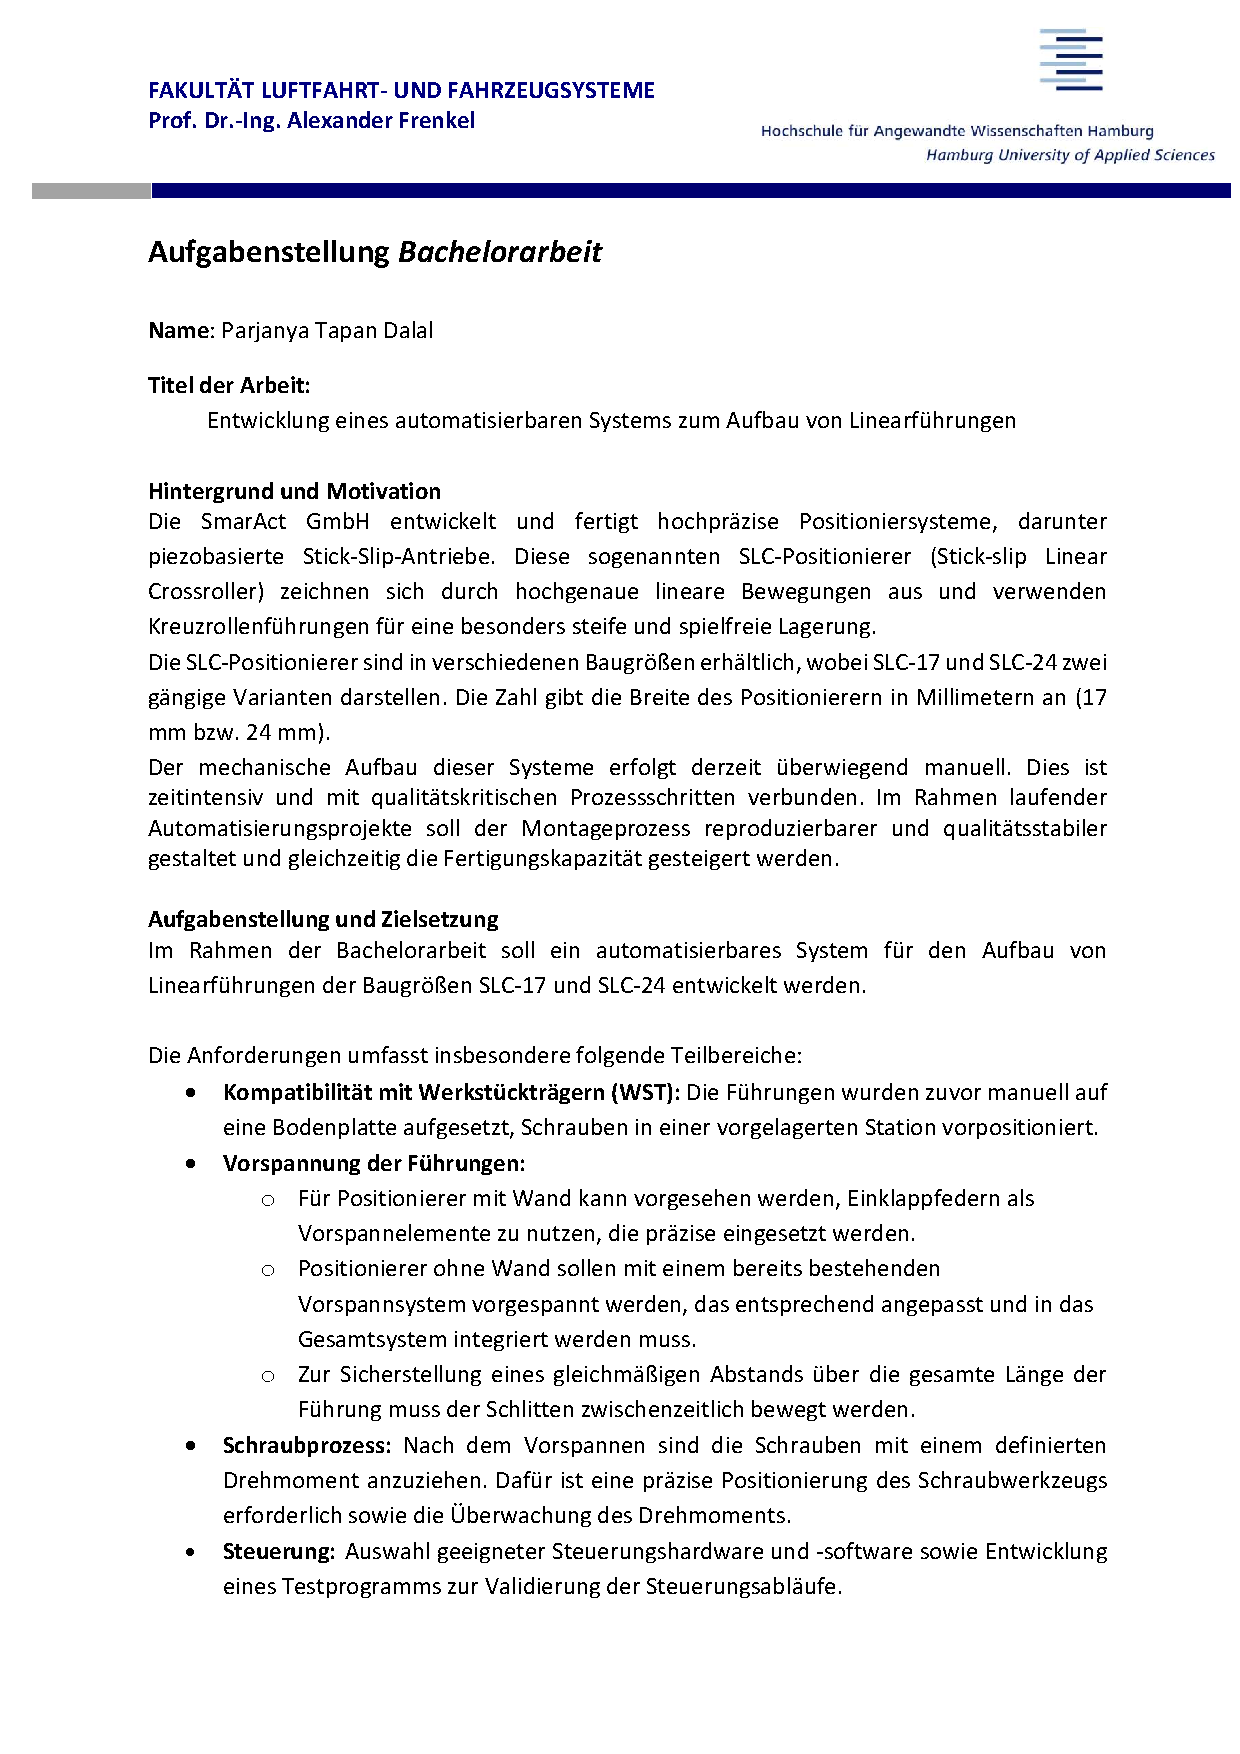
\includepdf[pages={-}]{misc/Background/aufgabenstellung.pdf}

\clearpage

% =========================================================
% Frontmatter-Nummerierung (römisch)
% =========================================================
\pagenumbering{Roman}
\setcounter{page}{1}

% =========================================================
% AB HIER: Kopfzeile AKTIV (ab Inhaltsverzeichnis)
% =========================================================
\pagestyle{fancy}

% Sicherheit: genügend Platz für Header
\setlength{\headheight}{18pt}

% Sicherheit: Kopfzeilenlinie erzwingen (falls irgendwo auf 0 gesetzt)
\renewcommand{\headrulewidth}{0.4pt}
\renewcommand{\footrulewidth}{0pt}

% Inhaltsverzeichnis
\maintoc
\clearpage

% Abbildungs- und Tabellenverzeichnis
\listoffigures
\clearpage
\listoftables
\clearpage

% Abkürzungsverzeichnis
\printglossary[type=acronym,style=acrotab, title = Abkürzungen]
% Symbolverzeichnis
\printglossary[type=symbols, style=symboltablr, title = Nomenklatur]
\clearpage

% =========================================================
% Ab hier: Hauptteil (arabisch)
% =========================================================
\setcounter{table}{0}
\renewcommand{\arraystretch}{1.15}
\pagenumbering{arabic}

%\pagestyle{fancy}
%\fancyhf{}
%\fancyhead[L]{HEADER-TEST-LEFT}
%\fancyhead[R]{\thepage}
%\renewcommand{\headrulewidth}{0.4pt}

%% Kapitel ab hier
\section{Einleitung}
\subsection{Motivation und Hintergrund}
Die Automatisierung in der Produktion spielt in der Industrie eine wichtige Rolle, besonders im Bereich der Präzisionstechnik, wo die Anforderungen an Prozesssicherheit, Reproduzierbarkeit und gleichbleibende Produktqualität steigen. Dagegen führen die manuellen Montageprozesse zu einer Abhängigkeit von der Erfahrung des jeweiligen Bedienpersonals und sind nur eingeschränkt skalierbar. Zusätzlich werden hierfür Fachkräfte mit sehr spezifischen Fähigkeiten benötigt, deren Verfügbarkeit bei steigenden Produktionsmengen nicht immer gegeben ist, wodurch sich die Skalierbarkeit weiter einschränkt.\cite{Groover_Automation, Lotter_Montage}

Die SmarAct GmbH entwickelt und fertigt hochpräzise Positioniersysteme für Anwendungen in den Lebenswissenschaften und der Lichtmikroskopie, in Hochenergie-Forschungs\-einrichtungen sowie in der Materialwissenschaft und Mikroskopie und in der Halbleiter- und Photonikindustrie.\cite{SmarAct_Company} Ein Produkt, das in hohen Stückzahlen hergestellt wird, ist der Positionierer vom Typ SLC (Stick-Slip Linear with Crossroller). Diese Systeme zeichnen sich durch eine Positioniergenauigkeit im Nanometerbereich, eine kompakte Bauweise sowie spielfreie Lager aus, die durch den Einsatz von Kreuzrollenführungen realisiert werden.\cite{SmarAct_SLC}

Die mechanische Montage von Linearführungen erfolgt derzeit überwiegend manuell. Mit steigenden Produktionsmengen und Qualitätsanforderungen besteht jedoch die Notwendigkeit, diesen Montageprozess reproduzierbarer zu gestalten und langfristig zu automatisieren. Ziel ist es, die Prozessstabilität zu erhöhen und gleichzeitig die Produktionskapazität zu steigern.

\subsection{Problemstellung}
Die Montage von Linearführungen ist ein qualitätskritischer Prozessschritt bei der Produktion von hochpräzisen Positioniersystemen.\cite{Lotter_Montage} Insbesondere haben die seitliche Vorspannung des Führungspakets und das Anziehen des Schraubendrehers mit einem vorgegebenen Drehmoment einen wesentlichen Einfluss auf die Steifigkeit und Lebensdauer der Linearachsen.\cite{VDI2230, Roloff_Matek}

Die seitliche Vorspannung bezeichnet das gezielte Einbringen einer Querlast in das Führungssystem, um einen spielfreien Kontakt zwischen Führungspaket und den Schlitten herzustellen und dadurch Nick- und Gier-Abweichungen der Linearachse zu reduzieren.

Beim derzeitigen manuellen Montageprozess können Abweichungen bei der Ausrichtung zwischen den Führungsteilen und beim auf die Schrauben ausgeübten Drehmoment auftreten. Diese Abweichungen führen zu einer reduzierten Reproduzierbarkeit der Montageergebnisse, wie Ablaufsgenauigkeit und laterale Steifigkeit, und erhöhen den Aufwand für Tests und Nacharbeiten. Darüber hinaus ist eine kontinuierliche Überwachung und Dokumentation der Prozessparameter im manuellen Betrieb nur eingeschränkt möglich.\cite{Groover_Automation}

Eine zusätzliche Herausforderung ergibt sich aus den unterschiedlichen Ausführungsvarianten der SLC-Positionierer. Je nach Bauform erfolgt die Vorspannung der Linearführungen entweder über integrierte mechanische Elemente oder über ein extern genutztes Vorspannsystem. Diese Variantenvielfalt muss bei der Entwicklung eines einheitlichen automatisierten Montageprozesses berücksichtigt werden und stellt besondere Anforderungen an die Flexibilität des zu entwickelnden Systems.

\subsection{Wissenschaftliche und technische Relevanz}
Aus wissenschaftlicher Sicht lässt sich diese Arbeit dem Bereich der Montage- und Automatisierungstechnik zuordnen. Die automatisierte Erzeugung definierter Vorspannkräfte und die kontrollierte Befestigung von Schrauben unter Berücksichtigung von Drehmoment- und Kraftwerten gehören zu den zentralen Themen der Präzisionsmontage.\cite{Lotter_Montage,Groover_Automation}

Aus technischer Sicht leistet diese Arbeit einen Beitrag zur Entwicklung eines modularen und anpassungsfähigen Montagesystems, das verschiedene Produktvarianten innerhalb eines standardisierten Prozesses verarbeiten kann. Durch den Einsatz motorisierter Bewegungssysteme, geeigneter Sensorik und einer strukturierten Steuerungsarchitektur lassen sich Montageprozesse nicht nur automatisieren, sondern auch validieren und dokumentieren.\cite{Kagermann_I40}

Die Ergebnisse sind sowohl für die industrielle Praxis als auch für die weitere Entwicklungsarbeit relevant, da sie die Grundlage für den späteren Transfer in einen Serienfertigungsprozess bilden.

\subsection{Zielsetzung der Arbeit}

Das Ziel dieser Bachelorarbeit ist die Entwicklung eines automatisierbaren Systems zur Montage von SLC-17- und SLC-24-Linearführungen mit und ohne Wände. Das Ziel ist die Entwicklung eines Montagekonzepts, das eine präzise Vorspannung der Führungen und einen kontrollierten Schraubvorgang mit definiertem Drehmoment ermöglicht.

Im Rahmen der Arbeit werden zunächst die bestehenden Montageprozesse analysiert und daraus die Anforderungen abgeleitet. Auf dieser Grundlage werden geeignete Konzepte entwickelt, bewertet und konstruiert. Darüber hinaus werden geeignete Steuerungshardware und -software ausgewählt, wodurch die grundlegenden Systemfunktionen validiert werden.

\subsection{Vorgehensweise und Aufbau der Arbeit}
Die Bachelorarbeit ist in mehrere Kapitel unterteilt, die aufeinander aufbauen und den systematischen Entwicklungsprozess des Systems beschreiben.

Kapitel 2 beginnt mit einer Beschreibung von Industrie 4.0 und einer Analyse des bestehenden Montageprozesses für Linearführungen. Insbesondere werden die Prozessschritte identifiziert, die automatisiert werden sollen. Kapitel 3 beschreibt die methodische Vorgehensweise der Arbeit. Hier wird die VDI-Richtlinie 2221 \enquote{Entwicklung technischer Produkte und Systeme} als theoretische Grundlage für den weiteren Entwicklungsprozess vorgestellt.

Kapitel 4 befasst sich mit der Entwicklung und Bewertung verschiedener Konzepte zur Umsetzung der Vorspannung, des Einschraubvorgangs und der erforderlichen Bewegungen. Das ausgewählte Konzept wird dann in Kapitel 5 umgesetzt. Kapitel 6 befasst sich mit der Validierung des entwickelten Systems und der Auswertung der Ergebnisse.

In Kapitel 7 werden die Ergebnisse diskutiert, eine Schlussfolgerung abgeleitet und ein Ausblick auf mögliche Weiterentwicklungen gegeben. Abschließend fasst Kapitel 8 diese Arbeit zusammen.
\clearpage
\section{Stand der Technik}

\subsection{Grundlagen der Automatisierung in der Fertigung}
Die Automatisierung von Fertigungs- und Montageprozessen ist sehr wichtig für moderne Produktionssysteme. Ziel ist es, manuelle Tätigkeiten zu reduzieren, Prozessschritte zu standardisieren und eine gleichbleibende Produktqualität sicherzustellen sowie die Produktionskapazität zu erhöhen, indem mit derselben Personalstärke eine größere Anzahl von Einheiten hergestellt werden kann. Abhängig vom Automatisierungsgrad kommen dabei teilautomatisierte oder vollständig automatisierte Systeme zum Einsatz.

In der Montage werden automatisierte Systeme besonders dort eingesetzt, wo hohe Anforderungen an Wiederholgenauigkeit, Prozesssicherheit und Dokumentation bestehen. Automatisierung wird auch dort eingesetzt, wo der Mensch entlastet werden soll oder menschliche Arbeitskraft eingespart beziehungsweise gezielter für höherwertige, komplexe oder überwachende Tätigkeiten eingesetzt werden kann. Dies betrifft sowohl anspruchsvolle Montageaufgaben als auch stark repetitive und monotone Arbeitsprozesse.

Typische Anwendungsfelder sind das Positionieren von Bauteilen, das kontrollierte Einbringen von Kräften sowie das Verschrauben mit definierten Parametern. Neben der reinen Ausführung der Montageaufgaben spielt auch die Überwachung des Prozesses eine wichtige Rolle, um Abweichungen frühzeitig erkennen zu können.\cite{Groover_Automation,Lotter_Montage}

\subsection{Industrie 4.0 im Kontext der Montage}
Im Montageumfeld steht Industrie 4.0 vor allem für den Wandel von starren, fest definierten Abläufen hin zu flexiblen und vernetzten Montagesystemen. Maschinen, Werkzeuge und IT-Systeme sind miteinander verbunden und tauschen kontinuierlich Informationen aus. Dadurch lassen sich Montageschritte besser aufeinander abstimmen und Produktionsprozesse können schneller an neue Produkte, Varianten oder Stückzahlen angepasst werden. Diese Flexibilität gewinnt nicht nur bei kundenindividuellen Produkten, sondern auch bei hohen Stückzahlen zunehmend an Bedeutung.\cite{Kagermann_I40}

Ein weiterer zentraler Punkt ist der Umgang mit Daten. Während der Montage werden zahlreiche Prozessdaten erfasst, etwa zu Kräften, Zeiten oder Qualitätsmerkmalen. Diese Daten machen den Montageprozess transparenter und ermöglichen es, Schwachstellen zu erkennen und Abläufe schrittweise zu verbessern. Gleichzeitig verändert sich die Rolle des Menschen in der Montage: Digitale Assistenzsysteme können unterstützen, indem sie Informationen bereitstellen oder bei komplexen Arbeitsschritten helfen. Der Mensch bleibt dabei ein entscheidender Faktor, wird jedoch durch vernetzte und intelligente Systeme sinnvoll ergänzt.

Erste Elemente einer vernetzten Produktionsumgebung sind im Unternehmen bereits umgesetzt. Bei der SmarAct GmbH besteht eine Anbindung der Montage- und Prüfsysteme an das zentrale ERP-System. Die einzelnen Systeme greifen dabei auf im ERP hinterlegte Informationen zurück, beispielsweise auf Prüfparameter oder auftragsbezogene Vorgaben.

Durch diese Anbindung wird sichergestellt, dass die für einen Auftrag relevanten Parameter einheitlich und in aktueller Version an den jeweiligen System zur Verfügung stehen. Gleichzeitig entsteht eine durchgängige Verbindung zwischen Montage- und Prüfschritten, bei der Informationen systemseitig weitergegeben werden. Diese vorhandene Infrastruktur bildet eine sinnvolle Grundlage für eine weitergehende Automatisierung und Digitalisierung von Montageprozessen.

\subsection{Unternehmensprofil und Produktumfeld}
Die SmarAct GmbH entwickelt und fertigt hochpräzise Positioniersysteme mit Genauigkeiten im Nanometerbereich. Die Produkte kommen unter anderem in der Halbleitertechnik, Optik, Medizintechnik sowie in der Forschung zum Einsatz. Charakteristisch für diese Anwendungen sind hohe Anforderungen an Genauigkeit, Wiederholbarkeit und Langzeitstabilität.\cite{SmarAct_Company}

Ein wesentlicher Bestandteil des Produktportfolios sind die piezobasierten SMARSLIDE-Linearpionierer der Serie SLC, die auf dem Stick-Slip-Prinzip basieren. Diese Antriebstechnologie ermöglicht eine sehr hohe Positionierauflösung bei gleichzeitig kompakter Bauweise. Aufgrund der geringen Baugrößen und der engen Toleranzen stellen sowohl die Fertigung als auch die Montage dieser Systeme besondere Anforderungen an Präzision und Prozesssicherheit.

Die SLC-Serie ist in unterschiedlichen Bauformen erhältlich, die sich im Wesentlichen durch ihre Breite und Länge unterscheiden. Die SLC-17-Positionierer besitzen eine Breite von 17 mm und sind für Anwendungen mit besonders begrenztem Bauraum ausgelegt. Die SLC-24-Positionierer weisen eine Breite von 24 mm auf und bieten aufgrund ihrer größeren Bauform eine erhöhte mechanische Steifigkeit.

Zusätzlich unterscheiden sich die Positionierer hinsichtlich ihrer konstruktiven Ausführung. Die Standardausführung der SLC-Positionierer verfügt über eine sockel-förmige Bodenplatte. Ergänzend dazu wurden Varianten mit Wand entwickelt, um die mechanische Belastbarkeit zu erhöhen. Diese Ausführungen besitzen eine U-förmige Bodenplatte und wird als SLC-W bezeichnet.\cite{SmarAct_SLC}

Diese konstruktiven Unterschiede beeinflussen insbesondere den Aufbau der Linearführung sowie das erforderliche Vorspannkonzept. Darüber hinaus sind spezielle Ausführungen für den Einsatz im Hoch- und Ultrahochvakuum sowie unterschiedliche Materialkombinationen verfügbar.

\begin{figure}[htbp]
    \centering
    \begin{subfigure}[t]{0.48\linewidth}
        \centering
        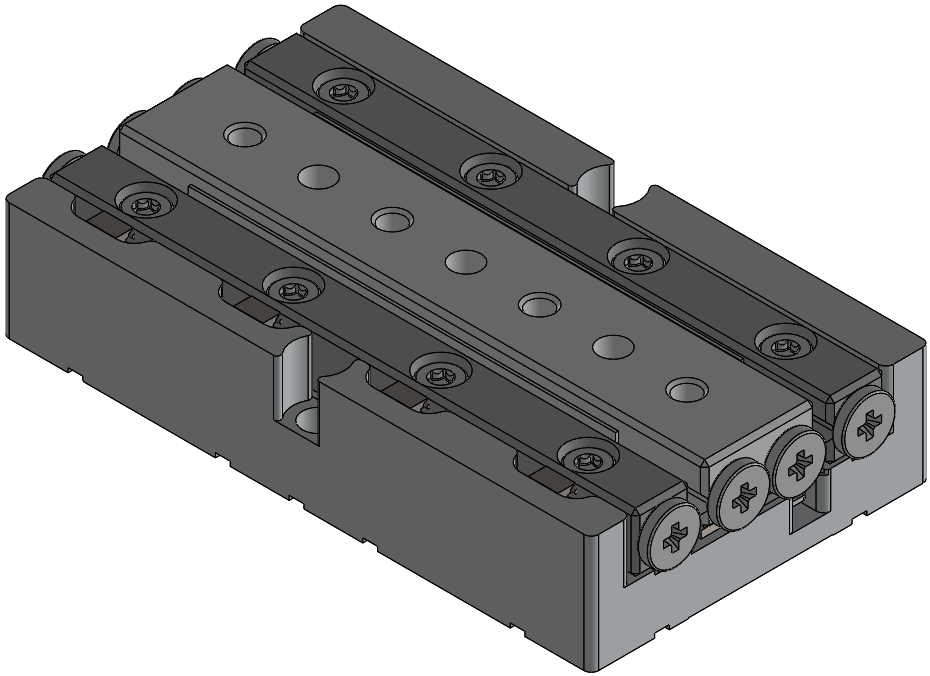
\includegraphics[width=\linewidth]{Bilder/02_Stand_der_Technik/SLC-1740-W.png}
        \caption{SLC-1740-W}
        \label{fig:slc1740_mit_wand}
    \end{subfigure}
    \hfill
    \begin{subfigure}[t]{0.48\linewidth}
        \centering
        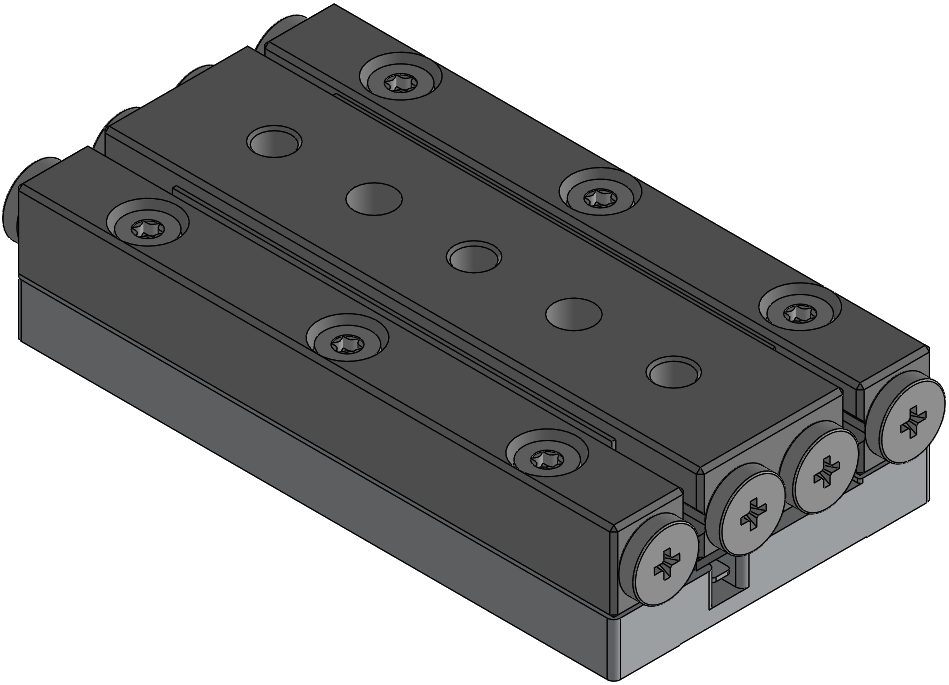
\includegraphics[width=\linewidth]{Bilder/02_Stand_der_Technik/SLC-2445.png}
        \caption{SLC-2445}
        \label{fig:slc2445}
    \end{subfigure}
    \caption{Bauformen der SLC-Positionierer mit unterschiedlichen Breiten und Bodenplattenausführungen (interne CAD-Daten)}
    \label{fig:slc_bauformen}
\end{figure}

\subsection{Aufbauprozess der SLC-Positionierer}
Der Aufbau der SLC-Positionierer erfolgt in mehreren aufeinander abgestimmten Montageschritten, bei denen insbesondere die Ausrichtung der Linearführung und die Einstellung der Vorspannung eine zentrale Rolle spielt.

Zu Beginn wird die Bodenplatte des Positionierers auf dem vorgesehenen Werkstückträger (auch Interface genannt) positioniert und fest verschraubt. Anschließend dient der Werkstückträger als Referenz- und Aufnahmeeinheit für die nachfolgenden Montageschritte, bei denen der vormontierte Piezoantrieb sowie die Positionssensorik (Encoder) mithilfe geeigneter Einbauhilfen in der Bodenplatte platziert und befestigt werden.

Diese Komponenten bilden die funktionale Basis des Positionierers und müssen bereits in dieser frühen Phase korrekt ausgerichtet sein, da spätere Korrekturen nur mit erheblichem Aufwand möglich sind.

Im nächsten Schritt wird der Schlitten gemeinsam mit den Kreuzrollen und dem Führungspaket auf die Bodenplatte aufgelegt. Eine Seite des Führungspakets wird dabei gezielt gegen eine vertikale, gerade Referenzfläche ausgerichtet. Dadurch wird sichergestellt, dass diese Seite des Führungspakets parallel zur Bodenplatte liegt. Anschließend wird die ausgerichtete Seite mit der Bodenplatte verschraubt.

\begin{figure}[htbp]
    \centering
    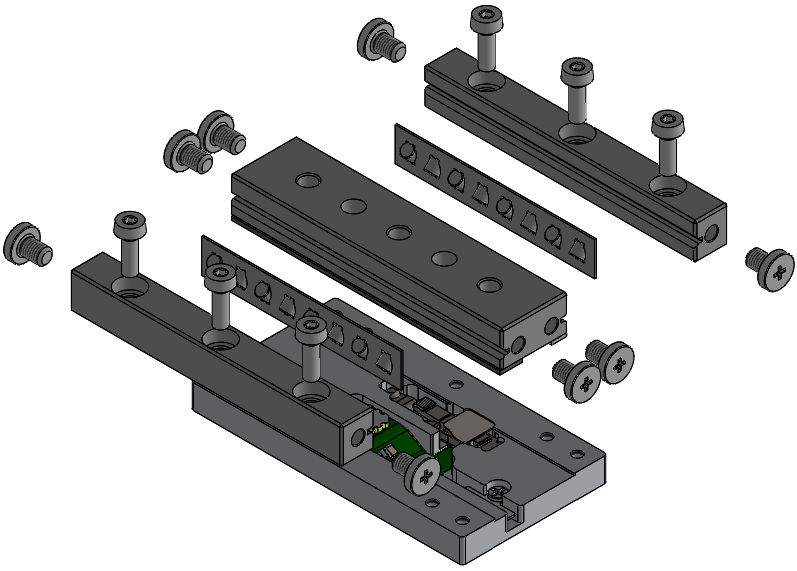
\includegraphics[width=0.5\linewidth]{Bilder/02_Stand_der_Technik/slc-explosion.png}
    \caption{Explosionsansicht der SLC-2445 Positionierer (basierend auf interne CAD-Daten)}
    \label{fig:slc2445_explosion}
\end{figure}

Nach diesem Montageschritt wird das Führungspaket vorgespannt, sodass das vorhandene Spiel zwischen Schlitten, Kreuzrollen und Führungselementen reduziert beziehungsweise vollständig eliminiert wird. Nach dem Einbringen der Vorspannung wird die gegenüberliegende Seite des Führungspakets verschraubt, wodurch die Position der Linearführung fixiert wird.

\subsection{Besonderheiten beim Aufbau von SLC-W-Positionierern}
Der grundlegende Aufbauprozess der SLC-W-Positionierer entspricht dem der Standard-SLC-Varianten. Der wesentliche Unterschied liegt in der Art und Weise, wie die Vorspannung eingebracht wird. Bei den Positionierern mit Wand erfolgt die Vorspannung nicht direkt über die Bodenplatte, sondern mithilfe von Keilen, die zwischen der Wand und einer Seite des Führungspakets positioniert werden.

Durch das gezielte Eindrücken dieser Keile wird eine definierte Vorspannkraft auf das Führungspaket aufgebracht. Die dabei von oben eingeleitete Kraft wird durch die Keilgeometrie in eine laterale Kraft auf das Führungspaket umgesetzt.

Beim anschließenden Verschrauben der gegenüberliegenden Seite ist es erforderlich, den Schlitten kontrolliert mitzubewegen. Dies ist erforderlich, da die angeordneten Rollenkäfige kürzer sind als die Gesamtlänge der Führung. Ohne ein Mitführen des Schlittens würde sich der wirksame Abstand zwischen den beiden Seiten des Führungspakets entlang der Führungsachse verändern.

Durch das gezielte Mitbewegen des Schlittens wird sichergestellt, dass der Abstand zwischen den beiden Seiten des Führungspakets über die gesamte Länge konstant bleibt und die Linearführung parallel ausgerichtet ist. Dadurch werden Verspannungen sowie geometrische Abweichungen innerhalb der Führung vermieden.

\begin{figure}[htbp]
    \centering
    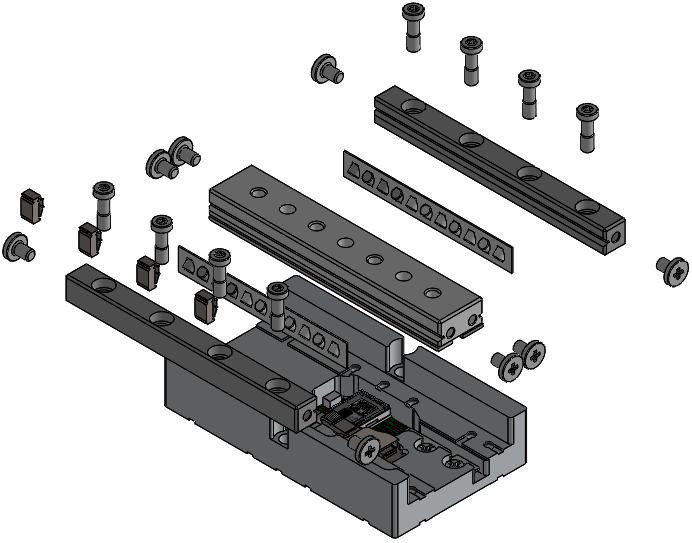
\includegraphics[width=0.5\linewidth]{Bilder/02_Stand_der_Technik/slc-w-explosion.png}
    \caption{Explosionsansicht der SLC-1740-W Positionierer (basierend auf interne CAD-Daten)}
    \label{fig:slc1740w_explosion}
\end{figure}

\subsection{Bedeutung der Vorspannung für die Funktion des Positionierers}
Die Vorspannung der Linearführung ist von entscheidender Bedeutung für die Funktion und Leistungsfähigkeit der SLC-Positionierer. Sie dient dazu, Roll-, Nick- und Gierbewegungen des Schlittens während der Bewegung durch den Piezoantrieb zu minimieren. Ohne eine korrekt eingestellte Vorspannung kann es zu Spiel innerhalb der Führung kommen, was sich unmittelbar negativ auf das Bewegungsverhalten auswirkt.\cite{Roloff_Matek}

Eine unzureichende Vorspannung kann zu verminderter Positioniergenauigkeit sowie reduzierter Steifigkeit führen. Darüber hinaus verschlechtert sich die Winkelgenauigkeit, insbesondere in Bezug auf Nick- und Gierbewegungen des Schlittens. Dies ist insbesondere bei Mikro- und Nanopositionieranwendungen kritisch, da selbst kleinste Abweichungen zu messbaren Positionsfehlern führen können.\cite{VDI2230}

Eine definierte und reproduzierbare Vorspannung ist daher eine grundlegende Voraussetzung für eine hohe Genauigkeit, stabile Bewegungsabläufe und eine zuverlässige Funktion der Positionierer. Aus diesem Grund stellt die Einstellung der Vorspannung einen besonders qualitätskritischen Montageschritt dar und ist von zentraler Bedeutung für eine mögliche Automatisierung des Aufbauprozesses.

Die Auswirkungen der Führungsgeometrie und der eingestellten Vorspannung lassen sich unter anderem anhand der Winkelabweichungen des Schlittens beschreiben.

\begin{figure}[htbp]
    \centering
    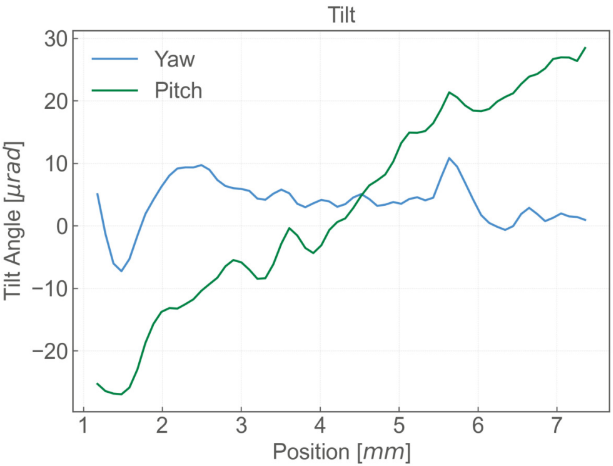
\includegraphics[width=0.5\linewidth]{Bilder/02_Stand_der_Technik/Vorspannung_Pitch_Yaw.png}
    \caption{Pitch- und Yaw-Abweichungen des Schlittens in Abhängigkeit vom Verfahrweg (basierend auf internen Produktdaten)}
    \label{fig:pitch_yaw_graph}
\end{figure}

Die in Abbildung~\ref{fig:pitch_yaw_graph} dargestellten Verläufe von Nicken (Pitch) und Gieren (Yaw) über den Verfahrweg zeigen, dass selbst geringe geometrische Abweichungen innerhalb der Linearführung messbare Winkeländerungen verursachen. Eine ungleichmäßige oder unzureichende Vorspannung kann diese Effekte verstärken und sich negativ auf die Positioniergenauigkeit auswirken.

\subsubsection{Ermittlung und Variation der Vorspannkräfte}
Zur Ermittlung der Vorspannkräfte wurden als Ausgangspunkt die vom Hersteller empfohlenen Einstellungen zur Vorspannung verwendet, die im Rahmen der Produktdokumentation intern zur Verfügung gestellt wurden. Diese basieren auf den angegebenen Einstellmomenten der Justierschrauben bzw. den dazugehörigen empfohlenen Vorspann-Einstellungen. Daraus wurde eine Referenz-Vorspannkraft $F_A$ (Herstellerwert) abgeleitet und als Vergleichsbasis festgelegt. Für die Versuche wurden die Kräfte anschließend gezielt variiert, um den Einfluss einer zu niedrigen bzw. zu hohen Vorspannung systematisch bewerten zu können.

Es wurde jeweils eine manuelle Vorspannung nach Arbeitsanweisung eingestellt, um eine praxisnahe Referenz zu erhalten. Danach wurden definierte Kraftstufen auf Basis von $F_A$ eingestellt ($F_A$, $1{,}5\cdot F_A$, $2\cdot F_A$, $2{,}5\cdot F_A$).

Für jede Stufe wurde derselbe Messablauf durchgeführt:
\begin{enumerate}
    \item Vorspannen
    \item Rollwiederstandsmessung
    \item Krafteinstellung
    \item Aktorvermessung
\end{enumerate}

Als Qualitätskennwerte wurden unter anderem Rollreibung, Krümmung (vertikal/horizontal), Umkehrfehler sowie Wiederholgenauigkeiten ausgewertet.

Die Ergebnisse zeigen, dass eine Erhöhung der Vorspannung zunächst zu einer deutlichen Reduktion von Spiel- und Umkehreffekten führt und damit insbesondere Umkehrfehler sowie die Wiederholgenauigkeit verbessert. Bei zu hoher Vorspannung nehmen jedoch einzelne Kennwerte wieder zu (z.\,B. durch steigende Reibung bzw. zusätzliche elastische Verformungen). Über beide Baugrößen hinweg lieferte eine Vorspannung von ungefähr $2\cdot F_A$ den besten Kompromiss aus geringer Rollreibung, stabiler Führungsgeometrie und guter Wiederholgenauigkeit. Diese Kraftstufe wurde daher als bevorzugter Zielwert für die weitere Auslegung des (automatisierten) Vorspannprozesses abgeleitet.

\subsection{Bestehende Montageprozesse im Unternehmen}
Der Aufbau der Linearführungen innerhalb der Positioniersysteme erfolgt derzeit überwiegend manuell. Die Montage umfasst das Aufsetzen der Führungen, das Einbringen der Vorspannelemente sowie das anschließende Verschrauben der Komponenten. Diese Arbeitsschritte erfordern ein hohes Maß an Sorgfalt und Erfahrung, da sie direkten Einfluss auf die Funktionalität des Endprodukts haben.

Die Einstellung der Vorspannung wird abhängig von der jeweiligen Bauform unterschiedlich realisiert. Für die Standardausführungen der SLC-Positionierer existiert bereits eine separate Vorspannvorrichtung, an der das Führungspaket manuell positioniert und vorgespannt wird. Die Vorrichtung besteht im Wesentlichen aus einem seitlich wirkenden Schieber, der das Führungspaket mit einer definierten Kraft zusammendrückt. Bei Positionierern mit Wand (SLC-W) wird die Vorspannung zusätzlich durch das Einbringen von Keilen erzeugt. Hierzu kommt ein Stößel zum Einsatz, der den jeweiligen Keil vertikal bis zu einer definierten Distanz in das System einpresst.

Abgesehen von diesen beiden Systemen erfolgt der überwiegende Teil des Montageprozesses händisch. Insbesondere das Ausrichten der Bauteile, das kontrollierte Verschrauben sowie die Überprüfung der Parallelität und Beweglichkeit des Schlittens liegen vollständig in der Verantwortung der ausführenden Person. Eine durchgängige Automatisierung oder Integration der einzelnen Montageschritte ist derzeit nicht gegeben.

\subsubsection{SLC-Vorspannsystem}
Das SLC-Vorspannsystem dient der gezielten Einstellung der seitlichen Vorspannung zwischen Führungspaket und Schlitten während des Montageprozesses. Es kommt als eigenständiges Vorspannsystem zum Einsatz und wird vor dem eigentlichen Schraubprozess verwendet.

Die Vorspannung wird über einen linear geführten Schieber realisiert, der das Führungspaket kontrolliert in Richtung des Schlittens verschiebt. Der Schieber ist mechanisch geführt und wird über eine Spindel mit Nut angetrieben, wodurch eine rein translatorische Bewegung mit definiertem Kraftangriff ermöglicht wird. Der maximale Verfahrweg des Vorspannsystems beträgt 49,5 mm und deckt damit alle erforderlichen Baugrößen innerhalb der SLC-Produktfamilie ab.

Während des Vorspannvorgangs wird das Führungspaket gegen den Schlitten gedrückt und in dieser Position gehalten. In diesem Zustand erfolgt der nachfolgende Schraubprozess, sodass die eingestellte Vorspannung während der Verschraubung konstant erhalten bleibt. Auf diese Weise wird sichergestellt, dass sich die Kontaktverhältnisse innerhalb der Linearführung nicht unkontrolliert verändern.

Der Kraftfluss innerhalb des Vorspannsystems erfolgt ausschließlich über starre mechanische Bauteile. Der Einsatz elastischer Elemente wird bewusst vermieden, um eine hohe Reproduzierbarkeit der eingestellten Vorspannung zu gewährleisten. Zur Erfassung und Überwachung der aufgebrachten Vorspannkraft ist eine Kraftmessdose direkt in den Kraftfluss integriert. Dadurch kann die eingeleitete Kraft messtechnisch erfasst und überprüft werden.

Zur Absicherung des Bewegungsbereichs sind zwei Gabellichtschranken als Endlagensensoren vorgesehen. Diese begrenzen den maximal zulässigen Verfahrweg des Schiebers und schützen das System vor mechanischer Überlastung.

Abbildung~\ref{fig:SLC_Vorspannsystem} zeigt das Vorspannsystem als eigenständige mechanische Baugruppe.

\begin{figure}[htbp]
    \centering
    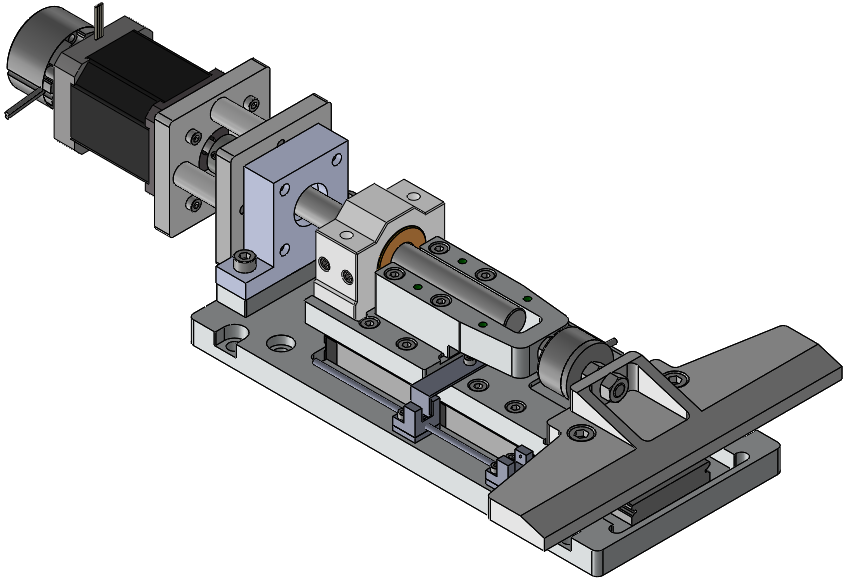
\includegraphics[width=0.5\linewidth]{Bilder/02_Stand_der_Technik/SLC_Vorspannen.png}
    \caption{Darstellung des SLC-Vorspannsystems}
    \label{fig:SLC_Vorspannsystem}
\end{figure}

\subsubsection{Keile-Einpresssystem}
Für Positionierer der Bauform SLC-W wird die Vorspannung zusätzlich über Keile eingestellt. Hierfür kommt ein separates Keileinpresssystem zum Einsatz, das den seitlichen Vorspannprozess ergänzt. Ziel dieses Systems ist es, die Keile kontrolliert und reproduzierbar in das Führungssystem einzubringen.

Der grundsätzliche Aufbau des Keileinpresssystems ist dem zuvor beschriebenen Vorspannsystem ähnlich, unterscheidet sich jedoch in der Bewegungsrichtung und der Art der Krafteinleitung. Während das Vorspannsystem eine seitlich wirkende Kraft auf das Führungspaket ausübt, erfolgt der Einpressvorgang beim Keilsystem vertikal. Der Keil wird dabei von oben in die vorgesehene Aufnahme eingepresst.

Die Bewegung des Einpressstempels erfolgt über einen linearen Aktor, der eine präzise Zustellung in Z-Richtung ermöglicht. Durch die lineare Führung wird sichergestellt, dass der Keil ohne Verkanten eingebracht wird und die Kraft senkrecht zur Führungsgeometrie wirkt. Der Einpressvorgang erfolgt ausschließlich translatorisch.

Zur Überwachung der aufgebrachten Einpresskraft ist eine Kraftmessdose direkt in den Kraftfluss integriert. Dadurch kann der Einpressvorgang kontrolliert überwacht und reproduzierbar durchgeführt werden.

Zur Absicherung des Bewegungsbereichs sind zwei Gabellichtschranken als Endlagensensoren vorgesehen. Diese erfassen die obere und untere Endlage des Einpressstempels und begrenzen den zulässigen Verfahrweg des Aktors. Dadurch wird ein sicherer Betrieb gewährleistet und gleichzeitig eine reproduzierbare Referenzierung des Systems ermöglicht.

\begin{figure}[H]
    \centering
    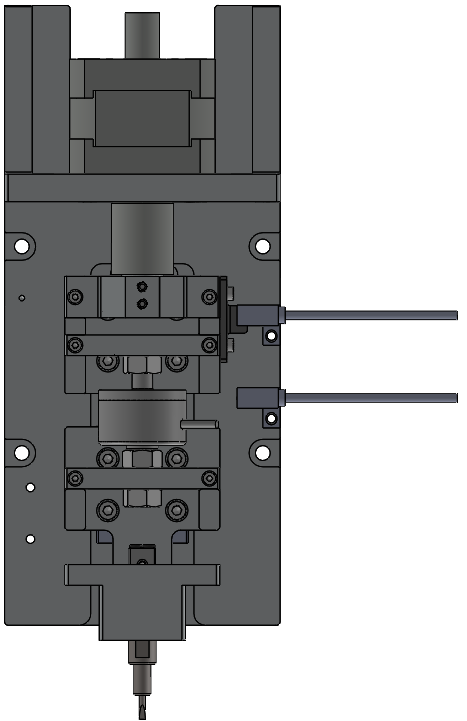
\includegraphics[width=0.5\linewidth]{Bilder/02_Stand_der_Technik/Keile_Einpress.png}
    \caption{Keile-Einpress System}
    \label{fig:keile_einpress}
\end{figure}

\subsection{Stand der Automatisierung im Unternehmen}
Der Automatisierungsgrad im Unternehmen unterscheidet sich deutlich zwischen Montage- und Testprozessen. Während der Aufbau der Positioniersysteme derzeit überwiegend manuell erfolgt, sind die nachgelagerten Prüfprozesse bereits in hohem Maße automatisiert.

Im Bereich der Montage existieren bislang lediglich einzelne, teilautomatisierte Hilfsmittel. Dazu zählen eine Vorspannvorrichtung für die Standardausführungen der SLC-Position\-ierer sowie eine separate Keileinpresssystem für Positionierer mit integrierter Wand (SLC-W). Diese Vorrichtungen unterstützen jeweils einzelne Prozessschritte, sind jedoch nicht miteinander verknüpft und nicht in einen durchgängigen Montageablauf integriert. Der Großteil der qualitätskritischen Tätigkeiten, wie das Ausrichten der Linearführung, das kontrollierte Einbringen der Vorspannung sowie das Verschrauben der Komponenten, wird weiterhin manuell durchgeführt. Die Qualität des Montageergebnisses hängt dabei in hohem Maße von der Erfahrung und Sorgfalt der ausführenden Person ab.

Demgegenüber ist der nachgelagerte Testprozess bereits weitgehend automatisiert und erlaubt eine reproduzierbare sowie strukturierte Erfassung der Funktions- und Qualitätsmerkmale der Positionierer. Der hohe Automatisierungsgrad im Testbereich verdeutlicht, dass insbesondere der Montageprozess aktuell den verbleibenden manuellen und qualitätskritischen Abschnitt innerhalb der Prozesskette darstellt und damit ein zentrales Potenzial für eine weitere Automatisierung bietet.

\subsection{Einordnung der Arbeit in den Stand der Technik}
Die vorliegende Arbeit ist im Spannungsfeld zwischen hochautomatisierten Testprozessen und weitgehend manuellen Montageabläufen einzuordnen. Während im Unternehmen bereits umfangreiche Erfahrungen mit der Automatisierung komplexer Prüfprozesse bestehen, sind qualitätskritische Montageschritte bislang nur begrenzt standardisiert und reproduzierbar.

Ziel dieser Arbeit ist es, den Montageprozess der Linearführungen von SLC-Positionierern in seinen qualitätskritischen Teilschritten zu verstehen und daraus ein automatisierbares Montagekonzept abzuleiten. Im Vordergrund stehen dabei die reproduzierbare Einstellung der seitlichen Vorspannung sowie das nachfolgende Fixieren der seitlichen Führungselemente. Ergänzend werden die notwendigen Prozessschnittstellen beschrieben, die eine strukturierte Bauteilführung, ein definiertes Referenzieren und eine sichere Handhabung während der Montage ermöglichen.

Durch die Entwicklung eines modularen und erweiterbaren Montagekonzepts soll ein Beitrag zur schrittweisen Erhöhung des Automatisierungsgrads geleistet werden. Gleichzeitig ermöglicht das Konzept eine verbesserte Prozesskontrolle und Dokumentation qualitätsrelevanter Parameter (z. B. Vorspannkraft und Schraubparameter). Die Arbeit überträgt damit etablierte Prinzipien der Automatisierung der Fertigung gezielt auf die spezifischen Anforderungen hochpräziser Positioniersysteme der SmarAct GmbH.
\clearpage
\section{Methodik}

Die methodische Vorgehensweise dieser Arbeit orientiert sich an der Richtlinie 
VDI~2221, welche ein systematisches Vorgehen zur Entwicklung technischer Systeme 
und Produkte beschreibt.\cite{VDI2221, MKon_VL}

Ziel der Richtlinie ist es, den Konstruktionsprozess 
strukturiert, nachvollziehbar und lösungsneutral zu gestalten sowie eine 
reproduzierbare Entscheidungsfindung zu ermöglichen.

Gemäß VDI~2221 erfolgt das Konstruieren nicht als strikt linearer Ablauf, sondern 
als iterativer Prozess. Zwischen den einzelnen Phasen sind Rückkopplungen vorgesehen, 
um neue Erkenntnisse aus späteren Entwicklungsschritten in frühere Phasen 
zurückführen zu können. Dieses iterative Vorgehen ist insbesondere bei komplexen 
technischen Systemen von Bedeutung und wurde auch in der vorliegenden Arbeit 
berücksichtigt.

Für die Entwicklung des automatisierbaren Systems wurden die folgenden 
methodischen Schritte angewendet:

\begin{itemize}
    \item \textbf{Klärung und Präzisierung der Aufgabenstellung}  

    Zu Beginn des Entwicklungsprozesses wurde die Aufgabenstellung analysiert und 
    präzisiert. Dabei wurden die Zielsetzung des Systems, die vorgesehenen Einsatzbedingungen 
    sowie relevante Randbedingungen und Einschränkungen erfasst. Zusätzlich wurde das 
    bestehende System betrachtet, um Schwachstellen, Verbesserungspotenziale und 
    funktionale Zusammenhänge zu identifizieren. Ziel dieser Phase ist gemäß VDI~2221 
    die eindeutige Beschreibung der Entwicklungsaufgabe als verbindliche Grundlage 
    für alle nachfolgenden Schritte.

    \item \textbf{Ermittlung der Anforderungen}  

    Aufbauend auf der geklärten Aufgabenstellung wurden die Anforderungen an das zu 
    entwickelnde System systematisch ermittelt und in einer Anforderungsliste 
    dokumentiert. Diese umfasst sowohl Muss- als auch Wunschanforderungen und 
    berücksichtigt funktionale, geometrische, wirtschaftliche sowie organisatorische 
    Aspekte. Die Anforderungsliste dient während des gesamten Entwicklungsprozesses 
    als zentrales Referenzdokument und bildet die Grundlage für die Bewertung und 
    Auswahl von Lösungsvarianten.

    \item \textbf{Funktionsanalyse}  

    In Anlehnung an die VDI~2221 wurde die Gesamtfunktion des Systems zunächst 
    lösungsneutral betrachtet und anschließend in Teilfunktionen zerlegt. Ziel der 
    Funktionsanalyse ist es, die funktionalen Zusammenhänge innerhalb des Systems 
    transparent darzustellen, ohne sich frühzeitig auf konkrete konstruktive 
    Lösungen festzulegen. Die Funktionsstruktur bildet damit die Basis für die 
    systematische Entwicklung alternativer Lösungsprinzipien.

    \item \textbf{Konzipieren}  

    Auf Grundlage der Funktionsstruktur wurden für die einzelnen Teilfunktionen 
    unterschiedliche Lösungsprinzipien entwickelt. Diese wurden zu mehreren 
    Gesamtkonzepten kombiniert. Zur Bewertung der entwickelten Konzepte wurde eine 
    Nutzwertanalyse durchgeführt. Ziel dieser Analyse war es, die Konzepte anhand 
    mehrerer, aus der Anforderungsliste abgeleiteter Bewertungskriterien systematisch 
    miteinander zu vergleichen und eine nachvollziehbare Entscheidungsgrundlage zu 
    schaffen.

    Die Bewertungskriterien wurden entsprechend ihrer Bedeutung für die 
    Aufgabenstellung gewichtet. Anschließend wurden die einzelnen Konzepte für jedes 
    Kriterium bewertet und die gewichteten Teilnutzen zu einem Gesamtnutzwert 
    zusammengefasst. Das für die weitere Entwicklung herangezogene Konzept wurde auf 
    Basis der Ergebnisse der Nutzwertanalyse ausgewählt.

    \item \textbf{Entwerfen und Ausarbeiten}  

    Das ausgewählte Konzept wurde im weiteren Verlauf schrittweise konstruktiv 
    ausgearbeitet. Dies umfasste unter anderem die Dimensionierung von Bauteilen, die 
    Auswahl geeigneter Norm- und Kaufteile sowie die Auslegung der Schnittstellen 
    zwischen den einzelnen Systemelementen. Entsprechend der VDI~2221 erfolgte dieser 
    Schritt iterativ, sodass Erkenntnisse aus Berechnungen, Simulationen oder 
    konstruktiven Überlegungen zu Anpassungen früherer Entscheidungen führen konnten.
\end{itemize}

Die VDI-2221-Methodik bildet somit den methodischen Rahmen für die Entwicklung des 
automatisierbaren Systems in dieser Arbeit. Durch die strukturierte Vorgehensweise 
wird eine nachvollziehbare und systematische Entwicklung sichergestellt, während 
gleichzeitig ausreichend Flexibilität für iterative Anpassungen erhalten bleibt.

\begin{figure}[htbp]
    \centering
    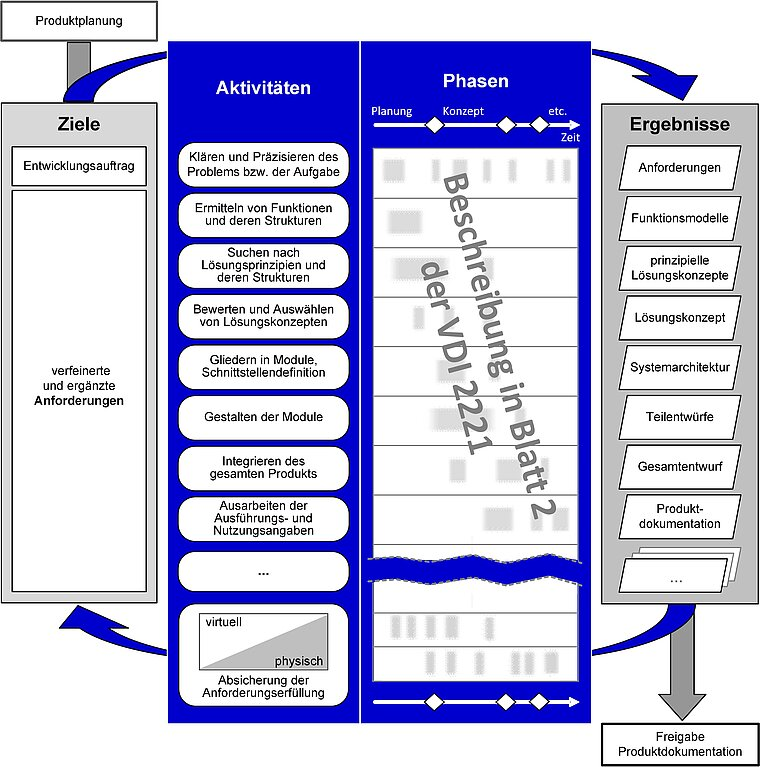
\includegraphics[width=0.8\linewidth]{Bilder/03_Methodik/VDI2221.jpg}
    \caption{Vorgehensmodell der Produktentwicklung nach VDI 2221 (Quelle: VDI 2221) \cite{VDI2221}}
    \label{fig:vdi}
\end{figure}
\clearpage
\section{Konzeptentwicklungsprozess}
\subsection{Klärung der Aufgabenstellung und Anforderungsanalyse}
\subsubsection{Ziel des Systems}
Ziel des Systems ist es, den Aufbau der Linearführungen für SLC-Positionierer der Baugrößen SLC-17 und SLC-24 so zu gestalten, dass eine spätere voll-Automatisierung möglich ist. Im Vordergrund stehen dabei eine reproduzierbare Vorspannung der Führungen sowie ein kontrollierter Schraubprozess mit definiertem Drehmoment, damit die bisher überwiegend manuelle Montage weniger fehleranfällig, reproduzierbarer und autonom ablaufen kann.

\subsubsection{Randbedingungen}
Die Montage der Linearführungen ist ein qualitätskritischer Arbeitsschritt. Kleine Abweichungen bei der Ausrichtung oder bei der Vorspannung können sich auf die Steifigkeit und das Laufverhalten auswirken. Beim Schraubprozess, wenn das Drehmoment nicht konstant eingehalten wird oder der Schrauber-Bit nicht sauber geführt wird, entstehen Streuungen, die später in der Serienproduktion spürbar werden. Daraus ergibt sich, dass Vorspannung und Verschraubung nicht nur ausgeführt, sondern auch über geeignete Messgrößen überwacht werden müssen.

Eine wichtige technische Randbedingung ist außerdem die Variantenvielfalt. Je nach Ausführung wird die Vorspannung unterschiedlich eingebracht. In den Standardvarianten wird dafür ein bestehendes Vorspannsystem genutzt, das angepasst und in das Gesamtsystem integriert werden muss. Bei den Varianten mit Wand (SLC-W) erfolgt die Vorspannung über Keile, die gezielt eingepresst werden müssen. Zusätzlich muss der Schlitten während des Prozesses zwischenzeitlich bewegt werden, damit der Abstand über die gesamte Länge der Führung gleichmäßig bleibt und keine Verspannungen entstehen.

Organisatorisch muss sich das Konzept in den bestehenden Montageablauf einfügen. Die Arbeit basiert auf Werkstückträgern, und die Schrauben werden vor dem Montageprozess in den vorgesehenen Bohrungen des Führungspakets positioniert. Der Schwerpunkt liegt daher auf einem sauberen, nachvollziehbaren Konzept sowie einer prototypisch umsetzbaren Auslegung, nicht auf einer komplett serienreifen Produktionsanlage. Dennoch soll die Lösung so aufgebaut sein, dass spätere Erweiterungen (z. B. höhere Automatisierung oder bessere Prozessdatenerfassung) möglich bleiben.

\subsubsection{Schnittstellen}
Mechanisch muss das System an den Werkstückträger angebunden sein, auf dem die Bodenplatte bzw. das zu montierende Bauteil positioniert wird. Dazu kommen Schnittstellen zu den Funktionsmodulen, also zur Vorspannmechanik (inklusive Keileinpressen bei SLC-W bzw. Integration des bestehenden Vorspannsystems bei Varianten ohne Wand), zum Schiebesystem für die erforderliche Zwischenbewegung des Schlittens sowie zum Bewegungssystem, das das Schraubwerkzeug präzise an die jeweiligen Schraubpositionen führt. Für die Wiederholbarkeit sind dabei klare Referenzflächen und eine eindeutige Lagefixierung der Bauteile entscheidend.

\begin{figure}[H]
    \centering
    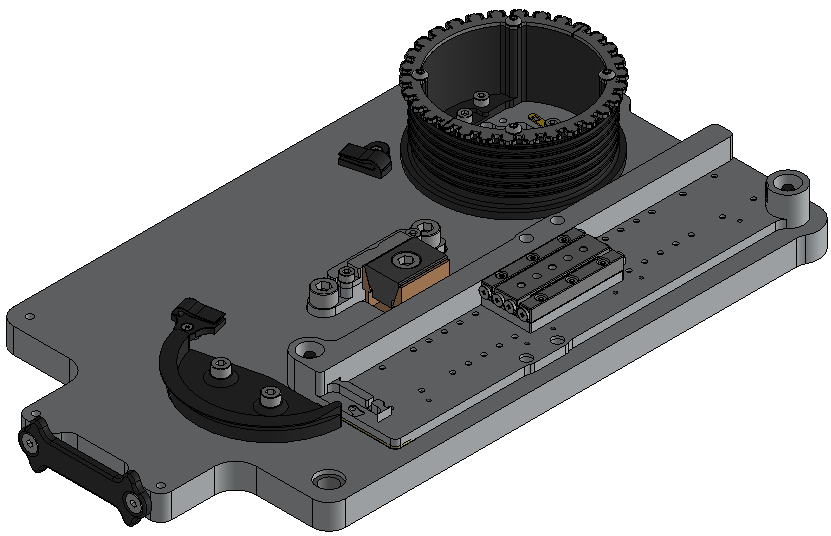
\includegraphics[width=0.5\linewidth]{Bilder/04_Konzeptentwicklung/Schnittstelle.png}
    \caption{Werkstückträger mit SLC2445}
    \label{fig:wst_slc2445}
\end{figure}

Elektrisch und informationstechnisch ergeben sich Schnittstellen zur Ansteuerung der Aktoren, zum Beispiel Achsen für die Schrauberpositionierung, die Schlittenbewegung und den Einpressvorgang. Zusätzlich müssen Sensoren eingebunden werden, um prozessrelevante Größen zu erfassen, insbesondere Drehmoment beim Schraubvorgang und – je nach Konzept – Kraft und Position beim Vorspannen. Die Steuerung muss diese Abläufe koordinieren und Messdaten so bereitstellen, dass die Funktionsweise des Systems im Rahmen von Tests nachvollziehbar überprüft werden kann.

Auf der Mensch-Maschine-Ebene bleibt das Be- und Entladen in der betrachteten Ausbaustufe manuell. Daraus ergibt sich die Anforderung an eine einfache Bedienung mit klaren Funktionen (Start, Stopp, Referenzieren, Quittieren) und einer verständlichen Status- und Fehlerrückmeldung.

\subsubsection{Anforderungsliste}
Die Anforderungen wurden aus der Aufgabenstellung, der Analyse des aktuellen Montageprozesses und den Randbedingungen der Fertigung abgeleitet. Zur besseren Übersicht sind sie in funktionale, mechanische, steuerungstechnische sowie sicherheits- und umgebungsbezogene Anforderungen gegliedert. Zusätzlich wurden sie nach Priorität in MUSS-, SOLL- und KANN-Kriterien eingeteilt. MUSS-Anforderungen dürfen vom späteren Konzept nicht verletzt werden, während SOLL-Anforderungen als Zielwerte dienen und KANN-Anforderungen optionale Verbesserungen darstellen.

Tabelle~\ref{tab:anforderungen_kurz} enthält die für die Konzeptentwicklung relevanten Anforderungen in kompakter Form. Die vollständige Anforderungsliste mit zusätzlichen Angaben (z. B. Nachweis, Kategorie und Kommentare) ist im Anhang~\ref{tab:anforderungsliste} dargestellt. Die Anforderungsliste wird in den folgenden Kapiteln als Grundlage für die Funktionsstruktur, die Bildung der Konzeptvarianten sowie die Bewertung in der Nutzwertanalyse verwendet.

Zur späteren Validierung wurden Anforderungen so formuliert, dass sie überprüfbar sind, z. B. über Maß- und Positionsmessungen, Drehmomentprotokolle oder Zykluszeitmessungen. Wo zum aktuellen Zeitpunkt noch keine konkreten Grenzwerte verfügbar sind, werden diese im Rahmen der konstruktiven Auslegung und der Versuche konkretisiert.\\

{
\small
\renewcommand{\arraystretch}{1.4}
\setlength{\tabcolsep}{12pt}

\begin{longtable}{|p{0.4cm}|p{8.0cm}|p{1.5cm}|p{2.0cm}|}
    \hline
        \textbf{ID} & \textbf{Anforderung (Kurzfassung)} & \textbf{Priorität} & \textbf{Zielwert} \\
    \hline
        \endfirsthead
        \endhead
    \hline
        \endfoot
        \endlastfoot
    
        A01 & Das System muss mit den vorhandenen Werkstückträgern (WST) kompatibel sein. & MUSS & -- \\
    \hline
        A02 & Das System muss die Baugrößen SLC-17 und SLC-24 verarbeiten können. & MUSS & -- \\
    \hline
        A03 & SLC-Positionierer mit Wand (SLC-W) müssen mittels Keile vorgespannt werden können. & MUSS & -- \\
    \hline
        A04 & SLC-Positionierer ohne Wand müssen mit dem bestehenden Vorspannsystem vorgespannt werden. & MUSS & -- \\
    \hline
        A05 & Das Vorspannsystem muss das Führungspaket parallel zur Referenzfläche ausrichten. & MUSS & $\le 20\,\mu\mathrm{m}$ \\
    \hline
        A06 & Die Schrauben sind mit einem vordefinierten Drehmoment anzuziehen. & MUSS & \qty{25}{Ncm} - \qty{60}{Ncm} \\
    \hline
        A26 & Die Positionierabweichung des Schraubwerkzeugs darf in jede Richtung nicht größer als $15\,\mu\mathrm{m}$ sein. & MUSS & $\le 15\,\mu\mathrm{m}$ \\
    \hline
        A11 & Die maximale Systemgröße darf $1200 \times 760\,\mathrm{mm}$ nicht überschreiten. & MUSS & $1200 \times 760\,\mathrm{mm}$ \\
    \hline
        A10 & Die Bearbeitungsdauer pro Positionierer soll unter 5 Minuten liegen. & SOLL & $< 5\,\mathrm{min}$ \\
    \hline
        A22 & Umrüstung zwischen SLC-17 / SLC-24 (mit/ohne Wand) soll schnell und werkzeuglos möglich sein. & SOLL & -- \\
    \hline
    
    \caption{Kernanforderungen für die Konzeptentwicklung}
    \label{tab:anforderungen_kurz}
\end{longtable}
}

\subsubsection{Anforderungserklärung}
Ein Teil der definierten Anforderungen ist nicht lediglich als optionale Verbesserung zu verstehen, sondern entscheidet maßgeblich darüber, ob das System im praktischen Einsatz zuverlässig funktioniert und reproduzierbare Ergebnisse liefert. Die nachfolgend erläuterten Anforderungen sind daher für die spätere Umsetzbarkeit und Bewertung des Konzepts von besonderer Bedeutung.

\begin{itemize}
    \item \textbf{WST-Kompatibilität (A01)} \\
    Die Kompatibilität mit den bestehenden Werkstückträgern stellt eine grundlegende Voraussetzung dar. Abweichungen würden unmittelbare Folgewirkungen nach sich ziehen, etwa Anpassungen an der Zuführung, zusätzliche Aufnahmen oder Umrüstungen in vorgelagerten Systemen. Solche Änderungen wären in der Fertigung nur schwer vermittelbar und würden den wirtschaftlichen Nutzen des Systems deutlich reduzieren. Aus diesem Grund ist diese Anforderung zwingend einzuhalten.

    \item \textbf{Variantenfähigkeit (A02–A04)} \\
    Die Baugrößen SLC-17 und SLC-24 sind als Produktvarianten fest vorgegeben. Zusätzlich stellt die Unterscheidung zwischen Ausführungen mit und ohne Wand unterschiedliche Anforderungen an den Vorspannprozess. Während bei SLC-W-Varianten Keile eingebracht werden müssen, ist bei den übrigen Varianten das bestehende Vorspannsystem zu berücksichtigen. Ein Konzept, das nur eine dieser Varianten abbilden kann, würde im Fertigungsalltag schnell zu einer Insellösung werden. Ziel ist daher eine möglichst flexible Lösung, die alle relevanten Varianten abdeckt.

    \item \textbf{Gleichmäßige Vorspannung (A05)} \\
    Die Einstellung der Vorspannung zählt zu den sensibelsten Schritten im aktuellen Montageprozess. Eine ungleichmäßige Vorspannung über die Führungslänge kann zu einer nicht parallelen Ausrichtung des Führungspakets führen, was lokal erhöhte Reibung oder Überlastungen verursacht und sich negativ auf das Laufverhalten sowie die Lebensdauer des Positionierers auswirkt.  
    Die Vorgabe einer maximalen Parallelitätsabweichung von \enquote{$\leq 20\,\mu\mathrm{m}$} über die gesamte Führungslänge stellt dabei ein eindeutiges und überprüfbares Qualitätskriterium dar.

    \item \textbf{Drehmoment beim Schrauben (A06)} \\
    Das beim Verschrauben eingebrachte Drehmoment steht in direktem Zusammenhang mit der resultierenden Klemmkraft. Schwankungen wirken sich somit unmittelbar auf die Gesamtqualität des Aufbaus aus. Gerade hier bietet eine teilautomatisierte Lösung klare Vorteile, da eine Überwachung und Dokumentation des Drehmoments möglich wird.

    \item \textbf{Positioniertoleranz des Schraubwerkzeugs (A26)} \\
    Die präzise Positionierung des Schraubwerkzeugs ist entscheidend für einen qualitativ hochwertigen Schraubprozess. Ungenaue Werkzeugführung kann zu Schrägansätzen, zusätzlichen Querkräften oder im ungünstigsten Fall zu beschädigten Schraubenköpfen oder Gewinden führen. Die Anforderung einer Positioniertoleranz von \enquote{$\leq 15\,\mu\mathrm{m}$ in alle Richtungen} verdeutlicht, dass es sich hierbei um einen Präzisionsschritt handelt, der dem Qualitätsniveau des Gesamtprodukts entsprechen muss.

    \item \textbf{Bauraum und Budget (A11, A13)} \\
    Die Begrenzung von Bauraum und Kosten definiert den zulässigen Lösungsraum für die Konzeptentwicklung. Der verfügbare Bauraum ist dabei durch die Abmessungen des vorgesehenen ITEM-Arbeitstisches festgelegt, auf dem das System montiert werden soll. Die nutzbare Tischfläche beträgt 1200\,mm $\times$ 760\,mm und stellt eine feste geometrische Randbedingung für den mechanischen Aufbau dar. Alle Baugruppen müssen innerhalb dieser Fläche angeordnet werden, sodass eine sichere Montage, Bedienbarkeit und Integration in die bestehende Fertigungsumgebung gewährleistet sind.\\Zusätzlich begrenzt das zur Verfügung stehende Budget die Auswahl von Komponenten und Lösungsprinzipien. Beide Randbedingungen müssen bereits in einer frühen Phase der Konzeptentwicklung berücksichtigt werden, um technisch realisierbare, wirtschaftlich sinnvolle und in die Fertigung integrierbare Lösungen zu gewährleisten.

    \item \textbf{Prozessdaten und Testskripte (A09, A12)} \\
    Für die Validierung des Systems sowie für eine objektive Bewertung der Prozessstabilität sind geeignete Prozessdaten erforderlich. Ergänzend ermöglichen automatisierte Testskripte eine strukturierte Überprüfung der Steuerungsabläufe und erhöhen die Nachvollziehbarkeit der Ergebnisse. Diese Anforderungen tragen dazu bei, das System nicht nur mechanisch, sondern ganzheitlich zu betrachten.

    \item \textbf{Zykluszeit (A10)} \\
    Die geforderte Zykluszeit von unter fünf Minuten stellt ein sinnvolles Ziel dar, ist jedoch stark vom Automatisierungsgrad und dem verbleibenden manuellen Handling abhängig. Als Soll-Kriterium ist sie realistisch angesetzt und erlaubt es, Qualitäts- und Prozesssicherheitsanforderungen höher zu gewichten, ohne das Gesamtkonzept grundsätzlich infrage zu stellen.
\end{itemize}

\subsection{Funktionsstruktur des Systems}
Ziel der Funktionsstruktur ist es, die Gesamtaufgabe des Systems unabhängig von einer konkreten konstruktiven Lösung zu beschreiben. Durch die Zerlegung in Teilfunktionen wird transparent, welche Funktionen das System erfüllen muss und wie diese logisch miteinander verknüpft sind. Die Funktionsstruktur bildet damit die Grundlage für die nachfolgende Konzeptentwicklung und -bewertung.

\subsubsection{Gesamtfunktion}
Die Gesamtfunktion des Systems besteht darin, Linearführungen der SLC-Positionierer reproduzierbar und qualitätsgesichert zu montieren. Dies umfasst das kontrollierte Vorspannen des Führungspakets, das präzise Verschrauben sowie die Handhabung unterschiedlicher Produktvarianten. Der Prozess soll dabei kompatibel zu bestehenden Werkstückträgern sein, prozessrelevante Daten erfassen und unter definierten Sicherheits- und Randbedingungen ablaufen.\\
Zusammenfassend lässt sich die Gesamtfunktion wie folgt formulieren:
\begin{quote}
\textit{Vorspannen und Verschrauben von SLC-Linearführungen unter kontrollierten Kraft-, Positions- und Drehmomentbedingungen bei gleichzeitiger Variantenfähigkeit und Prozessüberwachung.}
\end{quote}

\subsubsection{Funktionszerlegung}
Zur funktionalen Beschreibung des Systems wird die Gesamtfunktion in übergeordnete Teilfunktionen zerlegt. Ziel dieser Zerlegung ist es, die wesentlichen Aufgaben des Systems strukturiert darzustellen, ohne bereits auf konkrete technische Lösungen einzugehen.

Die Funktionszerlegung orientiert sich am grundsätzlichen Montageablauf der Linearführungen sowie an den identifizierten, qualitätsrelevanten Prozessschritten. Dabei wird zwischen vorbereitenden Funktionen, montagebezogenen Kernfunktionen und abschließenden Funktionen unterschieden.

Der Prozess beginnt mit dem Einlegen und Erkennen des Werkstückträgers. Anschließend erfolgt eine variantenabhängige Vorspannung des Führungspakets, gefolgt vom positionsgenauen Schraubprozess. Nach Abschluss der Montage wird der Werkstückträger entnommen.

Entscheidungen, insbesondere die Unterscheidung zwischen SLC- und SLC-W-Varianten, sind als funktionale Verzweigungen berücksichtigt. Wiederkehrende Abläufe, wie das schrittweise Verschrauben entlang der Führung, werden funktional als Schleifen abgebildet.

Die detaillierte Betrachtung und Bewertung der einzelnen Teilfunktionen erfolgt im Abschnitt~\ref{sec:teilfunktionen}.

\subsubsection{System- und Funktionsstrukturdiagramm}
Der Montageprozess der Linearführung lässt sich als eine klar strukturierte Abfolge einzelner Arbeitsschritte beschreiben. Um diesen Ablauf nachvollziehbar darzustellen, wird ein Funktionsstrukturdiagramm in Form eines Ablaufdiagramms verwendet. Es zeigt den Prozess vom Einlegen des Werkstückträgers bis zur Entnahme des montierten Bauteils.

Der Ablauf folgt der tatsächlichen Reihenfolge der Montage. Entscheidungen, wie die Unterscheidung zwischen SLC- und SLC-W-Varianten, sind als Verzweigungen im Diagramm integriert. Dadurch kann der gleiche grundlegende Ablauf für beide Produktvarianten verwendet werden, ohne separate Prozesse darstellen zu müssen.

Arbeitsschritte, die mehrfach durchlaufen werden, sind als Schleifen ausgeführt. Dies betrifft insbesondere das Einschrauben der Befestigungsschrauben und das anschließende Verschieben des Schlittens, bis alle Schrauben vollständig eingeschraubt sind. Auf diese Weise wird der sequentielle Charakter des Montageprozesses klar erkennbar.

Das Funktionsstrukturdiagramm dient damit als Übersicht über den zeitlichen und logischen Ablauf des Montageprozesses und bildet die Grundlage für die weitere funktionale Betrachtung des Systems.

\begin{figure}[htbp]
    \centering
    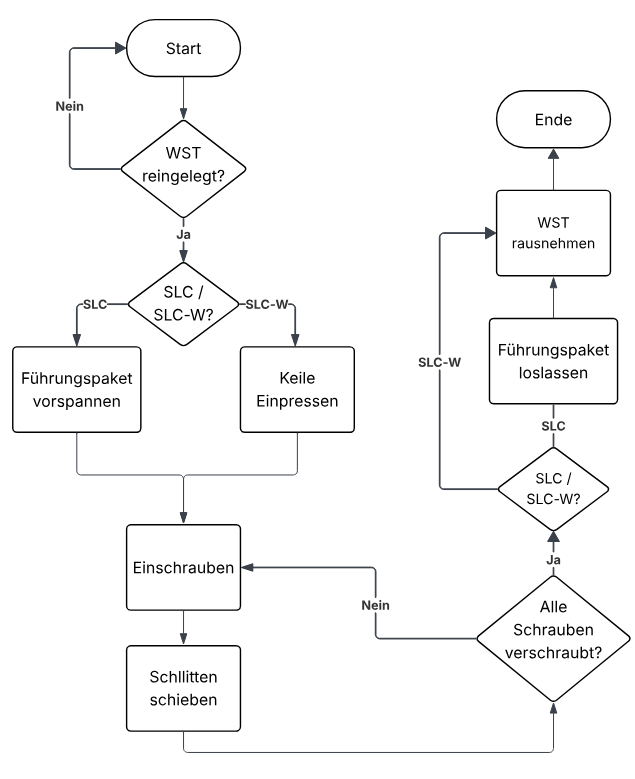
\includegraphics[width=0.48\linewidth]{Bilder/04_Konzeptentwicklung/Flowchart.png}
    \caption{Ablaufsdiagramm des Montageprozesses}
    \label{fig:Flowchart}
\end{figure}

\subsubsection{Strukturelle Funktionsstruktur der Montagesystems}

Neben dem zeitlichen Ablauf ist es für das Verständnis des Systems notwendig, die Montagestation als funktionale Einheit zu betrachten. Zu diesem Zweck wird eine strukturelle Funktionsstruktur verwendet, die das System unabhängig vom zeitlichen Ablauf beschreibt.

In dieser Darstellung ist die Montagestation als abgegrenztes System dargestellt, das mit seiner Umgebung über definierte Ein- und Ausgänge verbunden ist. Innerhalb der Systemgrenze sind die wesentlichen Funktionen zusammengefasst, die zur Umsetzung des Montageprozesses erforderlich sind. Dazu zählen unter anderem das Positionieren und Fixieren des Werkstückträgers, das Vorspannen beziehungsweise Einpressen des Führungspakets, der Schraubprozess sowie die Überwachung und Freigabe einzelner Prozessschritte.

Die strukturelle Funktionsstruktur macht deutlich, welche Funktionen im System realisiert werden und wie diese gemeinsam zur Erfüllung der Gesamtfunktion beitragen. Im Gegensatz zum Ablaufdiagramm wird hier bewusst keine zeitliche Reihenfolge dargestellt. Stattdessen liegt der Fokus auf der funktionalen Gliederung des Systems und der Abgrenzung zur Umgebung.

Die strukturelle Funktionsstruktur stellt damit die Verbindung zwischen dem Ablaufdiagramm und der anschließenden Betrachtung der Informations- und Energieflüsse dar.

\begin{figure}[htbp]
    \centering
    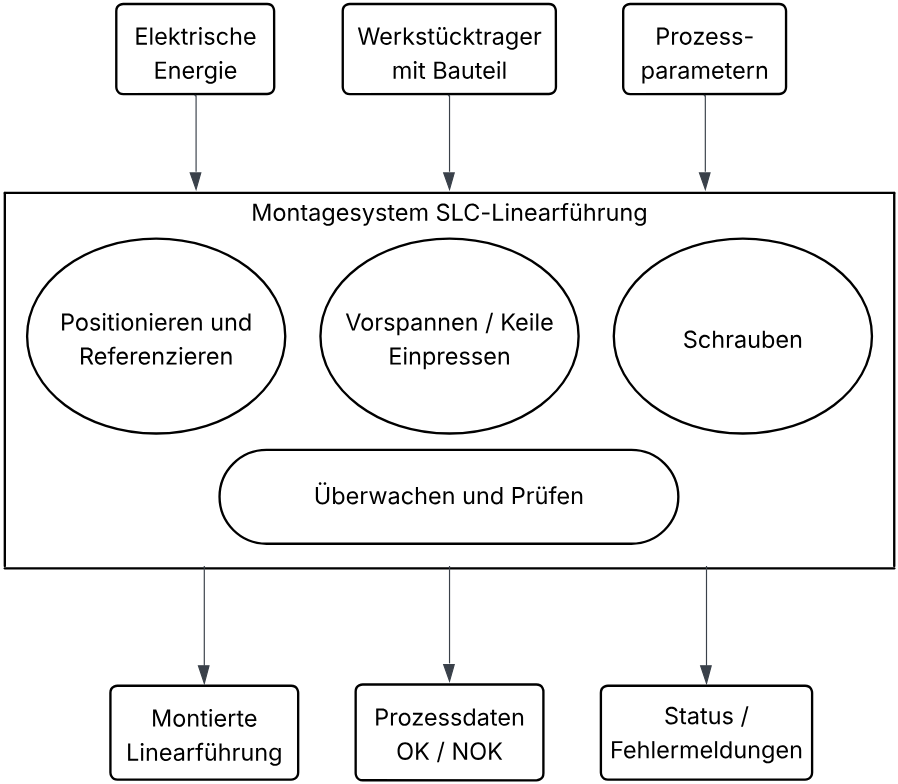
\includegraphics[width=0.45\linewidth]{Bilder/04_Konzeptentwicklung/Strukturelle Funktionsdiagramm.png}
    \caption{Strukturelle Funktionsstruktur des Montagesystems}
    \label{fig:Strukturelle_Funktionsstruktur}
\end{figure}

Die Funktionsstruktur bildet damit die Grundlage für die nachfolgende Konzeptentwicklung und -bewertung.\cite{VDI2221, MKon_VL, PahlBeitz}

\subsection{Lösungsprinzipien und Konzeptvarianten}
\subsubsection{Teilfunktionen}
\label{sec:teilfunktionen}
Aufbauend auf der im vorherigen Abschnitt dargestellten Funktionsstruktur werden im Folgenden die für die Konzeptentwicklung relevanten Teilfunktionen betrachtet. Ziel dieses Abschnitts ist es, diese Teilfunktionen eindeutig zu benennen und voneinander abzugrenzen, sodass sie im weiteren Verlauf gezielt als Grundlage für die Entwicklung technischer Lösungsprinzipien genutzt werden können.

Während die Funktionsstruktur die Aufgaben des Systems bewusst lösungsneutral beschreibt, stellen die Teilfunktionen die Verbindung zwischen der funktionalen Analyse und der späteren technischen Umsetzung dar. Sie konkretisieren die funktionalen Anforderungen soweit, dass darauf aufbauend unterschiedliche Lösungsansätze systematisch entwickelt, verglichen und kombiniert werden können.\cite{VDI2221, MKon_VL}

Die Identifikation der Teilfunktionen erfolgte auf Basis des realen Montageablaufs sowie der zuvor abgeleiteten Anforderungen. Der Schwerpunkt liegt dabei auf den qualitätskritischen Prozessschritten beim Aufbau der Linearführungen. Insbesondere die reproduzierbare Vorspannung des Führungspakets, der kontrollierte Schraubprozess sowie die übergeordnete Steuerung und Prozessüberwachung stehen im Fokus der Betrachtung.

Zur besseren Übersicht sind die identifizierten Haupt-, Unter- und Teilfunktionen in Tabelle~\ref{tab:teilfunktionen} strukturiert zusammengefasst. Zusätzlich ist der Bezug zu den jeweiligen Anforderungen angegeben. Die Tabelle dient als funktionale Orientierung für die nachfolgende Konzeptentwicklung und ermöglicht eine klare Zuordnung der späteren Lösungsprinzipien zu den einzelnen Teilfunktionen. Die inhaltliche Erläuterung der wesentlichen Teilfunktionen erfolgt im Anschluss.

{
\small
\setlength{\tabcolsep}{6pt}
\renewcommand{\arraystretch}{1.2}

\begin{longtable}{|p{0.5cm}|p{2.5cm}|p{0.6cm}|p{3.5cm}|p{0.8cm}|p{5.0cm}|}
\hline
\textbf{Nr.} & \textbf{Hauptfunktion} &
\textbf{Nr.} & \textbf{Unterfunktion} &
\textbf{Nr.} & \textbf{Teilfunktion} \\
\hline
\endfirsthead
\endhead
\hline
\endfoot
\endlastfoot

1 & Führungspaket vorspannen (SLC) & 1.1 & Werkstückaufnahme &
1.1.1 & Kompatibilität mit Werkstückträgern sicherstellen (A01) \\
\cline{3-6}
  &  & 1.2 & Baugrößenerkennung &
1.2.1 & SLC-17 / SLC-24 erkennen und umstellen (A02) \\
\cline{3-6}
  &  & 1.3 & Vorspannkraft einbringen &
1.3.1 & Gleichmäßige Vorspannung über die Länge sicherstellen (A05) \\
\cline{3-6}
  &  & 1.4 & Maßhaltigkeit sichern &
1.4.1 & Toleranzen beim Führungseinbau einhalten (A13) \\
\hline

2 & Einklappfedern einpressen (SLC-W) & 2.1 & Federvorspannung erzeugen &
2.1.1 & Einklappfedern bei SLC mit Wand einpressen (A03) \\
\cline{3-6}
  &  & 2.2 & Positionierung des Feder-Drückteils &
2.2.1 & Feder-Drückteil definiert zur Einklappfeder ausrichten und positionieren (A04) \\
\hline

3 & Schraubprozess & 3.1 & Schrauben eindrehen &
3.1.1 & Schrauben mit definiertem Drehmoment anziehen (A06) \\
\cline{3-6}
  &  & 3.2 & Werkzeugführung &
3.2.1 & Schraubwerkzeug präzise positionieren (A07) \\
\hline

4 & Steuerung und Prozessüberwachung & 4.1 & Montageablauf steuern &
4.1.1 & Steuerung aus Hardware und Software auswählen und implementieren (A08) \\
\cline{3-6}
  &  & 4.2 & Steuerungsvalidierung &
4.2.1 & Testskripte entwickeln und Abläufe prüfen (A09) \\
\cline{3-6}
  &  & 4.3 & Prozessüberwachung &
4.3.1 & Positions-, Drehmoment- und Prozessdaten erfassen (A11, A15) \\
\cline{3-6}
  &  & 4.4 & Bedien- und Umrüstschnittstelle &
4.4.1 & Umrüstung zwischen SLC-17 und SLC-24 ermöglichen (A21) \\
\cline{3-6}
  &  & 4.5 & Sollzeitgerechte Auslegung &
4.5.1 & Einhaltung der Soll-Bearbeitungszeit (A25) \\
\hline

5 & Wartung und Erweiterbarkeit & 5.1 & Wartungsfreundlichkeit &
5.1.1 & Wartungsarm gestalten (A19) \\
\cline{3-6}
  &  & 5.2 & Erweiterbarkeit &
5.2.1 & System für neue Baugrößen vorbereiten (A20) \\
\hline

6 & Optionale Systemmerkmale & 6.1 & Energieeffizienz &
6.1.1 & Energieverbrauch optimieren (A23) \\
\cline{3-6}
  &  & 6.2 & Transportfähigkeit &
6.2.1 & System auf Rollen oder modular zerlegbar gestalten (A24) \\
\hline

\caption{Übersicht der Haupt-, Unter- und Teilfunktionen des Montagesystems}
\label{tab:teilfunktionen}
\end{longtable}
}

\begin{enumerate}
    \item \textbf{Führungspaket vorspannen}\\
    Ziel dieser Hauptfunktion ist es, eine definierte und reproduzierbare Vorspannung über die gesamte Länge der Linearführung sicherzustellen.

    Hierfür sind insbesondere folgende Teilfunktionen erforderlich:
    \begin{itemize}
        \item \textbf{Gleichmäßige Vorspannkraft erzeugen}\\
        Sicherstellung einer gleichmäßigen Kraftverteilung entlang der Führung, um eine parallele Ausrichtung des Führungspakets zur Referenzfläche zu gewährleisten.

        \item \textbf{Vorspannelement in Richtung SLC bewegen}\\
        Gezielte, geführte Bewegung eines Vorspannelements zur kontrollierten Einbringung der erforderlichen Vorspannkraft.

        \item \textbf{Einklappfedern einpressen (SLC-W)}\\
        Variantenabhängige Erzeugung der Vorspannung durch das kontrollierte Einpressen der Einklappfedern bei SLC-Positionierern mit Wand.
        \begin{itemize}
            \item \textbf{Position der Feder erfassen}\\
            Überwachung der Lage der Einklappfeder während des Einpressvorgangs.
            \item \textbf{Einpresskraft einstellen}\\
            Anpassung der Einpresskraft zur Vermeidung von Beschädigungen und zur Sicherstellung reproduzierbarer Ergebnisse.
        \end{itemize}
    \end{itemize}
    
    \item \textbf{Schraubprozess}\\
    Der Schraubprozess dient der form- und kraftschlüssigen Fixierung der Linearführung in der vorgespannten Position. Die Prozessqualität hängt dabei wesentlich von der präzisen Positionierung des Schraubwerkzeugs sowie von der kontrollierten Einbringung des Drehmoments ab.

    Die hierfür relevanten Teilfunktionen sind:
    \begin{itemize}
        \item \textbf{Position der Schrauben erfassen}\\
        Bestimmung der jeweiligen Schraubpositionen als Grundlage für eine präzise Werkzeugführung.

        \item \textbf{Schraubwerkzeug positionieren}\\
        Exaktes Anfahren der Schraubpositionen innerhalb der vorgegebenen Toleranzen.

        \item \textbf{Drehmoment einstellen und überwachen}\\
        Sicherstellung eines definierten Drehmoments während des Einschraubvorgangs.

        \item \textbf{Schraubtiefe erfassen}\\
        Kontrolle der Einschraubtiefe als zusätzliches Qualitätsmerkmal.

        \item \textbf{Schlitten schieben}\\
        Inkrementelle Bewegung des Schlittens entlang der Führung, um den Schraubprozess schrittweise über die gesamte Führungslänge durchführen zu können.
    \end{itemize}

    \item \textbf{Steuerung und Prozessüberwachung}\\
    Die Steuerung koordiniert alle Teilfunktionen und stellt sicher, dass der Montageprozess in der vorgesehenen Reihenfolge und unter Einhaltung der definierten Randbedingungen abläuft. Zusätzlich übernimmt sie Aufgaben der Prozessüberwachung sowie der Datenerfassung.

    Zentrale Teilfunktionen in diesem Bereich sind:
    \begin{itemize}
        \item \textbf{Subsysteme kalibrieren}\\
        Kalibrierung von Sensoren und Referenzierung von Aktoren zur Sicherstellung reproduzierbarer Prozessbedingungen.

        \item \textbf{Montageprozess steuern}\\
        Ablaufsteuerung der einzelnen Prozessschritte einschließlich Variantenentscheidung und Fehlerbehandlung.
    \end{itemize}
\end{enumerate}

\textbf{Zusammenfassung und Überleitung}\\
Die beschriebenen Teilfunktionen bilden die funktionale Grundlage für die nachfolgende Entwicklung technischer Lösungsprinzipien. In den folgenden Abschnitten werden für ausgewählte Teilfunktionen unterschiedliche Lösungsansätze untersucht und zu konsistenten Konzeptvarianten zusammengeführt.

\subsubsection{Lösungsprinzipien für Teilfunktionen}
\label{sec:teilfuktionenlösungen}
Für die in Abschnitt~\ref{sec:teilfunktionen} definierten Teilfunktionen wurden jeweils mehrere technische Lösungsprinzipien identifiziert. Ziel dieses Abschnitts ist es, die möglichen Umsetzungsansätze pro Teilfunktion übersichtlich darzustellen, ohne diese bereits zu einem Gesamtkonzept zu kombinieren oder zu bewerten.\cite{MKon_VL, PahlBeitz, ZwickyMorphology}

Die Lösungsprinzipien wurden auf der Basis des bestehenden Montageprozesses, der technischen Machbarkeit sowie der definierten Anforderungen erarbeitet. Dabei wurden sowohl einfach ausgestaltete, robuste Lösungen als auch stärker automatisierte Ansätze berücksichtigt, um ein breites Lösungsspektrum abzudecken.

Für die Werkstückaufnahme wurden sowohl manuelle Einlegekonzepte als auch automatisierte Varianten, beispielsweise mittels eines 6-achsen-Roboters, betrachtet. Die Sicherung des Werkstücks kann mechanisch über Spannvorrichtungen mit Passstiften oder alternativ über Vakuumbasierte Systeme erfolgen.

Im Bereich der Baugrößenumschaltung reichen die Lösungsansätze von einer manuellen Eingabe über das automatische Einlesen eines Codes bis hin zu sensor- oder kamerabasierten Erkennungsverfahren. Das Vorspannsystem kann entweder auf einem bereits bestehenden mechanischen System aufbauen oder durch zusätzliche Aktorik ergänzt werden.

Zur Erfassung der Schlittenposition wurden verschiedene sensorische Prinzipien untersucht, darunter geführte Bewegungen bis zum Werkstückanschlag, Laser-Triangulations\-sensoren, kamerabasierte Systeme sowie ToF-Sensorik. Für die Bewegung des Schraubwerkzeugs wurden kartesische Systeme wie XYZ- oder Gantry-Achsen ebenso betrachtet wie robotische Lösungen mit höherer Bewegungsfreiheit.

Beim Einschraubsystem wurden sowohl einfache manuelle Schraubwerkzeuge als auch drehmomentgeregelte industrielle Schrauber untersucht. Ergänzend wurden unterschiedliche Konzepte für den Endeffektor, die Positionsüberwachung, das Steuerungssystem sowie Sicherheits-, Transport- und Energieeffizienzaspekte betrachtet.\\\\

{
\small
\setlength{\tabcolsep}{4pt}
\renewcommand{\arraystretch}{1.2}

\begin{tabularx}{\textwidth}{|p{3.5cm}|X|X|X|X|}
\hline
\textbf{Teilfunktion} & \multicolumn{4}{c|}{\textbf{Lösungsprinzipien}} \\
\hline
\endfirsthead
\endhead
\hline
\endfoot
\endlastfoot

WST-Aufnahme & Manuelle Einsetzung & Einsetzung durch Cobot & -- & -- \\
\hline
WST-Sicherung & Spannvorrichtung mit Stiften & Vakuum\-aufnahme & -- & -- \\
\hline
Baugrößen\-identifikation & Automatisches Code-Scannen & Manuelle Eingabe & Sensor- oder bildbasierte Erkennung & -- \\
\hline
Vorspannsystem & Bestehendes mechanisches Vorspannsystem & -- & -- & -- \\
\hline
Schlittenposition erfassen & Geführte Bewegung bis Werkstückanschlag & Laser-Triangulations- / IR-Sensor & Kamera & ToF-Sensor \\
\hline
Schrauber\-bewegungssystem & XYZ-Achsensystem & Gantry-System & 6-Achs-Roboter & SCARA / Pick-and-Place \\
\hline
Einklappfedern einpressen & Hydraulische Presse & Ventilgesteuerte Presse & Motor\-angetriebener Stift & -- \\
\hline
Einschraubsystem & Konventioneller Schraubendreher mit drehbarem Endeffektor & Drehmoment\-geregelter Schrauber (z.\,B. MITO15CA + EDU 2AE) & -- & -- \\
\hline
Schiebersystem & Aufsteckbares Gummipad mit manueller Presse & Gummiauflage auf Hülse & Gummistift & -- \\
\hline
Endeffektor & Einfacher Greifer & Kombinierter Endeffektor & Mehrfach-Endeffektor & -- \\
\hline
Positions\-überwachung & Encoder & Schrittzähler & Distanzsensoren & Bildverarbeitung \\
\hline
Steuerungssystem & SPS-basierte Steuerung & IPC-basiertes Motion-Control-System & Industrie-Robotercontroller & -- \\
\hline
Transportfähigkeit & Fix montiert & Rollen mit Feststeller & Modular zerlegbar & -- \\
\hline
Energieeffizienz & Intelligente Abschaltung bei Inaktivität & Keine Optimierung & Energiesparende Antriebe & -- \\
\hline

\caption{Übersicht der Lösungsprinzipien für die einzelnen Teilfunktionen}
\label{tab:loesungsprinzipien_teilfunktionen}
\end{tabularx}
}

Die Gesamtheit dieser Lösungsprinzipien ist im morphologischen Kasten strukturiert dargestellt und bildet die Grundlage für die nachfolgende Bildung von Konzeptvarianten.

\subsubsection{Bildung von Konzeptvarianten}
Zur Bildung konsistenter Gesamtkonzepte wurden die in Abschnitt~\ref{sec:teilfuktionenlösungen} dargestellten Lösungsprinzipien mithilfe eines morphologischen Kastens systematisch kombiniert. Der morphologische Kasten stellt für jede Teilfunktion mehrere alternative Lösungsansätze gegenüber und ermöglicht es, diese gezielt zu vollständigen Konzeptvarianten zusammenzuführen.

Eine Konzeptvariante entsteht dabei durch die Auswahl genau eines Lösungsprinzips pro Teilfunktion. Durch das Verbinden dieser ausgewählten Lösungen im morphologischen Kasten ergeben sich zusammenhängende Linien, die jeweils ein in sich geschlossenes Gesamtkonzept repräsentieren.

Bei der Auswahl der Kombinationen wurde darauf geachtet, dass die einzelnen Lösungsprinzipien technisch kompatibel sind und gemeinsam einen vollständigen Montageprozess abbilden. Gleichzeitig wurden bewusst unterschiedliche Automatisierungsgrade realisiert, um im weiteren Verlauf einen vergleichenden Ansatz zu ermöglichen.

Auf diese Weise wurden mehrere Konzeptvarianten definiert, die sich hinsichtlich Systemkomplexität, Automatisierungsgrad und technischer Ausprägung unterscheiden. Diese Varianten bilden die Grundlage für die nachfolgende detaillierte Beschreibung und Bewertung.
\\\\\\\\

\begin{center}
\small
\renewcommand{\arraystretch}{1.4}
\setlength{\tabcolsep}{12pt}
\begin{tabular}{|c|c|}
    \hline
    \textbf{Konzept} & \textbf{Linienmuster} \\
    \hline
    \textbf{A} &
    \textcolor{conceptA}{\rule{2.5cm}{0.8pt}} \\
    \hline
    \textbf{B} &
    \textcolor{conceptB}{
        \rule[0.3ex]{0.5cm}{0.8pt}\hspace{0.2cm}
        \rule[0.3ex]{0.5cm}{0.8pt}\hspace{0.2cm}
        \rule[0.3ex]{0.5cm}{0.8pt}
    } \\
    \hline
    \textbf{C} &
    \textcolor{conceptC}{
        \rule[0.3ex]{0.15cm}{0.8pt}\hspace{0.15cm}
        \rule[0.3ex]{0.15cm}{0.8pt}\hspace{0.15cm}
        \rule[0.3ex]{0.15cm}{0.8pt}\hspace{0.15cm}
        \rule[0.3ex]{0.15cm}{0.8pt}\hspace{0.15cm}
        \rule[0.3ex]{0.15cm}{0.8pt}\hspace{0.15cm}
        \rule[0.3ex]{0.15cm}{0.8pt}
    } \\
    \hline
\end{tabular}
\end{center}
\clearpage

\begin{comment}
{
\small
\setlength{\tabcolsep}{4pt}
\renewcommand{\arraystretch}{1.2}

\begin{tabularx}{\textwidth}{|p{3.5cm}|X|X|X|X|}
\hline
\textbf{Teilfunktion} & \multicolumn{4}{c|}{\textbf{Lösungsprinzipien}} \\
\hline

WST-Aufnahme
& Manuelle Einsetzung \cellnode{wst_man}
& Einsetzung durch Cobot \cellnode{wst_cobot}
& -- & -- \\
\hline

WST-Sicherung
& Spannvorrichtung mit Stiften \cellnode{sich_stift}
& Vakuum\-aufnahme \cellnode{sich_vak}
& -- & -- \\
\hline

Baugrößen\-identifikation
& Automatisches Code-Scannen \cellnode{id_code}
& Manuelle Eingabe \cellnode{id_man}
& Sensor- oder bildbasierte Erkennung \cellnode{id_cam}
& -- \\
\hline

Vorspannsystem
& Bestehendes mechanisches Vorspannsystem \cellnode{vorspann}
& -- & -- & -- \\
\hline

Schlittenposition erfassen
& Geführte Bewegung bis Werkstückanschlag \cellnode{pos_anschlag}
& Laser-Triangulations- / IR-Sensor \cellnode{pos_laser}
& Kamera \cellnode{pos_cam}
& ToF-Sensor \cellnode{pos_tof} \\
\hline

Schrauber\-bewegungssystem
& XYZ-Achsensystem \cellnode{move_xyz}
& Gantry-System \cellnode{move_gantry}
& 6-Achs-Roboter \cellnode{move_6ax}
& SCARA / Pick-and-Place \cellnode{move_scara} \\
\hline

Einklappfedern einpressen
& Hydraulische Presse \cellnode{press_hyd}
& Ventilgesteuerte Presse \cellnode{press_valve}
& Servo\-angetriebener Stift \cellnode{press_servo}
& -- \\
\hline

Einschraubsystem
& Konventioneller Schraubendreher \cellnode{screw_simple}
& Drehmoment\-geregelter Schrauber \cellnode{screw_mito}
& -- & -- \\
\hline

Schiebersystem
& Aufsteckbares Gummipad \cellnode{slide_pad}
& Gummiauflage auf Hülse \cellnode{slide_sleeve}
& Gummistift \cellnode{slide_pin}
& -- \\
\hline

Endeffektor
& Einfacher Greifer \cellnode{ee_simple}
& Kombinierter Endeffektor \cellnode{ee_combo}
& Mehrfach-Endeffektor \cellnode{ee_multi}
& -- \\
\hline

Positions\-überwachung
& Encoder \cellnode{ctrl_enc}
& Schrittzähler \cellnode{ctrl_step}
& Distanzsensoren \cellnode{ctrl_dist}
& Bildverarbeitung \cellnode{ctrl_img} \\
\hline

Steuerungssystem
& SPS-basierte Steuerung \cellnode{ctrl_plc}
& IPC-basiert \cellnode{ctrl_ipc}
& Robotercontroller \cellnode{ctrl_robot}
& -- \\
\hline

Transportfähigkeit
& Fix montiert
& Rollen mit Feststeller
& Modular zerlegbar
& -- \\
\hline

Energieeffizienz
& Intelligente Abschaltung
& Keine Optimierung
& Energiesparende Antriebe
& -- \\
\hline

\caption{Übersicht der Lösungsprinzipien für die einzelnen Teilfunktionen}
\label{tab:morphologischer_kasten}
\end{tabularx}
}

\begin{tikzpicture}[remember picture,overlay]

% Beispiel: gewählte Lösung (rot)
\draw[red, very thick]
  (wst_cobot) -- (sich_stift)
  -- (id_code)
  -- (vorspann)
  -- (pos_laser)
  -- (move_xyz)
  -- (press_servo)
  -- (screw_mito)
  -- (slide_pin)
  -- (ee_combo)
  -- (ctrl_enc)
  -- (ctrl_plc);

% Alternative Variante (grün gestrichelt)
\draw[green!60!black, dashed, very thick]
  (wst_man) -- (sich_vak)
  -- (id_cam)
  -- (pos_cam)
  -- (move_gantry)
  -- (press_valve);

\end{tikzpicture}
\end{comment}

\begin{table}[H]
\centering
\small
\setlength{\tabcolsep}{4pt}
\renewcommand{\arraystretch}{1.2}

\begin{tabularx}{\textwidth}{|p{3.5cm}|X|X|X|X|}
\hline
\textbf{Teilfunktion} & \multicolumn{4}{c|}{\textbf{Lösungsprinzipien}} \\
\hline

WST-Aufnahme 
& Manuelle Einsetzung \cellnode{1_man}
& Einsetzung durch Cobot \cellnode{1_auto}
& -- & -- \\
\hline

WST-Sicherung 
& Spannvorrichtung mit Stiften \cellnode{2_spann}
& Vakuum\-aufnahme \cellnode{2_vak}
& -- & -- \\
\hline

Baugrößen\-identifikation 
& Automatisches Code-Scannen \cellnode{3_code}
& Manuelle Eingabe \cellnode{3_man}
& Sensor- oder bildbasierte Erkennung \cellnode{3_sensor}
& -- \\
\hline

Vorspannsystem 
& Bestehendes mechanisches Vorspannsystem \cellnode{4_vorsp}
& -- & -- & -- \\
\hline

Schlittenposition erfassen 
& Geführte Bewegung bis Werkstückanschlag \cellnode{5_schlag}
& Laser-Triangulations- / IR-Sensor \cellnode{5_laser}
& Kamera \cellnode{5_cam}
& ToF-Sensor \cellnode{5_tof} \\
\hline

Schrauber\-bewegungssystem 
& XYZ-Achsensystem \cellnode{6_xyz}
& Gantry-System \cellnode{6_p50}
& 6-Achs-Roboter \cellnode{6_cobot}
& SCARA / Pick-and-Place \cellnode{6_scara} \\
\hline

Einklappfedern einpressen 
& Hydraulische Presse \cellnode{7_hydro}
& Ventilgesteuerte Presse \cellnode{7_ventil}
& Motor\-angetriebener Stift \cellnode{7_servo}
& -- \\
\hline

Einschraubsystem 
& Konventioneller Schraubendreher mit drehbarem Endeffektor \cellnode{8_konv}
& Drehmoment\-geregelter Schrauber (z.\,B. MITO15CA + EDU~2AE) \cellnode{8_kolver}
& -- & -- \\
\hline

Schiebersystem 
& Aufsteckbares Gummipad mit manueller Presse \cellnode{9_man}
& Gummiauflage auf Hülse \cellnode{9_huelse}
& Gummistift \cellnode{9_gummi}
& -- \\
\hline

Endeffektor 
& Einfacher Greifer \cellnode{10_greifer}
& Kombinierter Endeffektor \cellnode{10_kombi}
& Mehrfach-Endeffektor \cellnode{10_mehrfach}
& -- \\
\hline

Positions\-überwachung 
& Encoder \cellnode{11_enc}
& Schrittzähler \cellnode{11_step}
& Distanzsensoren \cellnode{11_sensor}
& Bildverarbeitung \cellnode{11_bv} \\
\hline

Steuerungssystem 
& SPS-basierte Steuerung \cellnode{12_sps}
& IPC-basiertes Motion-Control-System \cellnode{12_ipc}
& Industrie-Robotercontroller \cellnode{12_ind}
& -- \\
\hline

Transportfähigkeit 
& Fix montiert \cellnode{13_fix}
& Rollen mit Feststeller \cellnode{13_rollen}
& Modular zerlegbar \cellnode{13_modular}
& -- \\
\hline

Energieeffizienz 
& Intelligente Abschaltung bei Inaktivität \cellnode{14_absch}
& Keine Optimierung \cellnode{14_nix}
& Energiesparende Antriebe \cellnode{14_spar}
& -- \\
\hline

\end{tabularx}

\caption{Übersicht der Lösungsprinzipien für die einzelnen Teilfunktionen}
\label{tab:morphologischer_kasten}
\end{table}

% ---- TikZ overlay (MUST be immediately after the table)
\begin{tikzpicture}[remember picture,overlay]
  \draw[red, very thick]
  ($(1_man)+(0,2.2mm)$)
  -- ($(2_spann)+(0,2.2mm)$)
  -- ($(3_man)+(0,2.2mm)$)
  -- ($(4_vorsp)+(0,2.2mm)$)
  -- ($(5_laser)+(0,2.2mm)$)
  -- ($(6_xyz)+(0,2.2mm)$)
  -- ($(7_servo)+(0,2.2mm)$)
  -- ($(8_kolver)+(0,2.2mm)$)
  -- ($(9_huelse)+(0,2.2mm)$)
  -- ($(10_kombi)+(0,2.2mm)$)
  -- ($(11_step)+(0,2.2mm)$)
  -- ($(12_ipc)+(0,2.2mm)$)
  -- ($(13_rollen)+(0,2.2mm)$)
  -- ($(14_nix)+(0,2.2mm)$);


  \draw[green!60!black, dashed, very thick]
  (1_man) -- (2_vak) -- (3_sensor) -- (4_vorsp) -- (5_cam) -- (6_p50) -- (7_ventil) -- (8_kolver) -- (9_gummi) -- (10_mehrfach) -- (11_bv) -- (12_ipc) -- (13_fix) -- (14_absch);

  \draw[blue, dotted, very thick]
  ($(1_man)+(0,-2.2mm)$)
  -- ($(2_spann)+(0,-2.2mm)$)
  -- ($(3_code)+(0,-2.2mm)$)
  -- ($(4_vorsp)+(0,-2.2mm)$)
  -- ($(5_laser)+(0,-2.2mm)$)
  -- ($(6_scara)+(0,-2.2mm)$)
  -- ($(7_servo)+(0,-2.2mm)$)
  -- ($(8_kolver)+(0,-2.2mm)$)
  -- ($(9_gummi)+(0,-2.2mm)$)
  -- ($(10_greifer)+(0,-2.2mm)$)
  -- ($(11_enc)+(0,-2.2mm)$)
  -- ($(12_ind)+(0,-2.2mm)$)
  -- ($(13_modular)+(0,-2.2mm)$)
  -- ($(14_spar)+(0,-2.2mm)$);

\end{tikzpicture}


\clearpage

\subsubsection{Beschreibung der Konzeptvarianten}

Im Folgenden werden die gebildeten Konzeptvarianten hinsichtlich ihrer wesentlichen Merkmale beschrieben. Der Fokus liegt dabei auf den charakteristischen Besonderheiten der jeweiligen Variante sowie auf den daraus resultierenden Vor- und Nachteilen. Eine quantitative Bewertung erfolgt erst im anschließenden Abschnitt.

\paragraph{Konzeptvariante A:}
Konzeptvariante A verfolgt einen bewusst einfach gehaltenen Ansatz mit geringem Automatisierungsgrad. Der Fokus liegt auf einem robusten, übersichtlichen Systemaufbau unter Nutzung weitgehend manueller oder bewährter technischer Lösungen. Ziel ist eine hohe Prozessstabilität bei gleichzeitig geringem Integrations- und Inbetriebnahmeaufwand.

Die Werkstückaufnahme erfolgt durch manuelle Einsetzung, während die Fixierung über eine pneumatische Spannvorrichtung realisiert wird. Die Baugrößenumschaltung erfolgt ebenfalls manuell. Für die Einstellung der Vorspannung wird das bereits bestehende Vorspannsystem verwendet.

Die Erfassung der Schlittenposition erfolgt mittels eines Laser-Triangulationssensors. Die Bewegung des Schraubwerkzeugs wird über ein kartesisches XYZ-Achsensystem umgesetzt. Das Einschrauben der Schrauben erfolgt mit einem drehmomentgeregelten Schrauber (MITO 15CA in Kombination mit EDU 2AE von Kolver). Um den Schlitten zu bewegen, kommt ein pneumatischer Kolbenstangenzylinder mit Gummikappe zum Einsatz. Als Endeffektor wird eine kombinierte Ausführung verwendet, die mehrere Funktionen integriert, zum Beispiel das Einschrauben, Einpressen der Keile und die Bewegung des Schlittens.

Die Steuerung basiert auf einem IPC-basierten Motion-Control-System. Die Station ist über Rollen mit Feststellern verfahrbar, und eine explizite Energieoptimierung ist in dieser Variante nicht vorgesehen.

\begin{figure}[htbp]
    \centering
    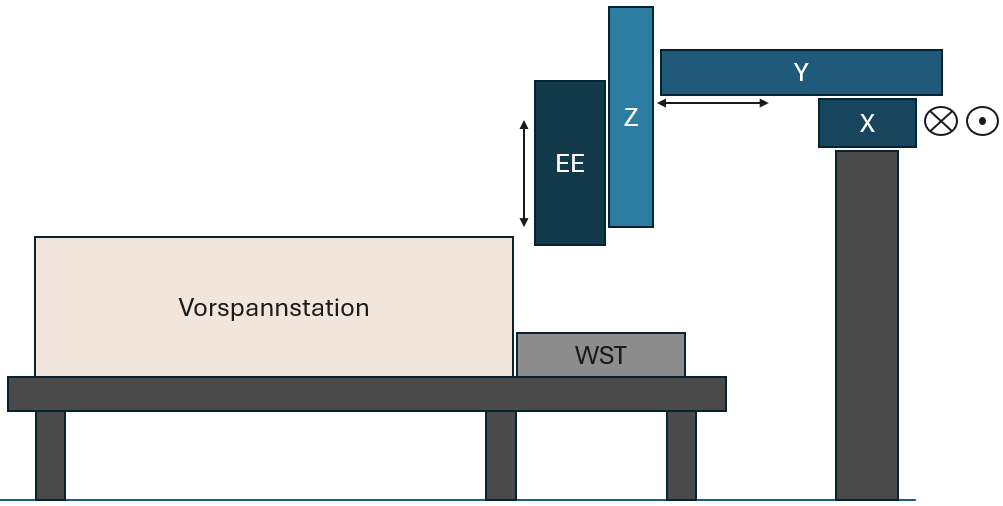
\includegraphics[width=0.8\linewidth]{Bilder/04_Konzeptentwicklung/Konzept_A.png}
    \caption{Zeichnung der Konzept A}
    \label{fig:concept_a}
\end{figure}

\textbf{Besonderheiten:}
\begin{itemize}
    \item Kartesische XYZ-Kinematik mit feststehender Vorspannstation
    \item Zugriff des Endeffektors von oben bzw. seitlich
    \item Klare Trennung zwischen Struktur, Kinematik und Prozessmodul
    \item Modularer Aufbau mit eindeutig definierten Achsen
\end{itemize}

\textbf{Vorteile:}
\begin{itemize}
    \item Hohe Positioniergenauigkeit durch einfache kartesische Bewegungen
    \item Gute Reproduzierbarkeit der Vorspann- und Schraubprozesse
    \item Hoher Automatisierungsgrad möglich
    \item Einfache Integration von Sensorik und Werkzeugen
    \item Hohe Wartungs- und Diagnosefreundlichkeit durch modularen Aufbau mit klar abgegrenzten, funktionsspezifischen Baugruppen
\end{itemize}

\textbf{Nachteile:}
\begin{itemize}
    \item Relativ hoher Platzbedarf, insbesondere in Z-Richtung
    \item Höherer konstruktiver Aufwand für ausreichende Steifigkeit
\end{itemize}

\paragraph{Konzeptvariante B:}
Konzeptvariante B stellt einen Kompromiss zwischen einem erhöhten Automatisierungsgrad und einer noch beherrschbaren Systemkomplexität dar.

Für diese Variante ist der Einsatz der P-50-Montageanlage der SmarAct Automation vorgesehen. Diese Anlage bietet einen hohen Integrationsgrad sowie einen hochpräzisen Gantry-Linearantrieb.\cite{SmarActAutomation_P50} Die Werkstückaufnahme erfolgt weiterhin manuell, während die Sicherung des Werkstücks über eine vakuumbasierte Aufnahme realisiert wird. Das Vorspannsystem basiert auch hier auf dem bereits bestehenden mechanischen System.

Die Erfassung der Schlittenposition erfolgt kamerabasiert, wodurch eine flexible und berührungslose Positionsbestimmung ermöglicht wird. Die Bewegung des Schraubwerkzeugs wird über ein Gantry-System umgesetzt. Das Einpressen der Einklappfedern erfolgt mittels einer ventilgesteuerten Presse. Der Schraubprozess wird mit einem drehmomentgeregelten MITO-Schrauber realisiert. Für Schiebebewegungen kommt ein Stift mit Gummiabdeckung zum Einsatz.

Als Endeffektor wird eine Mehrfach-Endeffektorlösung verwendet. Die Positionsüberwachung erfolgt über Encoder. Die Steuerung basiert auf einem IPC-basierten System. Die Station ist rollbar ausgeführt und verfügt über eine intelligente Abschaltung zur Reduzierung des Energieverbrauchs in Stillstandszeiten.

Im Vergleich zu Konzept A ist der technische Funktionsumfang deutlich erweitert. Gleichzeitig ist der Einsatz der P-50-Anlage mit einem erheblichen Investitionsaufwand verbunden, was diese Variante insbesondere aus wirtschaftlicher Sicht kritisch macht.

\begin{figure}[htbp]
    \centering
    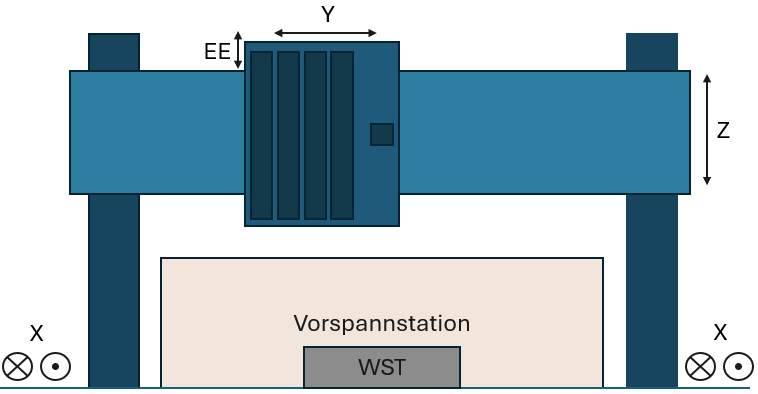
\includegraphics[width=0.8\linewidth]{Bilder/04_Konzeptentwicklung/Konzept_B.png}
    \caption{Zeichnung der Konzept B}
    \label{fig:concept_b}
\end{figure}

\textbf{Besonderheiten:}
\begin{itemize}
    \item Brückenförmiger Aufbau mit verfahrbarem Querträger
    \item Vorspannstation vollständig frei und stationär
    \item Kartesische Kinematik mit großem nutzbaren Arbeitsraum
    \item Zugriff von oben auf den Prozess
    \item Einsatz einer bestehenden Automationsplattform (P-50 aus SmarAct Automation) vorgesehen
\end{itemize}

\textbf{Vorteile:}
\begin{itemize}
    \item Deutlich reduzierter Konstruktions- und Entwicklungsaufwand durch die Nutzung einer vorhandenen Automationsanlage
    \item Hohe Integrationssicherheit durch erprobte Hardware und bestehende Schnittstellen
    \item Gute Eignung für teil- oder vollautomatisierte Prozesse
\end{itemize}

\textbf{Nachteile:}
\begin{itemize}
    \item Hoher Platzbedarf in der Fläche
    \item Sehr hohe Investitionskosten durch die Verwendung der SmarAct Automation P-50
    \item Wirtschaftlich nur bedingt sinnvoll für kleine Stückzahlen
    \item Geringere Freiheitsgrade bei der mechanischen Anpassung im Vergleich zu einer Eigenkonstruktion
\end{itemize}

\paragraph{Konzeptvariante C:}
Konzeptvariante C verfolgt einen deutlich stärkeren automatisierten und modularen Ansatz. Ziel ist eine hohe Flexibilität und Zukunftssicherheit, auch bei erhöhtem technischem und organisatorischem Aufwand.

Die Werkstückaufnahme erfolgt manuell, und die Sicherung erfolgt über eine mechanische Spannvorrichtung. Die Baugrößenumschaltung wird automatisch durch das Einlesen eines Data-Matrix-Codes realisiert. Für die Vorspannung wird weiterhin das bestehende mechanische Vorspannsystem verwendet.

Die Schlittenposition wird mittels eines Laser-Triangulationssensors erfasst. Die Bewegung des Schraubwerkzeugs erfolgt über ein Pick-and-Place-System. Das Einpressen der Einklappfedern wird durch eine servogetriebene Mini-Presse umgesetzt. Der Schraubprozess erfolgt auch hier mit einem drehmomentgeregelten MITO-Schrauber. Für Schiebebewegungen wird ein aufsteckbares Gummipad an der Presse eingesetzt.

Als Endeffektor kommt ein einfacher Greifer zum Einsatz. Die Positionsüberwachung erfolgt über Encoder. Die Steuerung basiert auf einem Industrie-Robotercontroller. Die Station ist modular zerlegbar ausgeführt und verfügt über eine intelligente Abschaltung zur Verbesserung der Energieeffizienz.

\begin{figure}[htbp]
    \centering
    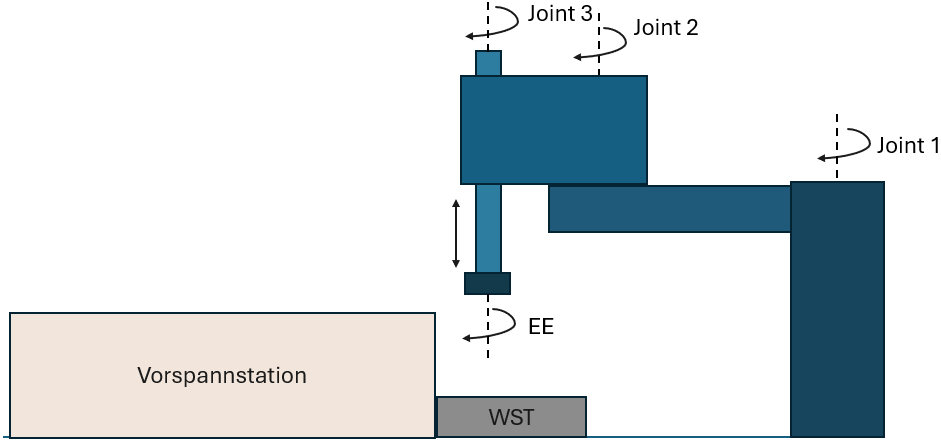
\includegraphics[width=0.8\linewidth]{Bilder/04_Konzeptentwicklung/Konzept_C.png}
    \caption{Zeichnung der Konzept C}
    \label{fig:concept_c}
\end{figure}

\textbf{Besonderheiten:}
\begin{itemize}
    \item Einsatz eines SCARA- bzw. SCARA-artigen Roboters als zentrale Kinematik
    \item Der Endeffektor greift einzelne Werkzeuge
    \item Die Bearbeitung erfolgt durch das jeweils aufgenommene Modul; danach wird es wieder zurückgelegt
    \item Der Roboter übernimmt damit sowohl die Handhabung (Greifen/Positionieren) als auch die Prozessausführung (Schrauben, Einpressen, Verschieben)
    \item Prozessmodule sind als wechselbare Einheiten ausgeführt (modulares Werkzeugkonzept)
\end{itemize}

\textbf{Vorteile:}
\begin{itemize}
    \item Hohe Flexibilität: unterschiedliche Prozessschritte können über verschiedene Module abgedeckt werden
    \item Geringer Bauraumbedarf im Vergleich zu Portal/Gantry, da keine große Brückenstruktur nötig ist
    \item Modular erweiterbar: neue Prozessmodule können ergänzt werden, ohne die gesamte Mechanik zu ändern
    \item Gute Eignung für Variantenfähigkeit (SLC / SLC-W) durch wechselbare Werkzeuge
\end{itemize}

\textbf{Nachteile:}
\begin{itemize}
    \item Höherer Steuerungs- und Integrationsaufwand
    \item Reproduzierbarkeit kritisch, weil Werkzeugaufnahme und Rückgabe Toleranzen einbringen
    \item Genauigkeit/Stabilität unter Prozesskräften kann schlechter sein als bei kartesischen Achsen
    \item Zusätzliche Risiken durch Kollisionen und komplexere Sicherheitsbetrachtungen
\end{itemize}

\subsection{Konzeptbewertung}
\subsubsection{Bewertungskriterien}
\label{sec:Bewertungskriterien}
Zur vergleichenden Bewertung der entwickelten Konzeptvarianten wurden geeignete Bewertungskriterien festgelegt, die sowohl technische als auch wirtschaftliche und organisatorische Aspekte des Systems abdecken. Ziel ist es, eine nachvollziehbare und möglichst objektive Entscheidungsgrundlage für die Auswahl eines Vorzugskonzepts zu schaffen.\cite{MKon_VL, ZangemeisterNutzwertanalyse}

Die Gewichtung der Bewertungskriterien erfolgte mithilfe eines Paarvergleichs. Dabei wurden die einzelnen Kriterien jeweils paarweise gegenübergestellt und hinsichtlich ihrer relativen Bedeutung für die Zielsetzung des Systems bewertet. Dieses Vorgehen ermöglicht es, subjektive Einzelmeinungen zu reduzieren und die Wichtigkeit der Kriterien systematisch und transparent abzuleiten.\cite{MKon_VL, ZangemeisterNutzwertanalyse}

Für den Paarvergleich wurde ein dreistufiges Bewertungsschema verwendet. Ein Wert von 2 bedeutet, dass ein Kriterium gegenüber dem Vergleichskriterium deutlich wichtiger ist. Ein Wert von 1 kennzeichnet eine gleichwertige Bedeutung beider Kriterien. Ein Wert von 0 wird vergeben, wenn das betrachtete Kriterium weniger wichtig ist als das gegenübergestellte.

Als Bewertungskriterien wurden folgende Aspekte definiert: Funktionalität, Robustheit, Montierbarkeit, Präzision, Kosten, Automatisierungsgrad, Effizienz und Zeit sowie Ästhetik. Diese Kriterien spiegeln die wesentlichen Anforderungen an die Montagestation wider und berücksichtigen sowohl den technischen Nutzen als auch praktische Gesichtspunkte der Umsetzung.

Aus der Summierung der Bewertungen ergibt sich für jedes Kriterium eine Zeilensumme, aus der anschließend die prozentuale Gewichtung berechnet wurde. Die prozentualen Anteile geben die relative Bedeutung der einzelnen Kriterien innerhalb der Nutzwertanalyse wieder. Zusätzlich wurde auf Basis dieser Gewichtung eine Rangfolge der Kriterien erstellt.

Die Ergebnisse des Paarvergleichs zeigen, dass insbesondere die Kriterien Funktionalität und Präzision eine hohe Bedeutung für die Bewertung der Konzepte besitzen. Ebenfalls relevant sind der Automatisierungsgrad sowie Aspekte der Effizienz und Prozesszeit. Kriterien wie Montierbarkeit, Kosten und Ästhetik wurden zwar berücksichtigt, weisen jedoch im Vergleich eine geringere Gewichtung auf.

Die so ermittelten Gewichtungsfaktoren bilden die Grundlage für die nachfolgende Nutzwertanalyse und fließen direkt in die Bewertung der einzelnen Konzeptvarianten ein.

{
\begin{table}[H]
\centering
\small
\setlength{\tabcolsep}{4pt}
\renewcommand{\arraystretch}{1.2}

\begin{tabular}{|l|c|c|c|c|c|c|c|c|c|c|c|}
\hline
 & \rotatebox{90}{Funktionalität} & \rotatebox{90}{Robustheit} & \rotatebox{90}{Montierbarkeit} &
 \rotatebox{90}{Präzision} & \rotatebox{90}{Kosten} & \rotatebox{90}{Automatisierungsgrad} &
 \rotatebox{90}{Effizienz und Zeit} & \rotatebox{90}{Ästhetik} &
 \rotatebox{90}{Zeilensumme} & \rotatebox{90}{\%} & \rotatebox{90}{Rang} \\
\hline
Funktionalität        & \textbf{X} & 2 & 2 & 1 & 2 & 2 & 2 & 2 & 13 & 23,21 & 1 \\
\hline
Robustheit            & 0 & \textbf{X} & 2 & 0 & 2 & 0 & 1 & 2 & 7  & 12,50 & 4 \\
\hline
Montierbarkeit        & 0 & 0 & \textbf{X} & 0 & 2 & 0 & 0 & 1 & 3  & 5,36  & 6 \\
\hline
Präzision             & 1 & 2 & 2 & \textbf{X} & 2 & 1 & 2 & 1 & 11 & 19,64 & 2 \\
\hline
Kosten                & 0 & 0 & 0 & 0 & \textbf{X} & 1 & 1 & 2 & 4  & 7,14  & 5 \\
\hline
Automatisierungsgrad  & 0 & 2 & 2 & 1 & 1 & \textbf{X} & 1 & 2 & 9  & 16,07 & 3 \\
\hline
Effizienz und Zeit    & 0 & 1 & 2 & 0 & 1 & 1 & \textbf{X} & 2 & 7  & 12,50 & 4 \\
\hline
Ästhetik              & 0 & 0 & 1 & 1 & 0 & 0 & 0 & \textbf{X} & 2  & 3,57  & 7 \\
\hline
\textbf{SUMME} & \textbf{X} & \textbf{X} & \textbf{X} & \textbf{X} & \textbf{X} & \textbf{X} & \textbf{X} & \textbf{X} & \textbf{56} & \textbf{100,00} & X \\
\hline
\end{tabular}

\caption{Paarvergleich zur Gewichtung der Bewertungskriterien für die Nutzwertanalyse}
\label{tab:bewertungskriterien_paarvergleich}
\end{table}
}

\subsubsection{Durchführung der Nutzwertanalyse}
Zur vergleichenden Bewertung der entwickelten Konzeptvarianten wurde eine Nutzwertanalyse durchgeführt. Grundlage hierfür bilden die in Abschnitt~\ref{sec:Bewertungskriterien} definierten und gewichteten Bewertungskriterien. Ziel der Nutzwertanalyse ist es, die unterschiedlichen Konzepte anhand einheitlicher Maßstäbe quantitativ miteinander zu vergleichen und so eine fundierte Entscheidungsbasis für die Auswahl eines Vorzugskonzepts zu schaffen.

Jede Konzeptvariante wurde für jedes Bewertungskriterium mit einer Punktzahl auf einer Skala von 1 bis 5 bewertet. Dabei steht der Wert 1 für eine sehr geringe Erfüllung des jeweiligen Kriteriums, während der Wert 5 eine sehr gute Erfüllung beschreibt. Die Bewertung erfolgte auf Basis der zuvor beschriebenen konzeptionellen Ausprägungen der Varianten sowie unter Berücksichtigung der technischen Machbarkeit, Systemkomplexität und des zu erwartenden Aufwands.

Zur Berechnung des Nutzwerts wurde die jeweilige Bewertung mit dem Gewichtungsfaktor des entsprechenden Kriteriums multipliziert. Auf diese Weise ergibt sich für jedes Kriterium ein gewichteter Teilwert. Die Summe aller gewichteten Teilwerte bildet den Gesamtnutzwert der jeweiligen Konzeptvariante.

Durch dieses Vorgehen wird sichergestellt, dass Kriterien von hoher Bedeutung, wie Funktionalität oder Präzision, stärker in das Gesamtergebnis einfließen als weniger gewichtete Kriterien. Gleichzeitig erlaubt die Nutzwertanalyse einen transparenten Vergleich der Konzepte, da sowohl Einzelbewertungen als auch deren Gewichtung nachvollziehbar dargestellt sind.

Die Ergebnisse der Nutzwertanalyse sind in Tabelle~\ref{tab:nutzwertanalyse} zusammengefasst.

{
\begin{table}[H]
\centering
\small
\setlength{\tabcolsep}{4pt}
\renewcommand{\arraystretch}{1.2}

\begin{tabular}{|l|c|c|c|c|c|c|c|}
\hline
\multirow{2}{*}{\textbf{Kriterium}} &
\multirow{2}{*}{\textbf{Faktor (\%)}} &
\multicolumn{2}{c|}{\textbf{Konzept 1}} &
\multicolumn{2}{c|}{\textbf{Konzept 2}} &
\multicolumn{2}{c|}{\textbf{Konzept 3}} \\
\cline{3-8}
 &  & \textbf{Bew.} & \textbf{Wert} & \textbf{Bew.} & \textbf{Wert} & \textbf{Bew.} & \textbf{Wert} \\
\hline
Funktionalität       & 23,21 & 5 & 116,07 & 5 & 116,07 & 4 & 92,86 \\
\hline
Robustheit           & 12,50 & 5 & 62,50  & 5 & 62,50  & 4 & 50,00 \\
\hline
Montierbarkeit       & 5,36  & 5 & 26,79  & 4 & 21,43  & 5 & 26,79 \\
\hline
Präzision            & 19,64 & 4 & 78,57  & 5 & 98,21  & 2 & 39,29 \\
\hline
Kosten               & 7,14  & 5 & 35,71  & 1 & 7,14   & 3 & 21,43 \\
\hline
Automatisierungsgrad & 16,07 & 3 & 48,21  & 3 & 48,21  & 3 & 48,21 \\
\hline
Effizienz und Zeit   & 12,50 & 5 & 62,50  & 4 & 50,00  & 1 & 12,50 \\
\hline
Ästhetik             & 3,57  & 3 & 10,71  & 4 & 14,29  & 3 & 10,71 \\
\hline
\textbf{SUMME} & \textbf{100,00} &  & \textbf{441,07} &  & \textbf{417,86} &  & \textbf{301,79} \\
\hline
\end{tabular}

\caption{Nutzwertanalyse der Konzeptvarianten}
\label{tab:nutzwertanalyse}
\end{table}
}

\subsubsection{Auswahl des Vorzugskonzepts}
Auf der Grundlage der durchgeführten Nutzwertanalyse lassen sich die Konzeptvarianten eindeutig miteinander vergleichen.

Das hohe Ergebnis von Konzept A ist insbesondere auf die sehr guten Bewertungen in den hoch gewichteten Kriterien Funktionalität, Präzision sowie Effizienz und Zeit zurückzuführen. Zudem weist diese Variante eine gute Kostenbewertung auf, was sich positiv auf den Gesamtnutzwert auswirkt. Insgesamt zeigt sich ein ausgewogenes Verhältnis zwischen technischer Leistungsfähigkeit und Systemaufwand.

Konzept B erzielt gute Ergebnisse in den Bereichen Präzision und Funktionalität, weist jedoch deutliche Nachteile bei den Kosten auf. Der hohe Investitionsaufwand, insbesondere durch den Einsatz einer hochintegrierten industriellen Montageanlage, wirkt sich trotz technischer Vorteile negativ auf das Gesamtergebnis aus.

Konzept C erreicht ebenfalls hohe Bewertungen in einzelnen technischen Kriterien, insbesondere in der Präzision. Allerdings führen der erhöhte Automatisierungs- und Integrationsaufwand sowie geringere Bewertungen in den Bereichen Effizienz und Kosten zu einem vergleichsweise niedrigen Gesamtnutzwert.

Aufgrund des höchsten Gesamtnutzwerts und des ausgewogenen Verhältnisses zwischen Nutzen, Aufwand und Umsetzbarkeit wird Konzept A als Vorzugskonzept ausgewählt und im weiteren Verlauf der Arbeit detailliert ausgearbeitet.
\clearpage
\section{Konzeptumsetzung}
\subsection{Mechanische Auslegung}
\subsubsection{Grundaufbau und Bauraum}
Der mechanische Aufbau des Montagesystems erfolgt auf einem ITEM-Arbeitstisch, der als stabile und standardisierte Basis dient. Dieser Tisch wurde nicht im Rahmen dieser Arbeit konstruiert, sondern als bestehende Infrastruktur genutzt. Die verfügbare Grundfläche beträgt 1200 × 760 mm und ermöglicht die Integration aller benötigten Baugruppen innerhalb der vorgegebenen Platzverhältnisse der Umgebung. Es gibt keine maßgebliche Begrenzung der Bauhöhe, sodass die vertikale Struktur des Systems frei gestaltet werden konnte.

Der Grundrahmen sowie die tragenden Strukturelemente des Systems bestehen aus ITEM-Profilen aus Aluminium-Strangpressmaterial. Diese Bauweise ermöglicht einen modularen und flexibel anpassbaren Aufbau, erleichtert spätere Erweiterungen oder Umbauten und entspricht gängigen industriellen Standards im Sondermaschinenbau.

Dieses System ist für eine einseitige Bedienung ausgelegt. Sämtliche Bedien- und Eingriffspunkte befinden sich auf der Vorderseite, während die Rückseite für technische Komponenten wie Antriebe, Pneumatik und elektrische Versorgung vorgesehen ist. Diese räumliche Trennung erleichtert sowohl die Bedienung im Produktionsbetrieb als auch Wartungs- und Servicearbeiten.

Der Gesamtaufbau ist in Abbildung~\ref{fig:gesamtaufbau_cad} dargestellt. Die Abbildung zeigt die Anordnung der einzelnen Module auf dem Arbeitstisch sowie deren räumliche Zuordnung zueinander. Das vollständige CAD-Modell des Gesamtaufbaus ist im Anhang~\ref{anhang:gesamtbau} abgelegt. Die zugehörigen Stücklisten sind den jeweiligen Teilsystemen zugeordnet und ebenfalls im Anhang dokumentiert.

\begin{figure}[H]
    \centering
    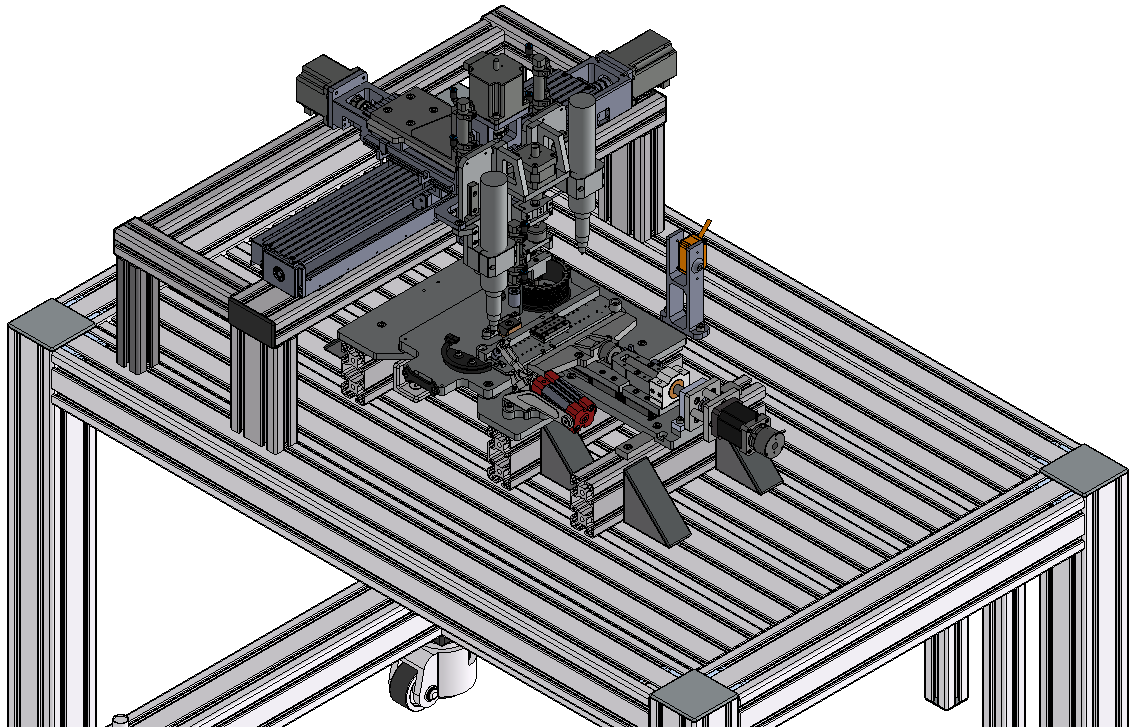
\includegraphics[width=0.95\linewidth]{Bilder/05_Konzeptumsetzung/Gesamtaufbau_CAD.png}
    \caption{Gesamtaufbau}
    \label{fig:gesamtaufbau_cad}
\end{figure}

\subsubsection{Modularer Aufbau der Teilsysteme}
Der mechanische Aufbau der Station ist modular gestaltet. Die einzelnen Funktionsbereiche sind in klar voneinander getrennte Teilsysteme untergliedert, bestehend aus der Werkstückaufnahme, der Vorspannstation, dem End-Effektor sowie dem Schraubmodul.

Diese Struktur zeichnet sich durch einen hohen Grad an Flexibilität aus. Einzelne Teilsysteme können bei Bedarf angepasst, ausgetauscht oder erweitert werden, ohne dass grundlegende Änderungen am Gesamtaufbau erforderlich sind. Zudem vereinfacht die modulare Auslegung sowohl den Aufbau der Station als auch deren spätere Wartung und Weiterentwicklung.

\subsubsection{Werkstückschnittstelle und Aufnahme}
Die Werkstückschnittstelle stellt die mechanische Verbindung zwischen dem Montagesystem und dem bestückten Werkstückträger (WST) dar. Sie ist als eigenständige Baugruppe ausgeführt und bildet die Grundlage für eine reproduzierbare Positionierung des Werkstücks während des gesamten Montageprozesses. Der Aufbau der Werkstückaufnahme erfolgt auf einer Basisplatte, die auf dem ITEM-Arbeitstisch montiert ist.

Zur Verbesserung der Zugänglichkeit wurde die Werkstückaufnahme um 80 mm gegenüber der Tischoberfläche erhöht. Diese Höhenanpassung ermöglicht eine erleichterte manuelle Platzierung und Entnahme des Werkstückträgers und verbessert die Greifbarkeit des WST im Produktionsbetrieb. Die Erhöhung wird durch den Einsatz von ITEM-Profilen realisiert, die als Distanzstruktur zwischen Arbeitstisch und Basisplatte dienen.

Die Positionierung des Werkstückträgers auf der Basisplatte erfolgt über zwei eingepresste Aufnahmebolzen. Dabei wird ein Rundbolzen sowie ein abgeflachter Bolzen verwendet. Diese Kombination gewährleistet eine eindeutige und wiederholgenaue Positionierung des WST in der Ebene, ohne eine Überbestimmung der Lagerung zu erzeugen. Durch die formschlüssige Führung über die Aufnahmebolzen ist sichergestellt, dass der Werkstückträger bei jedem Einlegen in derselben Lage und Orientierung positioniert wird.

Zur Fixierung des Werkstückträgers in vertikaler Richtung kommen zwei Spannvorrichtungen zum Einsatz, die den WST von oben gegen die Basisplatte pressen. Die Spannvorrichtungen sind so angeordnet, dass eine gleichmäßige Haltekraft auf den Werkstückträger wirkt und dieser während der nachfolgenden Prozessschritte sicher fixiert ist. Die Betätigung der Spannvorrichtungen erfolgt pneumatisch über ein Magnetventil, wodurch ein schnelles und zuverlässiges Spannen und Lösen des Werkstückträgers ermöglicht wird.

Der Bestückungsprozess beginnt mit dem manuellen Auflegen des bestückten Werkstückträgers auf die Basisplatte. Nach dem Aufsetzen auf die beiden Aufnahmebolzen wird der WST automatisch durch die Spannvorrichtungen fixiert. In diesem Zustand ist der Werkstückträger eindeutig positioniert und mechanisch gesichert, sodass die nachfolgenden Schritte des Vorspann- und Schraubprozesses unter reproduzierbaren geometrischen Bedingungen durchgeführt werden können.

Die Entnahme des Werkstückträgers erfolgt in umgekehrter Reihenfolge. Zunächst werden die Spannvorrichtungen gelöst, wodurch die Fixierung in vertikaler Richtung aufgehoben wird. Anschließend kann der Werkstückträger manuell von der Basisplatte abgehoben und aus der Station entnommen werden.

Der Gesamtaufbau der Werkstückaufnahme und die Basisplatte der Werkstückaufnahme mit den Positionier- und Spannelementen sind in Abbildung~\ref{fig:slc_vorspannen} dargestellt. Die detaillierte konstruktive Ausführung der Werkstückaufnahme ist in einer 2D-Zusammenbauzeichnung einschließlich der zugehörigen Stückliste im Anhang~\ref{anhang:Werkst.} dokumentiert.

\begin{figure}[htbp]
    \centering
    \begin{subfigure}[t]{0.48\linewidth}
        \centering
        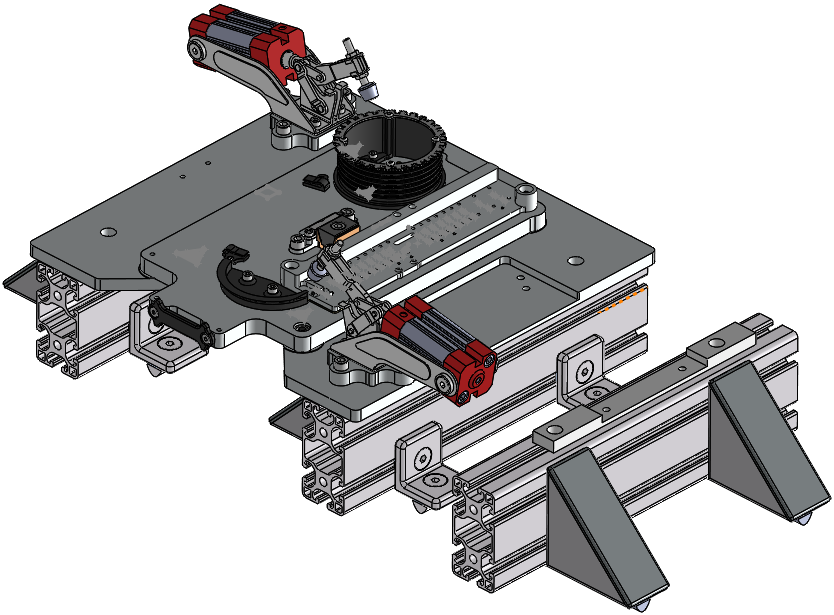
\includegraphics[width=\linewidth]{Bilder/05_Konzeptumsetzung/Werkstückaufnahme_gesamtbild.png}
        \caption{Werkstückaufnahme Gesamtbau}
        \label{fig:Werkstückaufnahme_gesamtbild_cad}
    \end{subfigure}
    \hfill
    \begin{subfigure}[t]{0.48\linewidth}
        \centering
        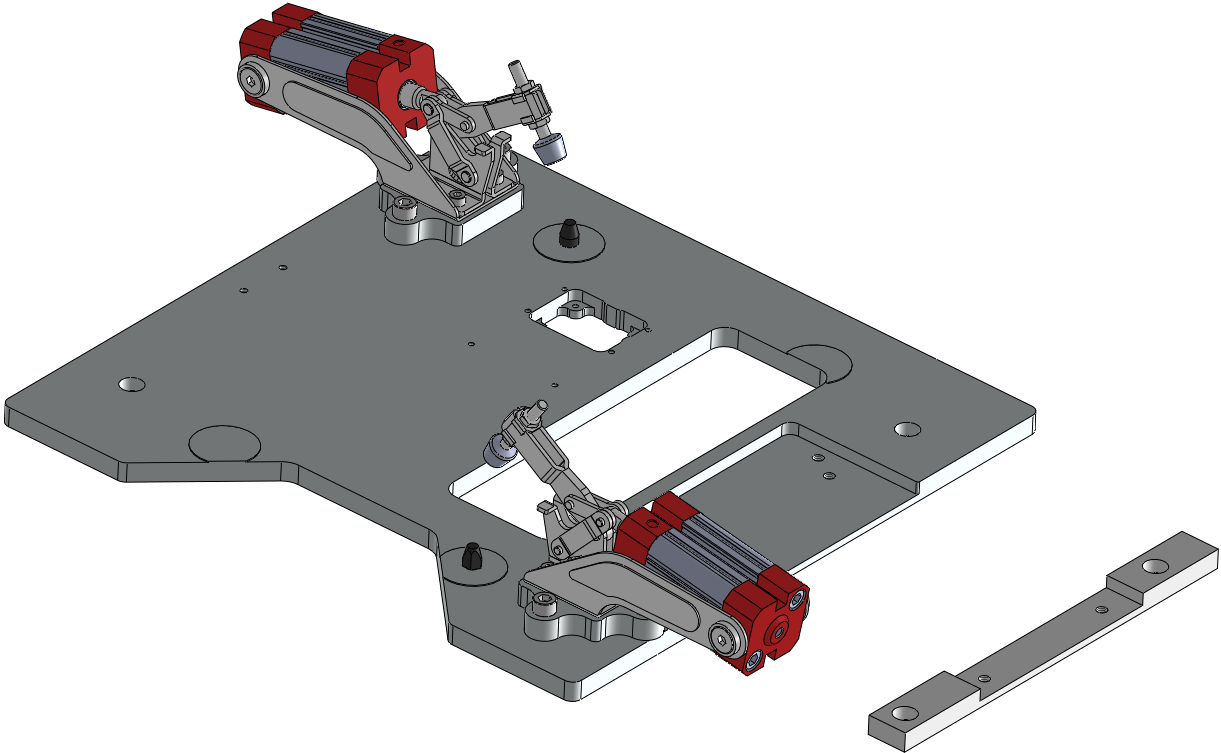
\includegraphics[width=\linewidth]{Bilder/05_Konzeptumsetzung/Werkstückaufnahme_bolzen.png}
        \caption{Basisplatte mit Positionier- und Spannelemente}
        \label{fig:Basisplatte mit Positionier- und Spannelemente}
    \end{subfigure}
    \caption{Darstellung der Werkstückaufnahme}
    \label{fig:slc_vorspannen}
\end{figure}

\subsubsection{End-Effektor (Werkzeugträger)}
Der End-Effektor bildet die zentrale mechanische Baugruppe zur Durchführung der Montageoperationen. Er ist als Werkzeugträger ausgeführt und vereint mehrere für den Aufbau der Linearführung erforderliche Funktionen innerhalb einer gemeinsamen, steifen Struktur. In den End-Effektor sind neben den beiden Schraubereinheiten sowohl das Keileinpresssystem als auch der Schlitten-Schieber integriert.

Die mechanische Grundstruktur des End-Effektors besteht aus einer tragenden Grundplatte, an der sämtliche Werkzeuge definiert positioniert und befestigt sind. Der End-Effektor ist mechanisch mit der Z-Achse der Station gekoppelt, sodass alle integrierten Werkzeuge gemeinsam verfahren werden. Dadurch bleibt die relative Lage der einzelnen Werkzeuge zueinander konstant.

Die beiden Schraubereinheiten sind symmetrisch angeordnet und ermöglichen das kontrollierte Verschrauben der Linearführung. Zur Vermeidung von Kollisionen während der Verfahrbewegungen der Gesamtstation sind beide Schrauber jeweils über pneumatische Kolbenstangenzylinder angebunden. Dadurch können die Schraubereinheiten bei Bedarf gezielt aus dem Arbeitsbereich zurückgezogen werden, bevor übergeordnete Achsbewegungen ausgeführt werden. Diese konstruktive Maßnahme erhöht die Betriebssicherheit und verhindert mechanische Kollisionen zwischen Werkzeug, Werkstück und End-Effektor.

Zentral im End-Effektor ist das Keileinpresssystem angeordnet, das mechanisch in die Grundstruktur eingebunden ist. Die zentrale Anordnung ermöglicht einen symmetrischen Kraftfluss während des Einpressvorgangs und reduziert unerwünschte Kippmomente. Das Keileinpresssystem ist zusätzlich mit zwei Gabellichtschranken ausgestattet, die als Endlagensensoren dienen und die Endpositionen des Einpressvorgangs überwachen.

Zusätzlich ist ein Schlitten-Schieber in den End-Effektor integriert, der zur definierten Positionierung einzelner Bauteile während des Montageablaufs dient. Auch dieser Schieber wird pneumatisch betätigt und ist mechanisch geführt, sodass der entsprechende Arbeitsschritt innerhalb desselben Koordinatensystems wie die übrigen Montageoperationen ausgeführt wird.

Alle drei im End-Effektor eingesetzten Rundzylinder – die beiden Zylinder für die Schraubereinheiten sowie der Zylinder für den Schlitten-Schieber – sind mit Endlagensensoren in Form von Näherungssensoren ausgestattet. Diese dienen der Überwachung der jeweiligen Endpositionen und können sicher stellen, dass übergeordnete Bewegungen der Station nur dann freigegeben werden, wenn sich alle Werkzeuge in einer kollisionsfreien Position befinden.

Bei der Auslegung des End-Effektors wurde besonderer Wert auf eine hohe Steifigkeit gelegt. Während des Schraub- und Einpressvorgangs wirken sowohl axiale als auch laterale Kräfte auf die Struktur. Relativbewegungen zwischen End-Effektor, Werkzeugen und Werkstück müssen daher möglichst gering gehalten werden, da sie sich unmittelbar auf die Montagequalität auswirken können. Die kompakte Bauweise sowie kurze Kraftflussketten tragen dazu bei, Verformungen zu minimieren und eine hohe Wiederholgenauigkeit zu gewährleisten.

Abbildung~\ref{fig:EE_iso} zeigt den End-Effektor in isometrischer Darstellung mit integrierten Schraubereinheiten, Keileinpresssystem und Schlitten-Schieber. In dieser Ansicht ist insbesondere die Anbindung der Schraubereinheiten an die pneumatischen Rundzylinder erkennbar.

Die detaillierte konstruktive Ausführung des End-Effektors ist in einer 2D-Zusammenbau\-zeichnung einschließlich der zugehörigen Teil-Stückliste im Anhang~\ref{anhang:ee_2d} dokumentiert. Die Ansteuerung der pneumatischen Zylinder sowie die Auswertung der Endlagensensoren werden in den Abschnitten zur \enquote{Aktorik und Antriebstechnik} (vgl. Abschnitt~\ref{sec:aktorik_antrieb}) sowie zur \enquote{Sensorik und Messtechnik} (vgl. Abschnitt~\ref{sec:sensorik_messtechnik}) behandelt.

\begin{figure}[H]
    \centering
    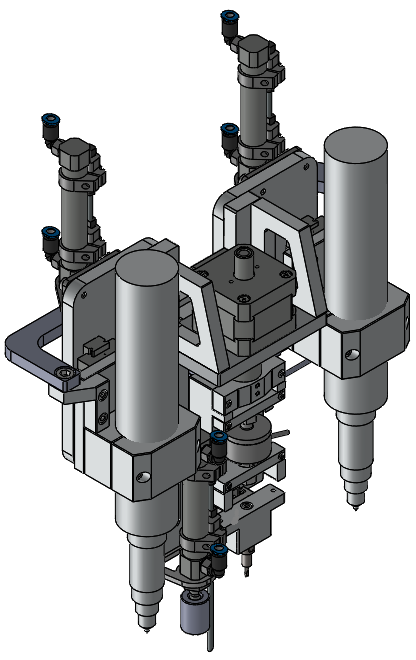
\includegraphics[width=0.40\linewidth]{Bilder/05_Konzeptumsetzung/End effektor iso anschicht.png}
    \caption{Isometrische Ansicht des End Effektors}
    \label{fig:EE_iso}
\end{figure}

\subsubsection{Achssystem}
Das Achssystem übernimmt die Positionierung des End-Effektors relativ zur Werkstückaufnahme und bildet die Grundlage für alle translatorischen Bewegungen innerhalb des Montagesystems. Es ist als kartesisches System ausgeführt und auf einem ITEM-Gestell montiert, das die notwendige Steifigkeit und Zugänglichkeit für den Montageprozess bereitstellt.

Als Linearachsen kommen GKS-Achsen der Firma GMT Europe zum Einsatz. Die Achsen sind modular aufgebaut und über Adapterplatten miteinander verbunden. Diese Adapterplatten dienen als definierte mechanische Schnittstellen zwischen den einzelnen Achsen sowie zwischen Achssystem und End-Effektor. Durch die Verwendung von Adapterplatten wird eine präzise Ausrichtung der Achsen zueinander gewährleistet und der mechanische Integrationsaufwand reduziert.

Das Achssystem ist vollständig auf dem ITEM-Gestell aufgebaut, wie in Abbildung~\ref{fig:roboter} dargestellt. Das Gestell übernimmt dabei sowohl die Funktion der tragenden Struktur als auch die Einbindung des Achssystems in den Gesamtaufbau der Station. Die offene Bauweise des ITEM-Gestells erleichtert zudem den Zugang für Montage-, Wartungs- und Servicearbeiten.

Alle eingesetzten Achsen sind mit Endlagensensoren ausgestattet. Pro Achse kommen jeweils zwei Gabellichtschranken zum Einsatz, die die Endpositionen der Verfahrbewegung absichern. Dadurch wird sichergestellt, dass die Bewegungen der Achsen ausschließlich innerhalb definierter mechanischer Grenzen erfolgen. Die Endlagensensoren dienen sowohl der Referenzierung als auch zum Schützen des Achssystems.

Die mechanische Auslegung des Achssystems ist auf eine hohe Wiederholgenauigkeit ausgelegt. Die Führung der Achsen sowie deren Anbindung über Adapterplatten sorgen für eine stabile Kraftübertragung und minimieren Relativbewegungen zwischen den einzelnen Baugruppen. Damit bildet das Achssystem die Grundlage für die präzise Positionierung des End-Effektors während des Vorspann-, Einpress- und Schraubprozesses.

Die detaillierte konstruktive Ausführung des Achssystems ist in einer 2D-Zusammenbau\-zeichnung einschließlich der zugehörigen Teil-Stückliste im Anhang~\ref{anhang:achssystem} dokumentiert.

Die Ansteuerung der Achsen sowie die Auswertung der Endlagensensoren werden in den Abschnitten zur \enquote{Aktorik und Antriebstechnik} (vgl. Abschnitt~\ref{sec:aktorik_antrieb}) sowie zur \enquote{Sensorik und Messtechnik} (vgl. Abschnitt~\ref{sec:sensorik_messtechnik}) behandelt.

\begin{figure}[H]
    \centering
    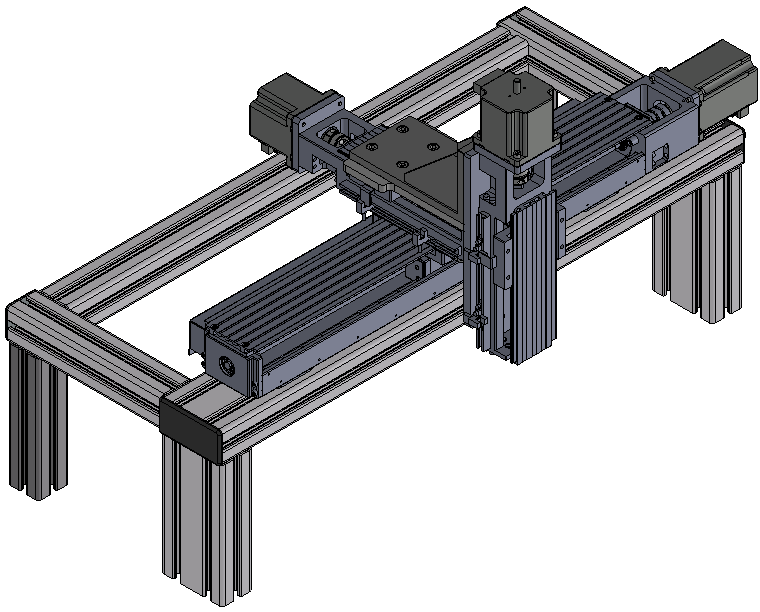
\includegraphics[width=0.45\linewidth]{Bilder/05_Konzeptumsetzung/Achssystem.png}
    \caption{Achssystem}
    \label{fig:roboter}
\end{figure}

\subsection{Aktorik und Antriebstechnik}
\label{sec:aktorik_antrieb}
\subsubsection{Eingesetzte Aktoren}
In diesem Abschnitt werden die im Montagesystem eingesetzten Aktoren beschrieben, deren Auswahl und Integration Bestandteil dieser Arbeit sind. Der Fokus liegt dabei auf den Linearachsen mit zugehörigen Motoren, den Schraubereinheiten sowie den pneumatischen Aktoren für Bewegungs- und Spannfunktionen.

Die Antriebe des Vorspannsystems sowie des Keileinpresssystems wurden nicht neu ausgelegt. Diese Systeme waren bereits als funktionsfähige und erprobte Lösungen vorhanden und wurden als Stand der Technik übernommen. Sie werden daher in diesem Kapitel nicht ausgelegt.

Für die Positionieraufgaben im System werden drei Linearachsen eingesetzt. Die Auswahl der Achsen sowie der zugehörigen Schrittmotoren erfolgte im Rahmen dieser Arbeit auf Basis der geforderten Verfahrwege, der zu bewegenden Massen sowie der erforderlichen Positioniergenauigkeit.

Als Schraubwerkzeuge kommen elektrische Schrauber des Herstellers Kolver zum Einsatz, die bereits im Unternehmen verfügbar sind. Diese wurden gezielt in das Montagekonzept integriert. Ergänzend dazu werden pneumatische Rundzylinder für einfache lineare Bewegungen sowie eine vorhandene Spannvorrichtung zur Fixierung der Bauteile eingesetzt.

Tabelle~\ref{tab:aktoren_uebersicht} fasst die Aktoren hinsichtlich Typ, Funktion und Einsatzbereich zusammen.\cite{ds_gmt_gka_gks,ds_nanotec_sca5618,ds_nanotec_scb6018,ds_kolver_mito15ca,ds_kolver_nato50ca,ds_kolver_edu2ae,ds_festo_dsnu,ds_gn860}

\begin{table}[H]
\centering
\small
\setlength{\tabcolsep}{4pt}
\renewcommand{\arraystretch}{1.2}
\begin{tabular}{|p{3.0cm}|p{4.8cm}|p{4.0cm}|p{2.8cm}|}
\hline
\textbf{Aktor} & \textbf{Typ / Bezeichnung} & \textbf{Funktion im System} & \textbf{Zuordnung} \\
\hline
Linearachse X & GKA4270-500-12N-P10 & Positionierung in X-Richtung & Positionierachse \\
\hline
Linearachse Y & GKS3060-50-12N-P5 & Positionierung in Y-Richtung & Positionierachse \\
\hline
Linearachse Z & GKS3060-50-12N-P5 & Positionierung in Z-Richtung & Positionierachse \\
\hline
Schrittmotor X & Nanotec SCA5618L4204-B2 & Antrieb der X-Achse & Elektrischer Antrieb \\
\hline
Schrittmotor Y/Z & Nanotec SCB6018M4204-B & Antrieb der Y- und Z-Achse & Elektrischer Antrieb \\
\hline
Schrauber SLC-24 & MITO15CA & Verschrauben von M2-Schrauben & Prozessaktor \\
\hline
Schrauber SLC-17 & NATO50CA/TA & Verschrauben von M1{,}4-Schrauben & Prozessaktor \\
\hline
Pneumatikzylinder & DSNU-S-12-40-P-MQ & Bewegung der Schraubereinheiten und des Schlitten-Schiebers & Hilfsaktor \\
\hline
Spannvorrichtung & GN 860-75-CP-M & Fixierung des Werkstückträgers während der Montage & Spanntechnik \\
\hline
\end{tabular}
\caption{Übersicht der eingesetzten Aktoren und deren funktionale Zuordnung}
\label{tab:aktoren_uebersicht}
\end{table}

\subsubsection{Achssysteme}
Die Achssysteme übernehmen im Montagesystem ausschließlich Positionieraufgaben. Für diesen Zweck wurden vorkonfigurierte Linearachsen ausgewählt, die von GMT Europe bezogen wurden. Alle Achsen arbeiten mit Kugelgewindetrieben und sind jeweils einem eigenen Schrittmotor zugeordnet.

Die X-Achse wird durch eine Linearachse des Typs GKA4270-500-12N-P10 realisiert. Sie besitzt einen effektiven Verfahrweg von 413\,mm und dient der horizontalen Positionierung der Funktionseinheiten. Aufgrund der vergleichsweise großen Verfahrstrecke wurde diese Achse mit einer Spindelsteigung von 10\,mm ausgeführt, um eine ausreichende Verfahrgeschwindigkeit bei gleichzeitig robuster Kraftübertragung zu gewährleisten. Die hohe dynamische und statische Tragfähigkeit der Achse stellt sicher, dass die im Betrieb auftretenden Lasten mit ausreichender Sicherheitsreserve innerhalb der zulässigen Grenzwerte liegen \cite{ds_gmt_gka_gks}.

Für die Y- und Z-Achse werden Linearachsen des Typs GKS3060-50-12N-P5 eingesetzt. Diese Achsen besitzen einen Verfahrweg von jeweils 50\,mm und sind für kurze, präzise Zustellbewegungen ausgelegt. Die geringere Spindelsteigung von 5\,mm ermöglicht eine höhere Auflösung und eine feinere Positionierung, was insbesondere für die Zustellbewegung der Schraubereinheiten relevant ist. Auch hier liegen die zulässigen Lasten der Achsen deutlich über den im Prozess auftretenden Belastungen \cite{ds_gmt_gka_gks}.

Als Antriebe kommen Schrittmotoren des Herstellers Nanotec zum Einsatz. Die X-Achse wird von einem Motor des Typs SCA5618L4204-B2 mit einem Haltemoment von 230\,Ncm angetrieben. Für die Y- und Z-Achse werden Motoren des Typs SCB6018M4204-B mit einem Haltemoment von 200\,Ncm verwendet. Alle Motoren besitzen einen Schrittwinkel von 1{,}8° und damit 200 Vollschritte pro Umdrehung \cite{ds_nanotec_sca5618,ds_nanotec_scb6018}.

Aus der Kombination von Schrittwinkel, eingestellter Microstepping-Auflösung und Spindelsteigung ergibt sich für alle drei Achsen eine theoretische lineare Auflösung von \qty{1,56}{\micro\meter} pro Microstep. Die eingesetzte Trinamic-Motorsteuerung unterstützt diese Microstepping-Betriebsart hardwareseitig. Ein Mikroschritt stellt dabei eine elektronisch geregelte Unterteilung eines Vollschrittes dar, wodurch eine feinere Positionsauflösung sowie ein ruhigerer Motorlauf erreicht werden. Dieser Wert liegt deutlich unterhalb der in der Anforderungsliste definierten Toleranz von \qty{15}{\micro\metre} und erfüllt damit die Anforderungen an die Positionierauflösung der Achssysteme. Rechnerisch wären hierfür bereits 4 Microsteps pro Vollschritt für die X-Achse sowie 2 Microsteps pro Vollschritt für die Y- und Z-Achse ausreichend. Die tatsächlich gewählten Einstellungen von 32 Microsteps für die X-Achse sowie 16 Microsteps für die Y- und Z-Achse stellen somit eine zusätzliche Reserve hinsichtlich Auflösung und Laufruhe dar. Die zugehörigen Berechnungen zur Schrittauflösung sind in Anhang~\ref{anhang:berechnungen} dargestellt.

Auf der Grundlage der durchgeführten Auslegungs- und Plausibilitätsberechnungen wurden für die Achsen maximale lineare Geschwindigkeiten von etwa \qty{23,8}{\mm\per\s} sowie maximale Beschleunigungen von rund \qty{182}{\mm\per\s\tothe{2}} festgelegt. Diese berechneten Sollwerte wurden anschließend durch eine geeignete Wahl der Steuerungsparameter umgesetzt. Daraus resultieren bei idealisierter Betrachtung reine Fahrzeiten von etwa \qty{17}{\second} für den vollen X-Verfahrweg sowie rund \qty{2}{\second} für einen 50-mm-Hub auf der Y- und Z-Achse. Die detaillierten Berechnungen zu Geschwindigkeit, Beschleunigung und Fahrzeit sind im Anhang~\ref{anhang:berechnungen} aufgeführt.

Zur Vermeidung von Schrittverlusten wurde die Motorauswahl zusätzlich über den erforderlichen Drehmomentbedarf überprüft. Aus den maximalen Achsgeschwindigkeiten ergeben sich Motordrehzahlen von etwa \qty{143}{\per\minute} für die X-Achse sowie \qty{286}{\per\minute} für die Y- und Z-Achse. Die Berechnung der notwendigen Antriebsmomente zeigt, dass diese deutlich unterhalb der bei diesen Drehzahlen verfügbaren Pull-out-Momente der eingesetzten Motoren liegen. Das Pull-out-Moment beschreibt dabei das maximal verfügbare Drehmoment eines Schrittmotors bei einer gegebenen Drehzahl, bei dem der Motor dem vorgegebenen Schrittsignal noch synchron folgen kann, ohne Schritte zu verlieren. Dabei wurde neben dem Haltemoment auch der Drehzahlbereich berücksichtigt, in dem die Achsen im Betrieb bewegt werden. Somit ist sichergestellt, dass die Motoren auch unter Last zuverlässig arbeiten und es nicht zu Schrittverlusten kommt. Der vollständige Drehmomentnachweis ist in Anhang~\ref{anhang:berechnungen} dokumentiert.

Die vollständigen Berechnungen zur Auflösung, Geschwindigkeit, Beschleunigung sowie zum Drehmomentnachweis sind zusammenfassend im Anhang~\ref{anhang:berechnungen} detailliert dokumentiert.


\subsubsection{Pneumatische Aktoren}
Pneumatische Aktoren werden im Montagesystem gezielt für unterstützende Bewegungen eingesetzt, bei denen keine hochgenaue Positionierung erforderlich ist. Ihr Einsatz dient insbesondere der Prozessentkopplung und der Reduktion zusätzlicher Bewegungen der elektrischen Achssysteme.

Für diese Aufgaben werden drei pneumatische Rundzylinder des Typs DSNU-S-12-40-P-MQ von Festo eingesetzt. Zwei dieser Zylinder sind den Schraubereinheiten zugeordnet. Sie sorgen dafür, dass die Schrauber beim Ansetzen der Schrauben definiert und mit ausreichender Kraft in Richtung des Schraubenkopfes zugestellt werden. Dadurch wird sichergestellt, dass der Schrauber korrekt im Schraubenkopf sitzt und ein unerwünschtes \enquote{Freidrehen} des Werkzeugs vermieden wird. Diese pneumatische Zustellbewegung unterstützt somit direkt die Prozesssicherheit des Schraubvorgangs.\cite{ds_festo_dsnu}

Der dritte pneumatische Zylinder wird für die Bewegung des Schlitten-Schiebers verwendet. Auf eine zusätzliche Bewegung des gesamten Endeffektors in Z-Richtung kann dadurch verzichtet werden, was den Bewegungsablauf vereinfacht und die mechanische Belastung der Achssysteme reduziert.

Die eingesetzten Rundzylinder besitzen einen Kolbendurchmesser von 12 mm und einen Hub von 40 mm. Bei einem Betriebsdruck von \qty{0,6}{\mega\pascal} ergibt sich eine theoretische Zylinderkraft von rund \qty{68}{\newton}, die für die beschriebenen Bewegungsaufgaben ausreichend ist.\cite{ds_festo_dsnu}

Zusätzlich wird eine vorhandene Spannvorrichtung des Typs GN 860-75-CP-M eingesetzt. Diese dient der Fixierung des Werkstückträgers während des Schraubprozesses und stellt sicher, dass die Bauteile während der Montage lagegenau gehalten werden. Die Spannvorrichtung wurde ohne konstruktive Änderungen in das System integriert.\cite{ds_gn860}

Durch den gezielten Einsatz pneumatischer Aktoren für diese unterstützenden Funktionen kann sich die elektrische Antriebstechnik auf präzise Positionieraufgaben konzentrieren. Dies trägt zu einem übersichtlichen Systemaufbau sowie zu einer robusten und prozesssicheren Umsetzung der Montageabläufe bei.

\subsubsection{Schraubeinheiten}
Die Schraubereinheiten stellen zentrale Prozessaktoren des Montagesystems dar und sind maßgeblich für die Montagequalität verantwortlich. Abhängig von der Baugröße des Positionierers kommen unterschiedliche Schraubermodelle zum Einsatz.

Für Positionierer der Baugröße SLC-24 mit M2-Schrauben wird ein Schrauber des Typs MITO15CA verwendet. Dieser deckt einen Drehmomentbereich von 0,35 Nm bis 1,5 Nm ab und arbeitet mit Drehzahlen zwischen 450 und 850 $\min^{-1}$. Für Positionierer der Baugröße SLC-17 mit M1,4-Schrauben kommt ein Schrauber des Typs NATO50CA/TA zum Einsatz, dessen Drehmomentbereich zwischen 0,05 Nm und 0,7 Nm liegt.\cite{ds_kolver_nato50ca, ds_kolver_mito15ca}

Die Schrauber werden über externe Controller der EDU2AE-Serie betrieben und über digitale Ein- und Ausgänge in die Anlagensteuerung eingebunden. Die Anzahl der Schrauben pro Montage variiert in Abhängigkeit von der Länge und Breite des jeweiligen Positionierers, was durch die flexible Prozessführung berücksichtigt wird.\cite{ds_kolver_edu2ae}

Die Schrauber sind mechanisch an die jeweiligen Z-Achsen angebunden. Die Zustellbewegung erfolgt ausschließlich entlang der Z-Achse.

\subsubsection{Zusammenfassung der Antriebsauslegung}
Die im Rahmen dieser Arbeit ausgewählte Aktorik deckt alle erforderlichen Bewegungs- und Montagefunktionen des Systems zuverlässig ab. Die Kombination aus elektrisch angetriebenen Linearachsen für präzise Positionieraufgaben und pneumatischen Aktoren für Hilfs- und Spannfunktionen hat sich als zweckmäßig und übersichtlich erwiesen.

Die Achssysteme und Motoren verfügen über ausreichende Leistungsreserven, sodass ein stabiler Betrieb auch bei variierenden Prozessbedingungen gewährleistet ist. Bestehende Antriebslösungen für das Vorspannsystem und das Keileinpresssystem wurden bewusst übernommen, um auf erprobte Konzepte zurückzugreifen und den Fokus der Arbeit auf die Auslegung der Positionier- und Schraubprozesse zu legen.

\subsection{Sensorik und Messtechnik}
\label{sec:sensorik_messtechnik}

\subsubsection{Ziel der Sensorik}
Die Sensorik dient der Überwachung von Positionen, Kräften und Zuständen innerhalb des Montageprozesses. Ziel ist es, eine sichere und reproduzierbare Durchführung der einzelnen Prozessschritte zu gewährleisten sowie fehlerhafte Zustände frühzeitig zu erkennen. Die Sensoren werden dabei primär zur Referenzierung, Prozessfreigabe und Plausibilitätsprüfung eingesetzt und tragen wesentlich zur Erhöhung der Prozesssicherheit bei.

\subsubsection{Positions- und Referenzsensoren}
Zur Referenzierung und Endlagenüberwachung der motorisierten Achsen sind an allen Linearachsen jeweils zwei Gabellichtschranken des Typs Panasonic PM-F25 eingesetzt. Der in Motornähe montierte Sensor dient zur Referenzfahrt und definiert den Nullpunkt der jeweiligen Achse. Der zweite Sensor übernimmt die Funktion der Endlagenüberwachung und verhindert unzulässige Verfahrbewegungen.\cite{ds_panasonic_pmf25}

Die Sensoren sind direkt an den Linearachsen montiert. Im Vorspannsystem waren ursprünglich keine Endlagensensoren vorgesehen; diese wurden im Rahmen dieser Arbeit ergänzend an der Adapterplatte nachgerüstet. Auch im Keileinpresssystem sind Endlagensensoren an der Adapterplatte angebracht, deren mechanische Integration bereits im Vorfeld erfolgte. Die Endlagensensoren sind als digitale Schaltsensoren ausgeführt und elektrisch angebunden.

An den eingesetzten Rundzylindern werden jeweils zwei Näherungssensoren zur Erfassung der Kolbenendlagen verwendet. Hier kommen Sensoren des Typs Festo SMT-8M-A-PS-24V-E-0,3-M8D zum Einsatz, die mithilfe von Festo SMBR 8-12 Haltern direkt am Zylinder montiert sind. Diese Sensoren ermöglichen eine zuverlässige Zustandsüberwachung der pneumatischen Bewegungen und dienen ebenfalls der Prozessfreigabe.\cite{ds_festo_smt8m, ds_festo_smbr}

\subsubsection{Kraftmesstechnik}
Zur Überwachung der aufgebrachten Kräfte sind in der Vorspannmechanik sowie im Keileinpresssystem Kraftmessdosen integriert. Die verwendeten Sensoren waren Bestandteil eines bestehenden Systems und wurden im Rahmen dieser Arbeit übernommen. Im Keileinpresssystem wird eine Kraftmessdose des Typs KM26z-50N eingesetzt, während in der Vorspannmechanik eine Kraftmessdose des Typs KM26z-500N verwendet wird.\cite{ds_km26z_50n, ds_km26z_500n}

Die Kraftmessdosen sind jeweils zwischen Aktor und mechanischer Struktur angeordnet, sodass die tatsächlich eingeleitete Kraft direkt erfasst werden kann. Die Sensorsignale werden analog ausgegeben und über externe Messverstärker des Typs ME-Meßsysteme GSV-1H 010/250/2 aufbereitet. Diese Verstärker wurden im Zuge dieser Arbeit ergänzt, da sie im ursprünglichen System nicht vorhanden waren. Die erfassten Kraftwerte dienen dem Vergleich von Soll- und Ist-Kraft und ermöglichen eine Überwachung der eingestellten Vorspannung während des Montageprozesses.\cite{ds_me_gsv1h}

\subsubsection{Optische Messtechnik}
Zur berührungslosen Erfassung der Schlittenposition wird ein Laser-Triangulationssensor des Typs Micro-Epsilon optoNCDT 1220 mit einem Messbereich von 500 mm eingesetzt. Der Sensor misst die Schlittenposition in X-Richtung und ermöglicht eine präzise Bestimmung der Lage während des Montageablaufs. Die Wiederholgenauigkeit beträgt \qty{50}{\micro\metre}. Die Linearitätsabweichung des Laser-Triangulationssensors liegt im zentralen Messbereich ($< \qty{750}{\micro\metre}$) unter \num{0,15}\,\% des Full-Scale-Outputs (FSO) und beträgt über den gesamten Messbereich bis \qty{1500}{\micro\metre} maximal \num{0,30}\,\% FSO.

Der Einsatz eines Laser-Triangulationssensors ist insbesondere aufgrund der sehr kleinen verfügbaren Messoberfläche erforderlich. Als Messziel dient der Schraubenkopf des Schlittens mit einem Durchmesser von etwa 4 mm, wodurch taktile Messverfahren nur eingeschränkt geeignet wären. Die Signalausgabe erfolgt analog über eine $4\text{--}20\text{ mA}$-Schnittstelle und wird von der Steuerung zur Positionsüberwachung und Plausibilitätsprüfung genutzt.\cite{ds_microepsilon_optoncdt1220}

\subsection{Steuerungskonzept}
\subsubsection{Grundidee der Steuerungsarchitektur}
Die Steuerungsarchitektur basiert auf einer funktionalen Trennung zwischen Bewegungssteuerung und übergeordneter Prozess- und Ablaufsteuerung. Die Ansteuerung der motorisierten Achsen erfolgt über einen Trinamic TMCM-6110 Motorkontroller, während die Einbindung der Peripherie sowie die Prozesslogik über ein modulares WAGO-I/O-System realisiert wird. Diese Aufteilung ermöglicht eine übersichtliche Struktur, reduziert die Komplexität der Einzelkomponenten und erleichtert eine spätere Erweiterung des Systems.

Der Einsatz des WAGO-Systems wurde erforderlich, da die am TMCM-6110 verfügbaren Ein- und Ausgänge für die vollständige Anbindung aller Aktoren und Sensoren nicht ausreichten. Durch die Kombination beider Systeme konnte eine klare Trennung zwischen Bewegungsfunktionen und prozessrelevanten Ein- und Ausgängen umgesetzt werden.

Zur übersichtlichen Darstellung der Ein- und Ausgänge sowie der angebundenen Aktoren und Sensoren ist in Abbildung~\ref{fig:sys_archi} ein Blockdiagramm dargestellt. Es zeigt die Zuordnung der Peripheriekomponenten zum TMCM-6110 sowie die Anbindung des Rechners und des WAGO-I/O-Systems. Die vollständigen elektrischen Schaltpläne sind im Anhang~\ref{anhang:schaltplan} abgelegt und dienen dort der detaillierten Nachvollziehbarkeit und Referenz.

\begin{figure}[H]
    \centering
    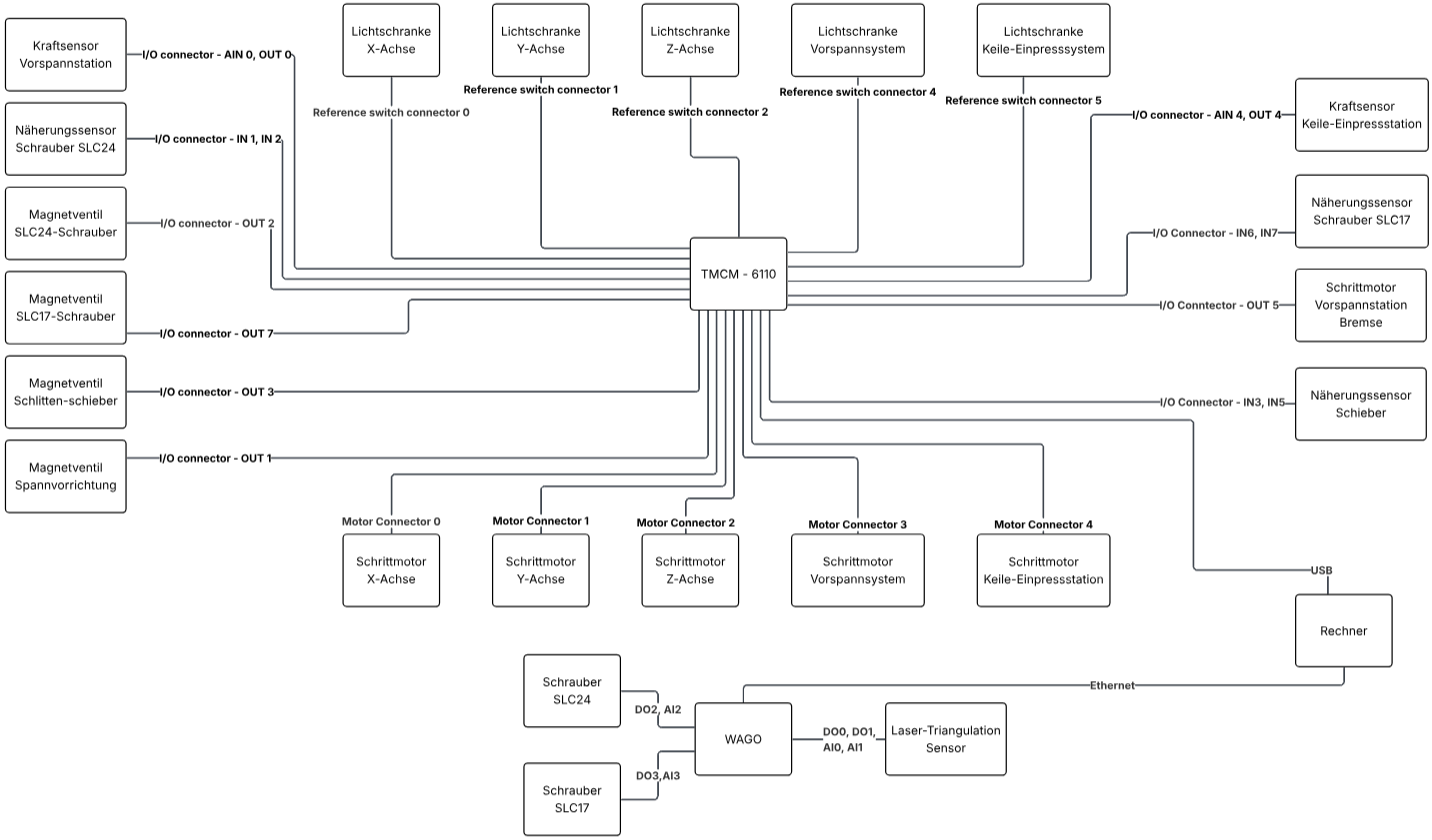
\includegraphics[width=1\linewidth]{Bilder/05_Konzeptumsetzung/Systemarchi.png}
    \caption{I/O-Belegung und Systemübersicht}
    \label{fig:sys_archi}
\end{figure}

\subsubsection{Einbindung der Aktoren}
Alle fünf eingesetzten Motoren sind direkt an die Motorkontroller-Ausgänge des TMCM-6110 angebunden. Die zugehörigen Endlagensensoren sind an den dafür vorgesehenen Referenz- und Endschalter-Eingängen des Motorkontrollers angeschlossen und dienen der Referenzfahrt sowie der Endlagenüberwachung.

Die Ansteuerung der pneumatischen und elektrischen Aktoren erfolgt über digitale Ausgänge. Dazu zählen eine Bremse für den Motor des Vorspannsystems, vier Magnetventile für die beiden Schraubereinheiten, den Schlittenschieber sowie die Spannvorrichtung. Zusätzlich sind zwei digitale Ausgänge zur Tara-Funktion der Kraftmessverstärker vorgesehen. Diese Ausgänge ermöglichen das gezielte Zurücksetzen der Kraftmesssignale vor Beginn eines Messvorgangs. Die Tara-Funktionen der Kraftmessverstärker sind ebenfalls über Relais angebunden. Hintergrund ist, dass die digitalen Ausgänge des TMCM-6110 als Open-Drain-Ausgänge ausgeführt sind, während die eingesetzten Kraftmessverstärker ein +24-V-Signal zur Auslösung der Tara-Funktion benötigen. Die Relais dienen hierbei zur galvanischen Trennung sowie zur Anpassung der Signalpegel zwischen dem Motorkontroller und dem Verstärkereingang.\cite{man_trinamic_tmcm6110}

\subsubsection{Einbindung der Sensoren}
Die Näherungssensoren der Rundzylinder sind als digitale Eingänge ausgeführt. Insgesamt sind sechs digitale Eingänge belegt, wobei pro Rundzylinder jeweils zwei Sensoren zur Erfassung der Endlagen eingesetzt werden.

Die Kraftmessdosen werden über analoge Eingänge angeschlossen. Die verstärkten Kraftsignale der beiden Messstellen werden an zwei analoge Eingänge des Systems geleitet und dienen der Überwachung der aufgebrachten Kräfte im Vorspann- und Keileinpressprozess.

Der Laser-Triangulationssensor ist ebenfalls über einen analogen Eingang angebunden und liefert sein Messsignal als $4\text{--}20\text{ mA}$-Stromsignal. Zusätzlich werden Status- und Fehlerinformationen des Lasers sowie Rückmeldesignale der Schrauber als digitale Signale erfasst.

\subsubsection{WAGO-I/O-System}
Das WAGO-I/O-System ist modular aufgebaut und besteht aus einem Modbus-Koppler des Typs WAGO 750-362, einer Potentialeinspeisung WAGO 750-602 sowie mehreren Ein- und Ausgangsmodulen. Zur Ansteuerung der Aktoren wird ein digitales Ausgangsmodul WAGO 750-531 eingesetzt. Die Erfassung der analogen Sensorsignale erfolgt über zwei analoge Eingangsmodule des Typs WAGO 750-466. Den Abschluss des Systems bildet ein Endmodul WAGO 750-600.\cite{ds_wago_750362, ds_wago_750602, ds_wago_750531, ds_wago_750466, ds_wago_750600}

An die digitalen Ausgänge des WAGO-Systems sind die Ein- und Ausschaltung des Lasers sowie dessen Funktionseingang jeweils über Relais angebunden. Darüber hinaus werden die Startsignale der beiden Schrauber (MITO15CA und NATO50CA/TA) über Relais geschaltet. Während das WAGO-Ausgangsmodul beim Aktivieren eines digitalen Ausgangs ein +24-V-Signal liefert, erwarten die angeschlossenen Geräte ein Open-Drain- bzw. potenzialfreies Schaltsignal. Die Relais übernehmen in diesem Fall die notwendige Signalumsetzung und stellen eine kompatible Anbindung der Komponenten sicher. Die analogen Eingänge erfassen das Stromsignal des Lasersensors. Status- und Rückmeldesignale der Schrauber sowie das Fehlerausgangssignal des Lasers werden als digitale Signale ausgewertet.

\subsection{Ablaufverfahren und zeitliche Auslegung des Prozesses}
Im Folgenden wird der konzeptionell vorgesehene Montageablauf des Systems beschrieben. 
Zusätzlich werden für die einzelnen Prozessschritte berechnete Zeitanteile angegeben, um die zeitliche Machbarkeit des Gesamtkonzepts zu bewerten.

\begin{longtable}{|c|p{7.5cm}|c|p{3.5cm}|}
\hline
\textbf{Nr.} & \textbf{Prozessschritt} & \textbf{Zeit [s]} & \textbf{Achsen / Aktoren} \\
\hline
\endfirsthead

\hline
\endhead
\endfoot
\endlastfoot

1 &
Synchrones Verfahren aller Achsen von Referenz- in Startposition (X mittig positioniert, Y auf hintere Führung ausgerichtet) &
6.0 &
X, Y, Z (überlagert) \\
\hline

2 &
Einleiten des Vorspannvorgangs &
3.5 &
Vorspannaktor \\
\hline

3 &
Positionierung der Z-Achse zur ersten Schraubposition &
1.0 &
Z \\
\hline

4 &
Verschraubung der ersten Schraube mit automatischem Schrauber (MITO); geringfügige Korrekturbewegungen zur exakten Ausrichtung &
2.0 &
Schrauber, X/Y (fein) \\
\hline

5 &
Aktivierung des Schiebers und Verschieben des Schlittens zur Vorbereitung der nächsten Schraubposition &
2.2 &
Schieberaktor \\
\hline

6 &
Positionierung zur zweiten Schraubposition durch geringe Korrekturbewegungen &
1.0 &
X, Y \\
\hline

7 &
Verschraubung der zweiten Schraube mit automatischem Schrauber &
2.0 &
Schrauber \\
\hline

8 &
Erneutes Verschieben des Schlittens mittels Schieber zur Vorbereitung der dritten Schraubposition &
1.2 &
Schieberaktor \\
\hline

9 &
Positionierung zur dritten Schraubposition durch geringe Achskorrekturen &
2.0 &
X, Y \\
\hline

10 &
Verschraubung der dritten Schraube &
2.0 &
Schrauber \\
\hline

11 &
Synchrones Verfahren aller Achsen in Referenzposition &
6.0 &
Schrauber \\
\hline

\multicolumn{2}{|r|}{\textbf{Gesamte berechnete Prozesszeit}} &
\textbf{28.8} &
Ohne Nebenzeiten \\
\hline
\caption{Ablauf und berechnete Prozesszeiten des Montageprozesses für SLC-2445}
\label{tab:prozesszeiten_slc2445} \\
\end{longtable}


Die in Tabelle~\ref{tab:prozesszeiten_slc2445} dargestellten Zeiten basieren auf den berechneten Verfahrwegen der Achssysteme, den parametrierten Geschwindigkeiten sowie den funktional notwendigen Halte- und Prozesszeiten der einzelnen Montageoperationen. 

Die Tabelle verdeutlicht den logischen Ablauf des Montageprozesses von der Positionierung des Werkstückträgers über das Vorspannen der Linearführung bis hin zum finalen Schraubprozess. Gleichzeitig zeigt sie, dass der gesamte Aufbauprozess innerhalb einer realistischen und für eine spätere Automatisierung geeigneten Zykluszeit liegt.

\subsection{Gesamtstückliste}
Die Gesamtstückliste fasst alle wesentlichen Komponenten des entwickelten Montagesystems zusammen und dient der strukturierten Dokumentation des Systemaufbaus. Sie ermöglicht eine nachvollziehbare Zuordnung der eingesetzten Baugruppen zu den jeweiligen Teilfunktionen und bildet die Grundlage für eine spätere Erweiterung oder Reproduktion des Systems.

Im Hauptteil der Arbeit wird bewusst auf eine detaillierte Auflistung einzelner Bauteile verzichtet. Stattdessen werden ausschließlich die Hauptkomponenten berücksichtigt, die für das funktionale Verständnis des Systems relevant sind. Die vollständige und detaillierte Gesamtstückliste ist im Anhang~\ref{tab:gesamt_stueckliste} enthalten.

Die Stückliste ist in die Bereiche Mechanik, Aktorik, Sensorik sowie Steuerung und Elektrik gegliedert. Neben den mechanischen Baugruppen und Aktoren umfasst sie auch die zentralen Steuerungskomponenten, darunter den Motorkontroller, das modulare WAGO-I/O-System, Kraftmessverstärker sowie Relais zur Signalpegelanpassung zwischen unterschiedlichen Ein- und Ausgangslogiken. Ebenfalls enthalten sind die wesentlichen Sensoren zur Positions-, Kraft- und Zustandsüberwachung.
\clearpage
\section{Validierungstests und Ergebnisse}
\subsection{Zielsetzung der Validierung}
Ziel der Validierung war es, zu überprüfen, ob die definierten Toleranzanforderungen eingehalten werden können und ob alle eingesetzten Aktoren und Sensoren wie vorgesehen funktionieren. Der Schwerpunkt lag dabei auf der grundsätzlichen Funktionsfähigkeit der einzelnen Komponenten sowie auf der Bewertung der erreichbaren Positioniergenauigkeit.

Die durchgeführten Tests stellen keine vollständige Serien- oder Langzeitvalidierung dar, sondern dienen als funktionale Überprüfung des Systems im Prototypenstadium. Das Ziel war es, eine belastbare Grundlage für die weitere Integration und den späteren automatisierten Betrieb zu schaffen.

\subsection{Validierungsstrategie und Vorgehensweise}
Die Validierung wurde ausschließlich über manuelle Einzeltests durchgeführt. Dabei wurden alle Komponenten separat betrachtet, um deren Funktion unabhängig voneinander bewerten zu können. Eine automatisierte Ablaufsteuerung wurde bewusst nicht eingesetzt.

Die Linearachsen wurden zunächst einzeln getestet. Nach einer Referenzfahrt wurden definierte Positionen innerhalb des Verfahrbereichs mehrfach angefahren. Anschließend wurde eine Kombination mehrerer Achsbewegungen durchgeführt, bei der eine Achse auf eine feste Position verfahren wurde, danach eine zweite Achse bewegt und anschließend wieder zur ursprünglichen Position zurückgefahren wurde. Dieser Ablauf wurde mehrfach wiederholt, um die Wiederholgenauigkeit zu überprüfen. Die resultierenden Positionen wurden mit einer Messuhr kontrolliert.

Zusätzlich wurden digitale Ein- und Ausgangssignale geprüft, indem Aktoren gezielt angesteuert und die zugehörigen Sensorsignale ausgewertet wurden.

\subsection{Eingesetzte Werkzeuge}
Für die Validierung kamen folgende Werkzeuge zum Einsatz:

\begin{itemize}
    \item TMCL-IDE Version 3.9.0 zur Ansteuerung und Überwachung des TMCM-6110
    \item WAGO-Steuerung, getestet über ein einfaches Python-Programm zum Auslesen von Eingängen und Setzen von Ausgängen
    \item Messuhr (\qty{2}{\micro\metre} Auflösung) zur Überprüfung der Positioniergenauigkeit der Linearachsen
    \item PC zur Bedienung der Software und zur Visualisierung der Signale
\end{itemize}

Die im Rahmen der Validierung eingesetzten Testskripte zur Ansteuerung des
TMCM-6110 sowie der WAGO-Steuerung sind aus Gründen der Übersichtlichkeit
im Anhang aufgeführt (Code-Ausschnitt~\ref{lst:gui_py} bis~\ref{lst:tmcl_test}).

\subsection{Durchgeführte Tests mit dem TMCM-6110}
\subsubsection{Tests der Linearachsen}
Die Linearachsen in X-, Y- und Z-Richtung wurden einzeln getestet. Nach der jeweiligen Referenzfahrt wurden definierte Positionen innerhalb des Verfahrbereichs mehrfach angefahren. Zusätzlich wurden die Endlagen gezielt angefahren, um die Funktion der Endlagensensorik zu überprüfen.

Zur Bewertung der Wiederholgenauigkeit wurde jede Achse mehrmals zwischen festgelegten Positionen verfahren. Die Positionsabweichung wurde dabei mit einer Messuhr erfasst. Während der Tests traten keine Schrittverluste auf. Zudem waren keine auffälligen Geräusche oder unruhigen Bewegungen feststellbar.

Die Messergebnisse zeigten eine stabile Wiederholgenauigkeit. Die gemessene Abweichung lag bei maximal \qty{8}{\micro\metre} für die X-Achse, bei maximal \qty{4}{\micro\metre} für die Y-Achse und bei maximal \qty{6}{\micro\metre} für die Z-Achse. Damit liegen die erzielten Werte innerhalb der im Rahmen der Anforderungsanalyse definierten Toleranzen.

\begin{figure}[H]
    \centering
    \begin{subfigure}[t]{0.45\textwidth}
        \centering
        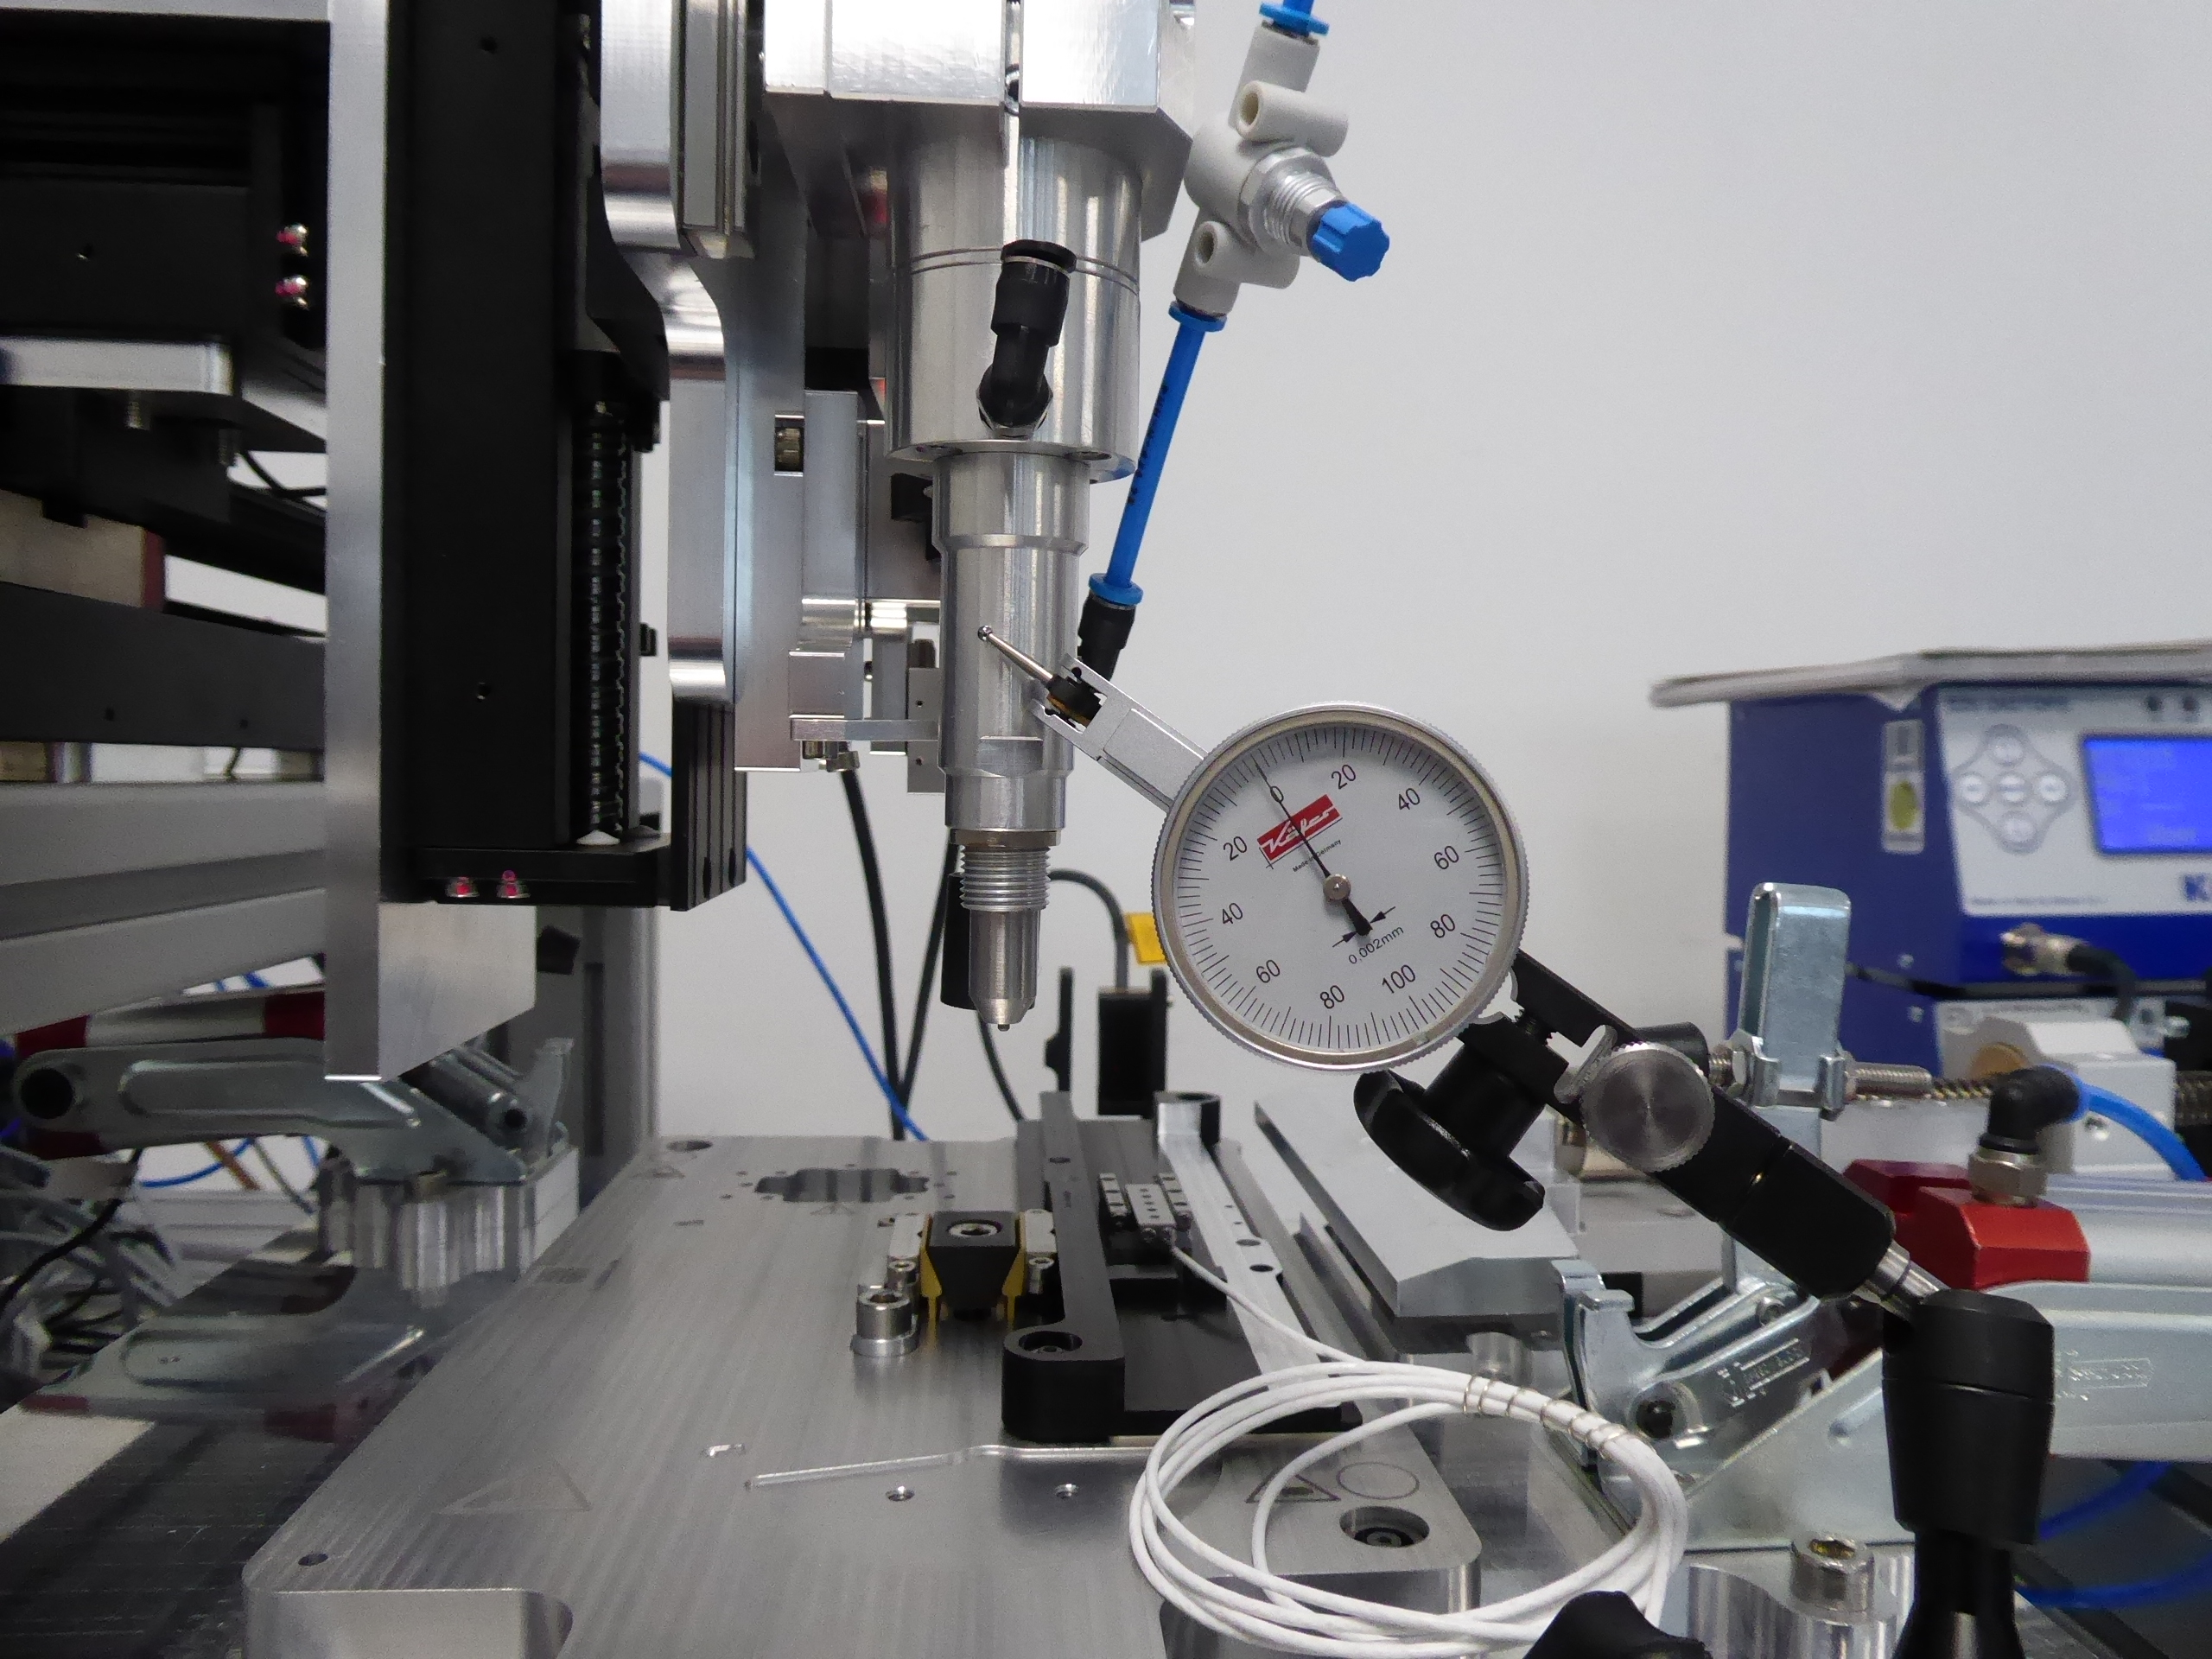
\includegraphics[width=\textwidth]{Bilder/06_Ergebnisse/x_start.JPG}
        \caption{Startposition der X-Achse}
        \label{fig:x_start}
    \end{subfigure}
    \hfill
    \begin{subfigure}[t]{0.45\textwidth}
        \centering
        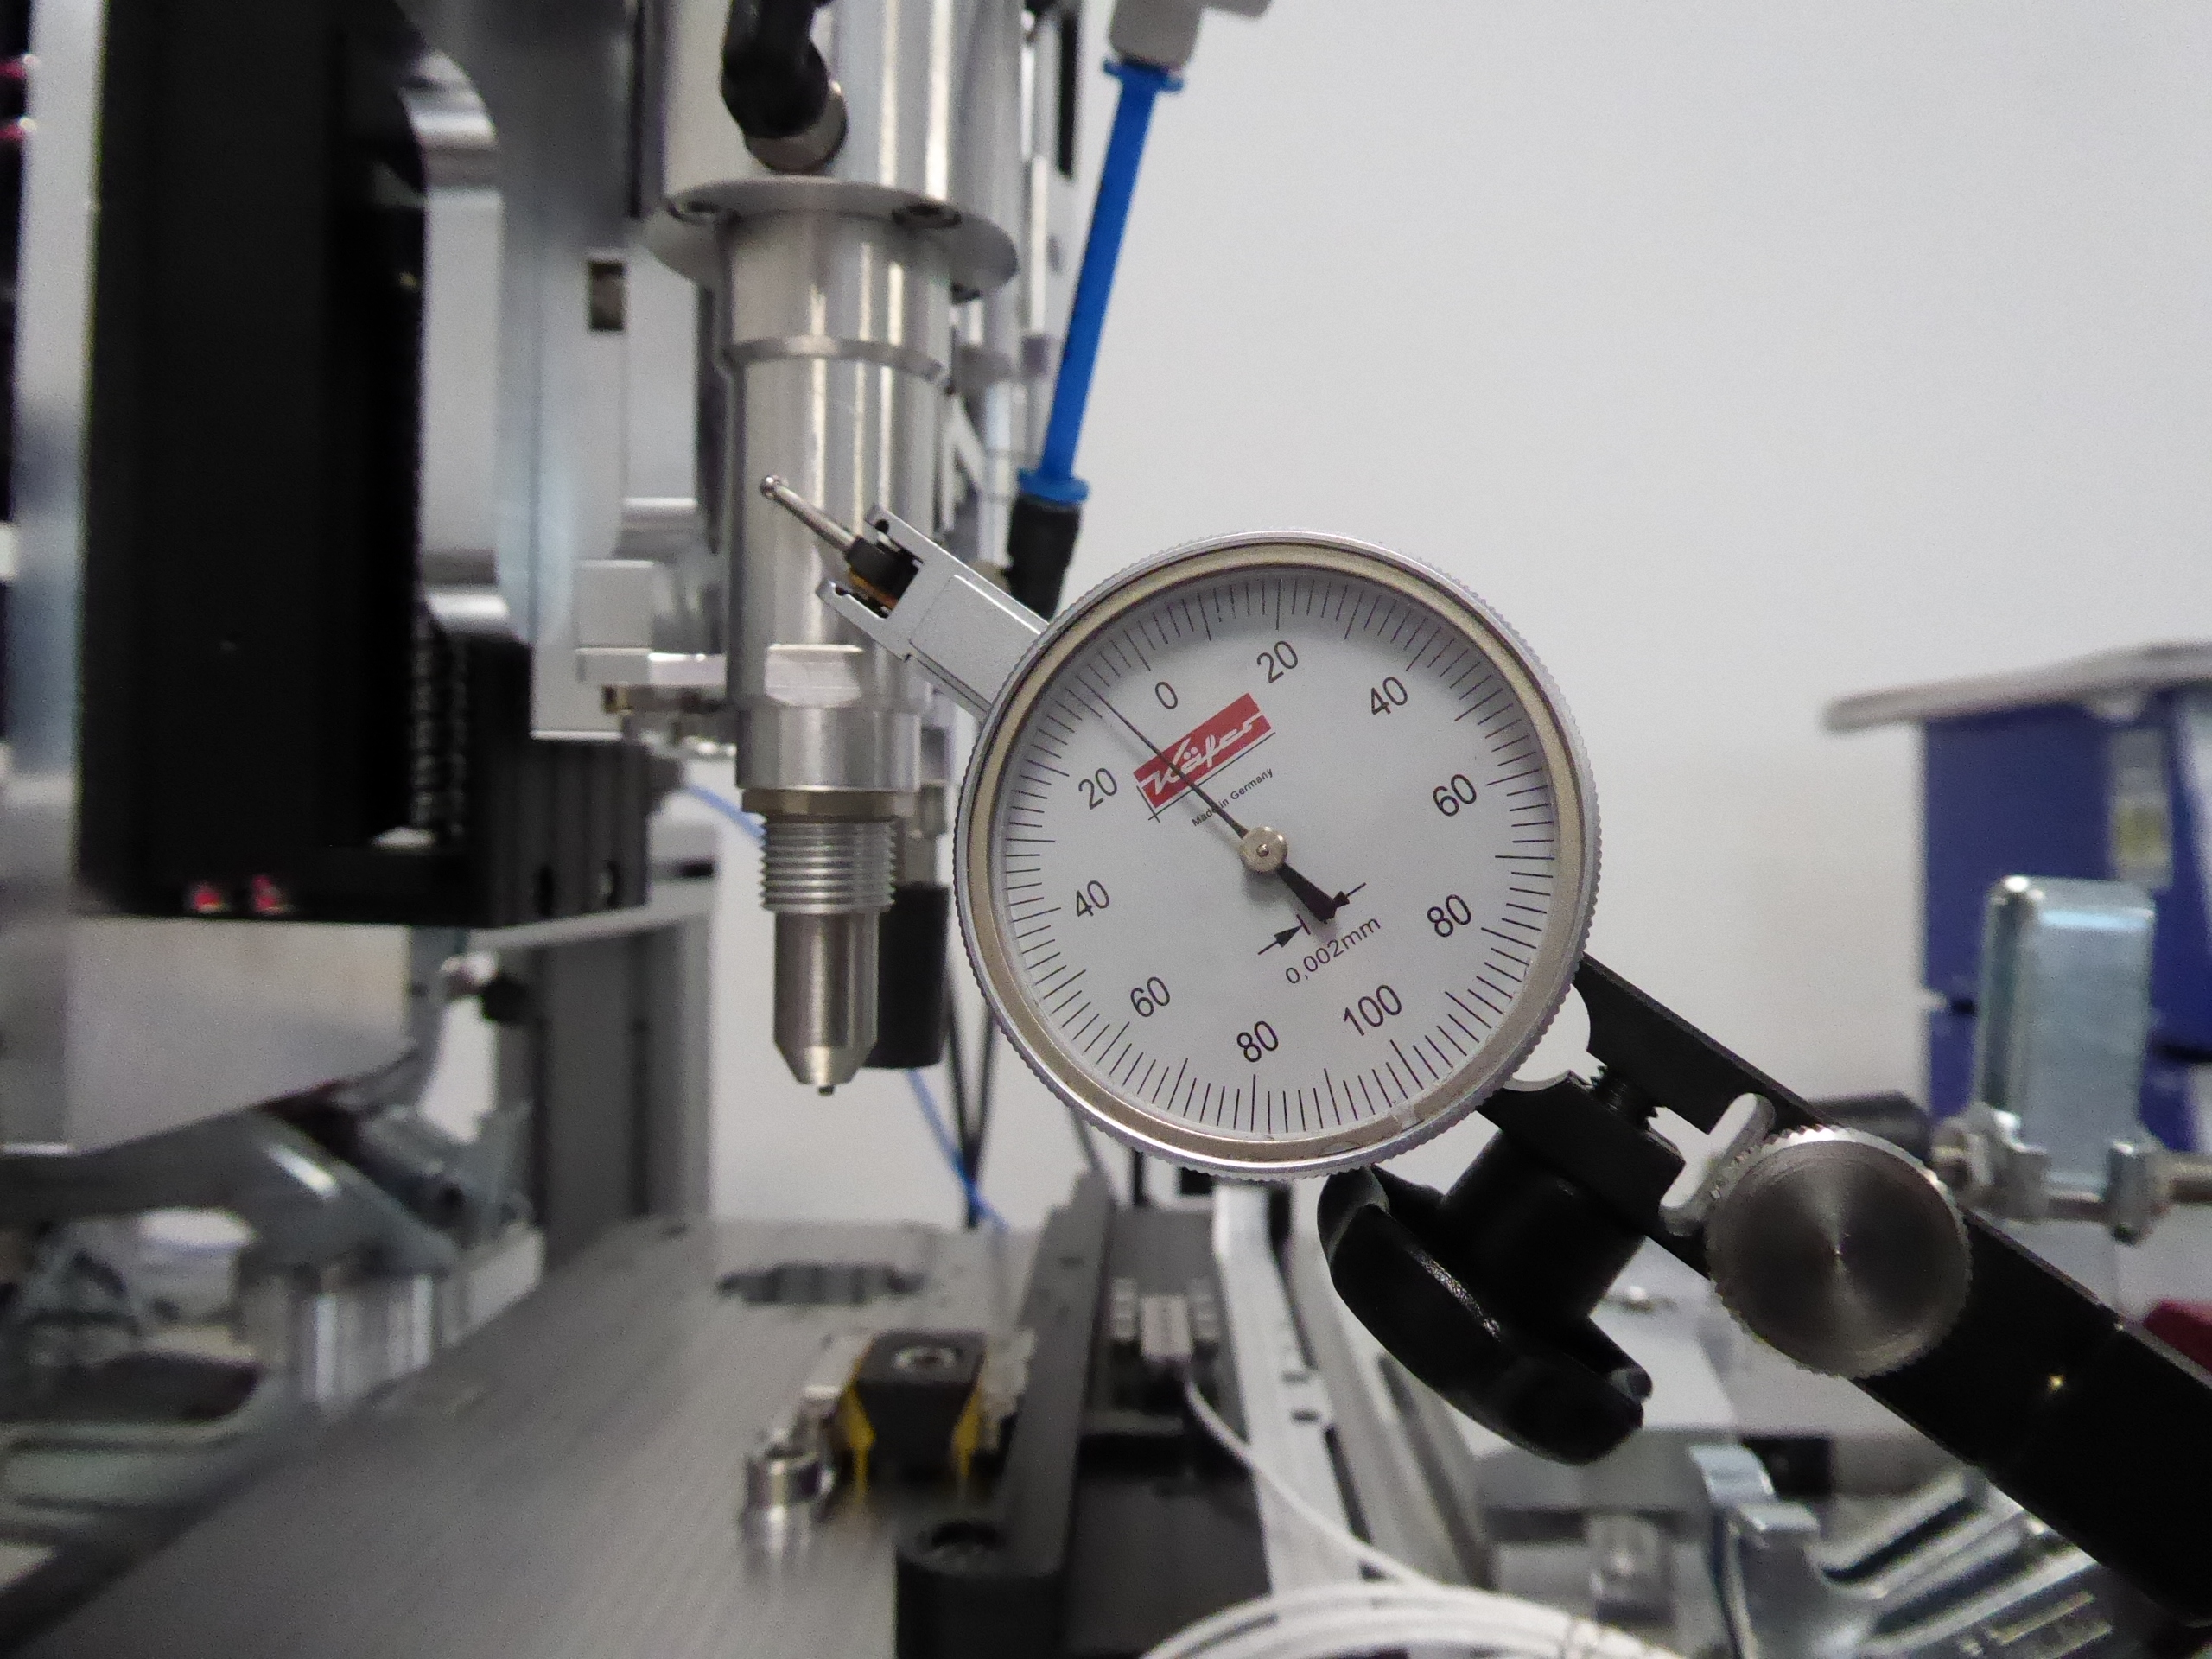
\includegraphics[width=\textwidth]{Bilder/06_Ergebnisse/x_end.JPG}
        \caption{Endposition der X-Achse}
        \label{fig:x_ende}
    \end{subfigure}

    \caption{Messaufbau zur Überprüfung der Wiederholgenauigkeit der X-Achse}
    \label{fig:x_achse_messung}
\end{figure}

\begin{figure}[H]
    \centering
    \begin{subfigure}[t]{0.45\textwidth}
        \centering
        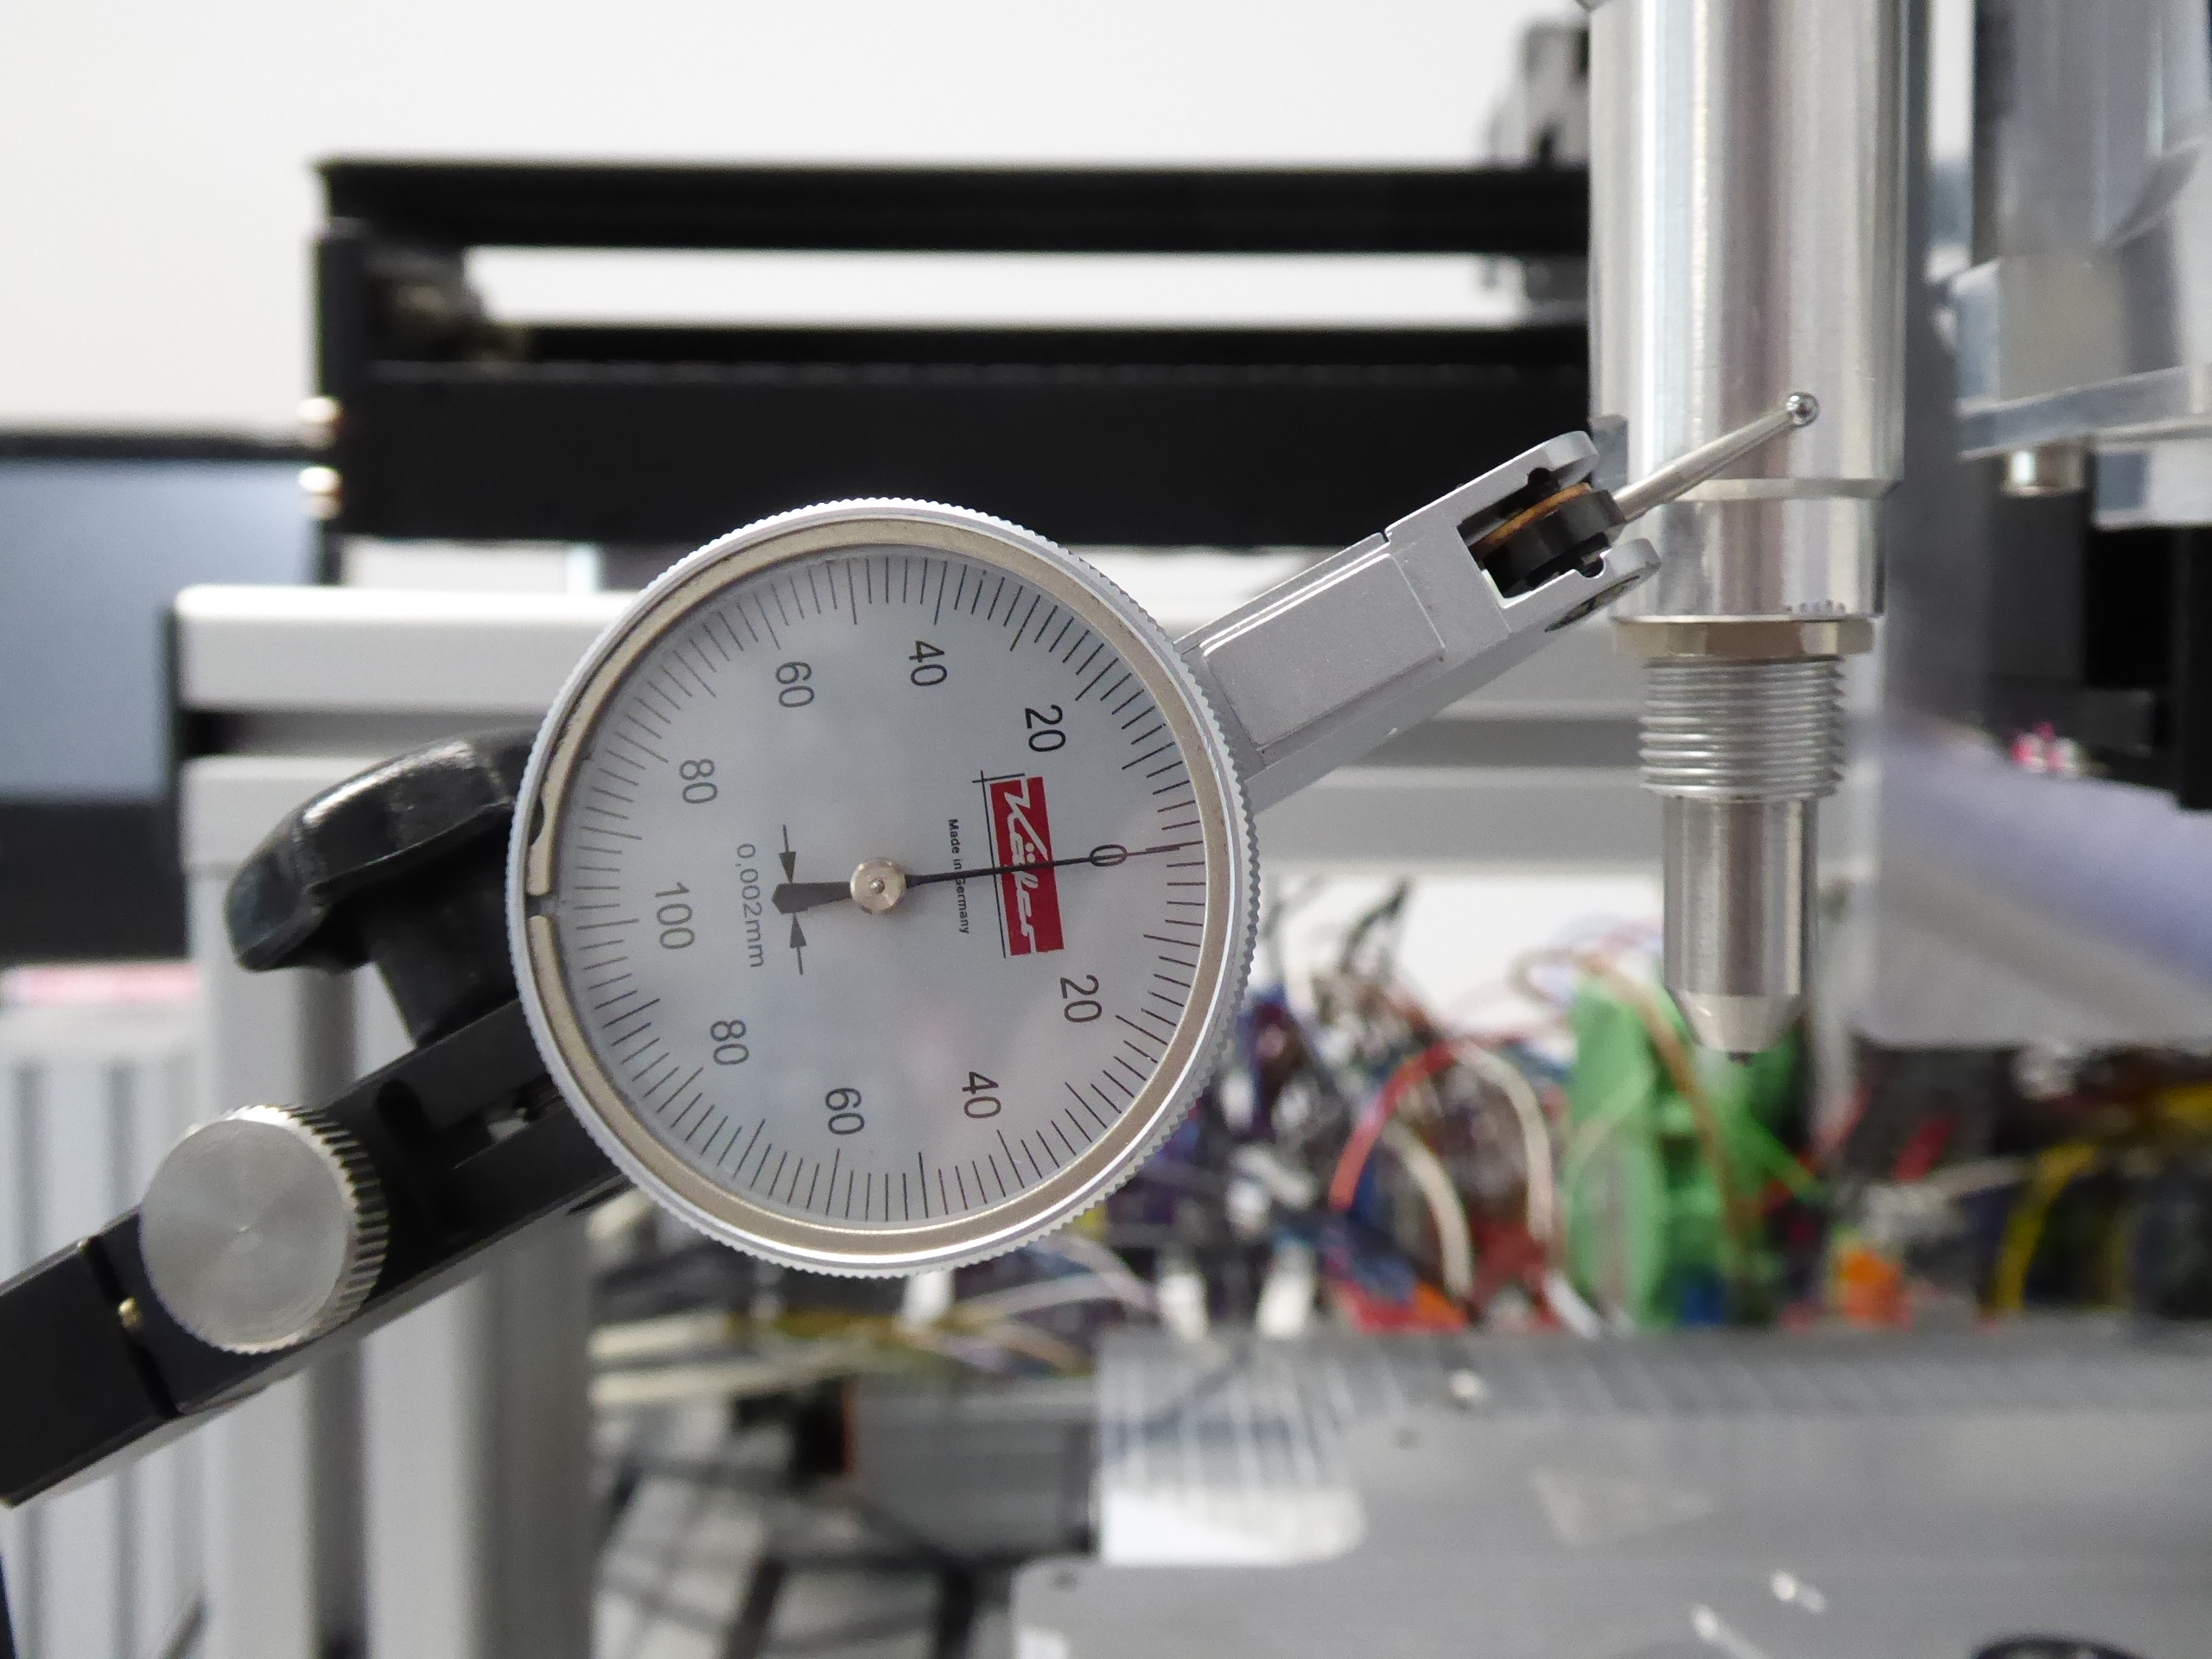
\includegraphics[width=\textwidth]{Bilder/06_Ergebnisse/y_start.JPG}
        \caption{Startposition der Y-Achse}
    \end{subfigure}
    \hfill
    \begin{subfigure}[t]{0.45\textwidth}
        \centering
        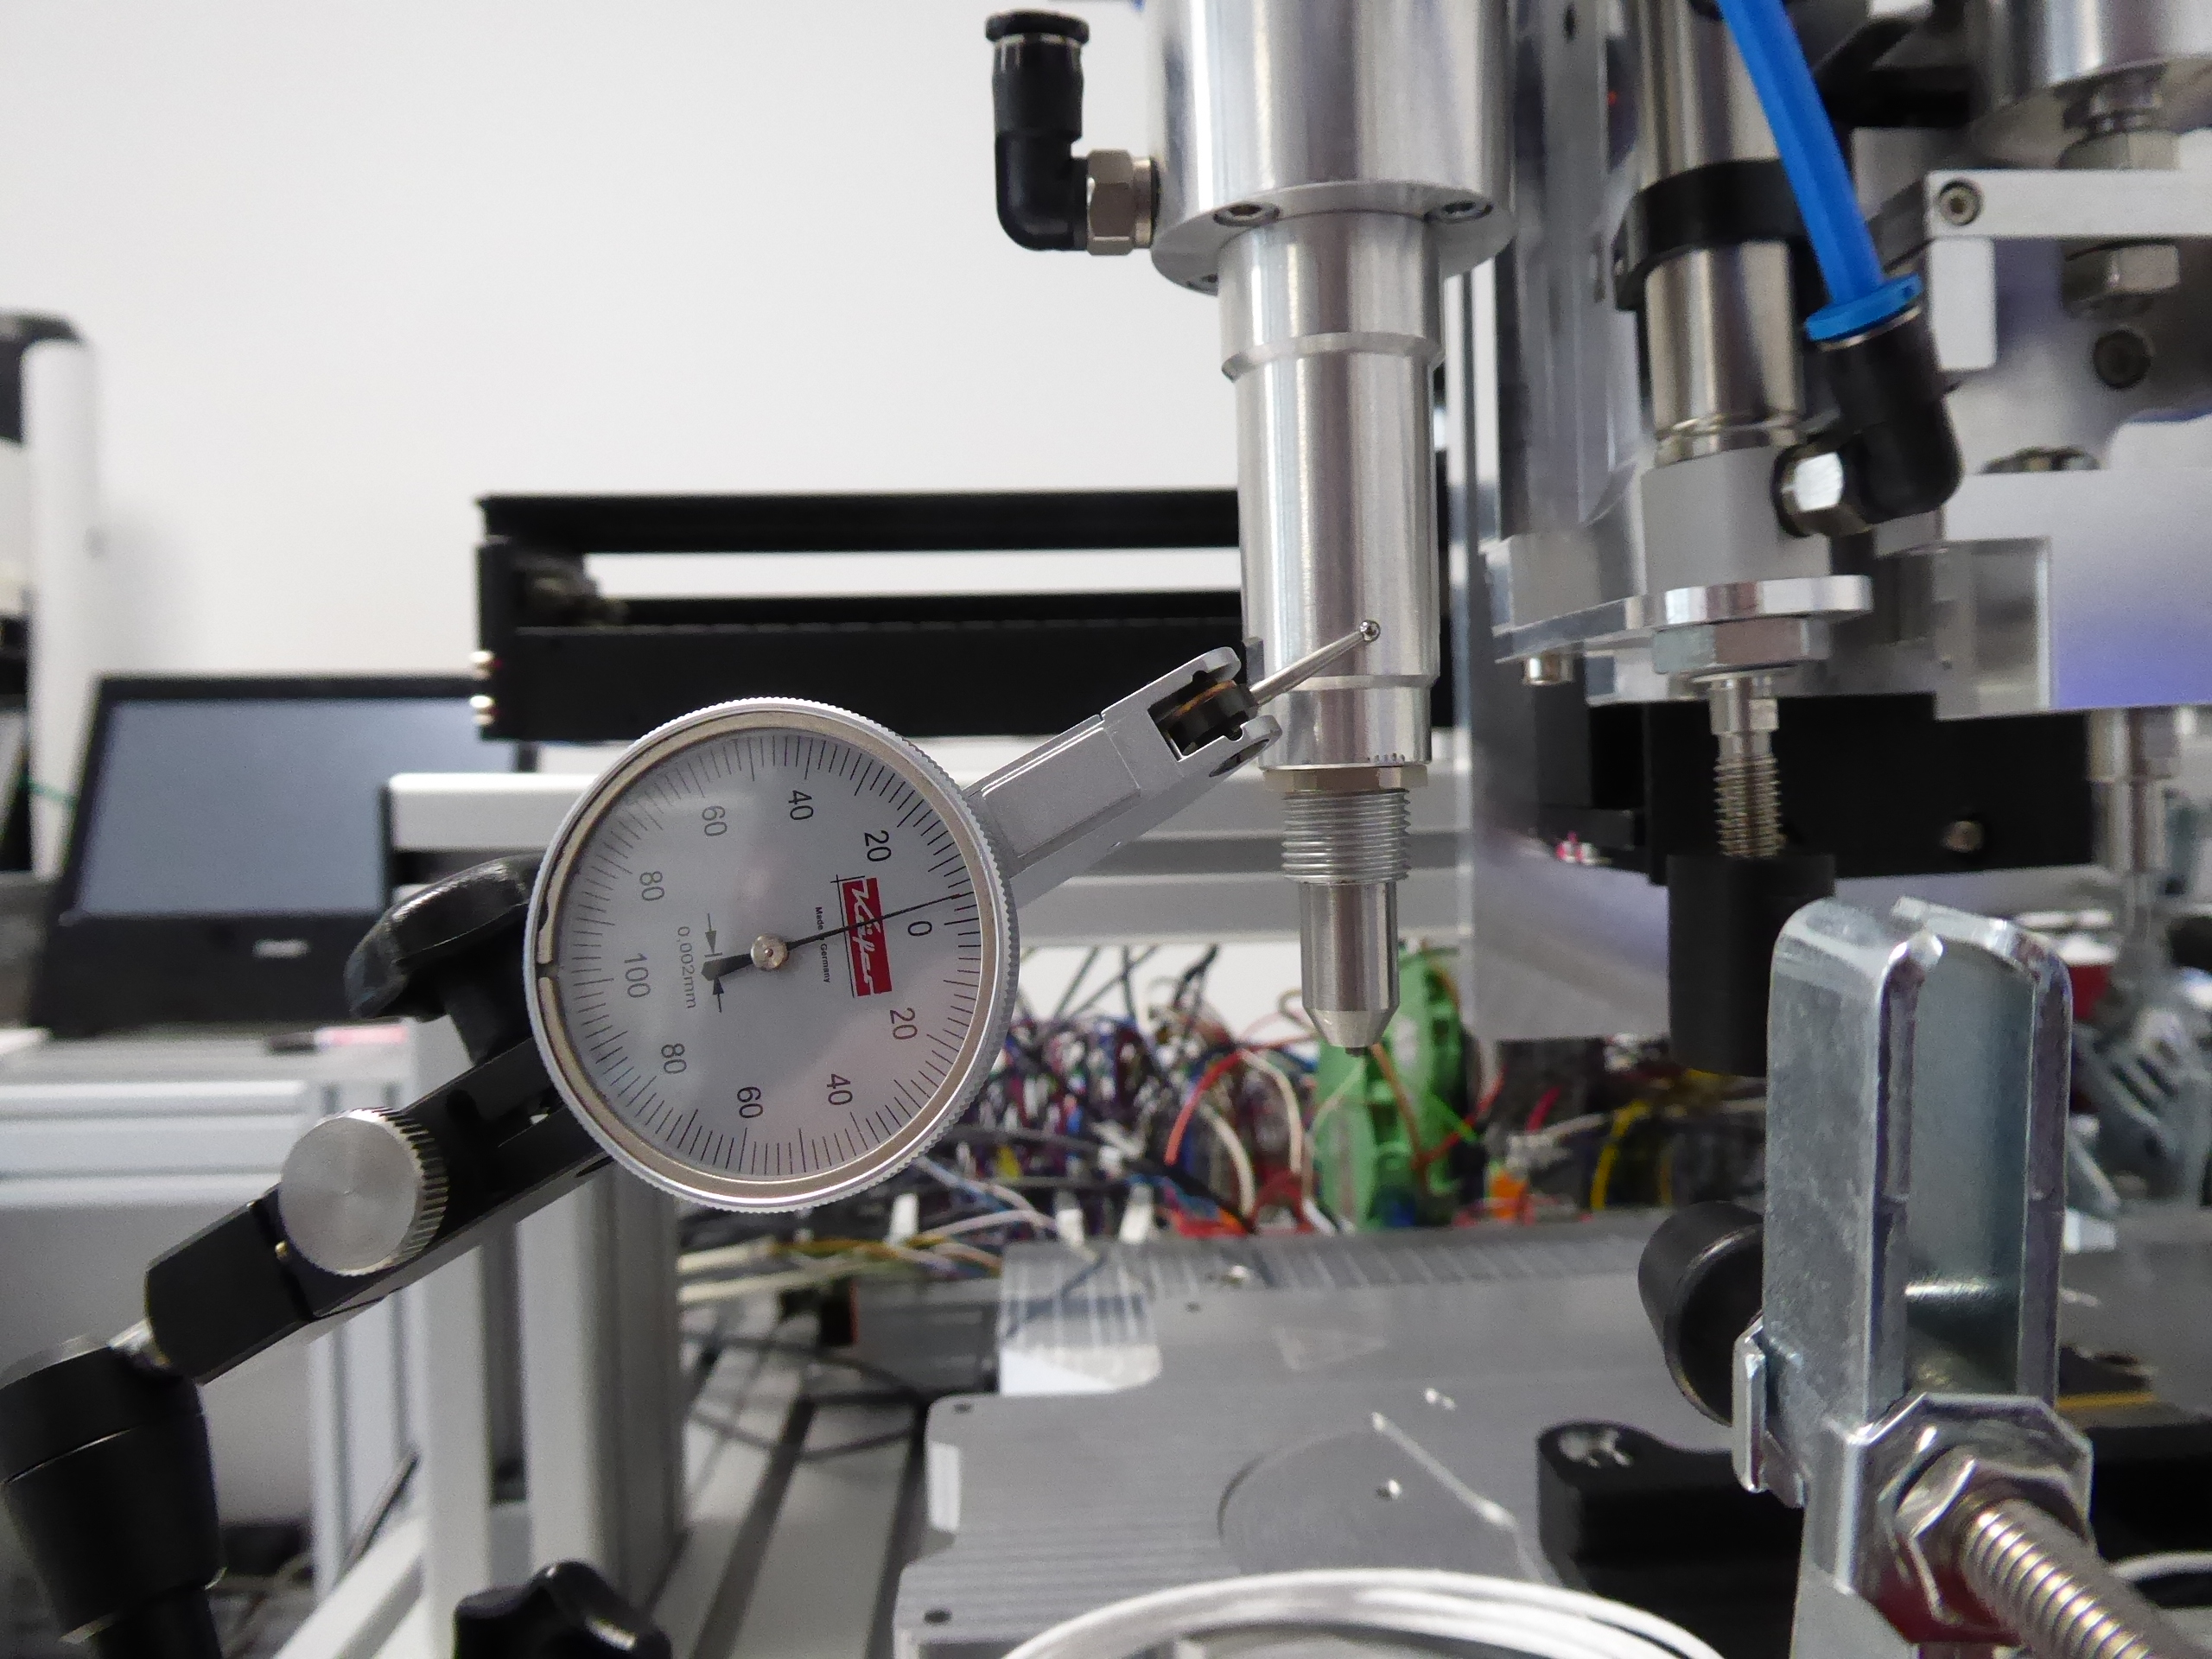
\includegraphics[width=\textwidth]{Bilder/06_Ergebnisse/y_end.JPG}
        \caption{Endposition der Y-Achse}
    \end{subfigure}

    \caption{Messaufbau zur Überprüfung der Wiederholgenauigkeit der Y-Achse}
    \label{fig:y_achse_messung}
\end{figure}

\begin{figure}[H]
    \centering
    \begin{subfigure}[t]{0.45\textwidth}
        \centering
        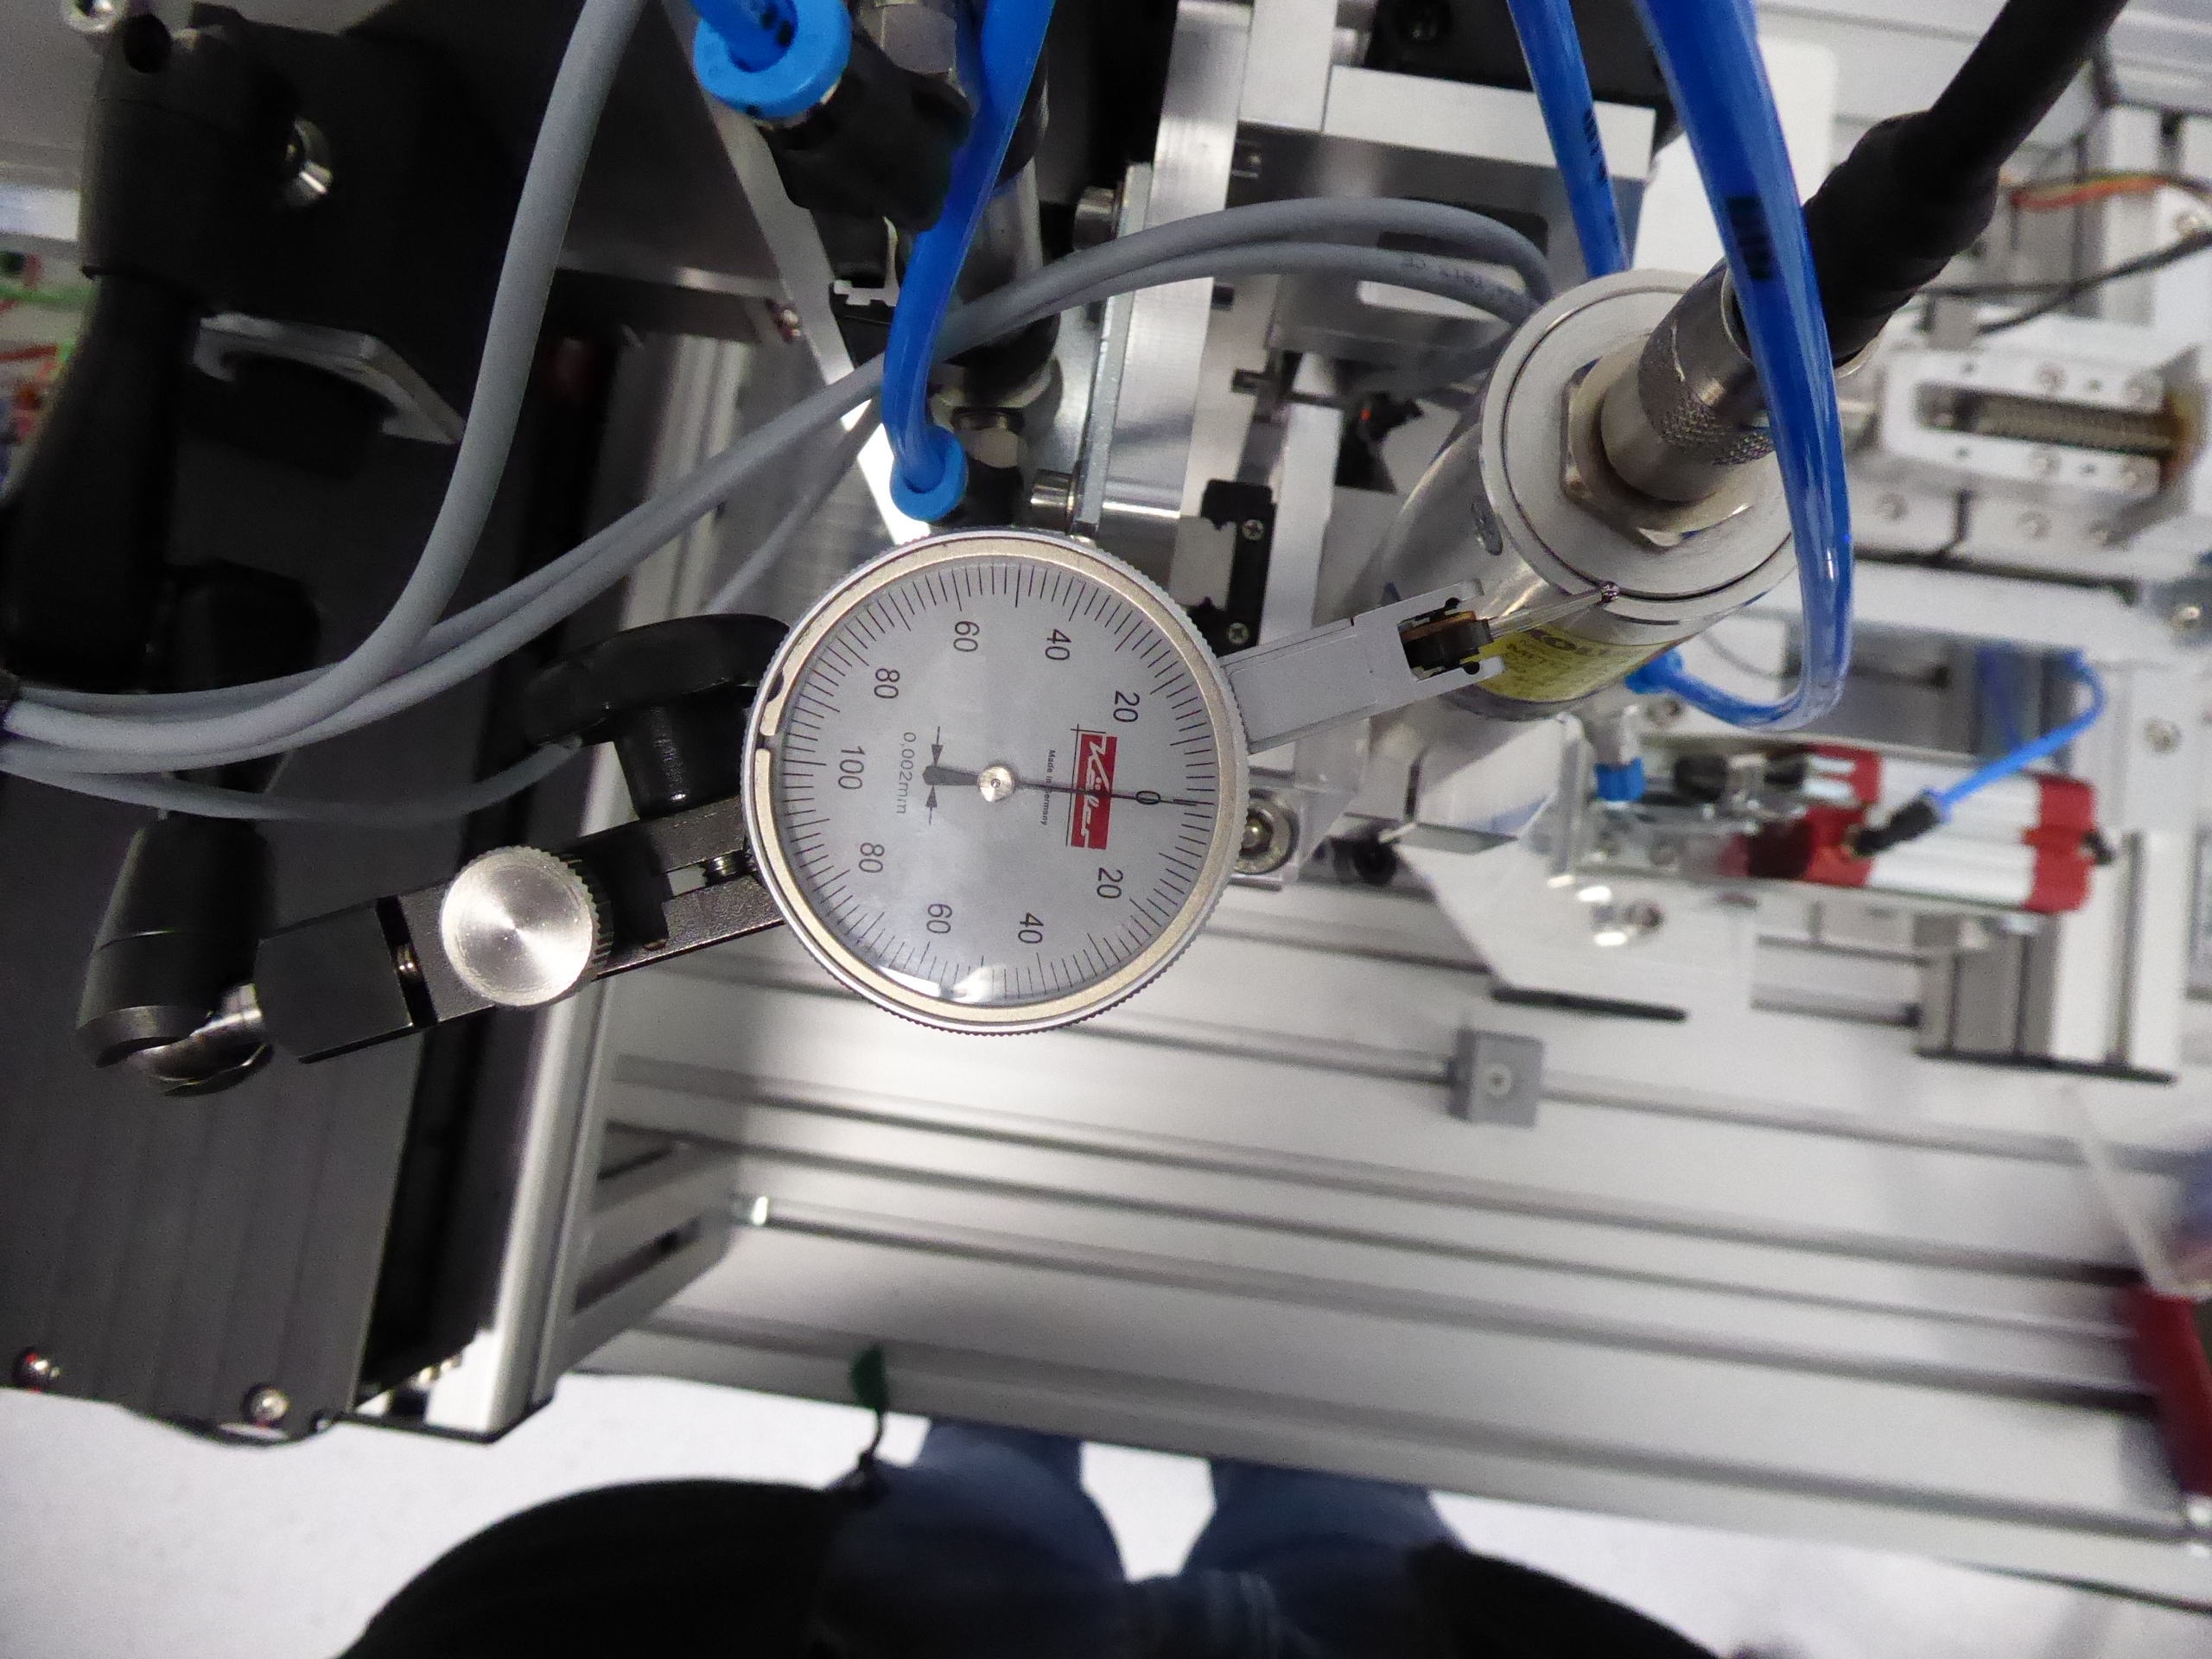
\includegraphics[width=\textwidth]{Bilder/06_Ergebnisse/z_start.JPG}
        \caption{Startposition der Z-Achse}
    \end{subfigure}
    \hfill
    \begin{subfigure}[t]{0.45\textwidth}
        \centering
        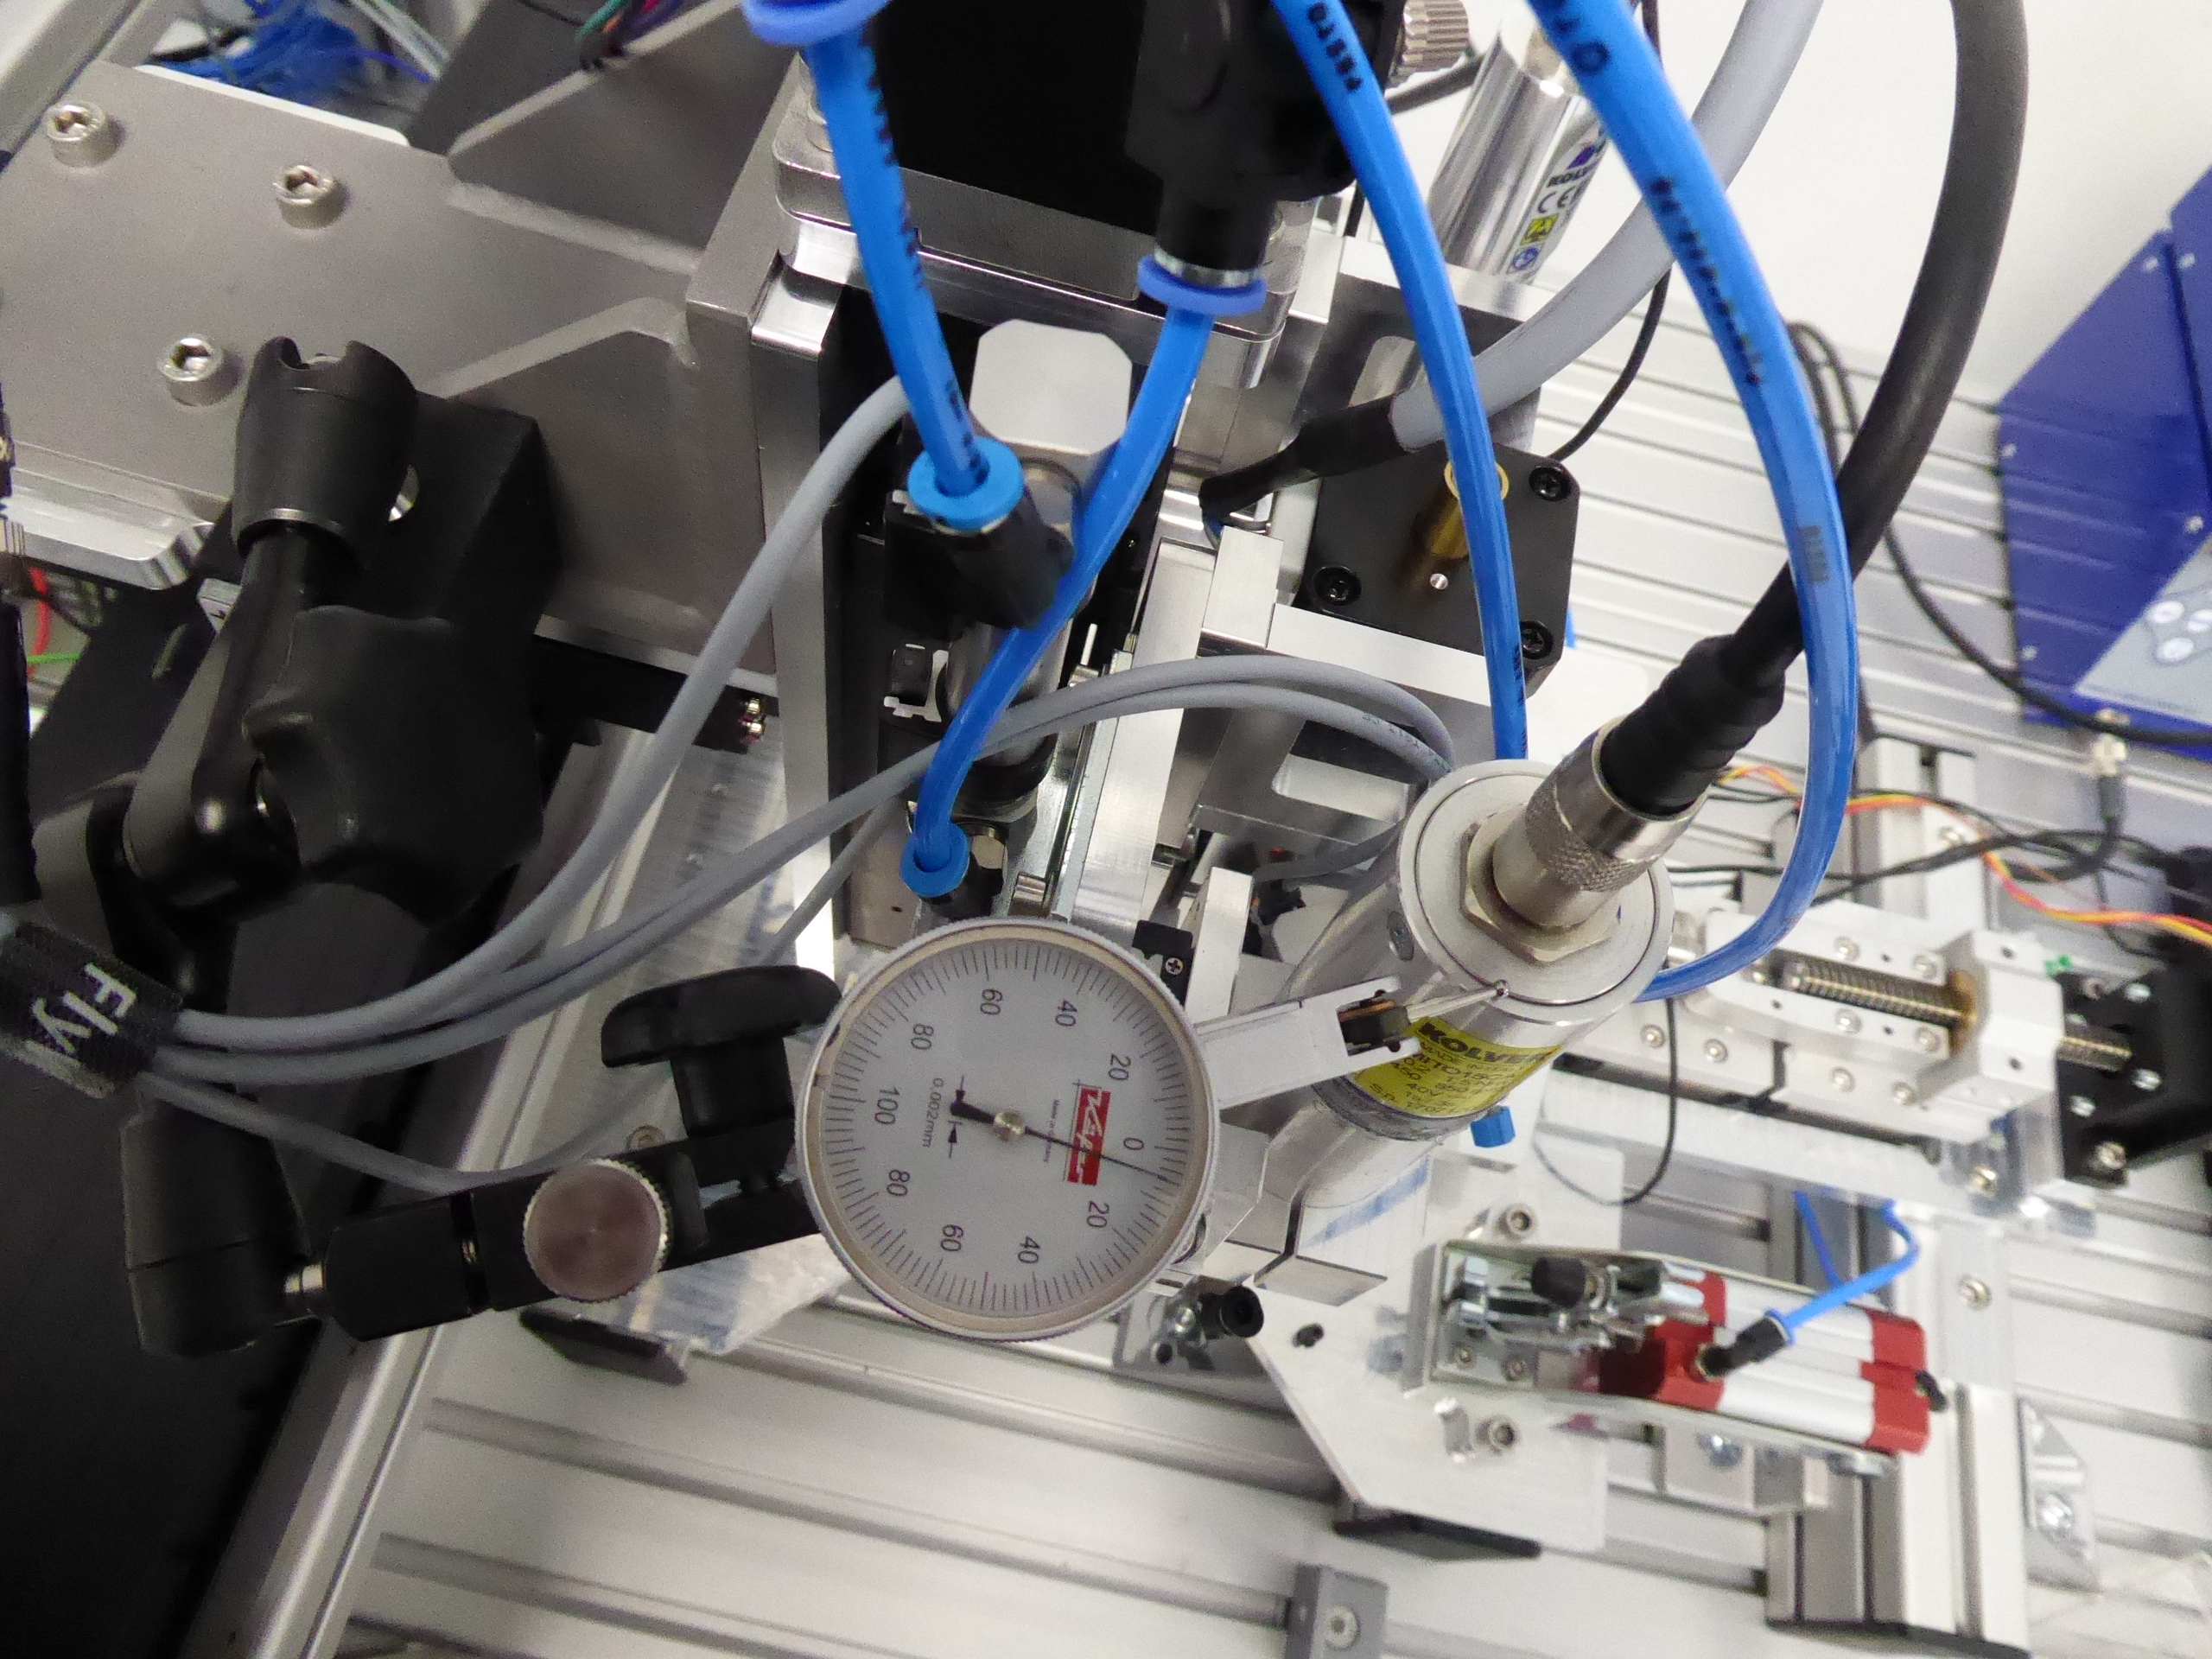
\includegraphics[width=\textwidth]{Bilder/06_Ergebnisse/z_end.JPG}
        \caption{Endposition der Z-Achse}
    \end{subfigure}

    \caption{Messaufbau zur Überprüfung der Wiederholgenauigkeit der Z-Achse}
    \label{fig:z_achse_messung}
\end{figure}

\subsubsection{Tests der Magnetventile und Näherungssensoren}
Die Magnetventile wurden manuell durch Ein- und Ausschalten angesteuert. Dabei wurde überprüft, ob die zugehörigen Näherungssensoren die jeweilige Endlage des Kolbens richtig erfassen. Sowohl die obere als auch die untere Endposition wurden zuverlässig erkannt.

Die Rückmeldungen der Sensoren waren eindeutig und stabil. Damit konnte die korrekte Funktion der Magnetventile in Kombination mit der Endlagensensorik bestätigt werden.

Die Abbildungen~\ref{fig:magnetventil_unten} und~\ref{fig:magnetventil_oben} zeigen die Umschaltung der Näherungssensoren zwischen der unteren und oberen Endlage der Rundkolbenzylinder in Abhängigkeit von der Ventilansteuerung.

\begin{figure}[H]
    \centering
    \begin{subfigure}[t]{0.48\textwidth}
        \centering
        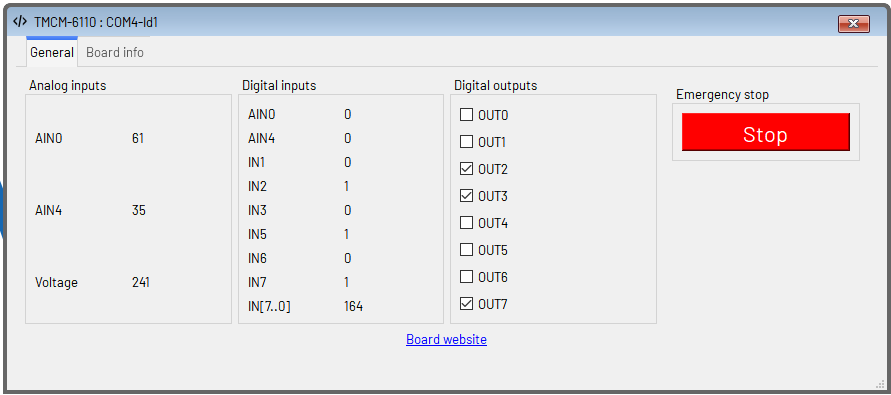
\includegraphics[width=\textwidth]{Bilder/06_Ergebnisse/ventile_an.png}
        \caption{Untere Endlage des Kolbens}
        \label{fig:magnetventil_unten}
    \end{subfigure}
    \hfill
    \begin{subfigure}[t]{0.48\textwidth}
        \centering
        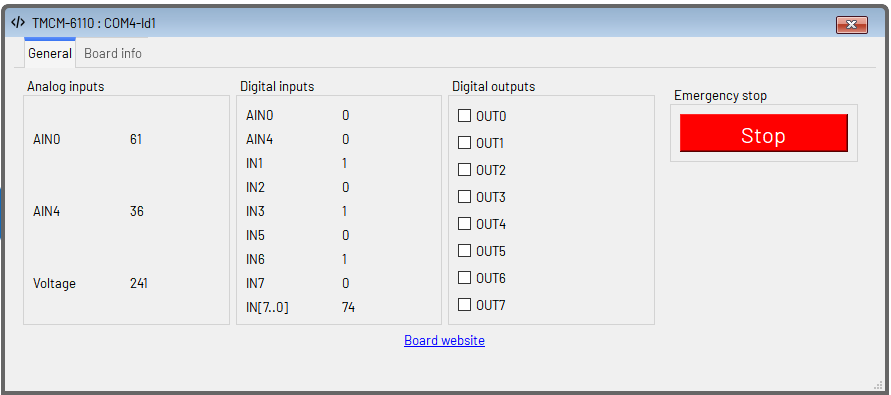
\includegraphics[width=\textwidth]{Bilder/06_Ergebnisse/ventile_aus.png}
        \caption{Obere Endlage des Kolbens}
        \label{fig:magnetventil_oben}
    \end{subfigure}

    \caption{Anzeige der digitalen Ein- und Ausgangssignale während der Ansteuerung der Magnetventile im TMCL-IDE}
    \label{fig:magnetventil_tmcl}
\end{figure}

\subsubsection{Tests der Kraftmessdosen}
Die Kraftmessdosen wurden manuell belastet, um die Signalreaktion zu überprüfen. Die ausgegebenen Messwerte reagierten nachvollziehbar auf Laständerungen und zeigten ein stabiles Verhalten. Die Tara-Funktion arbeitete zuverlässig.

Ein geringes Rauschen war im Signal erkennbar. Da die Kraftmessdosen während der Tests noch nicht vollständig mechanisch fixiert waren, ist dieses Verhalten als unkritisch zu bewerten. Die grundsätzliche Funktionsfähigkeit der Kraftmessdosen konnte bestätigt werden.

Wie in Abbildung~\ref{fig:kmd_rauschen} dargestellt, ist im unbelasteten Zustand der Kraftmessdosen ein geringes Rauschen der Messwerte erkennbar. Dieses Verhalten ist auf den noch nicht vollständig fixierten mechanischen Aufbau während der Tests zurückzuführen und wird als unkritisch bewertet.

Bei manueller Belastung der Kraftmessdosen zeigen die Messwerte eine eindeutige und reproduzierbare Änderung, wie in den Abbildungen~\ref{fig:kmd_belastet_1} und~\ref{fig:kmd_belastet_2} zu sehen ist. Der jeweilige Belastungszustand wird zusätzlich über die digitalen Eingänge korrekt signalisiert, wodurch die Funktion der Kraftmessdosen bestätigt werden kann.

\begin{figure}[H]
    \centering
    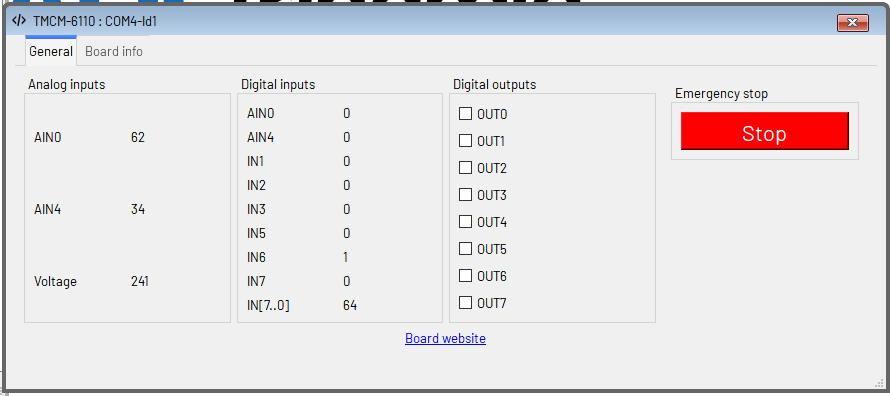
\includegraphics[width=0.7\textwidth]{Bilder/06_Ergebnisse/kmd_unbelastet.png}
    \caption{Messwertanzeige der Kraftmessdosen im unbelasteten Zustand mit erkennbaren Rauschanteilen}
    \label{fig:kmd_rauschen}
\end{figure}

\begin{figure}[H]
    \centering
    \begin{subfigure}[t]{0.48\textwidth}
        \centering
        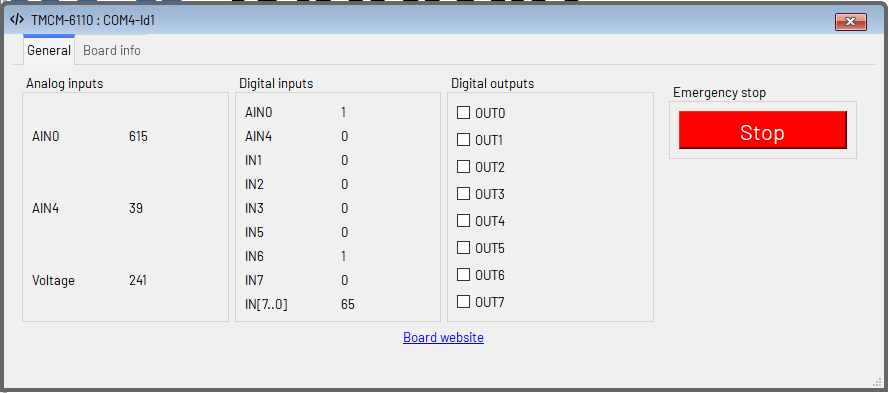
\includegraphics[width=\textwidth]{Bilder/06_Ergebnisse/kmd_vorspann.png}
        \caption{Manuelle Belastung der Kraftmessdose im Vorspannsystem}
        \label{fig:kmd_belastet_1}
    \end{subfigure}
    \hfill
    \begin{subfigure}[t]{0.48\textwidth}
        \centering
        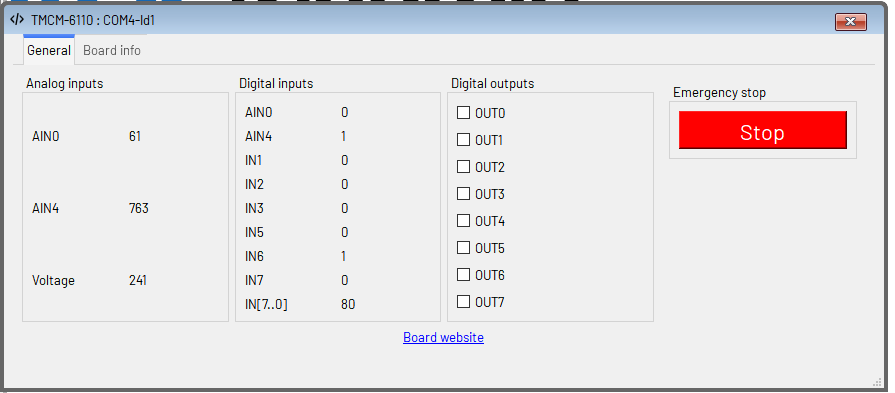
\includegraphics[width=\textwidth]{Bilder/06_Ergebnisse/kmd_keile.png}
        \caption{Manuelle Belastung der Kraftmessdose im Keile-Einpresssystem}
        \label{fig:kmd_belastet_2}
    \end{subfigure}

    \caption{Messwertänderung der Kraftmessdosen bei manueller Belastung mit zugehöriger digitaler Rückmeldung}
    \label{fig:kmd_belastet}
\end{figure}


\subsection{Durchgeführte Tests mit der WAGO-Steuerung}
\subsubsection{Tests der Laser-Triangulation Sensor}
Zur Überprüfung des Laser-Triangulationssensors wurde der Schlitten entlang der Messachse verfahren und der erfasste Abstand mit einer manuellen Referenzmessung verglichen. Die vom Sensor ausgegebenen Messwerte erwiesen sich als plausibel und reproduzierbar.

Die durchgeführten Tests zeigen, dass der Sensor zuverlässig arbeitet und für die Positions- und Abstandsüberwachung innerhalb des Systems geeignet ist.

\begin{figure}[H]
    \centering
    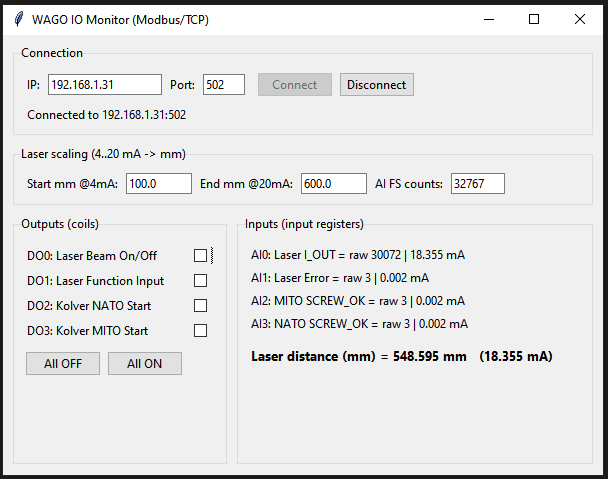
\includegraphics[width=0.85\textwidth]{Bilder/06_Ergebnisse/laser_distance.png}
    \caption{Ausgabe der Messwerte des Laser-Triangulationssensors im WAGO IO Monitor während der Verfahrbewegung des Schlittens}
    \label{fig:laser_wago}
\end{figure}

\subsubsection{Tests der automatische Schraubendreher}
Die automatischen Schraubendreher wurden hinsichtlich der Ansteuerung und Rückmeldung getestet. Start-, Stopp- und Statussignale wurden korrekt auf der Anzeige des EDU-Systems dargestellt. Auch Fehlversuche wurden zuverlässig angezeigt.

Bei Tests ohne eingesetzte Schraube zeigte sich, dass das Signal „Screw OK“ kurzzeitig auf den Wert~1 gesetzt wurde und anschließend wieder auf~0 zurückfiel. Dieses Verhalten trat ausschließlich bei Leerlauftests auf und ist auf den fehlenden realen Schraubprozess zurückzuführen.

\begin{figure}[H]
    \centering
    \begin{subfigure}[t]{0.32\textwidth}
        \centering
        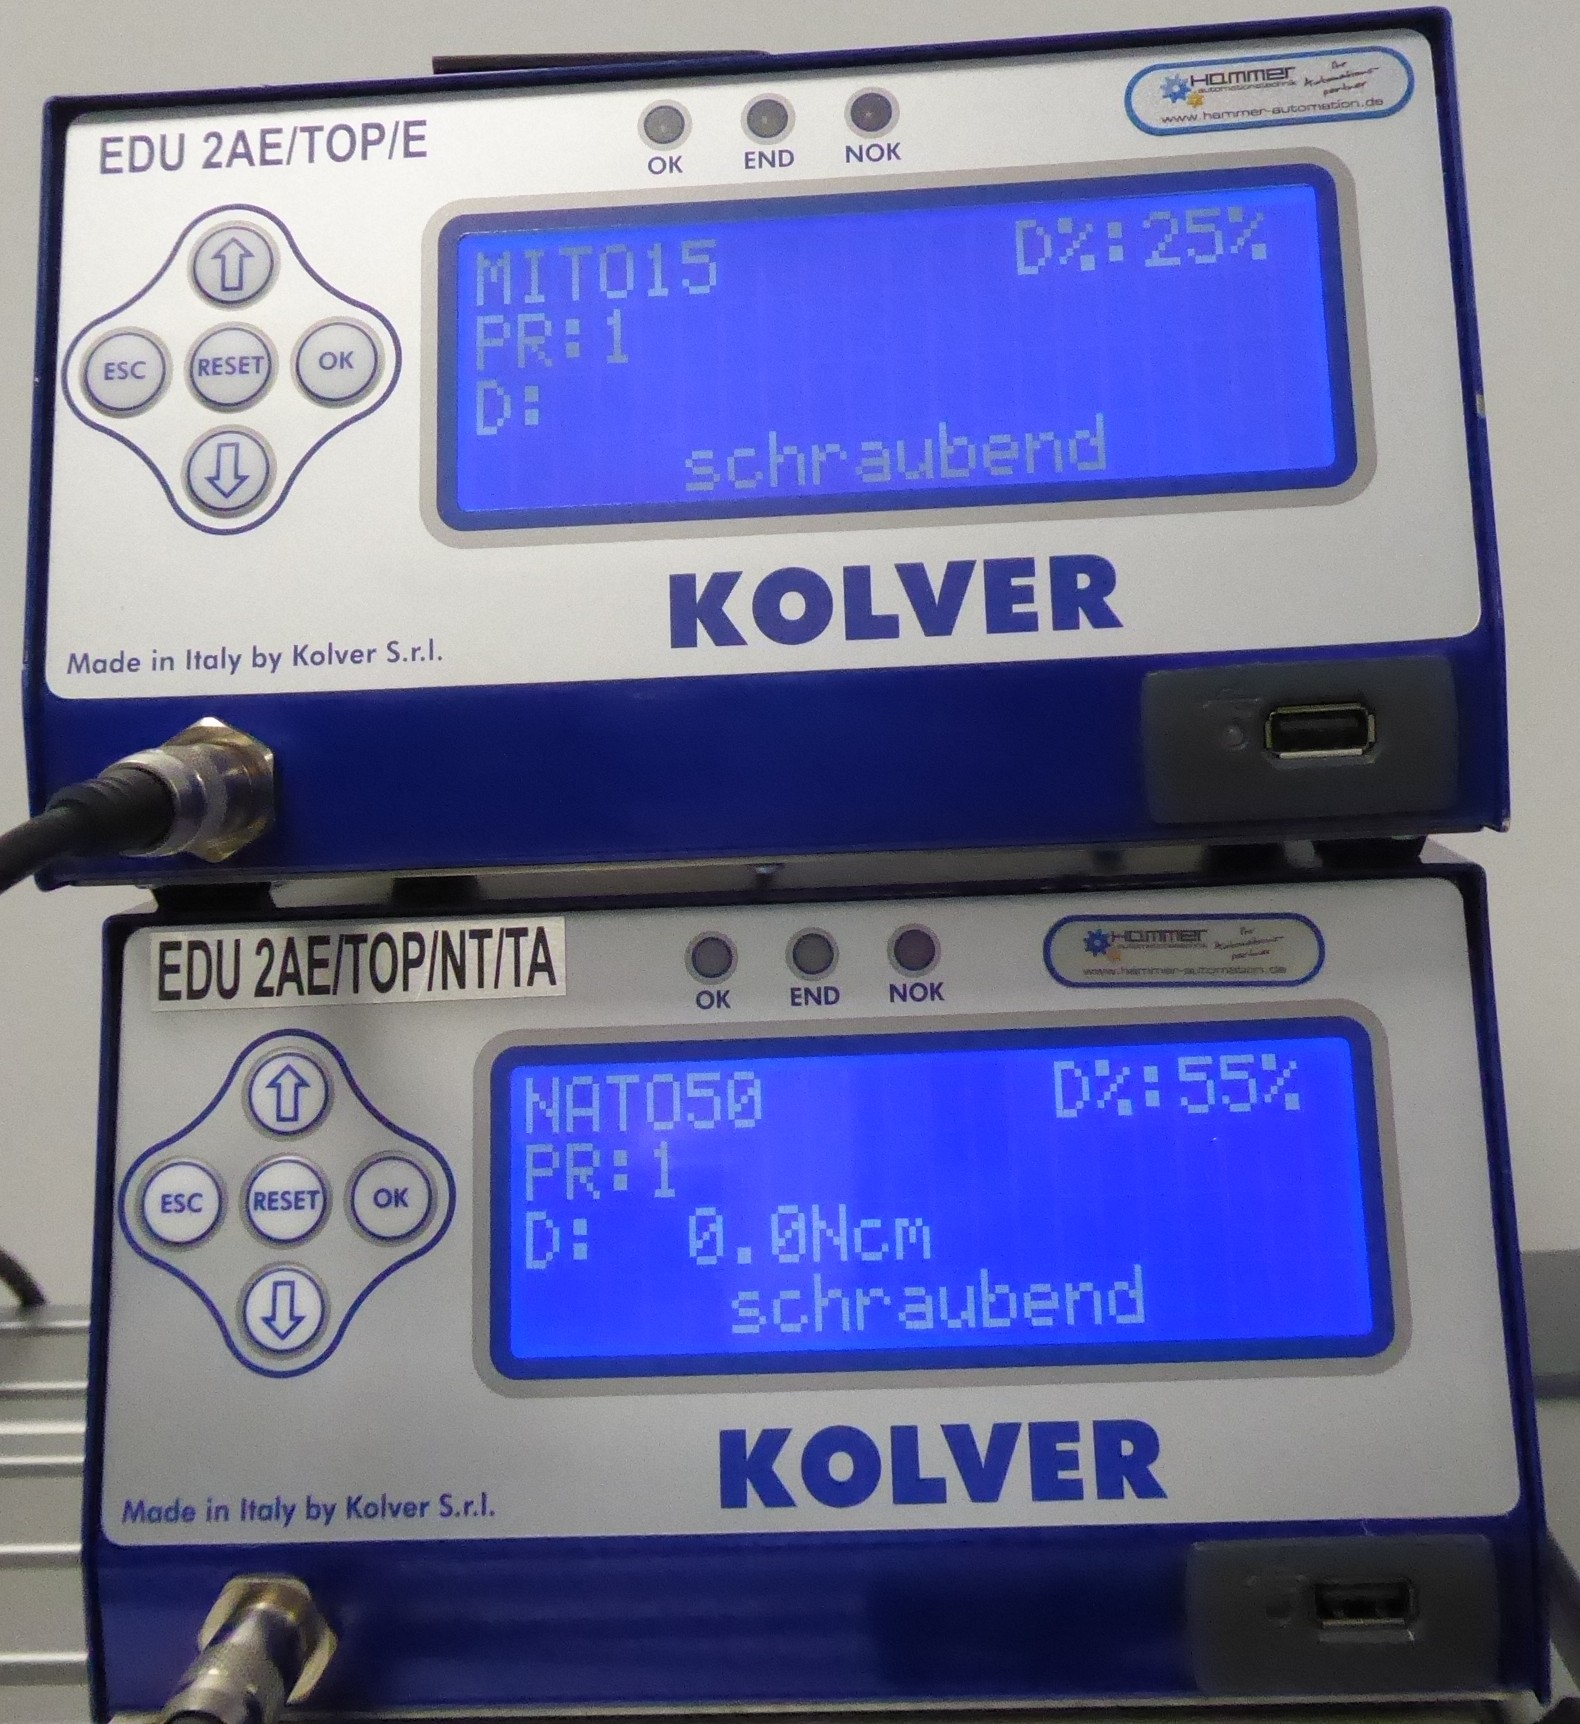
\includegraphics[width=\textwidth]{Bilder/06_Ergebnisse/kolver_init.JPG}
        \caption{Initialzustand der EDU-Anzeige}
        \label{fig:kolver_init}
    \end{subfigure}
    \hfill
    \begin{subfigure}[t]{0.32\textwidth}
        \centering
        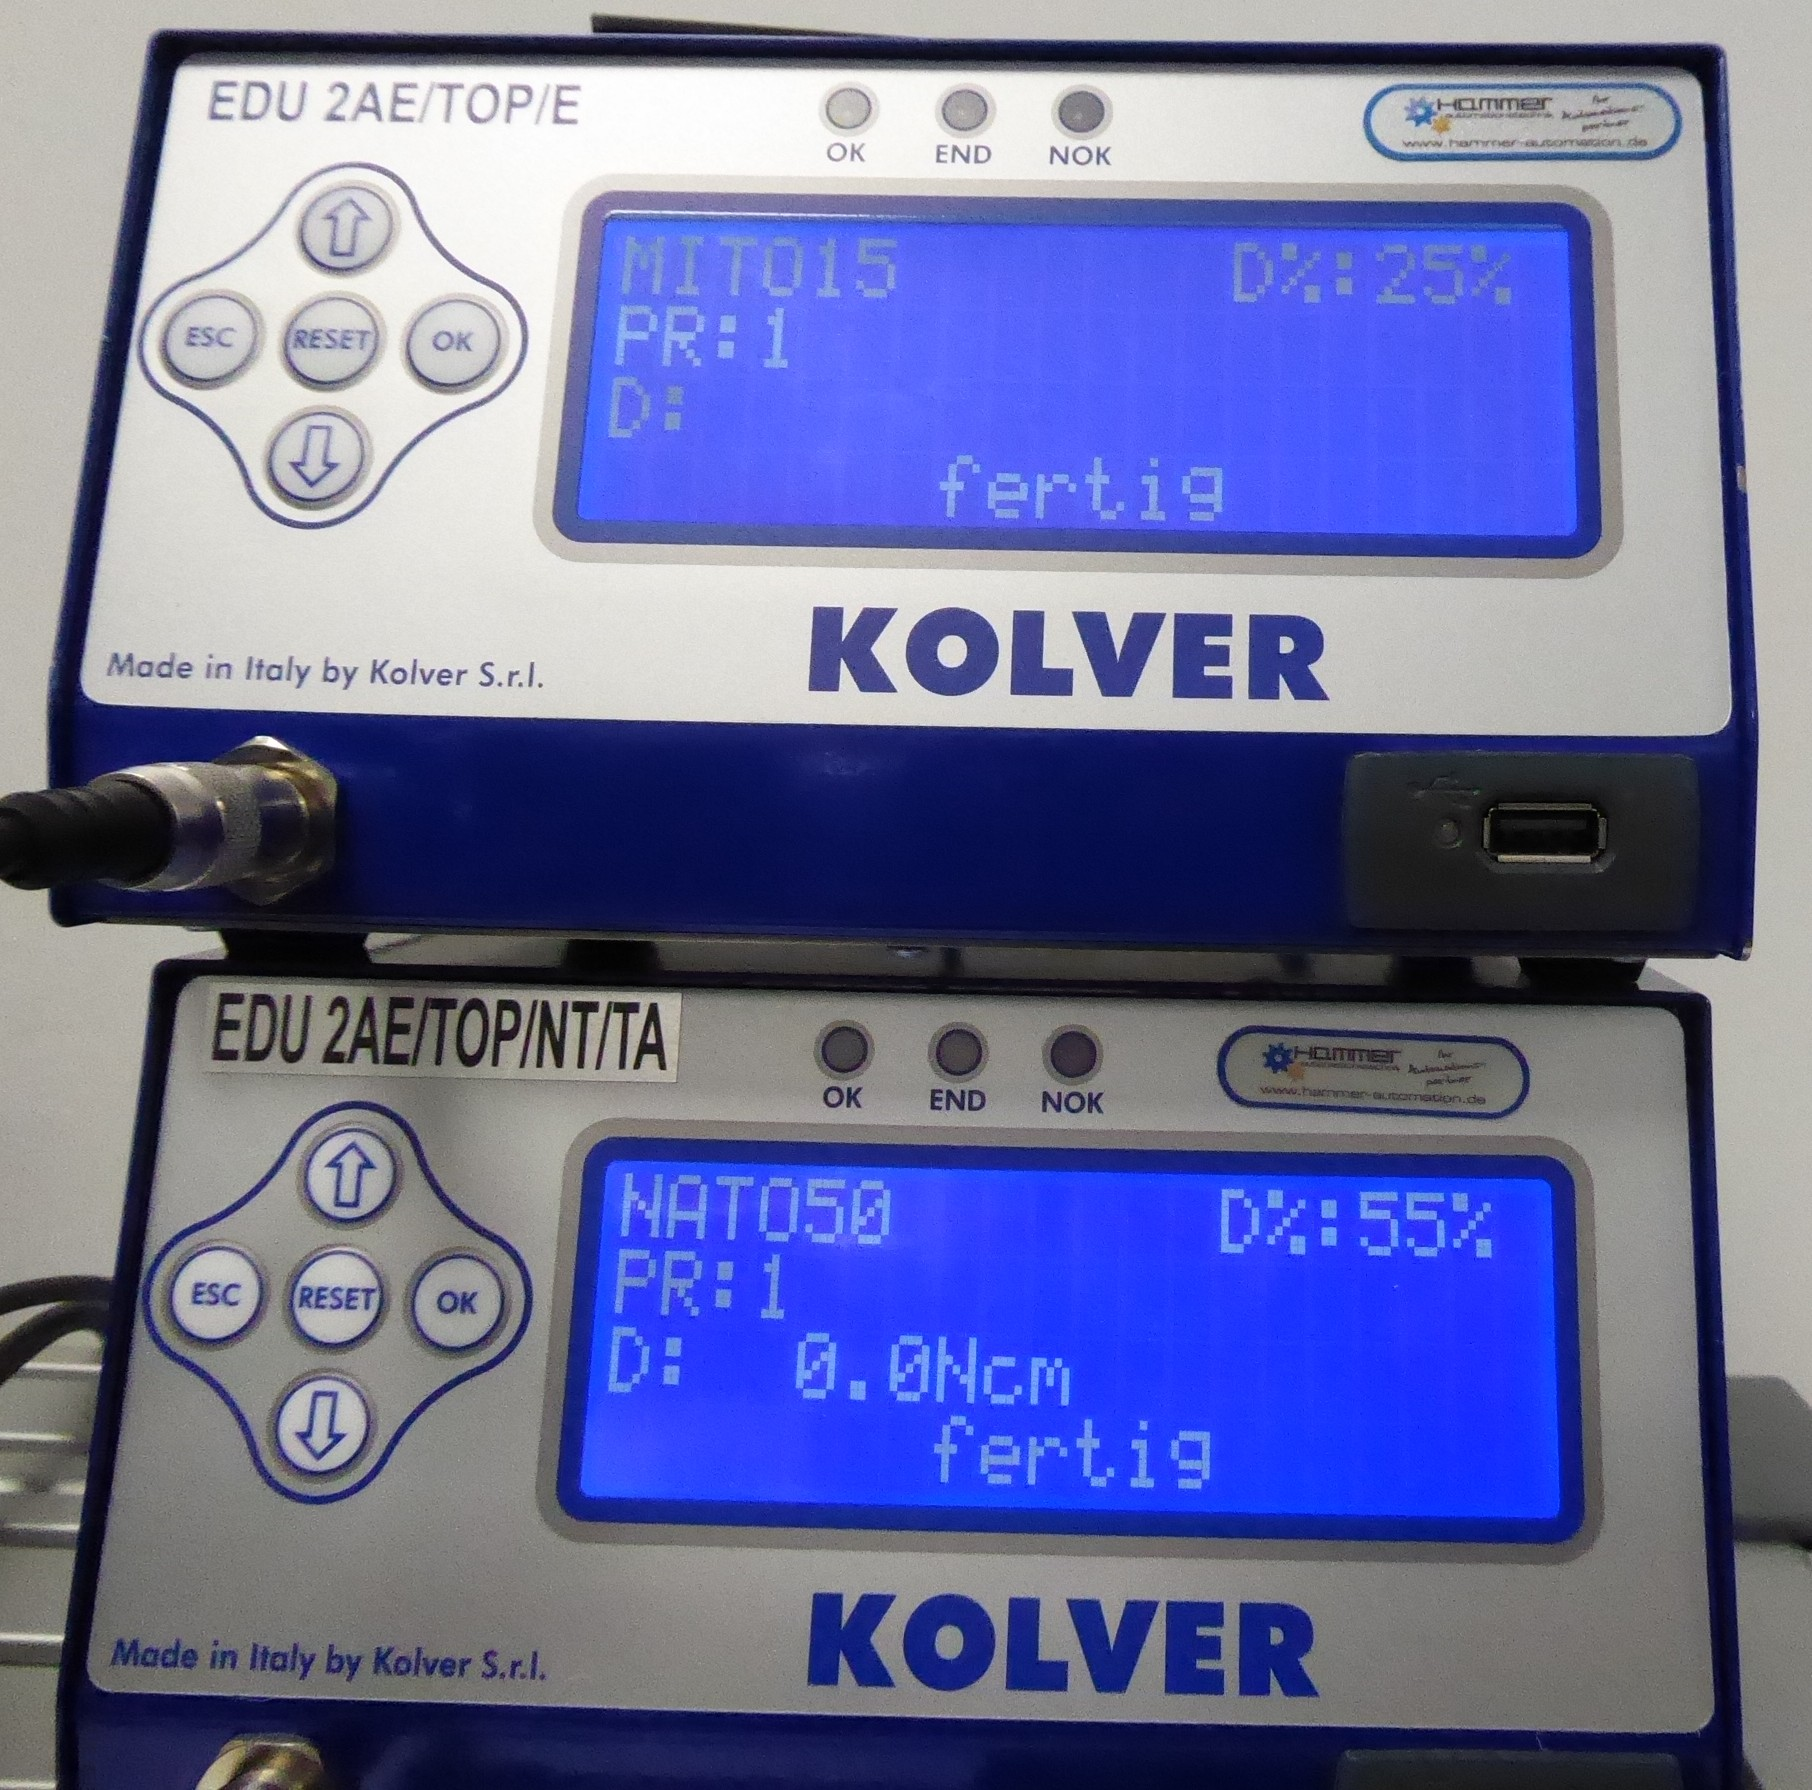
\includegraphics[width=\textwidth]{Bilder/06_Ergebnisse/kolver_ok.JPG}
        \caption{Erfolgreicher Verschrauben}
        \label{fig:kolver_ok}
    \end{subfigure}
    \hfill
    \begin{subfigure}[t]{0.32\textwidth}
        \centering
        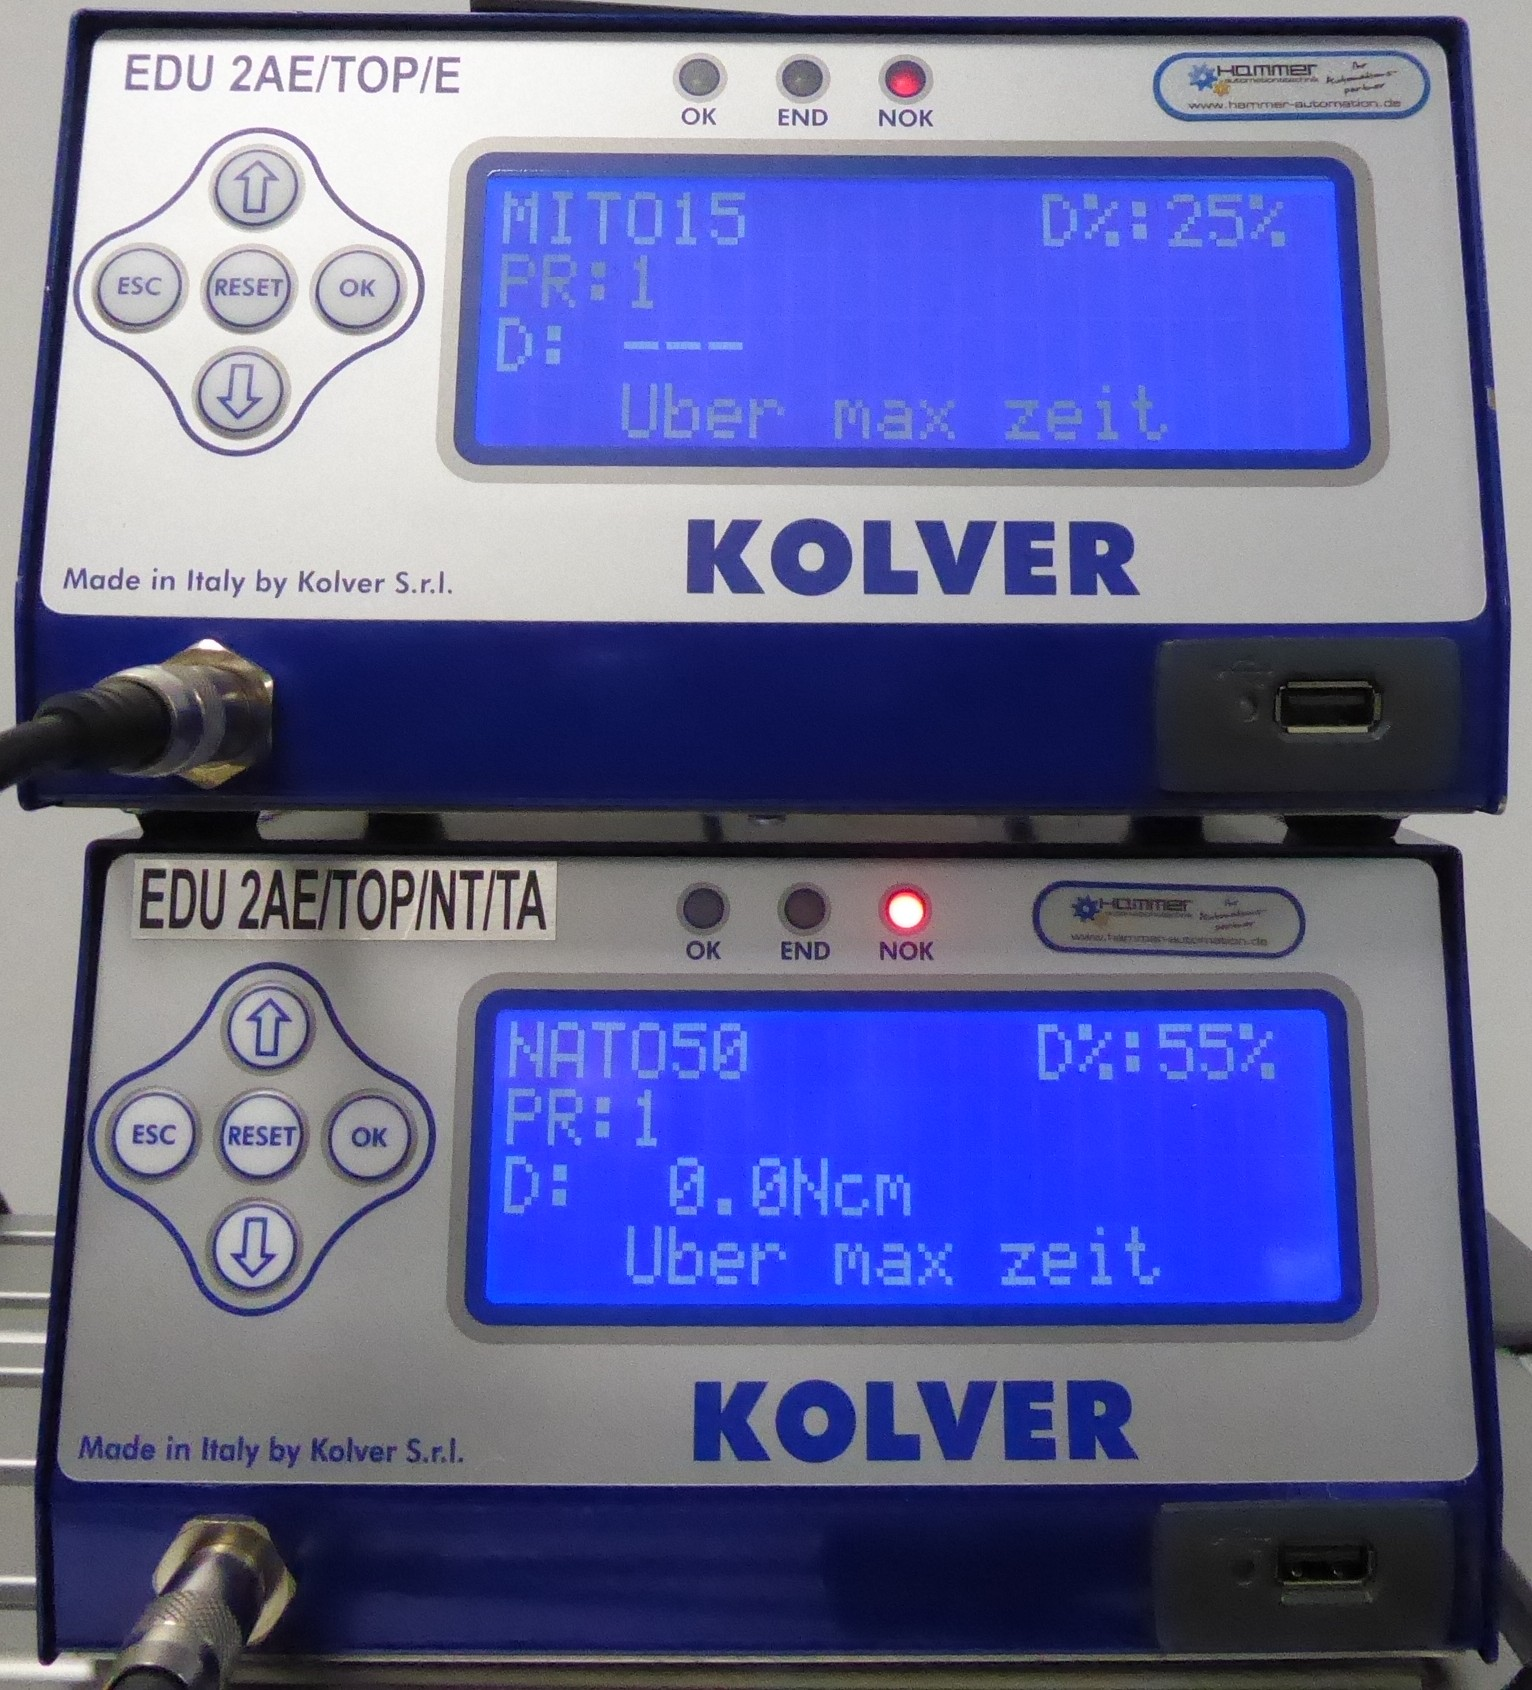
\includegraphics[width=\textwidth]{Bilder/06_Ergebnisse/kolver_nok.JPG}
        \caption{Fehlversuch bei Leerlauftest}
        \label{fig:kolver_nok}
    \end{subfigure}

    \caption{Anzeigezustände der automatischen Schraubendreher auf der EDU-Anzeige während der Tests}
    \label{fig:kolver_zustaende}
\end{figure}

\subsection{Messergebnisse und Beobachtungen}
Die Validierungstests zeigen, dass alle getesteten Aktoren und Sensoren wie vorgesehen funktionieren. Die Positioniergenauigkeit der Linearachsen liegt innerhalb der definierten Toleranzen, und die Sensorik liefert stabile und nachvollziehbare Messwerte.

Es traten keine grundlegenden Probleme auf. Einzelne Auffälligkeiten sind auf den vereinfachten Testaufbau und den Prototypenstatus des Systems zurückzuführen. Für eine abschließende Bewertung wären weiterführende Tests im vollständig integrierten Aufbau erforderlich.

Insgesamt bestätigen die Ergebnisse die grundsätzliche Eignung des entwickelten Systems für den vorgesehenen Montageprozess.\cite{man_trinamic_tmcm6110,man_wago_750system,ds_microepsilon_optoncdt1220}

\clearpage
\section{Fazit und Ausblick}

\subsection{Fazit}
Ziel dieser Arbeit war die Entwicklung eines automatisierbaren Montagekonzepts zum Montieren und Vorspannen von SLC-Linearführungen unter kontrollierten Kraft-, Positions- und Drehmomentbedingungen. Gleichzeitig sollte das System variantenfähig ausgelegt sein und eine Prozessüberwachung der wesentlichen Montageparameter ermöglichen. Dieses Ziel wurde im Rahmen der Arbeit vollständig erreicht.

Das entwickelte Montagesystem ermöglicht das reproduzierbare Vorspannen der Linearführungen sowie die kontrollierte Durchführung der relevanten Montageprozesse. Alle eingesetzten Aktoren und Sensoren funktionieren wie vorgesehen und konnten im Rahmen von Einzeltests erfolgreich in Betrieb genommen werden. Die durchgeführten Validierungstests zeigen, dass die Positioniergenauigkeit sowie die Wiederholbarkeit der Achssysteme innerhalb der geforderten Toleranzen liegen. Auch die Mess- und Überwachungseinrichtungen für Kraft, Position und Drehmoment arbeiten zuverlässig und liefern konsistente Ergebnisse.

Die Variantenfähigkeit des Systems wurde durch die modulare mechanische Auslegung sowie die Verwendung bestehender Werkstückträger sichergestellt. Dadurch können unterschiedliche Baugrößen der SLC-Positionierer ohne grundlegende Anpassungen am System montiert werden. Die Prozessüberwachung ist grundsätzlich realisiert, da alle relevanten Sensoren und Aktoren angebunden und auslesbar sind.

Einschränkend ist festzuhalten, dass der Betrieb des Systems aktuell ausschließlich manuell erfolgt. Ein vollautomatisierter Ablauf wurde im Rahmen dieser Arbeit nicht umgesetzt. Dies ist insbesondere auf die begrenzte verfügbare Bearbeitungszeit zurückzuführen. Dennoch bildet das entwickelte System eine funktionsfähige und validierte Grundlage für eine weiterführende Automatisierung.

\subsection{Ausblick}
Aufbauend auf den Ergebnissen dieser Arbeit ergeben sich mehrere sinnvolle Erweiterungen und Optimierungsmöglichkeiten, um das Montagesystem in Richtung eines industriell einsetzbaren Gesamtsystems weiterzuentwickeln.

Ein wesentlicher nächster Schritt ist die Ausarbeitung und Umsetzung eines vollständigen Sicherheitskonzepts. Die Sicherheit wurde im Rahmen dieser Arbeit bewusst nicht betrachtet. Für einen späteren produktiven Einsatz wären unter anderem ein Not-Aus-Konzept, eine mechanische Einhausung des Systems sowie die Berücksichtigung relevanter allgemeiner Sicherheitsnormen erforderlich.

Des Weiteren sollte die elektrische Integration der Komponenten in einem Schaltschrank erfolgen. Zwar sind alle Komponenten bereits vollständig verdrahtet und funktionsfähig, aktuell befinden sich diese jedoch noch auf dem Arbeitstisch. Ein Schaltschrank würde eine strukturierte, sichere und wartungsfreundliche Unterbringung der Steuerungs- und Leistungskomponenten ermöglichen. Dies ist aus sicherheitstechnischen Gründen erforderlich, insbesondere wenn der Aufbau den Experimentalstatus verlassen und in einen dauerhaften oder erweiterten Betrieb überführt werden soll. Ein entsprechender Schaltplan wurde bereits erstellt und kann hierfür als Grundlage dienen.

\begin{figure}[H]
    \centering
    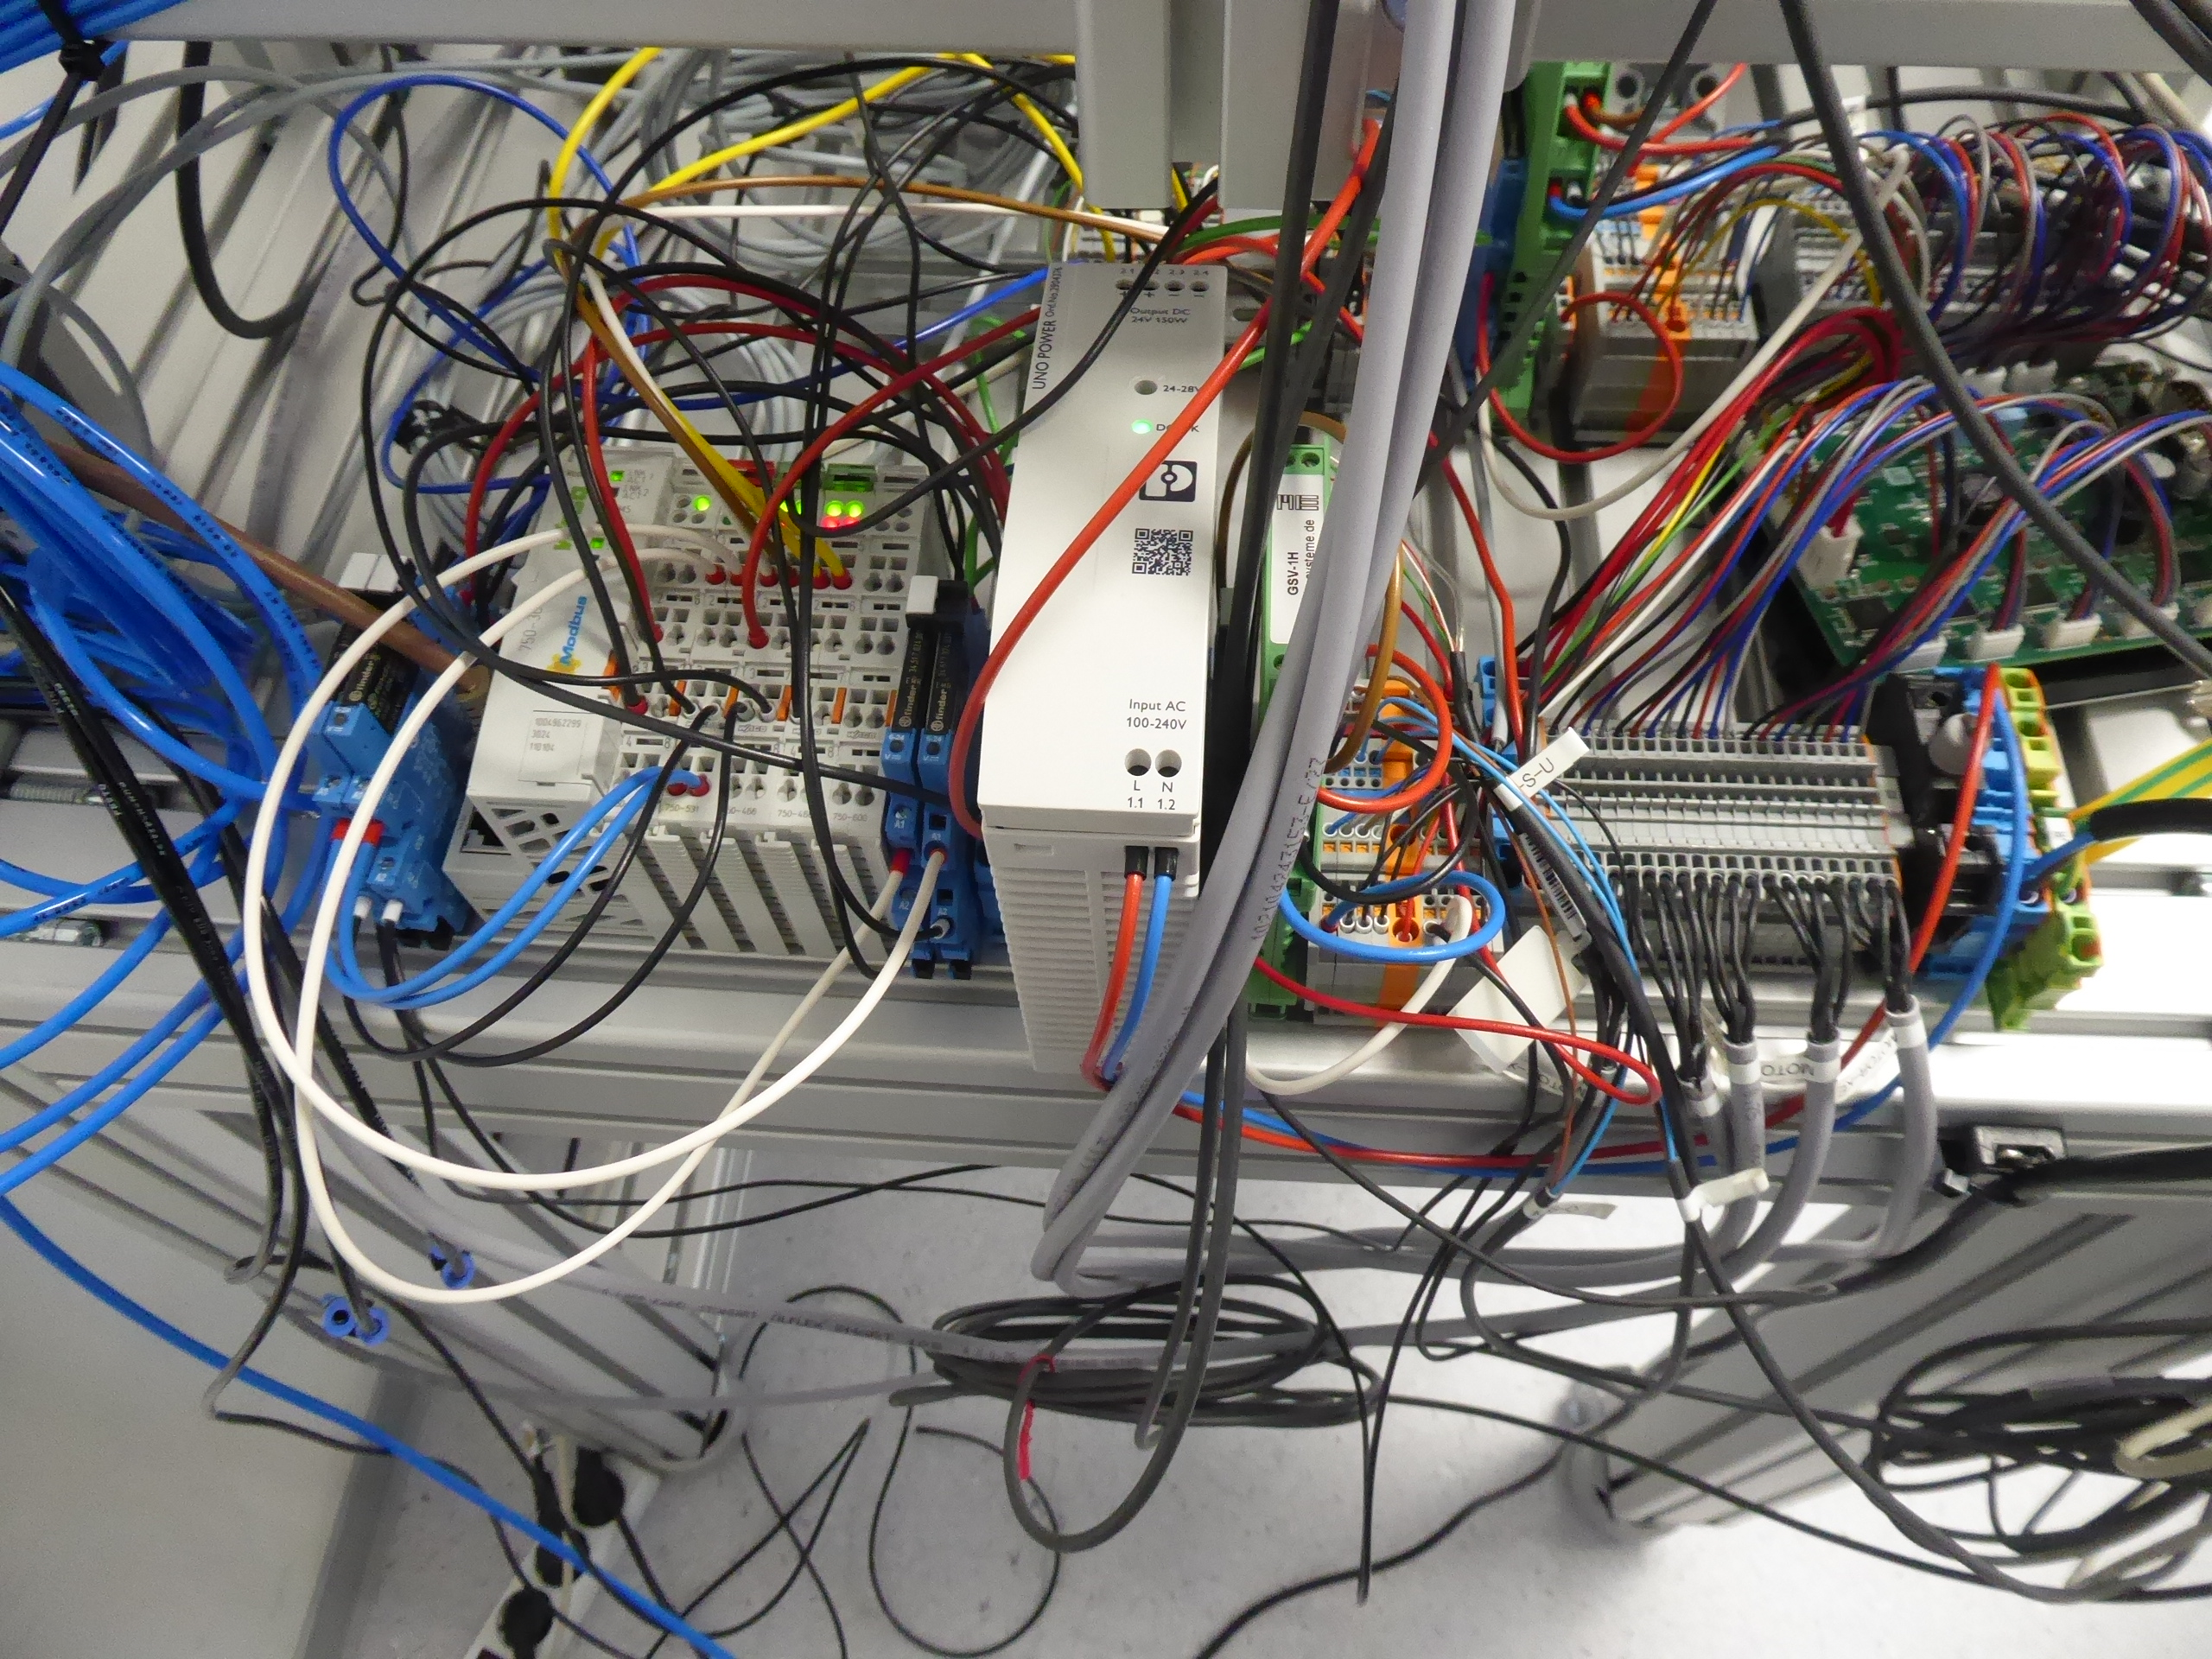
\includegraphics[width=0.5\textwidth]{Bilder/07_Fazit_und_Ausblick/Schaltschrank.JPG}
    \caption{Elektrische Komponenten außerhalb eines Schaltschranks}
\end{figure}

Ein weiterer zentraler Entwicklungsschritt betrifft die Software. Derzeit existieren lediglich Einzeltests ohne durchgängigen Automatisierungscode. Für den automatischen Betrieb wäre die Implementierung eines vollständigen Positionier- und Ablaufprogramms erforderlich. Dieses könnte beispielsweise auf einem PC-basierten System umgesetzt und über Python realisiert werden. Dabei müssten unter anderem Referenzfahrten, Bewegungsprofile, Zustandslogik sowie eine einfache Fehlerbehandlung implementiert werden.

Zusätzlich sollte die Kabelführung des Systems überarbeitet werden. Aktuell ist diese nur provisorisch ausgeführt. Für einen zuverlässigen Dauerbetrieb wären strukturierte Kabelführungen, beispielsweise in Form von Energieketten, sowie geeignete Zugentlastungen notwendig.

\begin{figure}[H]
    \centering
    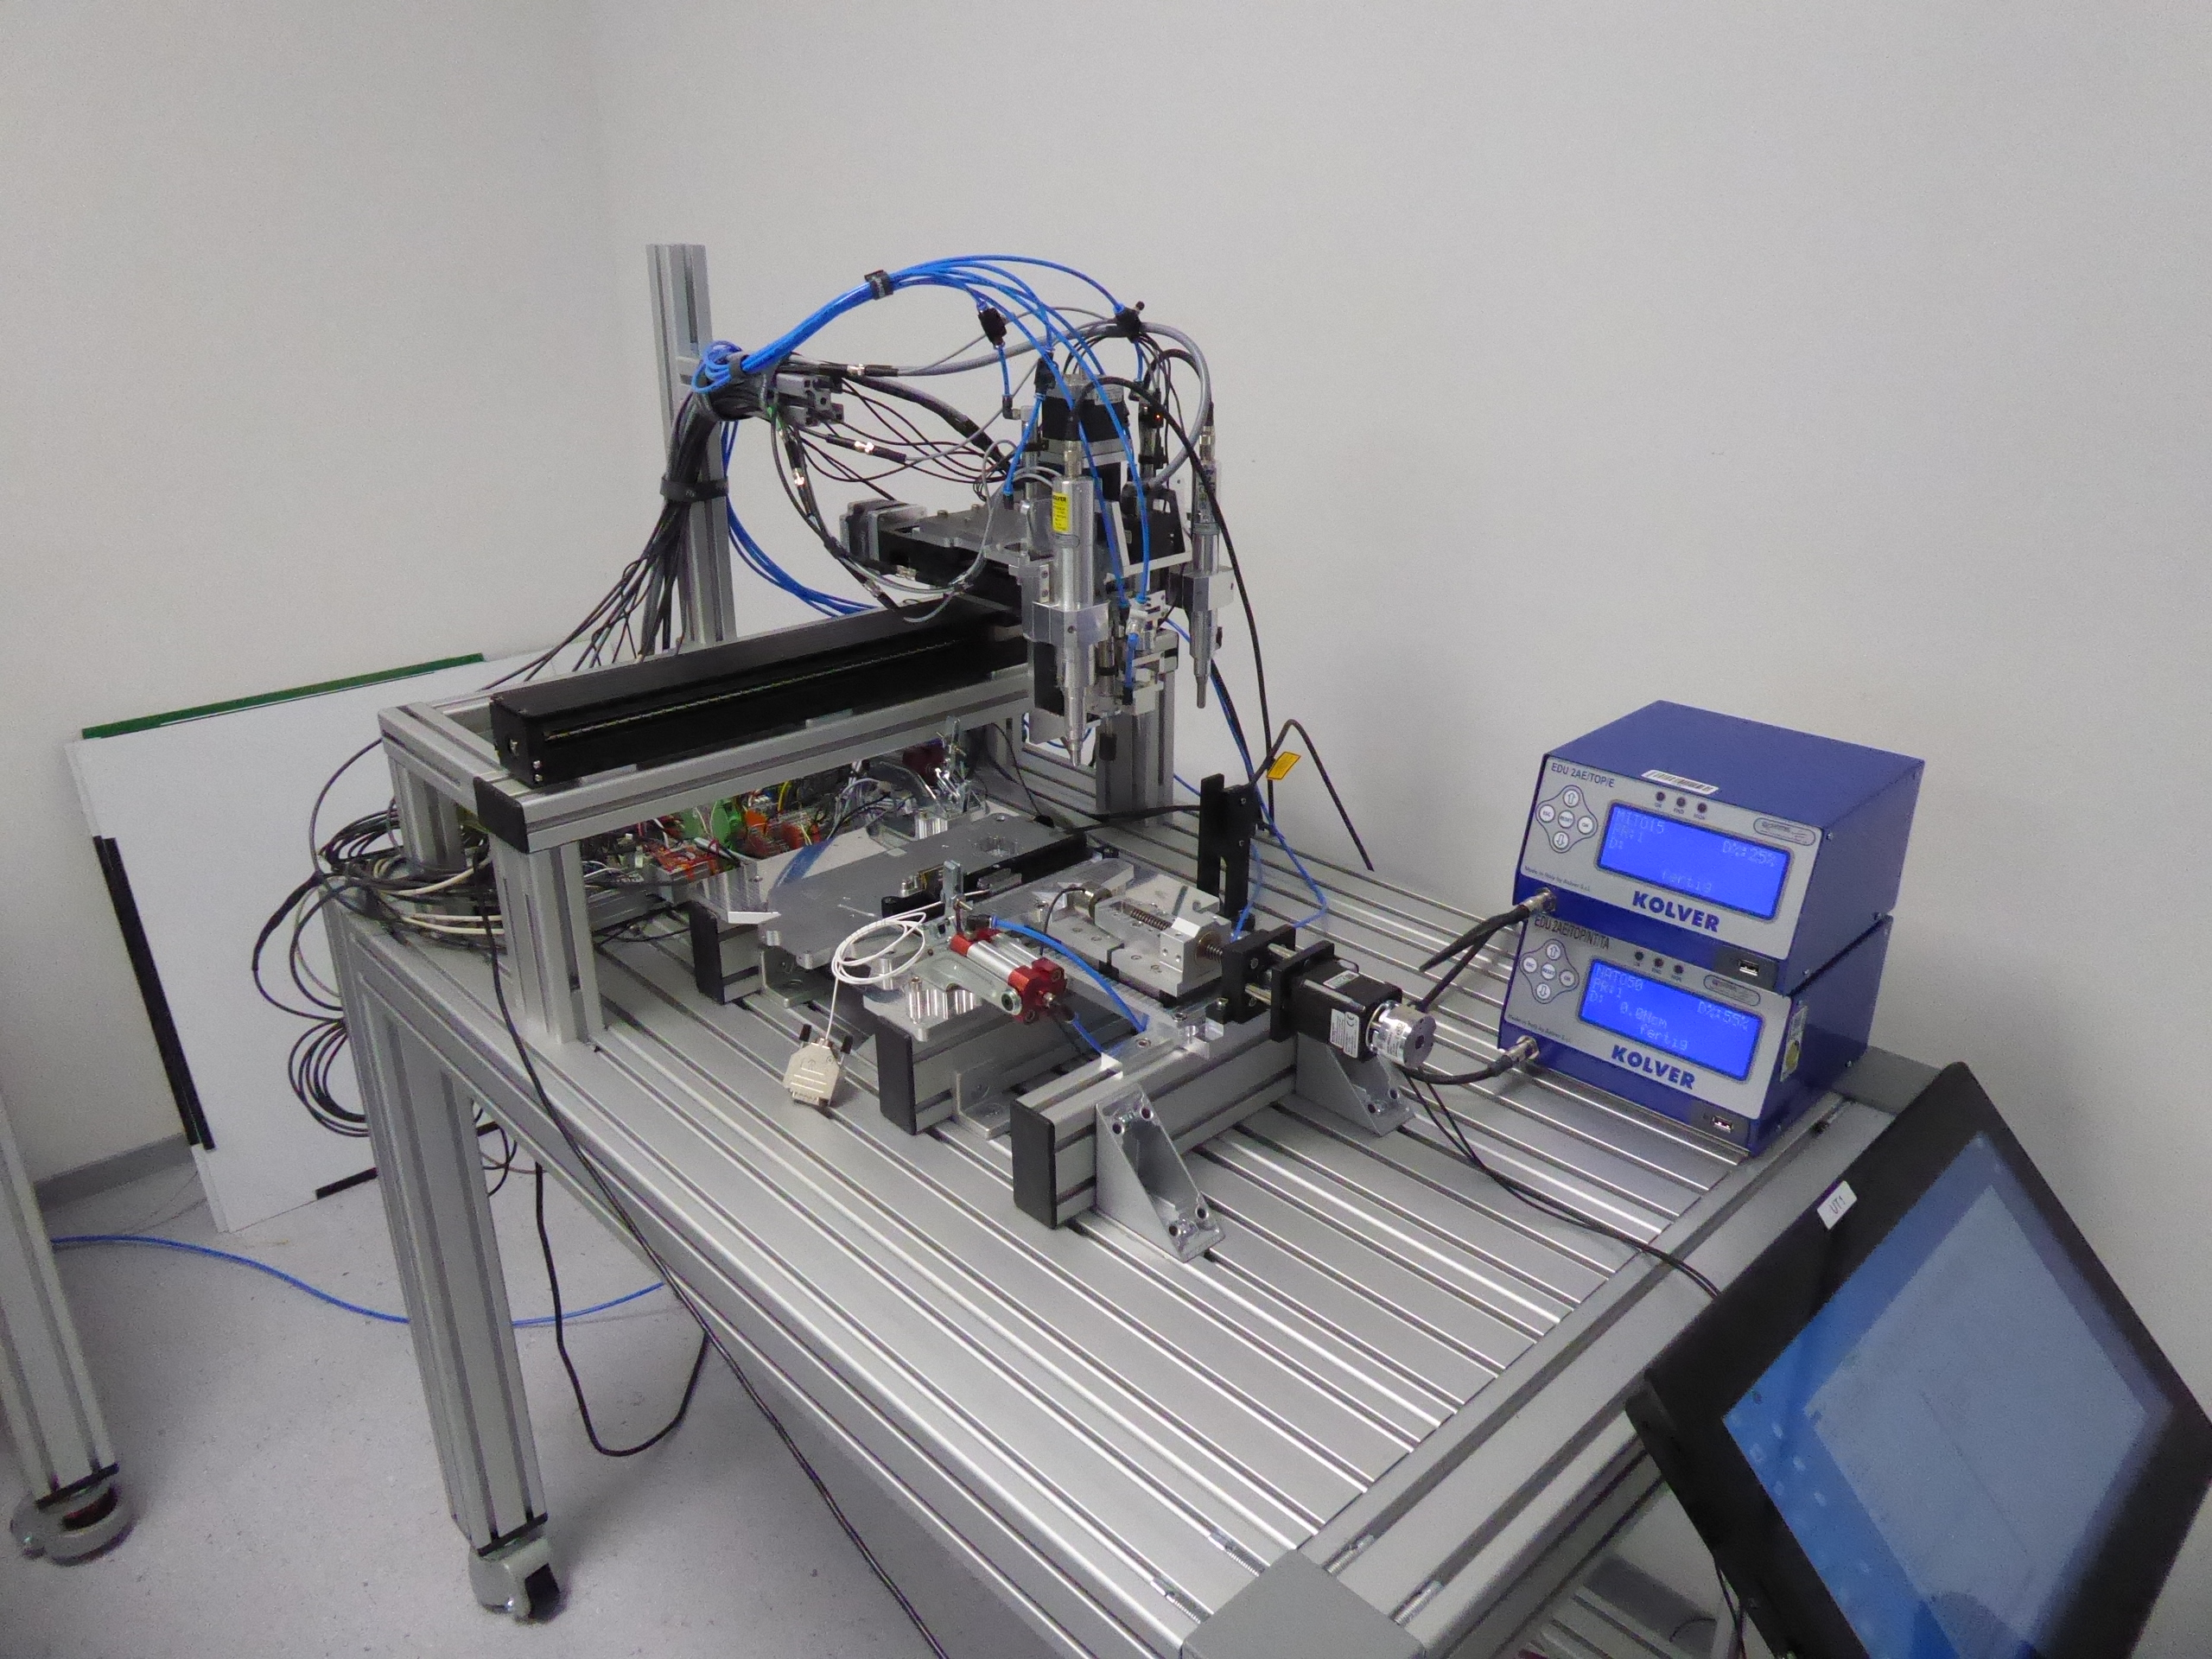
\includegraphics[width=0.5\textwidth]{Bilder/07_Fazit_und_Ausblick/kabelführung.JPG}
    \caption{Provisorische Kabelführung des Versuchsaufbaus}
\end{figure}

Insgesamt stellt das im Rahmen dieser Arbeit entwickelte Montagesystem eine stabile und funktionale Basis dar, auf der zukünftige Erweiterungen in Richtung Automatisierung, Sicherheit und Serienreife systematisch aufbauen können.
\clearpage
\section{Zusammenfassung}
Ziel dieser Arbeit war die Entwicklung eines automatisierbaren Montagekonzepts für SLC-Linearführungen, bei dem das Montieren und Vorspannen der Linearführung unter kontrollierten Kraft-, Positions- und Drehmomentbedingungen erfolgt. Ein besonderer Schwerpunkt lag auf der reproduzierbaren Einstellung der Vorspannung, da diese einen wesentlichen Einfluss auf die Steifigkeit, die Positioniergenauigkeit sowie das Bewegungsverhalten der Positionierer besitzt. Darüber hinaus sollte das Montagekonzept variantenfähig ausgelegt werden, um unterschiedliche SLC-Baugrößen abbilden zu können und eine spätere Prozessüberwachung sowie Automatisierung zu ermöglichen.

Auf Grundlage einer Anforderungsanalyse wurde ein modular aufgebautes Montagesystem konzipiert. Der Aufbau besteht aus einem kartesischen XYZ-Achssystem zur Positionierung der Funktionseinheiten, integrierten Schraubereinheiten für den kontrollierten Verschraubprozess sowie einer mechanischen Vorspann- und Einpressmechanik. Die verwendeten Linearachsen übernehmen ausschließlich Positionieraufgaben und sind auf eine hohe Wiederholgenauigkeit ausgelegt. Der Schraubprozess ist so ausgeführt, dass definierte Drehmomente reproduzierbar aufgebracht werden können. Durch den modularen und klar strukturierten Systemaufbau ist das Montagekonzept grundsätzlich für eine schrittweise Erhöhung des Automatisierungsgrads sowie für eine spätere Integration in industrielle Fertigungsumgebungen geeignet.

Zur Überprüfung der Funktionalität und der Einhaltung der Anforderungen wurden umfangreiche Validierungstests durchgeführt. Die Validierung erfolgte manuell in Form von Einzeltests aller relevanten Aktoren, Sensoren und Schraubereinheiten. Hierzu wurden Referenzfahrten der Achssysteme durchgeführt, Endlagen angefahren sowie wiederholte Positionierbewegungen zwischen definierten Positionen ausgeführt. Die Positioniergenauigkeit wurde mithilfe geeigneter Messmittel überprüft. Die Ergebnisse zeigen eine hinreichend höhe Wiederholgenauigkeit der Achssysteme mit einer Abweichung von 4 bis \qty{8}{\micro\meter} pro Achse. Sämtliche eingesetzten Sensoren lieferten zuverlässige Signalrückmeldungen, und alle Aktoren sowie Schraubereinheiten funktionierten innerhalb der vorgesehenen Betriebsgrenzen. Die durchgeführten Tests bestätigen die grundsätzliche Funktionsfähigkeit und Praxistauglichkeit des entwickelten Montagekonzepts.

Aufgrund des zeitlich begrenzten Rahmens der Bachelorarbeit wurde auf die vollständige Umsetzung einer softwareseitigen Automatisierung verzichtet. Insbesondere die Programmierung der Steuerungslogik, die strukturierte Kabelführung, der Aufbau eines vollständigen Schaltschrankkonzepts sowie die sicherheitstechnische Auslegung des Gesamtsystems konnten nicht abschließend realisiert werden. Diese Punkte wurden bewusst als Abgrenzung der Arbeit definiert und stellen Ansatzpunkte für weiterführende Arbeiten dar.

Als Ausblick bietet sich die vollständige Automatisierung des Montageprozesses durch die Implementierung der Steuerungssoftware an. Ergänzend sollen sicherheitstechnische Aspekte gemäß geltender Normen umgesetzt, eine kontinuierliche Prozessdatenerfassung zur Qualitätsüberwachung integriert sowie das System in eine bestehende Produktionsumgebung eingebunden werden. Das entwickelte Montagekonzept stellt somit eine belastbare Grundlage für die weitere Automatisierung des Aufbaus von SLC-Linearführungen dar.

\clearpage
\printbibliography[heading=bibintoc, title={Literaturverzeichnis}]

\appendix
\section*{Anhang}
\appendixtoc
\captionsetup{listof=false}
\clearpage

\begin{landscape}
\section{Anforderungen}
\subsection{Vollständige Anforderungsliste}

\small
\setlength{\tabcolsep}{3pt}
\renewcommand{\arraystretch}{1.15}
\setlength{\LTcapwidth}{\textwidth}
\captionsetup{justification=raggedright,singlelinecheck=false}

\begin{longtable}{|l|p{2,2cm}|p{8.5cm}|l|l|l|l|l|p{4.0cm}|}

\hline
\textbf{ID} &
\textbf{Kategorie} &
\textbf{Anforderung} &
\textbf{Wert} &
\textbf{Einheit} &
\textbf{Priorität} &
\textbf{Datum} &
\textbf{Status} &
\textbf{Kommentar} \\
\hline
\endfirsthead

\hline
\textbf{ID} &
\textbf{Kategorie} &
\textbf{Anforderung} &
\textbf{Wert} &
\textbf{Einheit} &
\textbf{Priorität} &
\textbf{Datum} &
\textbf{Status} &
\textbf{Kommentar} \\
\hline
\endhead
\endlastfoot

A01 & Funktional &
Das System muss mit den vorhandenen Werkstückträgern (WST) kompatibel sein &
— & — & MUSS & 27.06.25 & Erfüllt &
Ermöglicht automatische Bestückung \\
\hline

A02 & Funktional &
Das System muss die Baugrößen SLC-17 und SLC-24 verarbeiten können &
— & — & MUSS & 27.06.25 & Erfüllt &
SLC-17 = SLC mit 17\,mm Breite \\
\hline

A03 & Funktional &
SLC-Positionierer mit Wand (SLC-W) müssen mittels Keile vorgespannt werden können &
— & — & MUSS & 27.06.25 & Erfüllt &
SLC-W = SLC mit Wand \\
\hline

A04 & Funktional &
SLC-Positionierer ohne Wand müssen mit dem bestehenden Vorspannsystem vorgespannt werden &
— & — & MUSS & 27.06.25 & Erfüllt &
— \\
\hline

A05 & Funktional &
Das Vorspannsystem muss das Führungspaket parallel zur Referenzfläche ausrichten. &
$< 20$ & $\mu$m & MUSS & 27.06.25 & Erfüllt &
Gleiche Breite überall \\
\hline

A06 & Funktional &
Die Schrauben sind mit einem vordefinierten Drehmoment anzuziehen &
25 - 60 & $Ncm$ & MUSS & 27.06.25 & Erfüllt &
— \\
\hline

A07 & Funktional &
Das Schraubwerkzeug muss präzise positioniert werden können &
— & — & MUSS & 27.06.25 & Erfüllt &
— \\
\hline

A08 & Steuerung &
Geeignete Steuerungshardware und -software sind auszuwählen &
— & — & MUSS & 27.06.25 & Erfüllt &
— \\
\hline

A09 & Steuerung &
Testskripte zur Validierung der Steuerungsabläufe sind zu entwickeln &
— & — & MUSS & 27.06.25 & Erfüllt &
— \\
\hline

A10 & Zeitvorgabe &
Die Bearbeitungsdauer pro Positionierer soll unter 5 Minuten liegen &
$< 5$ & min & SOLL & 02.07.25 & Erfüllt &
— \\
\hline

A11 & Mechanik &
Die maximale Systemgröße darf 1200 × 760\,mm nicht überschreiten &
1200 × 760 & mm & MUSS & 27.06.25 & Erfüllt &
— \\
\hline

A12 & Daten\-management &
Relevante Prozessdaten sollen erfasst und dokumentiert werden &
— & — & SOLL & 27.06.25 & In Arbeit &
z.\,B. Seriennummer, Drehmoment, Kraft, Prozessstatus \\
\hline

A13 & Rahmen\-bedingung &
Das Projektbudget beträgt maximal 10.000\,€ &
10.000 & € & MUSS & 27.06.25 & Erfüllt &
— \\
\hline

A14 & Mechanik &
Toleranzen der Montagekomponenten müssen eingehalten werden &
— & — & MUSS & 27.06.25 & Erfüllt &
— \\
\hline

A16 & Sicherheit &
Die genaue Position der Schlitten ist stets zu überwachen &
— & — & MUSS & 27.06.25 & Erfüllt &
— \\
\hline

A19 & Reinraum\-kompatibilität &
Die Station soll für den Einsatz in ISO-6-Umgebungen gemäß ISO 14644-1 geeignet sein &
— & — & SOLL & 29.07.25 & In Arbeit &
— \\
\hline

A19b & Mechanik &
Komponenten müssen robust gegenüber Vibration, Verschleiß und Belastung ausgelegt sein &
— & — & SOLL & 27.06.25 & Erfüllt &
— \\
\hline

A20 & Wartung &
Das System soll wartungsarm und wartungsfreundlich gestaltet sein &
— & — & SOLL & 27.06.25 & Erfüllt &
— \\
\hline

A21 & Erweiter\-barkeit &
Das System soll für künftige Erweiterungen (z.\,B. neue Baugrößen) ausgelegt sein &
— & — & SOLL & 27.06.25 & Erfüllt &
— \\
\hline

A22 & Flexibilität &
Die Umrüstung zwischen SLC-17 und SLC-24 (mit/ohne Wand) soll schnell und werkzeuglos sein &
— & — & SOLL & 27.06.25 & Erfüllt &
— \\
\hline

A23 & Validierung &
Alle Subsysteme sollen kalibriert werden &
— & — & SOLL & 27.06.25 & In Arbeit &
— \\
\hline

A24 & Energie\-effizienz &
Der Energieverbrauch des Systems soll optimiert sein &
— & — & KANN & 30.06.25 & In Arbeit &
— \\
\hline

A25 & Transport &
Das System soll auf Rollen stehen oder modular zerlegbar sein &
— & — & KANN & 30.06.25 & Erfüllt &
— \\
\hline

A26 & Mechanik &
Die Positionierabweichung des Schraubwerkzeugs
darf in jede Richtung nicht größer als \qty{15}{\micro\meter} sein. &
$< 15$ & $\mu$m & MUSS & 30.06.25 & Erfüllt &
— \\
\hline

\caption{Vollständige Anforderungsliste des automatisierten Montagesystems}
\label{tab:anforderungsliste}
\end{longtable}
\end{landscape}

\clearpage

\section{Mechanische Konstruktion}
\label{anhang:2d_zeichnungen}

Die folgenden PDF-Dokumente enthalten die 2D-Zeichnungen der im Montagesystem
verwendeten Baugruppen. Die Zeichnungen dienen der ergänzenden Darstellung
des mechanischen Aufbaus und der Stücklistenstruktur. Die Zeichnungen sind in der folgenden Reihenfolge:

\begin{enumerate}
    \item Gesamtbau
    \item Achssystem
    \item Endeffektor (EE)
    \item Werkstückaufnahme
\end{enumerate}

\clearpage

\begin{landscape}
\label{anhang:gesamtbau}
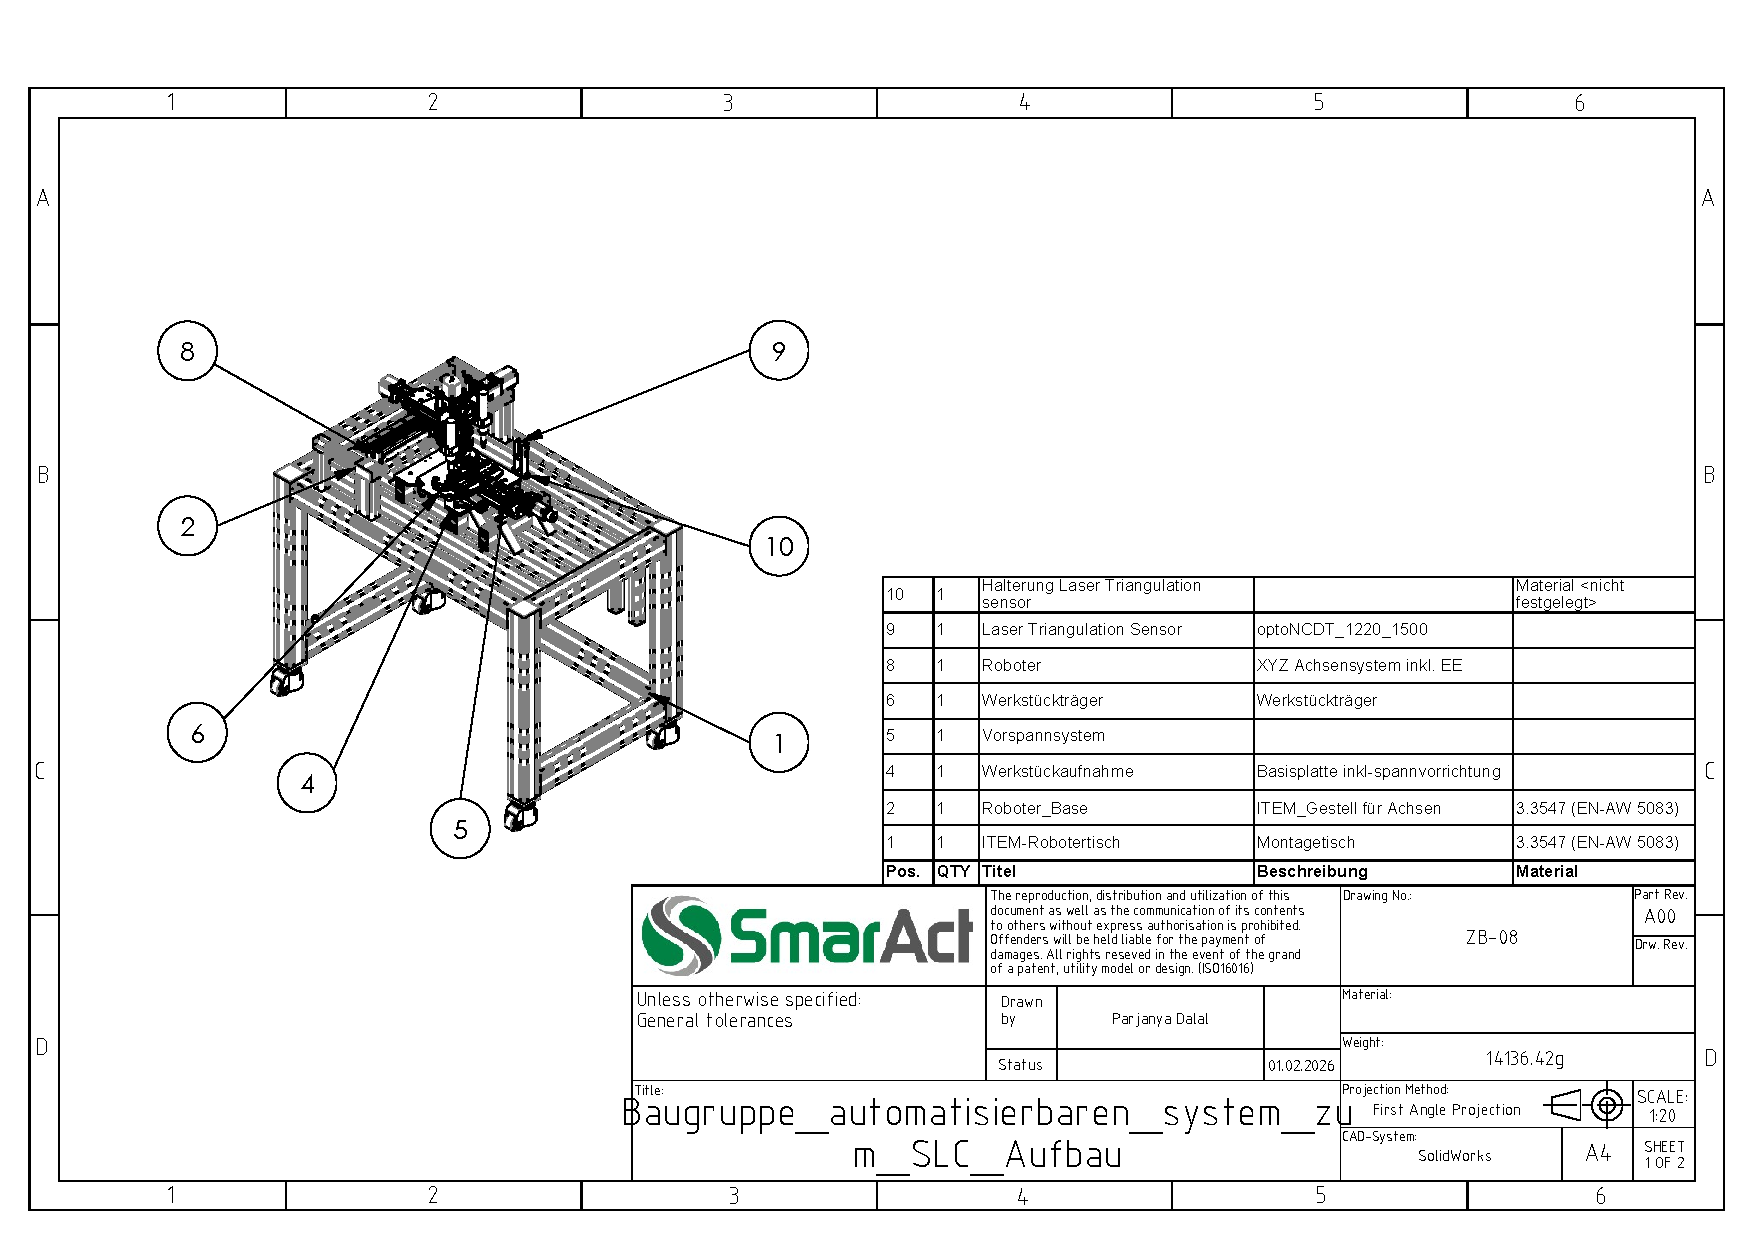
\includepdf[pages={-}, angle=90, scale=0.9]{Anhang/Gesamtbau_pdf.pdf}
\label{anhang:ee_2d}
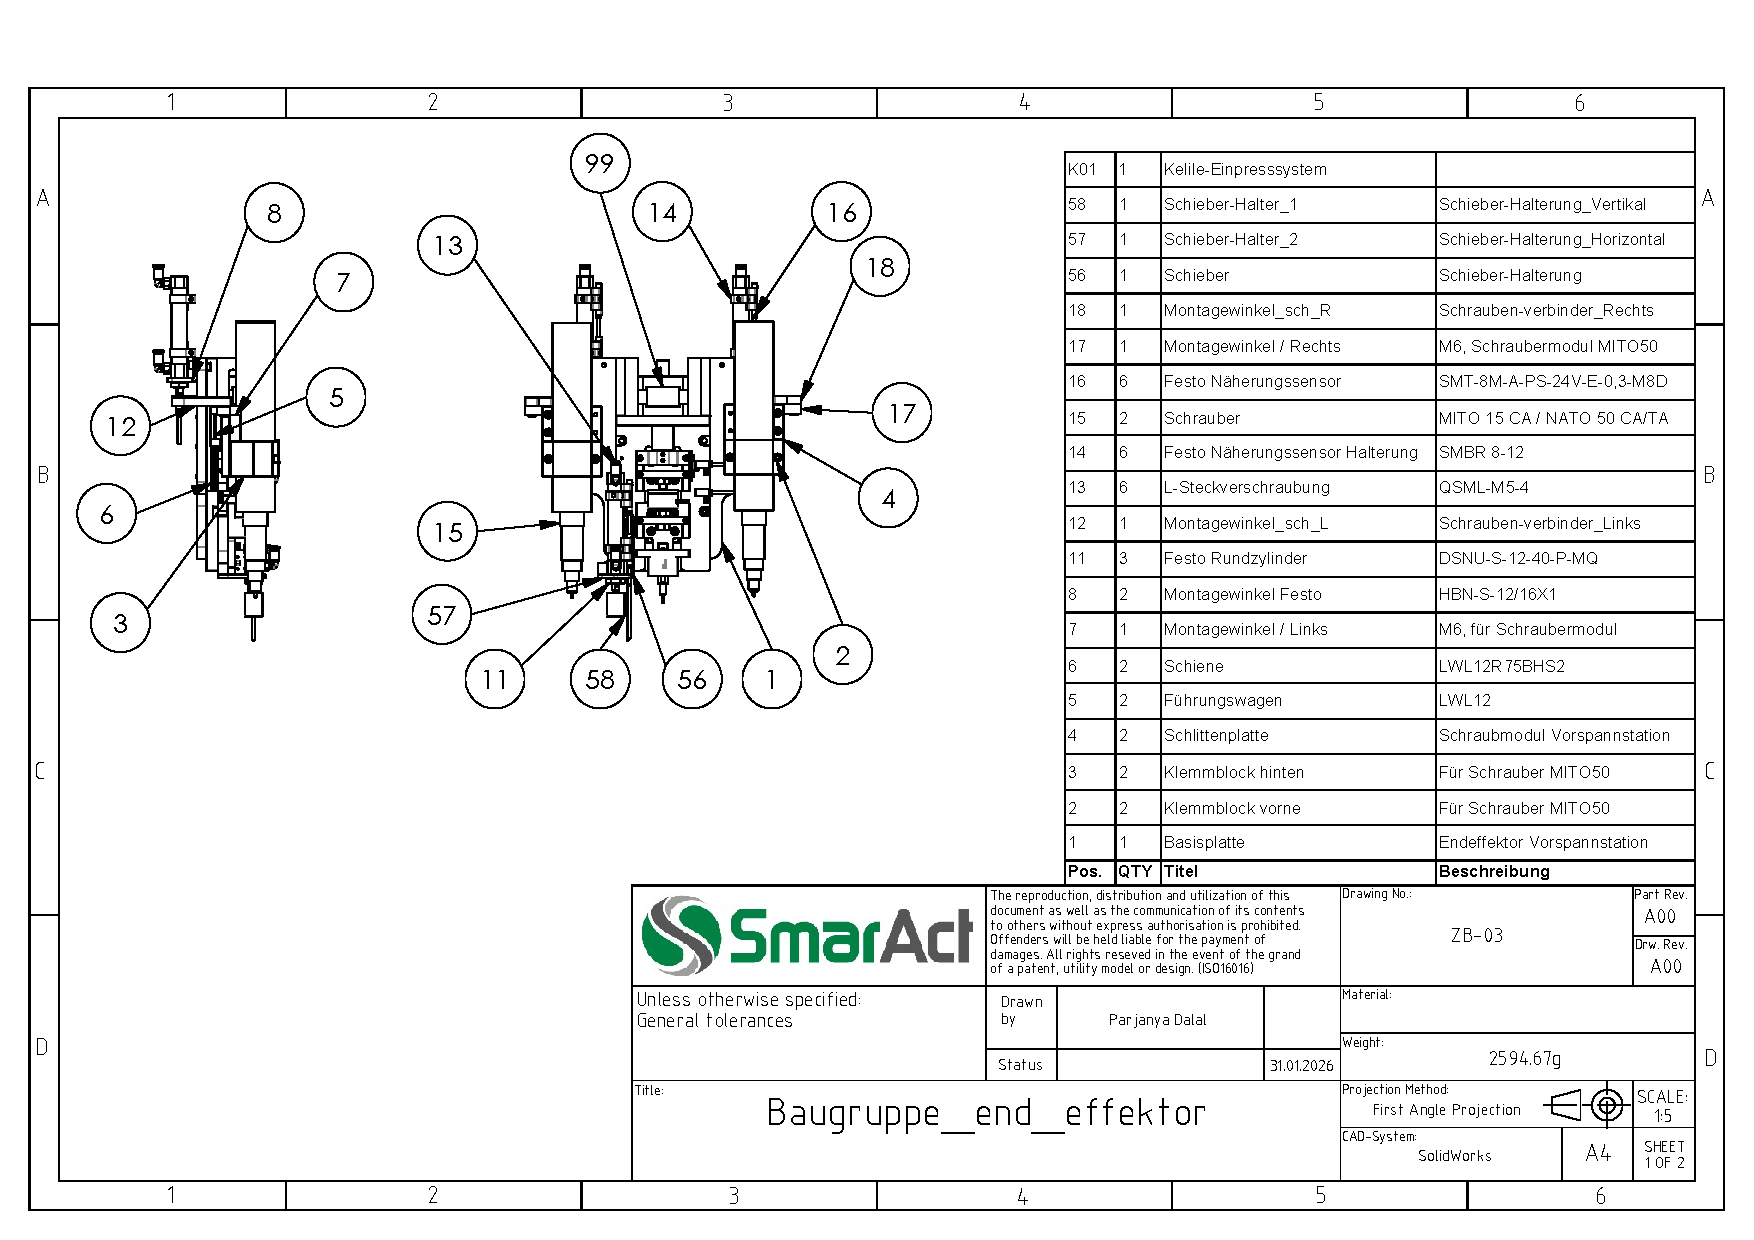
\includepdf[pages={-}, angle=90, scale=0.9]{Anhang/EE_pdf.pdf}
\label{anhang:achssystem}
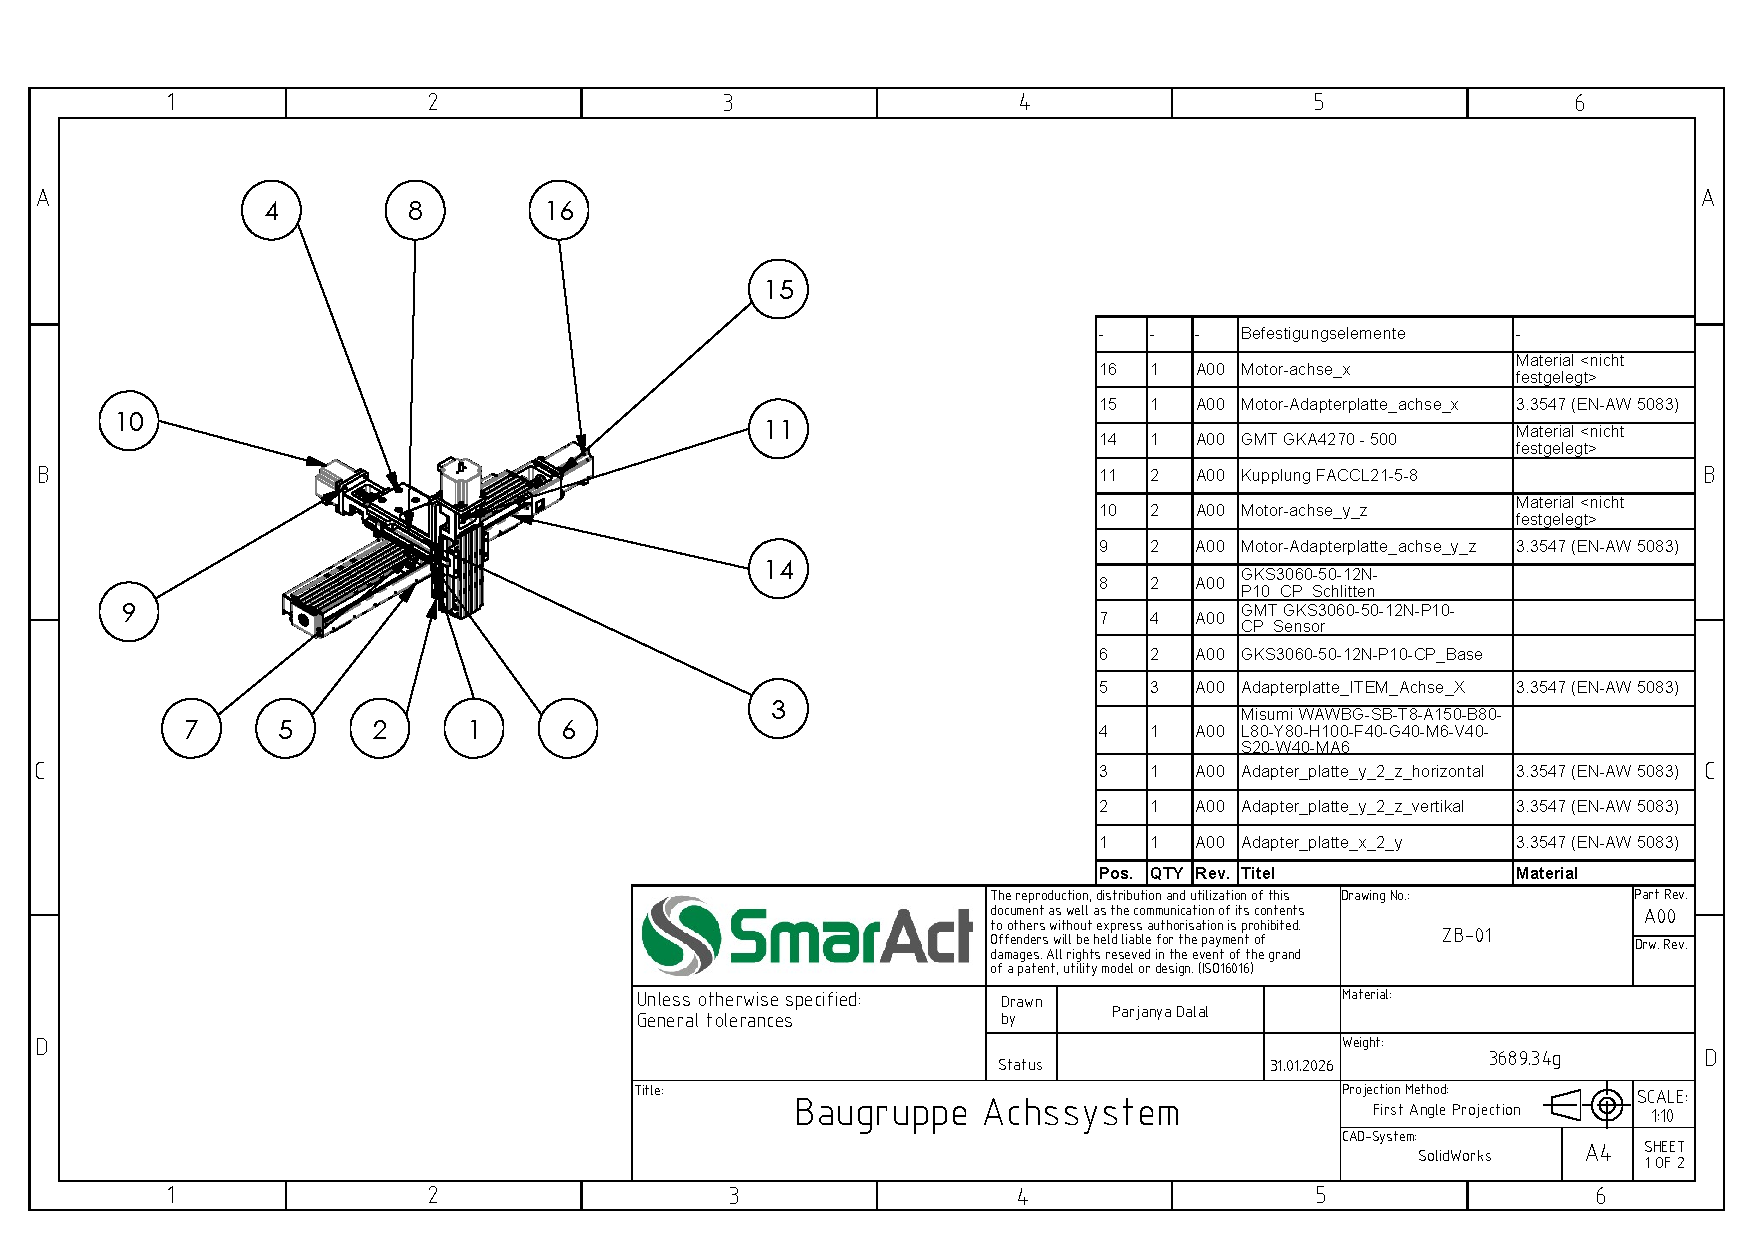
\includepdf[pages=-, angle=90 , scale=0.9]{Anhang/Achssystem_pdf.pdf}
\label{anhang:Werkst.}
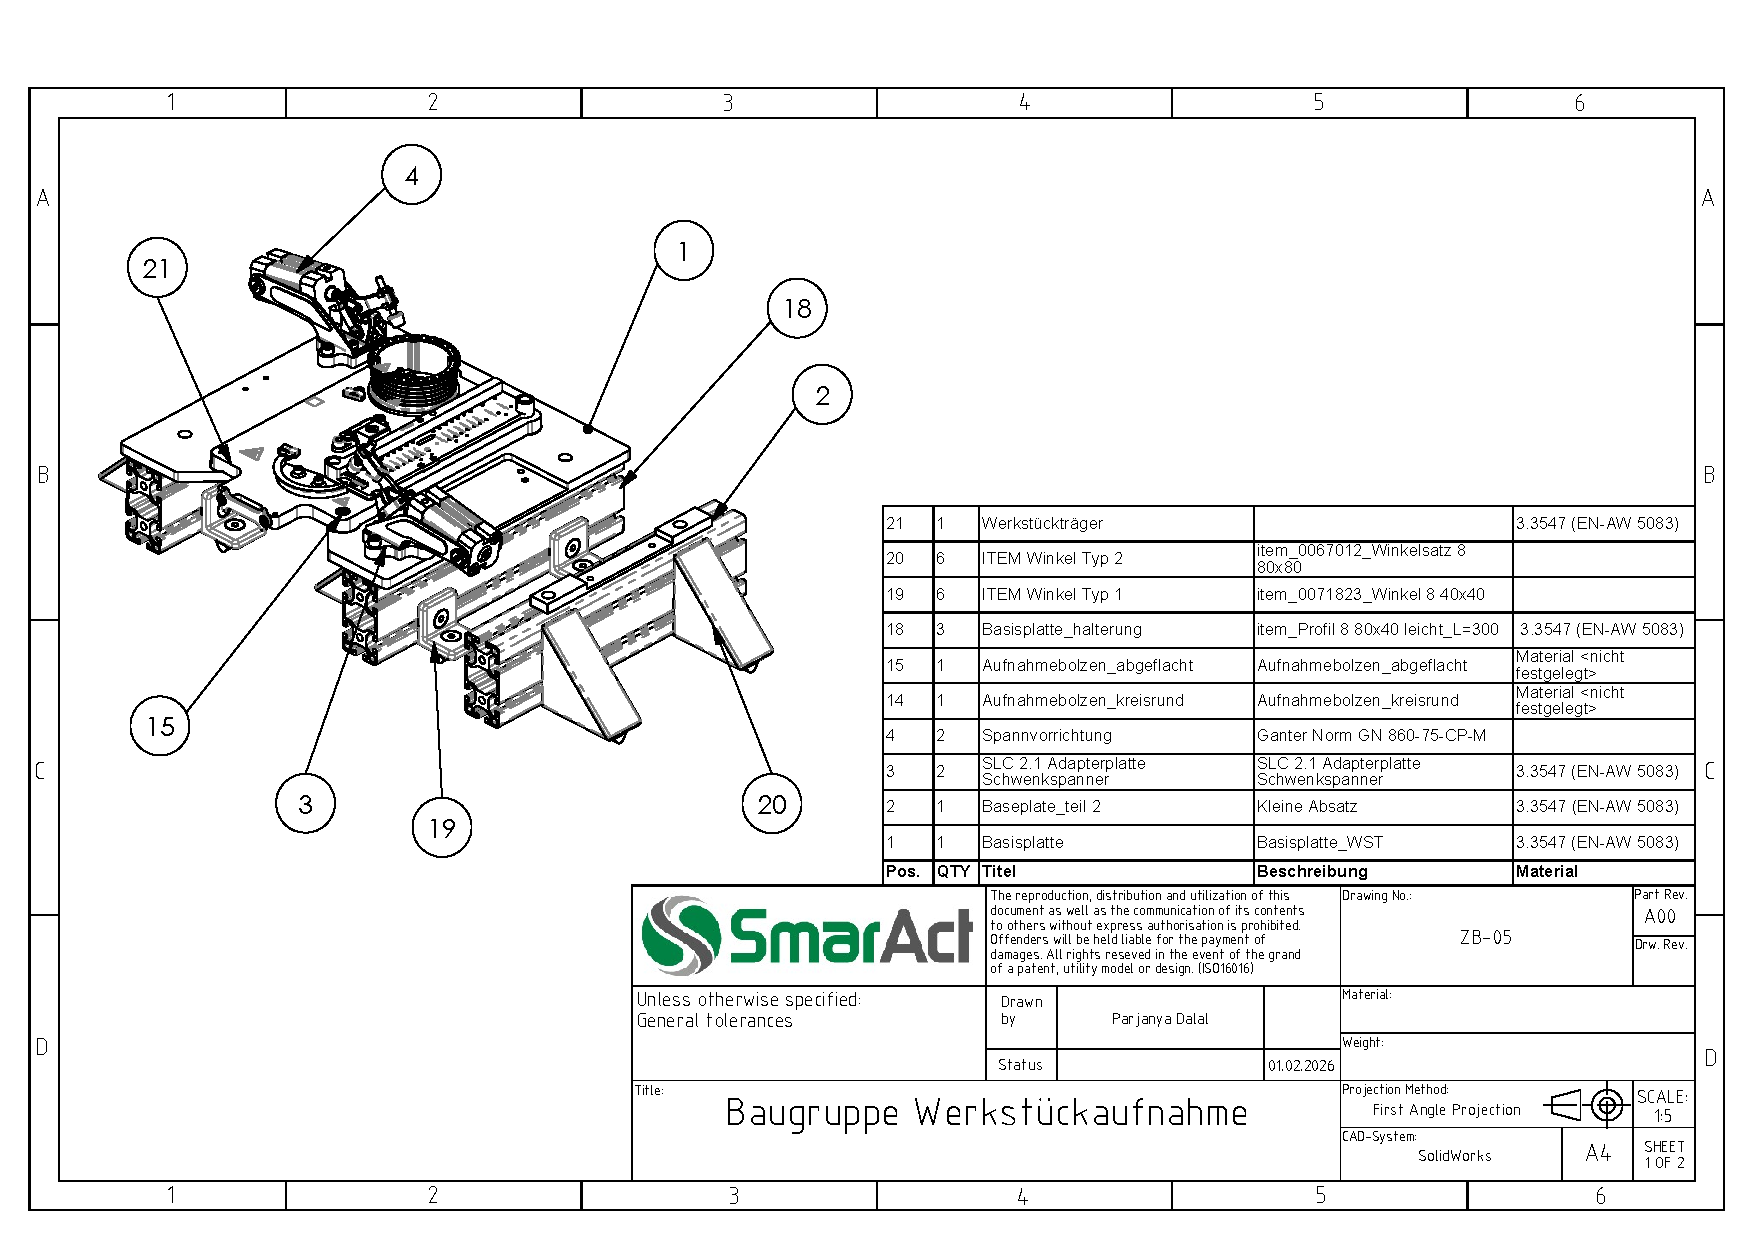
\includepdf[pages={-}, angle=90, scale=0.9]{Anhang/Werkst_pdf_1.pdf}
\end{landscape}
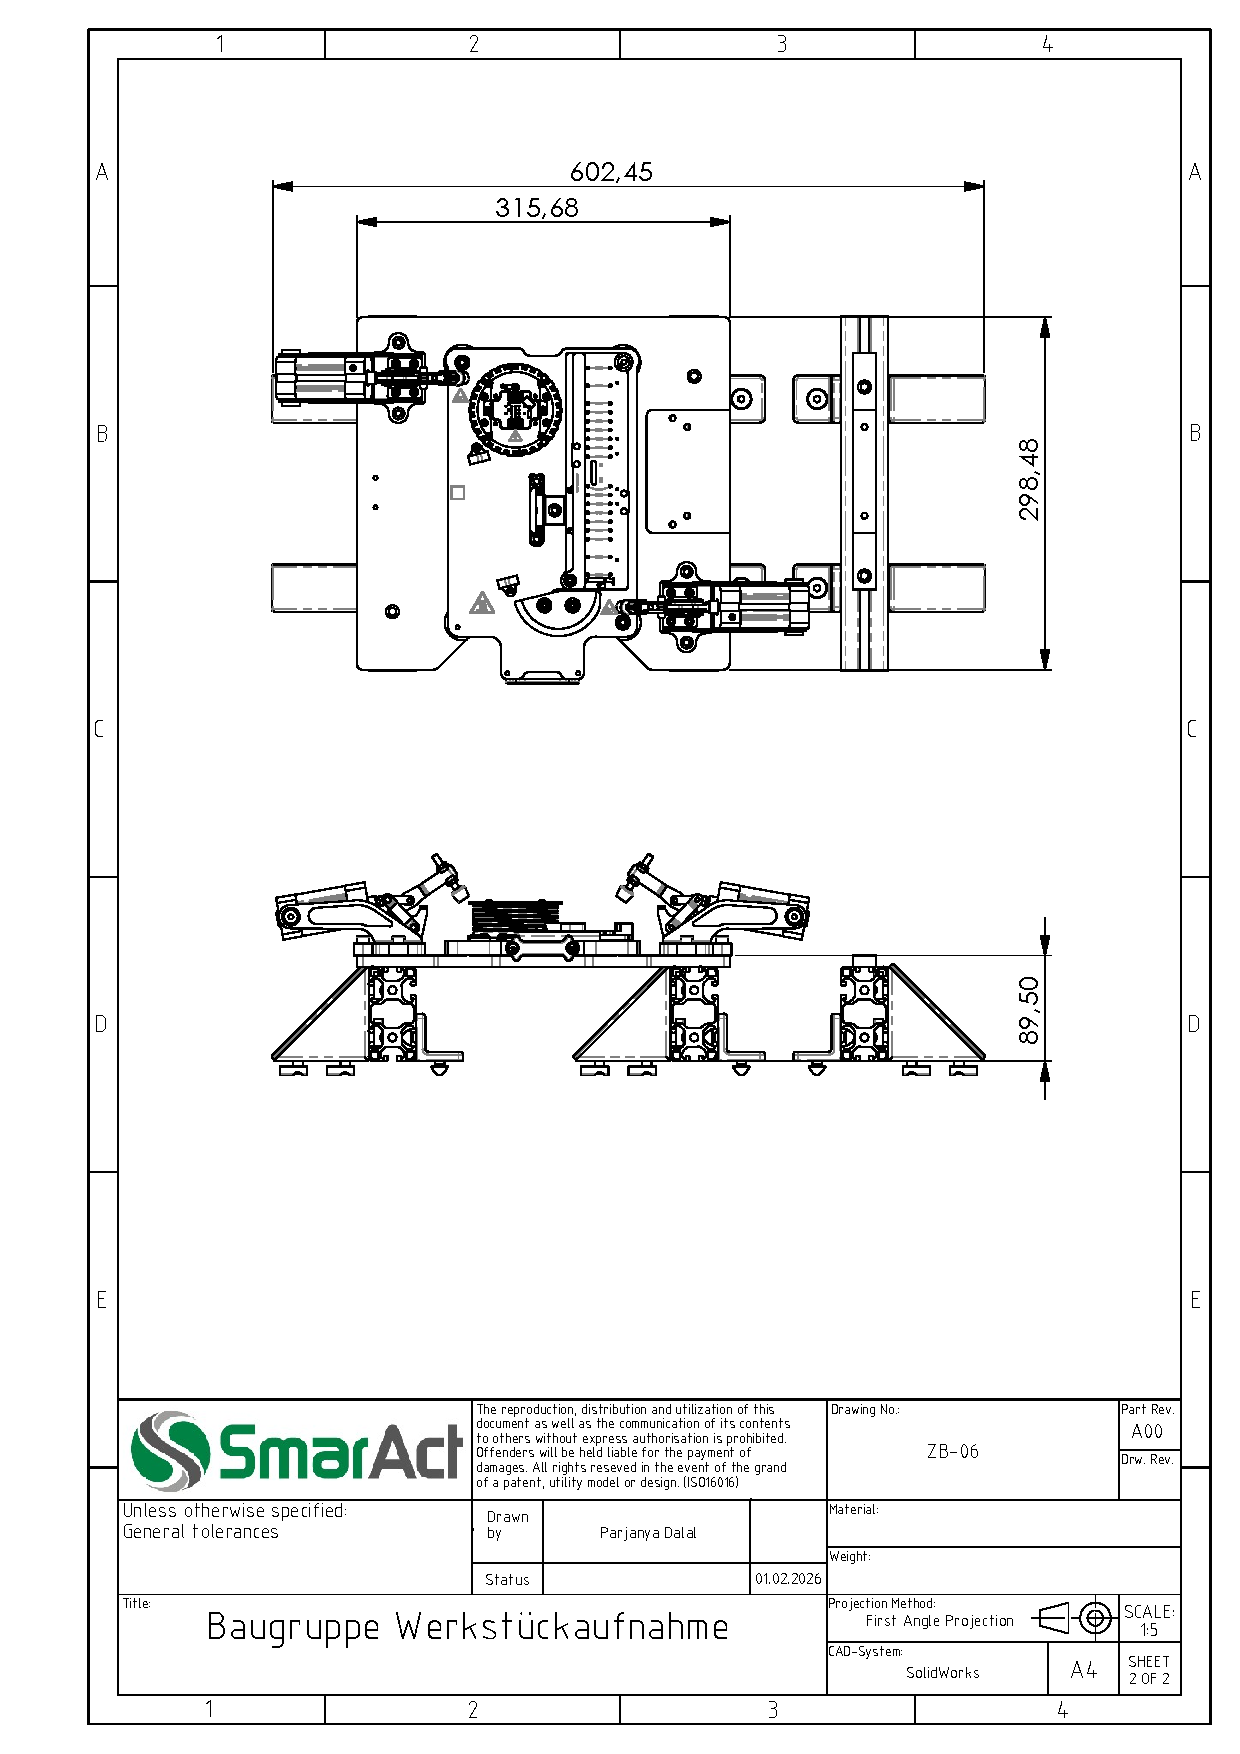
\includepdf[pages={-}, scale=0.9]{Anhang/Werkst_pdf_2.pdf}

\clearpage

\begin{landscape}
\section{Stückliste}
\subsection{Gesamt Stückliste}
{
\small
\setlength{\tabcolsep}{3pt}
\renewcommand{\arraystretch}{1.15}

\begin{longtable}{|l|l|l|l|l|p{4.6cm}|p{6.5cm}|}
\hline
\textbf{Nr.} & \textbf{Menge} & \textbf{Klassifikation} & \textbf{Kategorie} & \textbf{Benennung} & \textbf{Produkt / Typ} & \textbf{Erläuterung} \\
\hline
\endfirsthead

\hline
\textbf{Nr.} & \textbf{Menge} & \textbf{Klassifikation} & \textbf{Kategorie} & \textbf{Benennung} & \textbf{Produkt / Typ} & \textbf{Erläuterung} \\
\hline
\endhead

\endlastfoot

% ---------------- Base ----------------
B01 & 1 & COTS & Base & ITEM Roboter-Tisch & ITEM Profil 8 (Gestell) & Aluminiumprofil-Gestell mit Verbindern, Füßen und Tischplatte \\
\hline
B02 & 1 & COTS & Base & ITEM Roboter-Basis & ITEM Profil 8 (40×40, 40×80) & Aluminiumprofil-Gestell als Basisrahmen \\
\hline
B03 & 3 & COTS & Base & ITEM WST-Basis & ITEM Profil 8 (40×80) & Aluminiumprofil-Gestell zur Aufnahme der WST-Struktur \\
\hline
B04 & 1 & M & Base & WST-Basisplatte Teil 1 & Eigenfertigung (Aluminiumplatte) & Platte zur Aufnahme von WST und Vorspannstation \\
\hline
B05 & 1 & M & Base & WST-Basisplatte Teil 2 & Eigenfertigung (Aluminiumplatte) & Platte zur Aufnahme der Vorspannstation \\
\hline
B06 & 2 & COTS & Base & Passstifte & Passstifte & Fixierung des Werkstückträgers in definierter Position \\
\hline

% ---------------- Keileinpresssystem ----------------
K01 & 1 & M & Keileinpresssystem & Grundplatte & Eigenfertigung & Basisplatte des Keileinpresssystems \\
\hline
K02 & 1 & M & Keileinpresssystem & Motorhalterplatte & Eigenfertigung & Aufnahme des Vertikalantriebs \\
\hline
K03 & 2 & M & Keileinpresssystem & Motorhalter-Halterung & Eigenfertigung & Mechanische Fixierung der Motorhalterplatte \\
\hline
K04 & 1 & M & Keileinpresssystem & M4-Gewindeadapter & Eigenfertigung & Adapterelement zur Montage \\
\hline
K05 & 2 & COTS & Keileinpresssystem & Führungswagen & Misumi SSE2BLZ13G-100 & Linearführungswagen des Keileinpresssystems \\
\hline
K06 & 1 & M & Keileinpresssystem & Einpresskeil & Eigenfertigung & Keil zur Kraftübertragung auf das Führungspaket \\
\hline
K07 & 1 & M & Keileinpresssystem & Federstück & Eigenfertigung & Mechanisches Rückstellelement / Federaufnahme \\
\hline
K08 & 1 & COTS & Keileinpresssystem & Führungsschiene & Misumi SSE2BLZ13G-100 & Linearschiene des Keileinpresssystems \\
\hline
K09 & 1 & COTS & Keileinpresssystem & Kraftmessdose & KM26Z-50N & Kraftsensor zur Prozessüberwachung \\
\hline
K10 & 1 & COTS & Keileinpresssystem & DMS-Verstärker & ME GSV-1H 010/10kHz/2 & Signalaufbereitung der Kraftmessdose \\
\hline
K11 & 1 & COTS & Keileinpresssystem & Schrittmotor (vertikal) & Nanotec LGA421S14-B-UKAS-019 & Vertikalantrieb des Keileinpresssystems \\
\hline
K12 & 2 & COTS & Keileinpresssystem & Gabellichtschranke & Panasonic PM-F25 & Endlagenerfassung des Keilschlittens (2×) \\
\hline
K13 & 2 & COTS & Keileinpresssystem & Druckfeder & 6--10\,mm & Mechanische Vorspannung / Rückstellung \\
\hline
K14 & 1 & M & Keileinpresssystem & Lichtschranken-Pin & 3D-Druck & Betätigungselement für die Gabellichtschranken \\
\hline
K15 & 1 & M & Keileinpresssystem & Schlitten oben & Eigenfertigung & Bewegliches Führungselement (oberes Teil) \\
\hline
K16 & 1 & M & Keileinpresssystem & Schlitten unten & Eigenfertigung & Gegenstück des Schlittens (unteres Teil) \\
\hline
K17 & 1 & COTS & Keileinpresssystem & Universal-Gelenk & GDW1720-W & Mechanische Kraftübertragung / Ausgleich \\
\hline
K18 & 1 & M & Keileinpresssystem & Kraftsensorplatte unten & Eigenfertigung & Adapterplatte zur Integration der Kraftmessdose (unten) \\
\hline
K19 & 1 & M & Keileinpresssystem & Kraftsensorplatte oben & Eigenfertigung & Adapterplatte zur Integration der Kraftmessdose (oben) \\
\hline
K20 & 1 & M & Keileinpresssystem & Flansch & Eigenfertigung & Verbindungselement zum Antrieb / zur Struktur \\
\hline

% ---------------- Robotersystem ----------------
R01 & 1 & COTS & Robotersystem & Linearachse X & GKA4270-500-12N-P10 & Portalachse für horizontale Positionierung (X) \\
\hline
R02 & 1 & COTS & Robotersystem & Linearachse Y & GKS3060-50-12N-P5 & Querachse des Portals (Y) \\
\hline
R03 & 1 & COTS & Robotersystem & Linearachse Z & GKS3060-50-12N-P6 & Vertikalachse des Portals (Z) \\
\hline
R04 & 1 & COTS & Robotersystem & Schrittmotor X & Nanotec SCA5618L4204-B2 (NEMA 23, 3\,Nm) & Antrieb der X-Achse \\
\hline
R05 & 1 & COTS & Robotersystem & Schrittmotor Y & Nanotec SCB6018M4204-B (NEMA 23, 2\,Nm) & Antrieb der Y-Achse \\
\hline
R06 & 1 & COTS & Robotersystem & Schrittmotor Z & Nanotec SCB6018M4204-B (NEMA 23, 2\,Nm) & Antrieb der Z-Achse \\
\hline
R07 & 3 & M & Robotersystem & Adapterplatte ITEM–X & Eigenfertigung & Verbindung X-Achse mit ITEM-Gestell (3×) \\
\hline
R08 & 1 & M & Robotersystem & Adapterplatte X–Y & Eigenfertigung & Verbindung X- zu Y-Achse \\
\hline
R09 & 1 & M & Robotersystem & Adapterplatte Y–Z (1) & Eigenfertigung & Verbindung Y-Achse mit Zwischenplatte \\
\hline
R10 & 1 & M & Robotersystem & Adapterplatte Y–Z (2) & Eigenfertigung & Verbindung Zwischenplatte mit Z-Achse \\
\hline
R11 & 1 & COTS & Robotersystem & Winkelplatte & Misumi (90°-Befestigung) & Montageelement zur 90°-Befestigung \\
\hline

% ---------------- Schraubereinheit ----------------
S01 & 1 & M & Schraubereinheit & Endeffektor-Grundplatte & Eigenfertigung & Verbindung Adapterplatte Y--Z (2) mit Endeffektor \\
\hline
S02 & 2 & COTS & Schraubereinheit & Führungsschiene & LWL 12R75BHS2 & Linearschiene der Schraubereinheit (2×) \\
\hline
S03 & 2 & COTS & Schraubereinheit & Führungswagen & LWL 12 & Lineare Führung des Schraubschlittens (2×) \\
\hline
S04 & 2 & M & Schraubereinheit & Schlittenadapterplatte & Eigenfertigung & Verbindung Schlitten--Werkzeug (2×) \\
\hline
S05 & 2 & M & Schraubereinheit & Klemmblock hinten & Eigenfertigung & Fixierung des Schraubers (hinten, 2×) \\
\hline
S06 & 2 & M & Schraubereinheit & Klemmblock vorne & Eigenfertigung & Fixierung des Schraubers (vorne, 2×) \\
\hline
S07 & 2 & M & Schraubereinheit & Montagewinkel (Festo) & Eigenfertigung / Montagewinkel & Pneumatik-Anbindung der Schraubereinheit \\
\hline
S08 & 3 & COTS & Schraubereinheit & Pneumatikzylinder & Festo DSNU-S-12-40-P-MQ & Zustellbewegung der Schrauber \\
\hline
S09 & 6 & COTS & Schraubereinheit & L-Steckverschraubung & Festo L-Steckverschraubung & Pneumatische Verbindung (6×) \\
\hline
S10 & 6 & COTS & Schraubereinheit & Näherungssensor-Halter & Festo SMBR 8-12 & Halter für Näherungssensoren (6×) \\
\hline
S11 & 6 & COTS & Schraubereinheit & Näherungssensor & Festo SMT-8M-A-PS-24V-E-0,3-M8D & Endlagen-/Positionsabfrage (6×) \\
\hline
S12 & 1 & M & Schraubereinheit & Montagewinkel rechts & Eigenfertigung & Mechanische Verbindung (rechts) \\
\hline
S13 & 1 & M & Schraubereinheit & Montagewinkel links & Eigenfertigung & Mechanische Verbindung (links) \\
\hline
S14 & 1 & M & Schraubereinheit & Verbinder rechts & Eigenfertigung (L-Form) & Verbindung Piston--Schlitten (rechte Seite) \\
\hline
S15 & 1 & M & Schraubereinheit & Verbinder links & Eigenfertigung (L-Form) & Verbindung Piston--Schlitten (linke Seite) \\
\hline
S16 & 1 & COTS & Schraubereinheit & Schrauber SLC24 & MITO15CA & Automatischer Schrauber für SLC-24 \\
\hline
S17 & 1 & COTS & Schraubereinheit & Schrauber SLC17 & NATO50CA/TA & Automatischer Schrauber für SLC-17 \\
\hline

% ---------------- Schieber ----------------
SI01 & 1 & M & Schieber & Halterung vertikal & Eigenfertigung & Halterung Pneumatikzylinder vertikal \\
\hline
SI02 & 1 & M & Schieber & Halterung horizontal & Eigenfertigung & Halterung Pneumatikzylinder horizontal \\
\hline
SI03 & 1 & M & Schieber & Schieber & 3D-Druck & Provisorischer Schieber (3D-gedruckt) \\
\hline

% ---------------- Vorspannsystem ----------------
V01 & 1 & M & Vorspannsystem & Schraubstock & Eigenfertigung / Montage & Vorspannen der SLC-Führung (Einspannung) \\
\hline
V02 & 1 & COTS & Vorspannsystem & Kraftmessdose & KM26Z-500N & Messung der Vorspannkraft \\
\hline
V03 & 1 & COTS & Vorspannsystem & DMS-Verstärker & ME GSV-1H 010/10kHz/2 & Signalaufbereitung der Kraftmessdose \\
\hline
V04 & 1 & M & Vorspannsystem & Druckstange & Eigenfertigung & Verbindung Spindel--Kraftmessdose \\
\hline
V05 & 1 & M & Vorspannsystem & Adapterplatte unten & Eigenfertigung & Adapterplatte: Schlitten zur Schraubstockaufnahme \\
\hline
V06 & 1 & M & Vorspannsystem & Adapterplatte oben & Eigenfertigung & Adapterplatte: Schlitten zur Spindelmutter (Log Nut) \\
\hline
V07 & 2 & COTS & Vorspannsystem & Linearführungsschlitten & MISUMI SSE2BWZ16G-190 & Schlitten des Vorspannsystems (2×) \\
\hline
V08 & 1 & COTS & Vorspannsystem & Linearführungsschiene & NB Guide SERS15WA (Japan SM6722) & Schiene des Vorspannsystems \\
\hline
V09 & 1 & COTS & Vorspannsystem & Trapezgewindemutter & Tr12×3 Log Nut (im Gehäuse) & Spindelmutter im Gehäuse \\
\hline
V10 & 1 & COTS & Vorspannsystem & Trapezgewindespindel & Tr12×3 (gerollt, verlängert) & Linearantrieb der Vorspannmechanik \\
\hline
V11 & 1 & COTS & Vorspannsystem & Festlagergehäuse & dold FLB16-30/8 & Lagerung der Spindel / Adapter \\
\hline
V12 & 1 & COTS & Vorspannsystem & Schrittmotor & Nanotec ST4118D1804-B (NEMA 17, mit Bremse) & Antrieb der Vorspannspindel \\
\hline
V13 & 1 & COTS & Vorspannsystem & Kupplung & dold RB flexibel D18L25 (5{,}00/6{,}00\,mm) & Motor--Spindel-Verbindung \\
\hline
V14 & 1 & M & Vorspannsystem & Grundplatte & Eigenfertigung & Aufnahme / Halterung des Vorspannsystems \\
\hline

% ---------------- Steuerung ----------------
C01 & 1 & COTS & Steuerung & Motorcontroller & TMCM-6110 & Ansteuerung der Schrittmotorachsen \\
\hline
C02 & 4 & COTS & Steuerung & Magnetventil & Festo & Pneumatische Ansteuerung (z.\,B. Zylinder) \\
\hline
C03 & 1 & COTS & Steuerung & Laser-Triangulationssensor & optoNCDT 1220-500 & Positionsmessung des Schlittens \\
\hline
C04 & 1 & COTS & Steuerung & Modbus-Koppler & WAGO 750-362 & Feldbus-Anbindung \\
\hline
C05 & 1 & COTS & Steuerung & Potentialeinspeisung & WAGO 750-602 & 24-VDC-Versorgung / Einspeisung \\
\hline
C06 & 1 & COTS & Steuerung & Digitalausgangsmodul & WAGO 750-531 & Aktoransteuerung (DO) \\
\hline
C07 & 2 & COTS & Steuerung & Analogeingangsmodul & WAGO 750-466 & Sensoranbindung (AI) \\
\hline
C08 & 1 & COTS & Steuerung & Endmodul & WAGO 750-600 & Abschluss der WAGO-Klemme \\
\hline
C09 & 1 & COTS & Steuerung & Netzteil & Phoenix Contact UNO-PS/1AC/24DC/60W & 24-VDC-Stromversorgung \\
\hline
C10 & 6 & COTS & Steuerung & Koppelrelais & Finder 34.51.7.024.0050 & Galvanische Trennung / Relaiskopplung (6×) \\
\hline

\caption{Gesamtstückliste des automatisierten Montagesystems}
\label{tab:gesamt_stueckliste}
\end{longtable}
}
\end{landscape}

\clearpage

\section{Berechnungen}
\label{anhang:berechnungen}
%======================================================================
\subsection{Achssysteme X-, Y- und Z-Achse (eigene Auslegung)}
%======================================================================

\subsubsection{Berechnung der theoretischen Schrittauflösung}

Für alle drei Achsen kommen Schrittmotoren mit einem Schrittwinkel von \SI{1,8}{\degree} zum Einsatz.
Daraus ergeben sich
\begin{equation}
N_\text{Vollschritte}=\frac{360^\circ}{1,8^\circ}=200\ \text{Vollschritte/U}.
\end{equation}

Die Microstep-Auflösung ist über den Achsparameter SAP~140 aus der Trinamic Steuerung eingestellt. In der verwendeten Konfiguration gilt:
\begin{align}
\text{Achse 0 (X):} \quad & \text{SAP 140} = 5 \Rightarrow m_X = 32\ \text{Microsteps/Vollschritt} \\
\text{Achse 1 (Y):} \quad & \text{SAP 140} = 4 \Rightarrow m_Y = 16\ \text{Microsteps/Vollschritt} \\
\text{Achse 2 (Z):} \quad & \text{SAP 140} = 4 \Rightarrow m_Z = 16\ \text{Microsteps/Vollschritt}
\end{align}

Damit ergeben sich die Microsteps pro Umdrehung:
\begin{align}
N_{\mu\text{steps/U},X} &= 200\cdot 32 = 6400,\\
N_{\mu\text{steps/U},Y} &= 200\cdot 16 = 3200,\\
N_{\mu\text{steps/U},Z} &= 200\cdot 16 = 3200.
\end{align}

Die Spindelsteigungen ergeben sich aus den verwendeten Achstypen:
\begin{align}
\text{X-Achse:} \quad & \text{GKA4270-500-12N-P10} \Rightarrow p_X=\SI{10}{mm/U}
 \\
\text{Y-/Z-Achse:} \quad & \text{GKS3060-50-12N-P5} \Rightarrow p_Y=p_Z=\SI{5}{mm/U}
\end{align}
Eine Übersetzung ist nicht vorhanden ($1{:}1$).

Die lineare Schrittauflösung lautet:
\begin{equation}
s_{\mu\text{step}}=\frac{p}{N_{\mu\text{steps/U}}}.
\end{equation}

\paragraph{X-Achse:}
\begin{equation}
s_{\mu\text{step},X}=\frac{10}{6400}
=\SI{0,0015625}{mm}
=\SI{1,56}{\micro m}.
\end{equation}

\paragraph{Y- und Z-Achse:}
\begin{equation}
s_{\mu\text{step},Y/Z}=\frac{5}{3200}
=\SI{0,0015625}{mm}
=\SI{1,56}{\micro m}.
\end{equation}

Die geforderte Positionsauflösung von $\leq \SI{15}{\micro m}$ wird somit auf allen Achsen deutlich unterschritten.
Es ist zu beachten, dass es sich hierbei um eine theoretische Schrittauflösung handelt; mechanische Einflüsse
(z.\,B. Spindelsteigungsfehler, Nachgiebigkeiten, Reibung und Spiel) sind hierin nicht enthalten.

%----------------------------------------------------------------------
\subsubsection{Berechnung der minimal erforderlichen Microstepping-Auflösung}
%----------------------------------------------------------------------

Für die geforderte maximale Schrittweite $s_\text{max}=\SI{15}{\micro m}=\SI{0,015}{mm}$ gilt:
\begin{equation}
\frac{p}{200\cdot m}\leq 0,015.
\end{equation}

\paragraph{X-Achse ($p=\SI{10}{mm}$):}
\begin{equation}
m \geq \frac{10}{200\cdot 0,015} = 3,33
\Rightarrow m_\text{min}=4.
\end{equation}

\paragraph{Y- und Z-Achse ($p=\SI{5}{mm}$):}
\begin{equation}
m \geq \frac{5}{200\cdot 0,015} = 1,67
\Rightarrow m_\text{min}=2.
\end{equation}

Die eingestellten Microstepping-Stufen ($m_X=32$, $m_{Y/Z}=16$) bieten somit eine ausreichende Reserve.

%----------------------------------------------------------------------
\subsubsection{Umrechnung der TMCL-Geschwindigkeitsparameter}
%----------------------------------------------------------------------

Die maximale Positioniergeschwindigkeit ist in der Steuerung über SAP~4 eingestellt:
\begin{align}
\text{SAP 4, Achse 0 (X)} &= 2000,\\
\text{SAP 4, Achse 1 (Y)} &= 2000,\\
\text{SAP 4, Achse 2 (Z)} &= 2000.
\end{align}

Zusätzlich ist der Pulse Divider über SAP~154 gesetzt:
\begin{equation}
\text{pulse\_div}=\text{SAP 154}=5 \quad \text{(für alle Achsen)}.
\end{equation}

Gemäß der TMCL-Parametrierlogik wird aus dem internen Geschwindigkeitswert eine Schrittfrequenz
(pps, pulses per second) bestimmt. Für die vorliegende Konfiguration ergibt sich:
\begin{equation}
v_\text{pps}\approx \SI{15259}{pps}.
\end{equation}

Zur Umrechnung in eine lineare Geschwindigkeit wird die Schrittzahl pro Millimeter benötigt:
\begin{equation}
\mu\text{steps/mm}=\frac{200\cdot m}{p}.
\end{equation}

\paragraph{X-Achse:}
\begin{equation}
\mu\text{steps/mm}_X=\frac{200\cdot 32}{10} = 640.
\end{equation}

\paragraph{Y- und Z-Achse:}
\begin{equation}
\mu\text{steps/mm}_{Y/Z}=\frac{200\cdot 16}{5} = 640.
\end{equation}

Damit ergibt sich (hier identisch für alle Achsen) die maximale lineare Geschwindigkeit:
\begin{equation}
v_{\max}=\frac{v_\text{pps}}{\mu\text{steps/mm}}
=\frac{15259}{640}
\approx \SI{23,84}{mm/s}.
\end{equation}

%----------------------------------------------------------------------
\subsubsection{Umrechnung der TMCL-Beschleunigungsparameter}
%----------------------------------------------------------------------

Die maximale Beschleunigung ist in der Steuerung über SAP~5 eingestellt:
\begin{align}
\text{SAP 5, Achse 0 (X)} &= 1000,\\
\text{SAP 5, Achse 1 (Y)} &= 1000,\\
\text{SAP 5, Achse 2 (Z)} &= 1000.
\end{align}

Zusätzlich sind Ramp Divider und Pulse Divider gesetzt:
\begin{equation}
\text{ramp\_div}=\text{SAP 153}=5,\qquad
\text{pulse\_div}=\text{SAP 154}=5
\quad \text{(für alle Achsen)}.
\end{equation}

Für die vorliegende Konfiguration ergibt sich eine Schritt-Beschleunigung von:
\begin{equation}
a_\text{pps} \approx \SI{1,164e5}{pps^2}.
\end{equation}

Die lineare Beschleunigung folgt zu:
\begin{equation}
a_{\max}=\frac{a_\text{pps}}{\mu\text{steps/mm}}
=\frac{1,164\cdot 10^5}{640}
\approx \SI{182}{mm/s^2}
=\SI{0,182}{m/s^2}.
\end{equation}

%----------------------------------------------------------------------
\subsubsection{Berechnung der idealisierten Fahrzeiten}
%----------------------------------------------------------------------

Zur Plausibilitätsprüfung werden idealisierte Fahrzeiten ohne Berücksichtigung von Rampenanteilen berechnet:
\begin{equation}
t \approx \frac{s}{v_{\max}}.
\end{equation}

\paragraph{X-Achse (max. Verfahrweg $s=\SI{413}{mm}$):}
\begin{equation}
t_X \approx \frac{413}{23,84}\approx \SI{17,3}{s}.
\end{equation}

\paragraph{Y- und Z-Achse (Hub $s=\SI{50}{mm}$):}
\begin{equation}
t_{Y/Z} \approx \frac{50}{23,84}\approx \SI{2,10}{s}.
\end{equation}

Die berechneten Zeiten dienen ausschließlich als Plausibilitätsprüfung; in der realen Bewegung erhöhen sich die
Fahrzeiten durch Beschleunigungs- und Verzögerungsphasen.

%======================================================================
\subsection{Motorauswahl und Nachweis gegen Schrittverlust}
%======================================================================

\subsubsection{Eingangsgrößen aus Datenblättern und Annahmen}

Für die verwendeten Schrittmotoren werden die Haltemomente aus den Datenblättern verwendet:

\begin{align}
M_{H,\text{SCA}} &= \SI{230}{Ncm} = \SI{2,30}{Nm},\\
M_{H,\text{SCB}} &= \SI{200}{Ncm} = \SI{2,00}{Nm}.
\end{align}

\noindent
Dabei kommen folgende Schrittmotoren zum Einsatz:
\begin{itemize}
  \item Nanotec SCA5618L4204-B2 \cite{nanotec_sca5618}
  \item Nanotec SCB6018M4204-B \cite{nanotec_scb6018}
\end{itemize}


Da im Herstellerdatenblatt der Linearachsen keine Angaben zur Reibkraft und zum Wirkungsgrad des Spindeltriebs
vorliegen, werden konservative Annahmen getroffen:
\begin{align}
F_{\text{reib},X} &= F_{\text{reib},Y} = F_{\text{reib},Z} = \SI{10}{N},\\
\eta &= 0{,}9 \qquad \text{(Annahme für Kugelgewindetrieb)}.
\end{align}

\paragraph{Hinweis zur Z-Achse (Kugelgewindetrieb, Haltestrom):}
Die Z-Achse basiert auf einem Kugelgewindetrieb (ball screw drive). Eine geometrische Selbsthemmung ist hierbei
nicht gegeben. In praktischen Tests wurde bei stromloser Achse kein Absinken beobachtet; dies ist auf detentes
Motormoment sowie Reib- und Verlustanteile im System zurückzuführen, stellt jedoch keinen garantierten
Sicherheitsmechanismus dar. Daher wird die Z-Achse im Stillstand mit Haltestrom betrieben.

%----------------------------------------------------------------------
\subsubsection{Berechnung der Motordrehzahl}
%----------------------------------------------------------------------

Die erforderliche Motordrehzahl ergibt sich aus der maximalen linearen Achsgeschwindigkeit und der Spindelsteigung
(Übersetzung $1{:}1$):
\begin{equation}
n_\text{rpm}=60\cdot \frac{v_{\max}}{p}.
\end{equation}

\paragraph{X-Achse ($p=\SI{10}{mm}$):}
\begin{equation}
n_{\text{rpm},X}=60\cdot \frac{23,84}{10}\approx \SI{143}{rpm}.
\end{equation}

\paragraph{Y- und Z-Achse ($p=\SI{5}{mm}$):}
\begin{equation}
n_{\text{rpm},Y/Z}=60\cdot \frac{23,84}{5}\approx \SI{286}{rpm}.
\end{equation}

%----------------------------------------------------------------------
\subsubsection{Berechnung der erforderlichen Linearkraft}
%----------------------------------------------------------------------

Die resultierende Linearkraft wird als Summe aus Trägheits-, Reibungs- und (für die Z-Achse) Gewichtskraftanteil
angesetzt:
\begin{equation}
F_\text{soll}=F_\text{träg}+F_\text{reib}+F_g.
\end{equation}

Der Trägheitsanteil lautet:
\begin{equation}
F_\text{träg}=m\cdot a_{\max}.
\end{equation}

Die bewegten Massen wurden aus der Konstruktion abgeleitet:
\begin{align}
m_X&=\SI{7,92}{kg},&
m_Y&=\SI{6,33}{kg},&
m_Z&=\SI{3,25}{kg}.
\end{align}

Mit $a_{\max}=\SI{0,182}{m/s^2}$ ergeben sich die Trägheitskräfte:
\begin{align}
F_{\text{träg},X}&=7,92\cdot 0,182 \approx \SI{1,441}{N},\\
F_{\text{träg},Y}&=6,33\cdot 0,182 \approx \SI{1,152}{N},\\
F_{\text{träg},Z}&=3,25\cdot 0,182 \approx \SI{0,592}{N}.
\end{align}

Für die Z-Achse (Bewegung nach oben) wird zusätzlich die Gewichtskraft berücksichtigt:
\begin{equation}
F_{g,Z}=m_Z\cdot g=3,25\cdot 9,81 \approx \SI{31,88}{N}.
\end{equation}

Damit ergeben sich die erforderlichen Kräfte (mit $F_{\text{reib}}=\SI{10}{N}$):
\begin{align}
F_{\text{soll},X} &\approx 1,441 + 10 = \SI{11,441}{N},\\
F_{\text{soll},Y} &\approx 1,152 + 10 = \SI{11,152}{N},\\
F_{\text{soll},Z,\uparrow} &\approx 0,592 + 10 + 31,88 = \SI{42,472}{N}.
\end{align}

%----------------------------------------------------------------------
\subsubsection{Berechnung des erforderlichen Spindelmoments}
%----------------------------------------------------------------------

Die Umrechnung der linearen Kraft in ein erforderliches Spindelmoment erfolgt über:
\begin{equation}
M_\text{soll}=\frac{F_\text{soll}\cdot p}{2\pi \cdot \eta}.
\end{equation}

Mit $p_X=\SI{10}{mm}=\SI{0,01}{m}$, sowie $p_{Y}=p_{Z}=\SI{5}{mm}=\SI{0,005}{m}$ und $\eta=0,9$ ergibt sich:
\begin{align}
M_{\text{soll},X} &\approx \frac{11,441\cdot 0,01}{2\pi\cdot 0,9} \approx \SI{0,02023}{Nm}=\SI{20,2}{Nmm},\\
M_{\text{soll},Y} &\approx \frac{11,152\cdot 0,005}{2\pi\cdot 0,9} \approx \SI{0,00986}{Nm}=\SI{9,86}{Nmm},\\
M_{\text{soll},Z,\uparrow} &\approx \frac{42,472\cdot 0,005}{2\pi\cdot 0,9} \approx \SI{0,03755}{Nm}=\SI{37,6}{Nmm}.
\end{align}

%----------------------------------------------------------------------
\subsubsection{Sicherheitsnachweis gegen Schrittverlust}
%----------------------------------------------------------------------

Schrittverlust wird vermieden, wenn das verfügbare Pull-out-Moment des Motors bei der jeweiligen Betriebsdrehzahl größer ist als das erforderliche Moment. Der Sicherheitsfaktor wird definiert als:
\begin{equation}
S=\frac{M_\text{ist}(n)}{M_\text{soll}}.
\end{equation}
Es muss gelten:
\begin{equation}
S>1.
\end{equation}

Für eine konservative Abschätzung wird das verfügbare Moment im relevanten Drehzahlbereich mit \num{50}\,\% des Haltemoments angesetzt (sicherheitsseitige Näherung bei fehlender exakter Auswertung der Kennlinie):
\begin{align}
M_{\text{ist},X} &= 0,5\cdot M_{H,\text{SCA}} = 0,5\cdot \SI{2,30}{Nm}=\SI{1,15}{Nm},\\
M_{\text{ist},Y/Z} &= 0,5\cdot M_{H,\text{SCB}} = 0,5\cdot \SI{2,00}{Nm}=\SI{1,00}{Nm}.
\end{align}

Damit ergeben sich die Sicherheitsfaktoren:
\begin{align}
S_X &\approx \frac{1,15}{0,02023} \approx 56,8,\\
S_Y &\approx \frac{1,00}{0,00986} \approx 101,4,\\
S_Z &\approx \frac{1,00}{0,03755} \approx 26,6.
\end{align}

\begin{table}[H]
\centering
\small
\setlength{\tabcolsep}{5pt}
\renewcommand{\arraystretch}{1.2}
\begin{tabular}{|l|c|c|c|c|}
\hline
\textbf{Achse} & $p$ [mm] & $M_\text{soll}$ [Nmm] & $M_\text{ist}$ [Nmm] & $S$ \\
\hline
X (SCA5618L4204-B2) & 10 & 20,2 & 1150 & 56,8 \\
\hline
Y (SCB6018M4204-B)  & 5  & 9,86 & 1000 & 101,4 \\
\hline
Z (SCB6018M4204-B)  & 5  & 37,6 & 1000 & 26,6 \\
\hline
\end{tabular}
\caption{Konservativer Nachweis gegen Schrittverlust durch Vergleich von erforderlichem und verfügbarem Motormoment.}
\label{tab:schrittverlust_nachweis}
\end{table}

\clearpage

\section{Schaltplan}
\label{anhang:schaltplan}
\subsection{TMCM-6110 Motor Steuerung}
\begin{figure}[H]
    \centering
    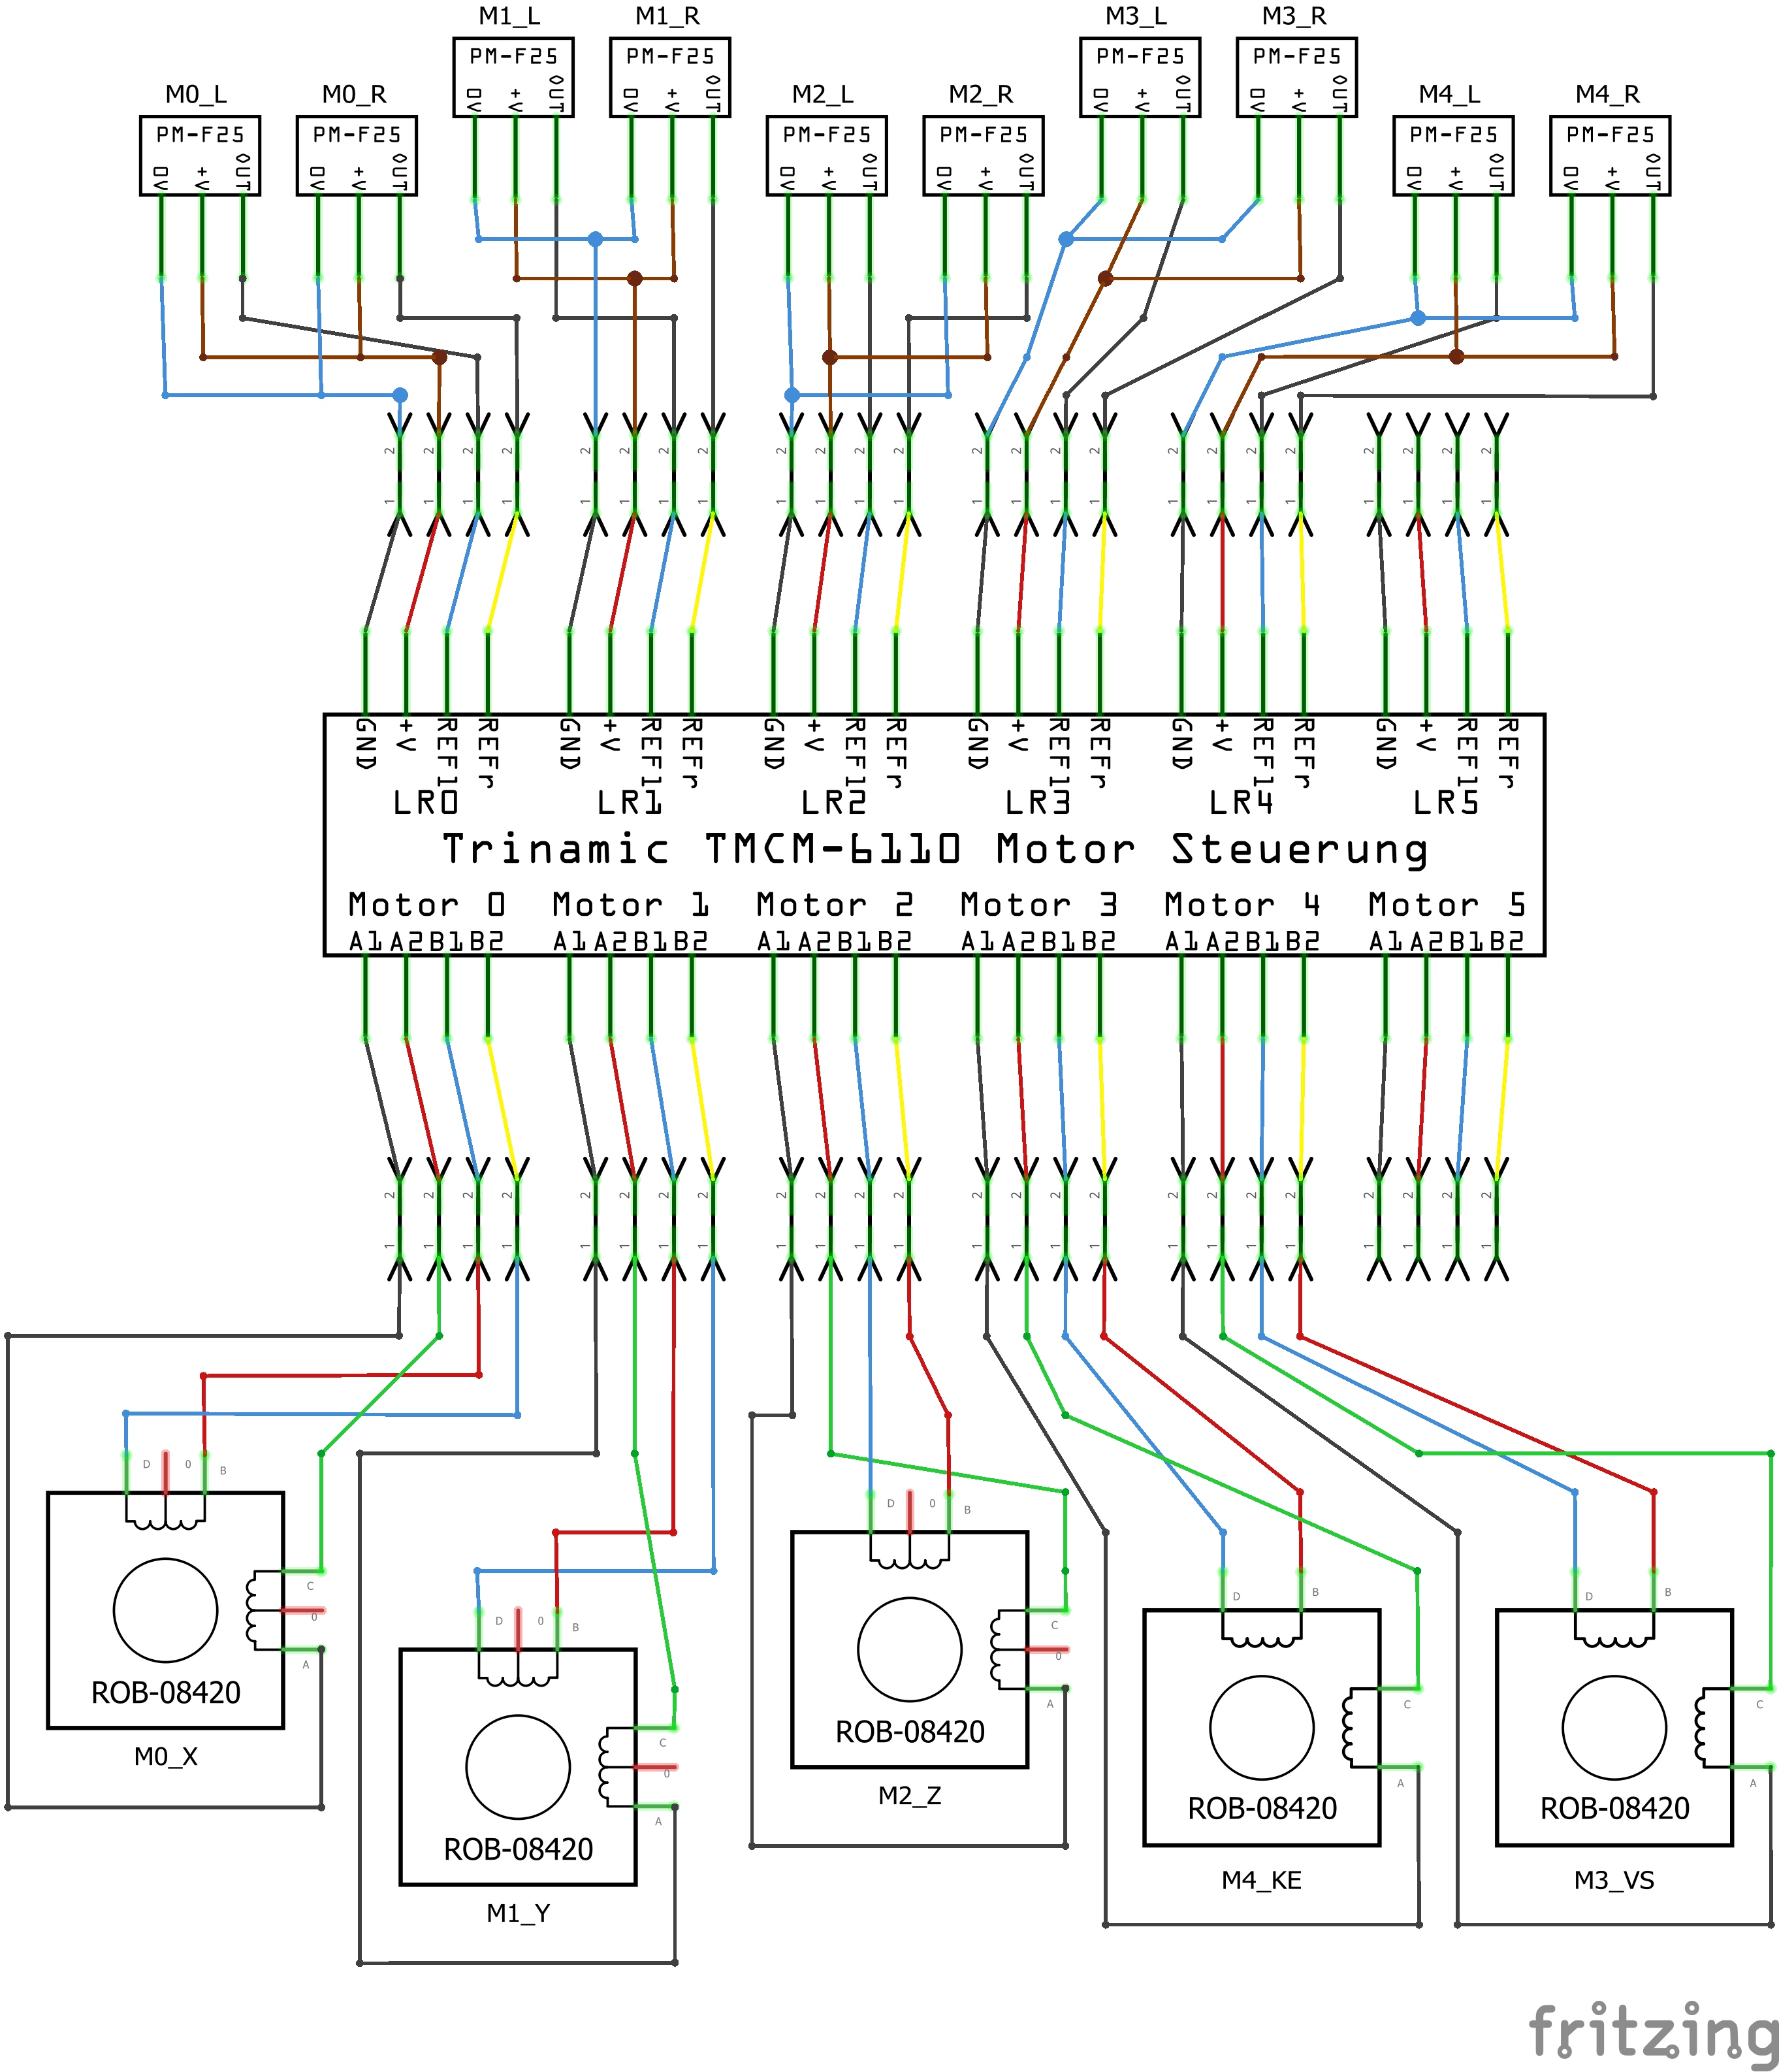
\includegraphics[width=\linewidth]{Anhang/TMCM_Motor_schem.png}
    \caption{Schematische Zeichnung der TMCM-6110 Motor Controller}
    \label{fig:tmcm_m}
\end{figure}

\subsection{TMCM-6110 IO Module}
\begin{figure}[H]
    \centering
    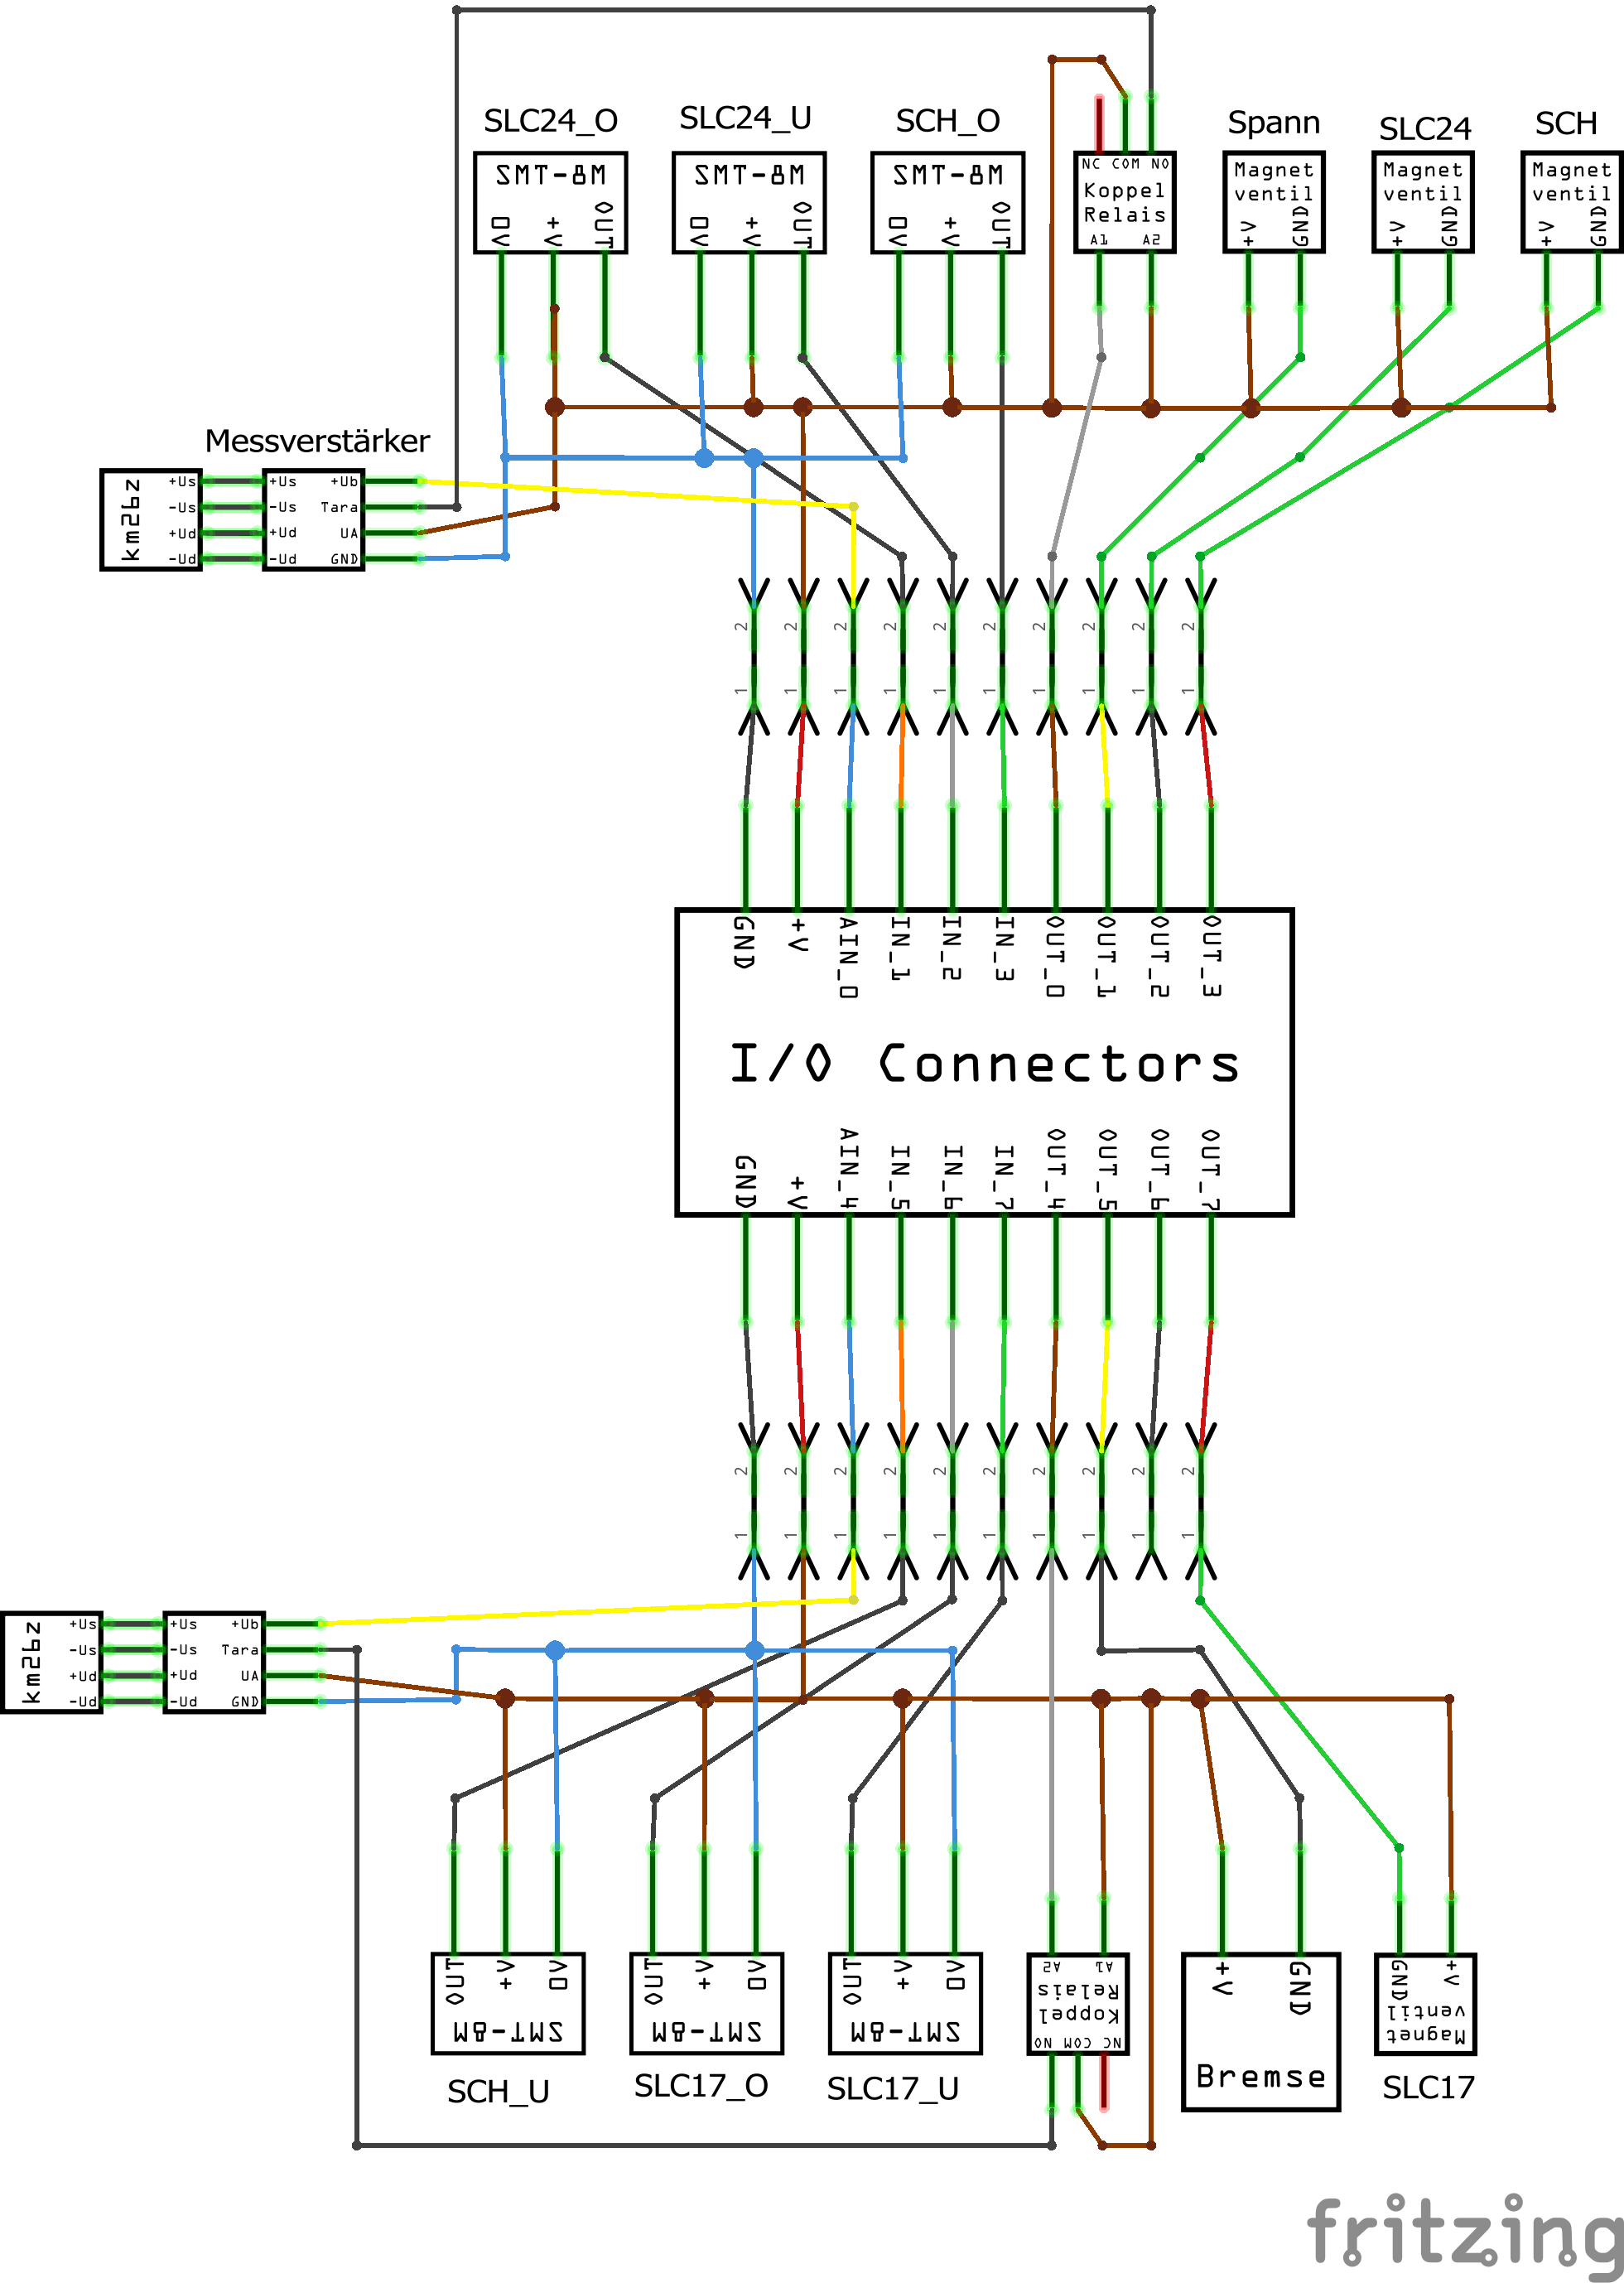
\includegraphics[width=\linewidth]{Anhang/TMCM_IO_schem.png}
    \caption{Schematische Zeichnung der TMCM-6110 IO Module}
    \label{fig:tmcm_io}
\end{figure}

\subsection{WAGO Module}
\begin{figure}[H]
    \centering
    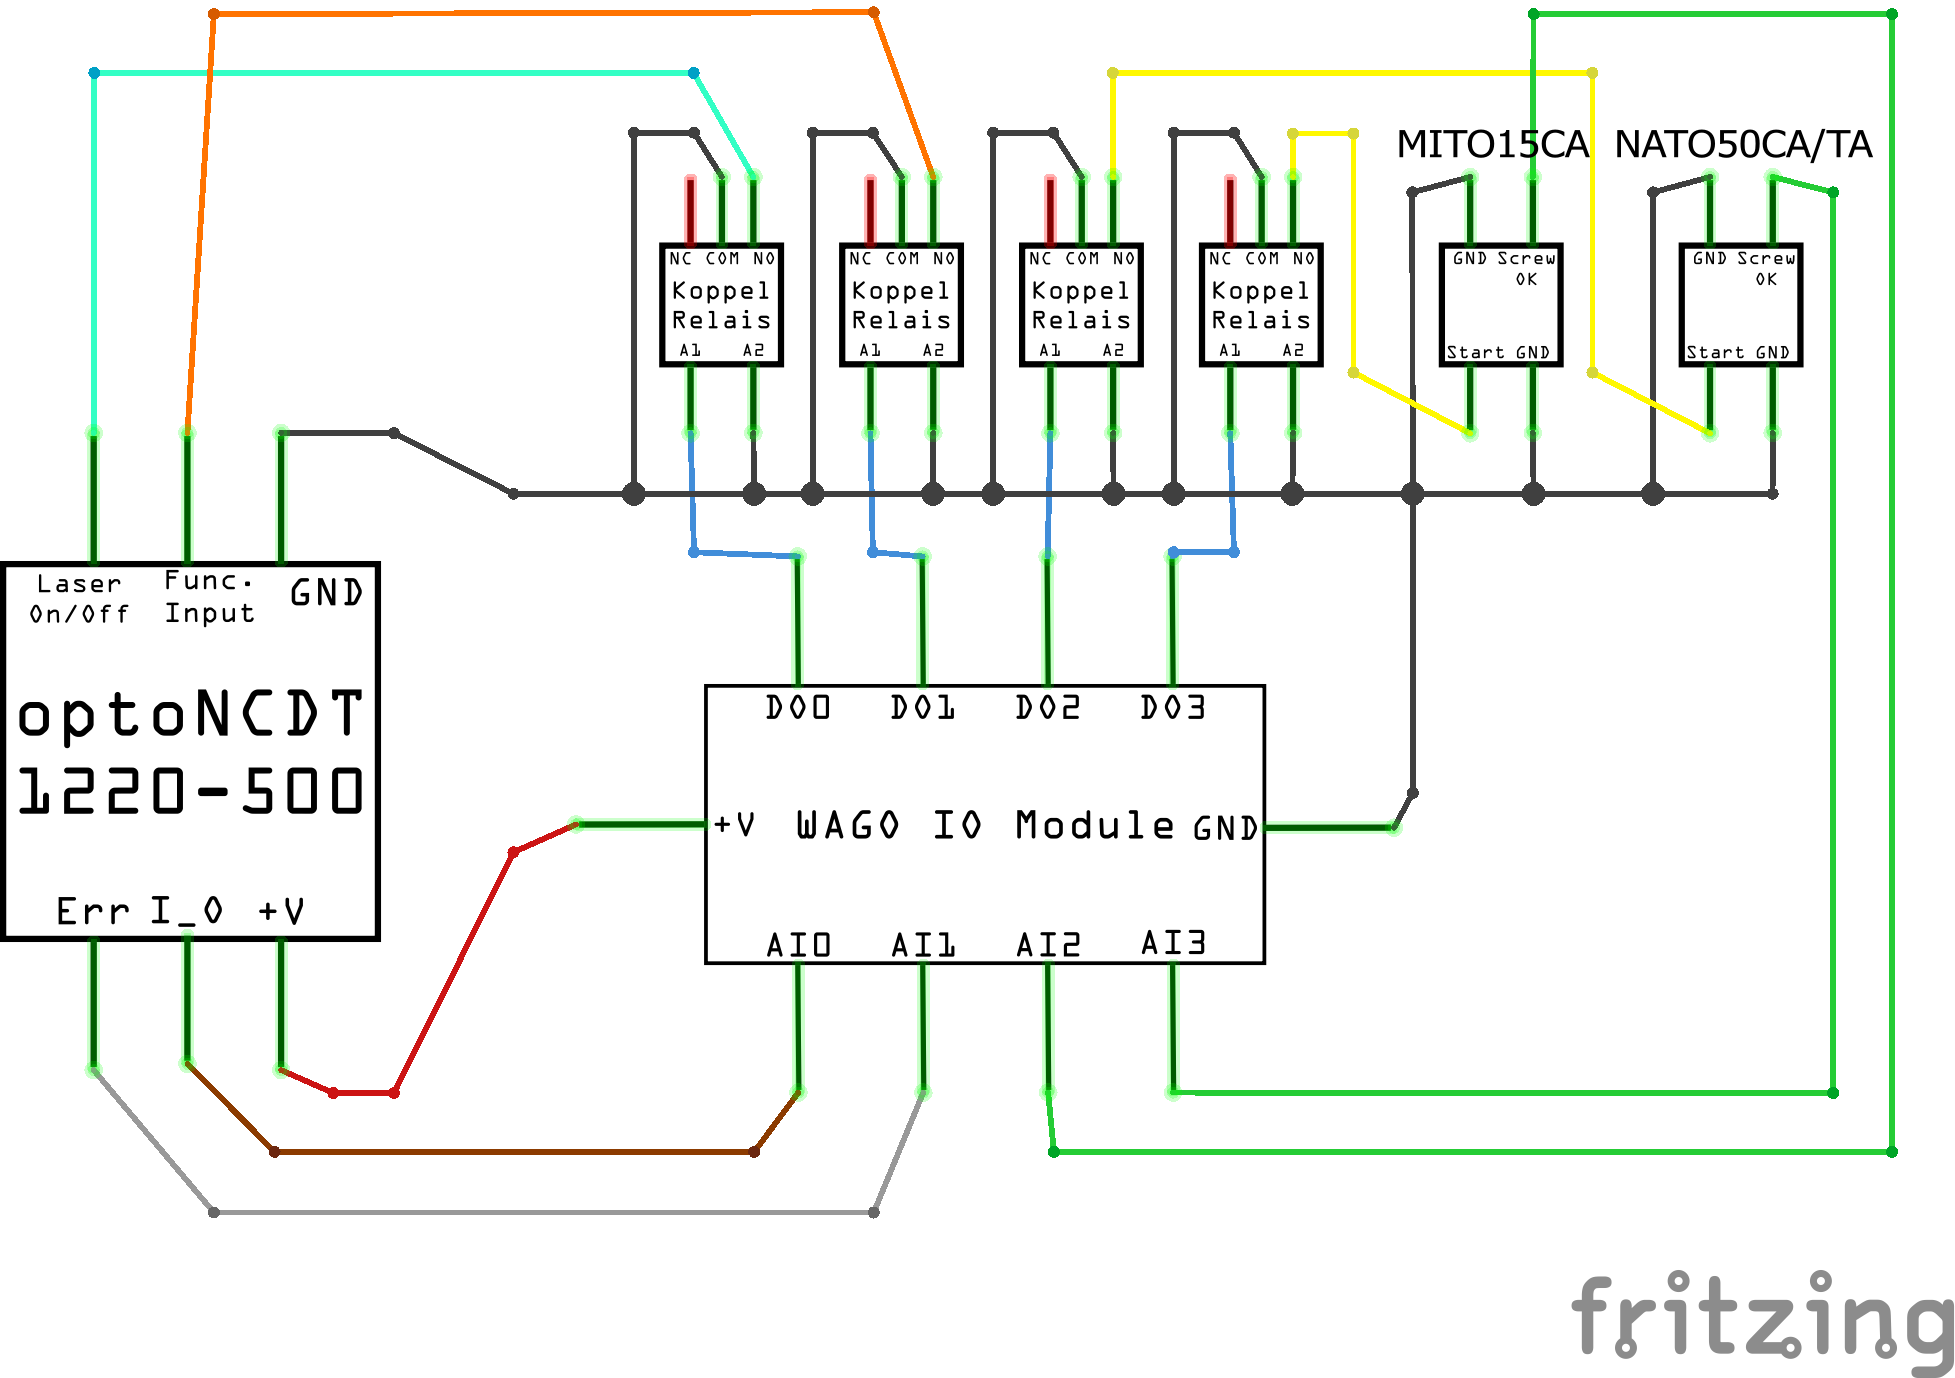
\includegraphics[width=\linewidth]{Anhang/WAGO_schem.png}
    \caption{Schematische Zeichnung der Wago Modul}
    \label{fig:wago}
\end{figure}

\clearpage

\section{Testskripte und Steuerungsprogramme}
\subsection{WAGO-Steuerung}
\subsubsection{WAGO GUI (Visualisierung)}
Das folgende Python-Programm (\texttt{gui.py}) implementiert eine einfache Benutzeroberfläche zur manuellen Ansteuerung digitaler Ausgänge sowie zur Anzeige der Eingangssignale (inkl. Laser-Skalierung). Das Programm wurde ausschließlich für Test- und Inbetriebnahmezwecke im Rahmen der Validierung verwendet.

\begin{lstlisting}[
    style=python-vsc,
    caption={Python GUI zur WAGO-I/O-Ansteuerung (gui.py)},
    label={lst:gui_py}]
# ----------------------------------------------------------
# Simple Tkinter-based graphical user interface for manual testing of a WAGO 750-362 I/O system via Modbus/TCP.
#
# The GUI allows:
# - Manual switching of digital outputs
# - Monitoring of digital and analog inputs
# - Scaling and visualization of a laser triangulation sensor signal
#
# The program was used exclusively for testing and validation purposes
# during the prototype phase of the system.
# ----------------------------------------------------------

import tkinter as tk
from tkinter import ttk, messagebox

# Import WAGO communication backend and configuration
from wago_io import (
    WagoConfig,
    WagoIO,
    DEFAULT_OUTPUT_NAMES,
    DEFAULT_INPUT_NAMES,)

class App(tk.Tk):
    """
    Main application class for the WAGO IO Monitor GUI.
    Handles user interaction, Modbus communication and cyclic polling.
    """

    def __init__(self):
        super().__init__()

        # Window configuration
        self.title("WAGO IO Monitor (Modbus/TCP)")
        self.geometry("600x440")

        # WAGO I/O interface instance
        self.io: WagoIO | None = None
        self.connected = False

        # Tkinter timer ID for cyclic polling
        self.after_id: str | None = None

        # Build the user interface
        self._build_ui()

    def _build_ui(self):
        """
        Creates all GUI elements (connection settings, IO display, buttons).
        """
        frm = ttk.Frame(self, padding=10)
        frm.pack(fill="both", expand=True)

        # --------------------------------------------------
        # Connection settings
        # --------------------------------------------------
        conn = ttk.LabelFrame(frm, text="Connection", padding=10)
        conn.pack(fill="x")

        ttk.Label(conn, text="IP:").grid(row=0, column=0, sticky="w")
        self.ip_var = tk.StringVar(value="192.168.1.31")
        ttk.Entry(conn, textvariable=self.ip_var, width=18).grid(
            row=0, column=1, sticky="w", padx=6)

        ttk.Label(conn, text="Port:").grid(row=0, column=2, sticky="w")
        self.port_var = tk.StringVar(value="502")
        ttk.Entry(conn, textvariable=self.port_var, width=6).grid(
            row=0, column=3, sticky="w", padx=6)

        self.btn_connect = ttk.Button(conn, text="Connect", command=self.on_connect)
        self.btn_connect.grid(row=0, column=4, padx=6)

        self.btn_disconnect = ttk.Button(
            conn, text="Disconnect", command=self.on_disconnect, state="disabled")
        self.btn_disconnect.grid(row=0, column=5)

        self.status_var = tk.StringVar(value="Disconnected")
        ttk.Label(conn, textvariable=self.status_var).grid(
            row=1, column=0, columnspan=6, sticky="w", pady=(8, 0))

        # --------------------------------------------------
        # Laser sensor scaling configuration
        # --------------------------------------------------
        laser = ttk.LabelFrame(frm, text="Laser scaling (4..20 mA -> mm)", padding=10)
        laser.pack(fill="x", pady=(10, 0))

        ttk.Label(laser, text="Start mm @4mA:").grid(row=0, column=0, sticky="w")
        self.laser_start_var = tk.StringVar(value="100.0")
        ttk.Entry(laser, textvariable=self.laser_start_var, width=10).grid(
            row=0, column=1, sticky="w", padx=6)

        ttk.Label(laser, text="End mm @20mA:").grid(row=0, column=2, sticky="w")
        self.laser_end_var = tk.StringVar(value="600.0")
        ttk.Entry(laser, textvariable=self.laser_end_var, width=10).grid(
            row=0, column=3, sticky="w", padx=6)

        ttk.Label(laser, text="AI FS counts:").grid(row=0, column=4, sticky="w")
        self.fs_var = tk.StringVar(value="32767")
        ttk.Entry(laser, textvariable=self.fs_var, width=8).grid(
            row=0, column=5, sticky="w", padx=6)

        # --------------------------------------------------
        # IO panels
        # --------------------------------------------------
        pan = ttk.Frame(frm)
        pan.pack(fill="both", expand=True, pady=(10, 0))

        # Digital Outputs
        out_box = ttk.LabelFrame(pan, text="Outputs (coils)", padding=10)
        out_box.pack(side="left", fill="both", expand=True, padx=(0, 5))

        self.out_vars: list[tk.IntVar] = []
        for i, name in enumerate(DEFAULT_OUTPUT_NAMES):
            v = tk.IntVar(value=0)
            self.out_vars.append(v)

            row = ttk.Frame(out_box)
            row.pack(fill="x", pady=2)

            ttk.Label(
                row, text=f"DO{i}: {name}", wraplength=260
            ).pack(side="left", fill="x", expand=True)

            ttk.Checkbutton(
                row,
                variable=v,
                command=lambda idx=i: self.on_toggle_output(idx)
            ).pack(side="right")

        btn_row = ttk.Frame(out_box)
        btn_row.pack(fill="x", pady=(8, 0))
        ttk.Button(btn_row, text="All OFF", command=self.all_off).pack(side="left", padx=(0, 6))
        ttk.Button(btn_row, text="All ON", command=self.all_on).pack(side="left")

        # Analog Inputs
        in_box = ttk.LabelFrame(pan, text="Inputs (input registers)", padding=10)
        in_box.pack(side="left", fill="both", expand=True, padx=(5, 0))

        self.in_labels: list[ttk.Label] = []
        for i, name in enumerate(DEFAULT_INPUT_NAMES):
            lbl = ttk.Label(in_box, text=f"AI{i}: {name} = -")
            lbl.pack(anchor="w", pady=2)
            self.in_labels.append(lbl)

        self.laser_label = ttk.Label(
            in_box,
            text="Laser distance (mm) = -",
            font=("Segoe UI", 10, "bold"))
        self.laser_label.pack(anchor="w", pady=(10, 2))

    def _apply_cfg_from_ui(self) -> WagoConfig:
        """
        Reads configuration values from the GUI and returns a WagoConfig object.
        """
        return WagoConfig(
            host=self.ip_var.get().strip(),
            port=int(self.port_var.get().strip()),
            laser_start_mm=float(self.laser_start_var.get().strip()),
            laser_end_mm=float(self.laser_end_var.get().strip()),
            ai_fullscale_counts=int(self.fs_var.get().strip()),)

    def on_connect(self):
        """
        Establishes the Modbus/TCP connection to the WAGO controller.
        """
        if self.connected:
            return

        try:
            cfg = self._apply_cfg_from_ui()
            self.io = WagoIO(cfg)
            ok = self.io.connect()
            if not ok:
                raise RuntimeError("Modbus connect failed.")
        except Exception as e:
            messagebox.showerror("Connect error", str(e))
            self.io = None
            return

        self.connected = True
        self.status_var.set(f"Connected to {self.io.cfg.host}:{self.io.cfg.port}")
        self.btn_connect.config(state="disabled")
        self.btn_disconnect.config(state="normal")

        # Start cyclic polling
        self._poll()

    def on_disconnect(self):
        """
        Disconnects from the WAGO controller and stops polling.
        """
        self._stop_poll()
        if self.io:
            try:
                self.io.close()
            except Exception:
                pass
        self.io = None
        self.connected = False
        self.status_var.set("Disconnected")
        self.btn_connect.config(state="normal")
        self.btn_disconnect.config(state="disabled")

    def _stop_poll(self):
        """
        Stops the cyclic polling loop.
        """
        if self.after_id is not None:
            try:
                self.after_cancel(self.after_id)
            except Exception:
                pass
            self.after_id = None

    def _poll(self):
        """
        Periodically reads inputs and outputs from the WAGO controller and updates the GUI.
        """
        if not self.connected or not self.io:
            return

        try:
            # Update configuration dynamically (laser scaling)
            try:
                new_cfg = self._apply_cfg_from_ui()
                self.io.cfg.laser_start_mm = new_cfg.laser_start_mm
                self.io.cfg.laser_end_mm = new_cfg.laser_end_mm
                self.io.cfg.ai_fullscale_counts = new_cfg.ai_fullscale_counts
            except Exception:
                pass

            # Read digital outputs
            outs = self.io.read_outputs()
            for i, val in enumerate(outs):
                if self.out_vars[i].get() != val:
                    self.out_vars[i].set(val)

            # Read analog inputs
            ins = self.io.read_inputs()
            for i in range(4):
                raw = ins.get(f"AI{i}_raw", float("nan"))
                mA = ins.get(f"AI{i}_mA", float("nan"))
                self.in_labels[i].config(
                    text=f"AI{i}: {DEFAULT_INPUT_NAMES[i]} = raw {raw:.0f} | {mA:.3f} mA")

            # Display scaled laser distance
            self.laser_label.config(
                text=f"Laser distance (mm) = {ins['Laser_mm']:.3f} mm   ({ins['Laser_mA']:.3f} mA)")

            self.status_var.set(f"Connected to {self.io.cfg.host}:{self.io.cfg.port}")

        except Exception as e:
            self.status_var.set(f"Error: {e}")

        # Poll at 5 Hz
        self.after_id = self.after(200, self._poll)

    def on_toggle_output(self, idx: int):
        """
        Writes a single digital output to the WAGO controller.
        """
        if not self.connected or not self.io:
            return
        try:
            val = int(self.out_vars[idx].get())
            self.io.set_output(idx, val)
        except Exception as e:
            messagebox.showerror("Write error", str(e))

    def all_off(self):
        """
        Switches all digital outputs OFF.
        """
        if not self.connected or not self.io:
            return
        try:
            for i in range(len(self.out_vars)):
                self.out_vars[i].set(0)
                self.io.set_output(i, 0)
        except Exception as e:
            messagebox.showerror("Write error", str(e))

    def all_on(self):
        """
        Switches all digital outputs ON.
        """
        if not self.connected or not self.io:
            return
        try:
            for i in range(len(self.out_vars)):
                self.out_vars[i].set(1)
                self.io.set_output(i, 1)
        except Exception as e:
            messagebox.showerror("Write error", str(e))


if __name__ == "__main__":
    # Start the GUI application
    App().mainloop()
\end{lstlisting}

\clearpage

\subsubsection{WAGO Backend (Prozesslogik)}
Das Backend-Programm bildet die grundlegende Prozesslogik der Anlage ab.
Hierzu zählen die Verknüpfung von Sensorsignalen, Sicherheitsabfragen sowie die logische Freigabe der Aktoren während der Tests.

\begin{lstlisting}[
    style=python-vsc,
    caption={WAGO Backend Code},
    label={lst:wago_backend}]
# ----------------------------------------------------------
# Helper module for WAGO 750-362 communication via Modbus/TCP.
#
# Hardware mapping used in the prototype:
# - Digital outputs (coils):     WAGO 750-531
# - Analog inputs (input regs):  2x WAGO 750-466  -> 4 channels total
# - Laser sensor: micro-epsilon optoNCDT 1220-500 (4..20 mA corresponds to 100..600 mm)
#
# Purpose:
# This module was used for manual testing and validation of I/O signals.
# It provides simple read/write functions and a conversion for the laser current signal.
# ----------------------------------------------------------

from dataclasses import dataclass
from typing import Dict, List, Optional

from pymodbus.client import ModbusTcpClient


@dataclass
class WagoConfig:
    """
    Configuration parameters for Modbus/TCP and the I/O mapping.
    Adjust start addresses/counts if the WAGO I/O order changes.
    """
    host: str = "192.168.1.31"
    port: int = 502

    # Digital outputs (WAGO 750-531)
    # Coils start address and number of outputs used in the project.
    do_coil_start: int = 0
    do_count: int = 4

    # Analog inputs (2x WAGO 750-466)
    # Input register start address and number of analog channels (4 total).
    ai_inputreg_start: int = 0
    ai_count: int = 4

    # Full-scale raw counts of the analog module (typical: 32767).
    ai_fullscale_counts: int = 32767

    # Laser sensor scaling
    # For optoNCDT 1220-500: 4 mA -> 100 mm and 20 mA -> 600 mm
    laser_start_mm: float = 100.0     # value at 4 mA
    laser_end_mm: float = 600.0       # value at 20 mA
    laser_ai_channel: int = 0         # which AI channel is used for the laser signal (AI0)


class WagoIO:
    """
    Lightweight Modbus/TCP interface for reading WAGO inputs and writing outputs.
    """

    def __init__(self, cfg: WagoConfig):
        self.cfg = cfg
        self.client: Optional[ModbusTcpClient] = None

    # ------------------------------------------------------
    # Connection handling
    # ------------------------------------------------------

    def connect(self) -> bool:
        """
        Create a Modbus/TCP client and connect to the WAGO controller.
        Returns True on successful connection.
        """
        self.client = ModbusTcpClient(
            host=self.cfg.host,
            port=self.cfg.port,
            timeout=2.0,)
        return bool(self.client.connect())

    def close(self) -> None:
        """
        Close the Modbus connection (if open).
        """
        if self.client:
            self.client.close()
        self.client = None

    def _ensure(self) -> ModbusTcpClient:
        """
        Internal helper: ensures that a connection exists.
        """
        if not self.client:
            raise RuntimeError("Not connected")
        return self.client

    # ------------------------------------------------------
    # Digital outputs (coils)
    # ------------------------------------------------------
    def read_outputs(self) -> List[int]:
        """
        Read the configured digital output states (coils).
        Returns a list with 0/1 values.
        """
        c = self._ensure()
        rr = c.read_coils(
            address=self.cfg.do_coil_start,
            count=self.cfg.do_count,)
        if rr.isError():
            raise RuntimeError(f"read_coils error: {rr}")

        # rr.bits contains booleans; convert to integer 0/1
        return [1 if b else 0 for b in rr.bits[:self.cfg.do_count]]

    def set_output(self, index: int, value: int) -> None:
        """
        Write one digital output (coil) by index.
        index: 0..do_count-1
        value: 0/1 (internally cast to bool)
        """
        if index < 0 or index >= self.cfg.do_count:
            raise ValueError("Output index out of range")

        c = self._ensure()
        rr = c.write_coil(
            address=self.cfg.do_coil_start + index,
            value=bool(value),)
        if rr.isError():
            raise RuntimeError(f"write_coil error: {rr}")

    # ------------------------------------------------------
    # Analog inputs (input registers)
    # ------------------------------------------------------
    def read_inputs_raw(self) -> List[int]:
        """
        Read analog input registers (raw counts).
        Returns a list of integer register values.
        """
        c = self._ensure()
        rr = c.read_input_registers(
            address=self.cfg.ai_inputreg_start,
            count=self.cfg.ai_count,)
        if rr.isError():
            raise RuntimeError(f"read_input_registers error: {rr}")

        return rr.registers[:self.cfg.ai_count]

    def raw_to_mA(self, raw: int) -> float:
        """
        Convert raw analog counts to an approximate current in mA.
        The conversion is scaled to 0..20 mA based on ai_fullscale_counts.
        """
        fs = float(self.cfg.ai_fullscale_counts)

        # Clamp raw signal to a valid range
        raw_f = max(0.0, min(float(raw), fs))

        # Map counts to 0..20 mA (sufficient for validation use)
        return (raw_f / fs) * 20.0

    def mA_to_distance_mm(self, mA: float) -> float:
        """
        Convert current (mA) to distance (mm) for the optoNCDT laser sensor.
        Uses linear scaling: 4..20 mA -> laser_start_mm..laser_end_mm.
        Values outside 4..20 mA are clamped.
        """
        x = (mA - 4.0) / 16.0
        x = max(0.0, min(1.0, x))
        return self.cfg.laser_start_mm + x * (
            self.cfg.laser_end_mm - self.cfg.laser_start_mm)

    def read_inputs(self) -> Dict[str, float]:
        """
        Read all analog inputs and return a dictionary with:
        - AIi_raw, AIi_mA for each channel
        - Laser_raw, Laser_mA, Laser_mm (derived from the configured laser channel)
        """
        raws = self.read_inputs_raw()
        currents = [self.raw_to_mA(r) for r in raws]

        # Extract laser channel values
        laser_raw = raws[self.cfg.laser_ai_channel]
        laser_mA = currents[self.cfg.laser_ai_channel]
        laser_mm = self.mA_to_distance_mm(laser_mA)

        # Build result dictionary (easy to use in GUI/logging)
        data: Dict[str, float] = {}
        for i, (r, mA) in enumerate(zip(raws, currents)):
            data[f"AI{i}_raw"] = float(r)
            data[f"AI{i}_mA"] = float(mA)

        data["Laser_raw"] = float(laser_raw)
        data["Laser_mA"] = float(laser_mA)
        data["Laser_mm"] = float(laser_mm)
        return data

# ----------------------------------------------------------
# Optional signal names (used by GUI and for consistent logging)
# ----------------------------------------------------------

DEFAULT_OUTPUT_NAMES = [
    "Laser Beam On/Off",
    "Laser Function Input",
    "Kolver NATO Start",
    "Kolver MITO Start",]

DEFAULT_INPUT_NAMES = [
    "Laser I_OUT",
    "Laser Error",
    "MITO SCREW_OK",
    "NATO SCREW_OK",]

\end{lstlisting}

\clearpage
\subsection{TMCM-6110 Testskript (TMCL-IDE)}
Das nachfolgende TMCL-Skript wurde im TMCL-IDE erstellt und diente zur Initialisierung sowie zum Test der einzelnen Linearachsen. Die Skripte wurden ausschließlich zu Validierungs- und Inbetriebnahmezwecken verwendet.

\begin{lstlisting}[
    style=tmcl-vsc,
    caption={TMCL-Testskript},
    label={lst:tmcl_test}]
// ---------------------------------------------------------
// TMCL Initialisierungsskript fuer Trinamic TMCM-6110
// Zweck:
// - Parametrierung der Achsen X, Y, Z, Keileinpressen, Vorspannen
// - Einfache Sicherheitsabschaltung ueber digitalen Eingang
// Einsatz: Inbetriebnahme und Validierung
// ---------------------------------------------------------

// ----------------------
// Allgemeine Einstellungen
// ----------------------

// Pull-Up Konfiguration digitale Eingaenge
// 0 = keine Pull-Ups
// 1 = Pull-Ups Achse 0-2
// 2 = Pull-Ups Achse 3-5
// 3 = Pull-Ups Achse 0-5
SGP 77, 0, 1        // Auto-Start aktivieren


// =========================================================
// Achse 1 (Kanal 0) - X-Achse
// =========================================================
SAP   4, 0, 2000    // maximale Positioniergeschwindigkeit
SAP   5, 0, 1000    // maximale Beschleunigung
SAP   6, 0, 200     // maximaler Motorstrom
SAP   7, 0, 30      // Haltestrom
SAP  12, 0, 0       // rechter Endschalter deaktiviert
SAP  13, 0, 0       // linker Endschalter deaktiviert
SAP 138, 0, 0       // Positioniermodus
SAP 140, 0, 5       // Mikroschrittauflosung
SAP 153, 0, 5       // Ramp Divider
SAP 154, 0, 5       // Pulse Divider
SAP 194, 0, 1000    // Referenzfahrgeschwindigkeit


// =========================================================
// Achse 2 (Kanal 1) - Y-Achse
// =========================================================
SAP   4, 1, 2000
SAP   5, 1, 1000
SAP   6, 1, 150
SAP   7, 1, 50
SAP  12, 1, 0
SAP  13, 1, 0
SAP 138, 1, 2       // Geschwindigkeitsmodus
SAP 150, 1, 1       // Endschalter Power-Down aktiv
SAP 140, 1, 4
SAP 153, 1, 5
SAP 154, 1, 5
SAP 194, 1, 2000


// =========================================================
// Achse 3 (Kanal 2) - Z-Achse
// =========================================================
SAP   4, 2, 2000
SAP   5, 2, 1000
SAP   6, 2, 150
SAP   7, 2, 30
SAP  12, 2, 0
SAP  13, 2, 0
SAP 138, 2, 0
SAP 140, 2, 4
SAP 153, 2, 5
SAP 154, 2, 5
SAP 194, 2, 2000


// =========================================================
// Achse 4 (Kanal 3) - Keileinpressen
// =========================================================
SAP   4, 3, 2000
SAP   5, 3, 1500
SAP   6, 3, 156
SAP   7, 3, 30
SAP  12, 3, 0
SAP  13, 3, 0
SAP 138, 3, 2
SAP 140, 3, 5
SAP 153, 3, 6
SAP 154, 3, 4
SAP 194, 3, 1200


// =========================================================
// Achse 5 (Kanal 4) - Vorspannen
// =========================================================
SAP   4, 4, 2000
SAP   5, 4, 200
SAP   6, 4, 160
SAP   7, 4, 30
SAP  12, 4, 0
SAP  13, 4, 0
SAP 138, 4, 0
SAP 140, 4, 6
SAP 153, 4, 5
SAP 154, 4, 5
SAP 194, 4, 1500


// =========================================================
// Sicherheitsueberwachung
// =========================================================

LOOP:
    GIO 8, 1            // digitalen Eingang lesen
    COMP 200            // mit Schwellwert vergleichen
    JC LT, MOTORSTOP    // wenn kleiner 200 -> Motorstop
    JA LOOP             // sonst weiter pruefen


// =========================================================
// Not-Stopp Routine
// =========================================================

MOTORSTOP:
    MST 0
    MST 1
    MST 2
    MST 3
    MST 4
    MST 5
    JA LOOP

STOP
\end{lstlisting}
\clearpage
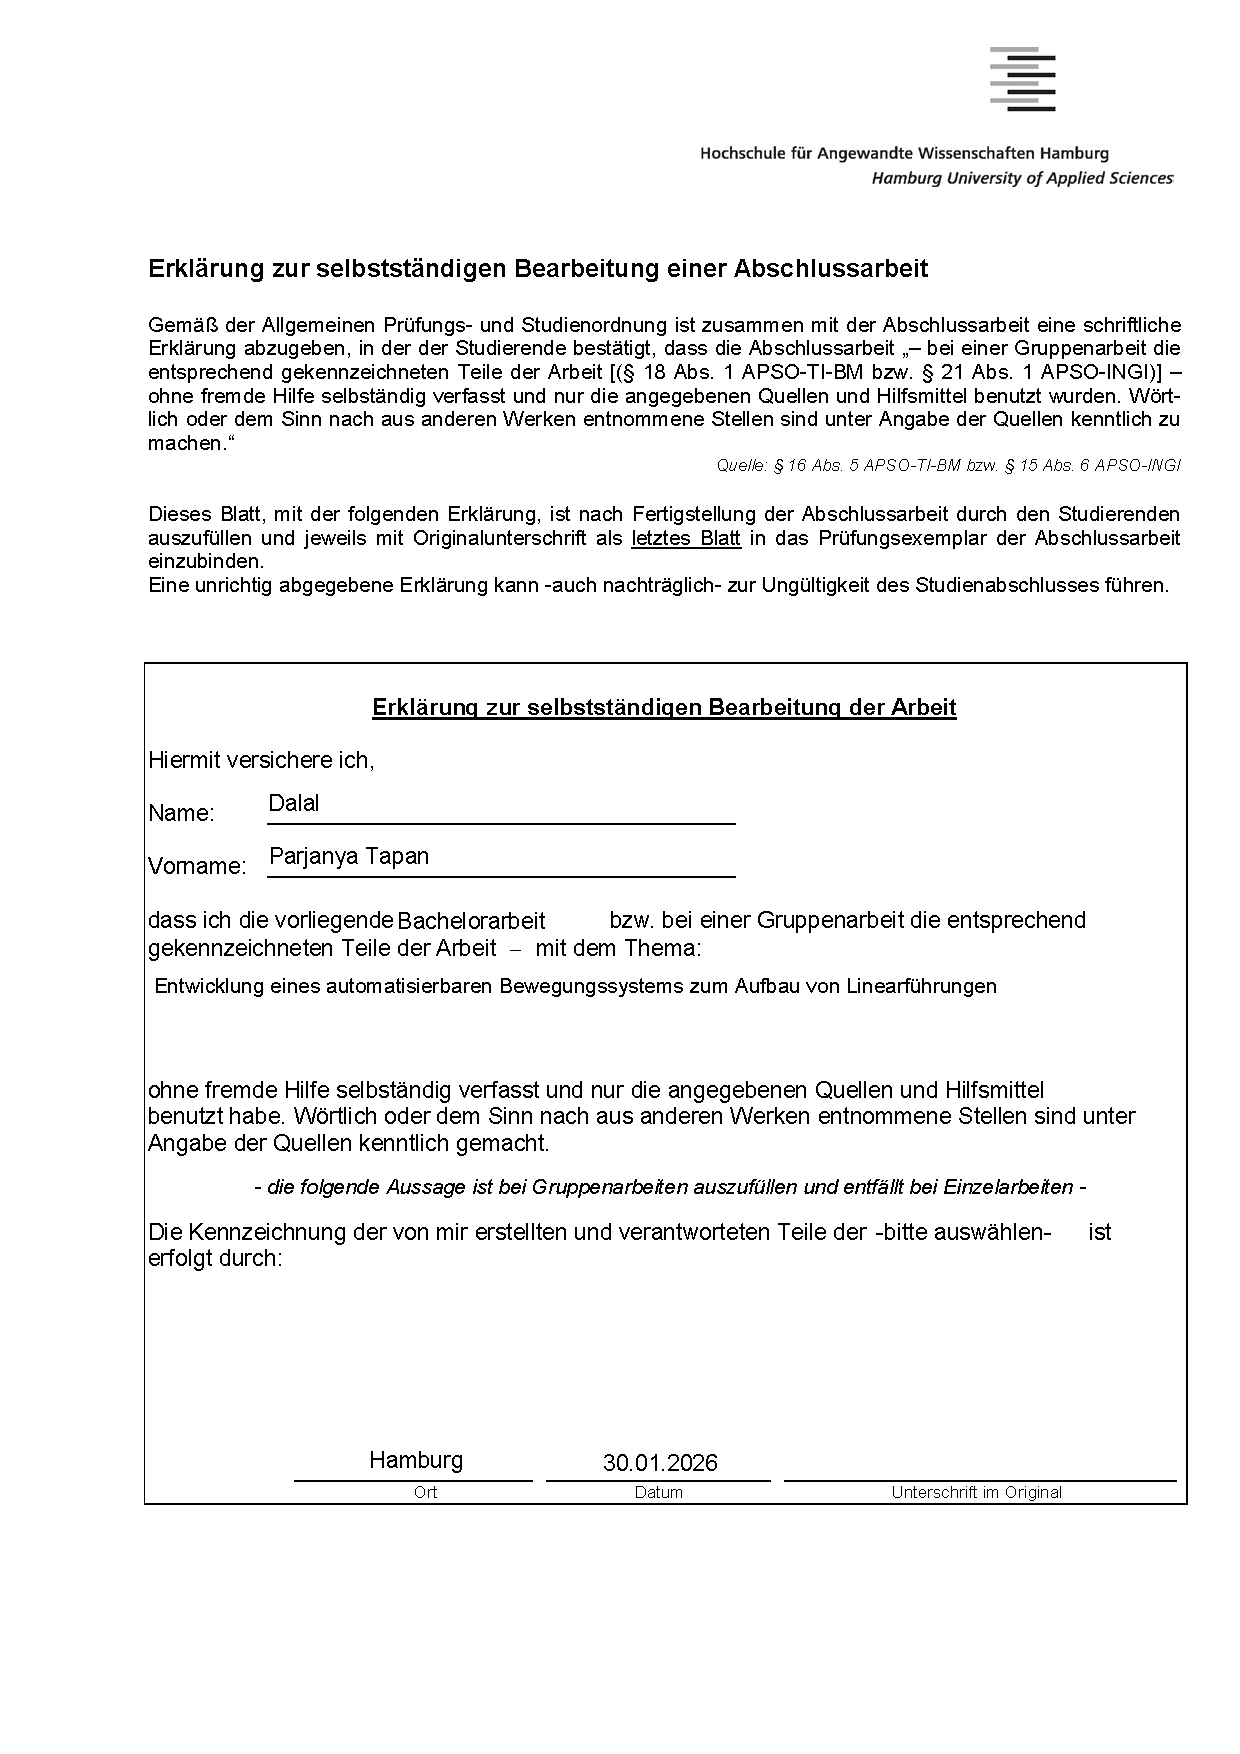
\includepdf{misc/Background/HAW_Stil/Selbststaendigkeitserklaerung.pdf}

\end{document}

